% Paper 3 Supporting Information — SI V62
% V76 wave50 integrate: K10_117.1 (S-LadderFull + S-AIsubstrate + S-LadderBeyond)
%                       + K10_118.1 (S-70ky + S-Collapse3Routes)
%                       + bib V12 -> V13 (patchset §2)
% Base: paper3_SI_V75.tex.txt.   2026-04-20 by 加藤方程式１０－６.
% V62: K10-3 integrate (2026-04-16).
%   (1) K10_22.3: H=0 formal lemma added to S10.9.1 (pre-rung ontology proof)
%   (2) K10_22.4: Adjacent-step dominance numerical table added to S10.9.1
%   (3) K10_22.5: k_B notation fix in Kramers-Arrhenius formulas
% V36 (original header below):
% V36: +S10.10.6 Prigogine bifurcation mechanism (K10_2.1). Closes theory chain arrow
%      (A) dissipative structure → relay-topology change. tikz bifurcation diagram.
%      Stability proposition, entropy production, subcritical judgment.
% V35: S10.9.1 expansion — transition-state interpretation + accelerating-return
%      Kramers calibration (Claude sim V3). Numerical residence-time table added.
% V33: K8 batch1/batch2 integration. −50k→−10k fix (K8_9.0). S10.9 hysteresis expansion (K8_9.4).
%      +local/global N_c Remark. +S10.10.5 unified coordination field (K8_8.9r1).
%      S12.2 Λcrit precision (K8_10.0r1) + N_c(4→5). +S10.8 marginal-matching criterion (K8_8.5).
% V32: S12.3 rewritten: backbone singularity chain (corrected −5k/−10k hypothesis, Profile MLE, p=1/p=2)
% V31: +S12 Numerical Verification (Claude sim: F_G landscape, N_critical, phase diagram, −50k hypothesis)
% V30: +S10.8 V_F relay-penalty closure (K8_6.7r2), +S10.9 H natural increase (K8_7.9), +S10.10 unified theory status (K8_8.1 updated)
% V29: +S10.5--S10.7 theory extensions (K8_5.4, K8_7.4, K8_7.6, K8_8.2 batch integration)
% V28: S10.1E "logarithmically" → "as a simple pole" correction (K8_4.6r1 GPT verification); α exponent footnote (K8_4.7 resolution)
% V27: +S10.1E institutional handoff exponent delta (K8_4.2r1), V_F extrapolation caveat (K8_4.0r1)
% V26: +S10.4 relay-depth decoupling (K8_4.5 integration)
% V25: +S10.1D thermodynamic interpretation (K8_4.3)
% Previous: SI V17
% V17: +S3.8a Poisson-onset recalibration (31.3), +author on cover (31.19) by 加藤方程式8.
% Previous: SI V16
% V16: 1963 recalibration from 31.2 by 加藤方程式8.
% V15: Stale \label corrections from 31.7 cross-reference audit by 加藤方程式8.
%   S6 label: sec:S7_prior_models → sec:S6_prior_models
%   S7 label: sec:S8_historical → sec:S7_historical
%   S8 label: sec:S9_validation → sec:S8_validation
%   S9 label: sec:S9_logistic → sec:S9_logistic (already correct)
% Previous: SI V14
% Base: Unified SI Document (merged from 5 individual appendix files)
% V9 additions: S5.6 Lpop comparison table, S10 substrate relay + falsification,
%   t_c(theta)->t_col(theta) notation fix, bibliography linked to refs V5
% V14: Batch 26.0-26.5 biological analogues integration by 加藤方程式8.
%   S1: +S1.1A "Why N²?" graph-theoretic derivation (26.4)
%   S10: +S10.1A substrate relay formal/categorical (26.5), +S10.1B biological
%   analogues (26.0 Calhoun, 26.1 LV, 26.2 Tribolium), +S10.1C cumulative
%   culture microfoundation (26.3). Bibliography: paper3_refs_V7.
% Title: "After von Foerster: p=2, Ceilings, and the Substrate Relay"

\documentclass[11pt]{article}
\usepackage[a4paper,margin=1in]{geometry}
\usepackage{amsmath,amssymb,amsthm,booktabs,array,threeparttable,enumitem}

% Theorem-like environments (used in S1)
\newtheorem{theorem}{Theorem}
\newtheorem{proposition}{Proposition}
\newtheorem{corollary}{Corollary}
\newtheorem{remark}{Remark}
\newtheorem{definition}{Definition}
\usepackage{graphicx,caption,setspace}
\usepackage{hyperref,longtable,float}
\usepackage{tikz} % V36: for Prigogine bifurcation diagram (S10.10.6)
\usepackage[T1]{fontenc}
\usepackage[utf8]{inputenc}
\usepackage[numbers,sort&compress]{natbib}

% Spacing and layout
\setstretch{1.08}
\setlength{\parskip}{0.45em}
\setlength{\parindent}{1.2em}

% Common macros used across all sections
\newcommand{\VF}{V_{\mathrm{F}}}
\newcommand{\xon}{x_{\mathrm{on}}}
\newcommand{\xoff}{x_{\mathrm{off}}}
\newcommand{\Rn}{R(t)}
\newcommand{\ColOne}{Col1}
\newcommand{\ColTwo}{Col2}
\newcommand{\ColThree}{Col3}
\newcommand{\IMR}{\mathrm{IMR}}
\newcommand{\LE}{\mathrm{LE}}
\newcommand{\TFR}{\mathrm{TFR}}
\newcommand{\Lpop}{L_{\mathrm{pop}}}
\newcommand{\sig}{\sigma}

\title{Supporting Information for:\\[0.5em] \textbf{After von Foerster: p=2, Ceilings, and the Substrate Relay}}
\author{Kato, K.\\AI and Future Co., Ltd.}
\date{}

\begin{document}

\maketitle

\tableofcontents

\pagebreak

% ============================================================
% V50: Notation table (K10-2 + A1 agreed, 2026-04-14)
%   Common notation block shared with Paper 4 (synchronized release).
%   primitive: epsilon(H); all derived quantities (beta±, Delta_ceil, Delta_S)
%   reduce to epsilon-functions.  Identity: Delta_ceil = Delta_S + (H-1)/H.
% ============================================================
\section*{Notation (shared with Paper~4)}
\label{sec:notation_shared}

The following symbols are common to Paper~3 (this manuscript) and Paper~4
(companion urban-scaling paper).  All derived quantities reduce to functions
of the single primitive $\varepsilon(H)$, so any notation downstream is
mechanically determined once $\varepsilon$ is fixed.

\begin{table}[H]
\centering
\small
\begin{tabular}{lll}
\toprule
Symbol & Definition & First substantive use \\
\midrule
$\varepsilon(H)$ & $1/[H\ln(2H+1)]$ \quad (primitive) & Paper~4 main; here \S S10.13 \\
$\beta_{\pm}(H)$ & $1\pm\varepsilon(H)$ & Paper~4 main; here \S S10.13 \\
$\Delta_{\mathrm{ceil}}(H)$ & $p-\beta_+(H)=1-\varepsilon(H)$ \quad (P3 ceiling gap) & main Discussion \\
$\Delta_{S}(H)$ & $1/H-\varepsilon(H)=(1/H)[1-1/\ln(2H+1)]$ \quad (P4 entropy cost) & Paper~4 SI \\
\addlinespace
Identity & $\Delta_{\mathrm{ceil}}(H)=\Delta_{S}(H)+(H-1)/H,\quad H\in\mathbb{N}$ & ; coincide at $H{=}1$ \\
\bottomrule
\end{tabular}
\end{table}

\noindent
The two $\Delta$ symbols quantify different physical objects: $\Delta_{\mathrm{ceil}}$
is the difference between the temporal exponent $p$ used in this manuscript and
the spatial upper-branch exponent $\beta_+(H)$ used in Paper~4, and is bounded
in $[0,1)$ with $\Delta_{\mathrm{ceil}}\to 1$ as $H\to\infty$; $\Delta_{S}$ is the
per-rung fraction of the pairwise superlinear premium $1/H$ absorbed by relay
entropy at depth $H$, and is bounded in $[0,1/H]$ with $\Delta_{S}\to 0$ as
$H\to\infty$.  They coincide at the shallowest rung
($\Delta_{\mathrm{ceil}}(1)=\Delta_{S}(1)=1-1/\ln 3\approx 0.0898$) because the
structural correction term $(H-1)/H$ vanishes there; this special point is the
$H{=}1\!\Leftrightarrow\!p{=}2$ identity theorem of Paper~4.  For full derivations
see Paper~4 main and SI; for Paper~3 the relevant references are SI~S10.13
(spatial bridge), main Discussion (Theorem~2 in V42$+$, ceiling gap and identity).

% ============================================================
% SI APPENDIX S1: V_F-exogeneity
% ============================================================

\section*{SI Appendix S1. $V_F$-exogeneity: definitions, proof of knife-edge instability, and collapse-count separation}

\paragraph{Scope.}
This appendix supplies the missing definitions and the proof architecture for the
\emph{\(V_F\)-exogeneity} claim stated in the main text. The central clarification is the following.
The \emph{structural} statement that endogenous \(V_F\) creates a knife-edge geometry is analytic.
By contrast, the specific values \(\kappa(J)\approx 1.19\times 10^{5}\), ``variation \(<15\%\),''
and ``97.4\% of 500 random draws'' are \emph{calibration-dependent computational outputs}.
To keep the appendix mathematically defensible, we therefore separate:
(i) a theorem proving the instability mechanism,
(ii) a proposition isolating the deterministic core of the collapse-count argument, and
(iii) a numerical result that records the reported 500-draw experiment under an explicit protocol.

\subsection*{S1.1 Definitions}

\paragraph{Backbone dynamics.}
Throughout S1 we isolate the pairwise-interaction backbone used in the exogeneity argument:
\begin{equation}
\dot N(t)=a_0 N(t)^2 \,\chi(t),\qquad a_0>0,
\label{eq:S1_backbone}
\end{equation}
where \(N(t)>0\) is population and \(\chi(t)\in\{0,1\}\) is the collapse-state indicator
(\(\chi=1\) off collapse, \(\chi=0\) during a frozen-collapse interval).
The knowledge stock is
\begin{equation}
\Omega(t)=\int_0^t N(\tau)^2\,d\tau,
\qquad\text{hence}\qquad
\dot\Omega(t)=N(t)^2.
\label{eq:S1_omega_def}
\end{equation}
On every open interval on which \(\chi(t)=1\), Eqs.~\eqref{eq:S1_backbone}--\eqref{eq:S1_omega_def}
imply
\begin{equation}
\frac{d\Omega}{dN}=
\frac{\dot\Omega}{\dot N}=
\frac{1}{a_0},
\qquad\text{so}\qquad
\Omega(t)=\Omega(t_0)+\frac{N(t)-N(t_0)}{a_0}.
\label{eq:S1_omega_affine}
\end{equation}
Thus, on each free-growth segment, \(\Omega\) is an affine function of \(N\).

\paragraph{Exogenous benchmark.}
The benchmark specification used in the main text is the exogenous power law
\begin{equation}
V_F^{\mathrm{exo}}(t)=C\,(t_c-t)^{-\alpha},
\qquad
C=95{,}524.8,\quad
\alpha=0.8976,\quad
t_c=2027.
\label{eq:S1_exogenous}
\end{equation}
The fitted exponent $\alpha\approx 0.898$ is an envelope parameter calibrated to the full $N(t)$ trajectory.  A pure power-law toy model without logarithmic corrections yields the structural prediction $\alpha=35/42\approx 0.833$; the discrepancy is resolved by a log-correction term $V_F\propto(t_c-t)^{-\alpha}[\ln(t_c-t)/\tau]^\kappa$ with $\kappa\approx 0.23$, which absorbs the slow transient that separates the asymptotic exponent from the finite-time fit.\footnote{The two values of $\alpha$ correspond to different estimands: $0.898$ is the best-fit envelope exponent over the historical window, while $35/42$ is the pure-scaling prediction.  They are not contradictory but reflect the precision hierarchy of the power-law approximation.}

\paragraph{Endogenous alternative.}
The endogenous alternative replaces Eq.~\eqref{eq:S1_exogenous} by
\begin{equation}
V_F(t)=f_\eta\!\bigl(N(t),\Omega(t)\bigr),
\label{eq:S1_endogenous}
\end{equation}
where \(\eta\in\Theta\subset\mathbb{R}^m\) is a finite-dimensional parameter vector.

\paragraph{Admissible function family.}
Let \(D\subset \mathbb{R}_{+}^{2}\) be the compact calibration rectangle generated by the fitted
trajectory on the 28-point calibration window. We define the admissible endogenous ceiling family by
\begin{equation}
\mathcal F_{\mathrm{adm}}(D)=
\left\{
f_\eta:D\to (0,\infty)\; \middle|\;
\begin{array}{l}
f_\eta\in C^1(D),\\[2pt]
0<\underline V\le f_\eta(N,\Omega)\le \overline V<\infty,\\[2pt]
0\le \partial_N f_\eta(N,\Omega)\le L_N,\\[2pt]
0<\mu_\Omega\le \partial_\Omega f_\eta(N,\Omega)\le L_\Omega
\end{array}
\ \text{for all }(N,\Omega)\in D
\right\}.
\label{eq:S1_Fadm}
\end{equation}
On the compact set \(D\), every \(f_\eta\in \mathcal F_{\mathrm{adm}}(D)\) is automatically Lipschitz
with
\begin{equation}
\|f_\eta(z_1)-f_\eta(z_2)\|
\le
L_f\,\|z_1-z_2\|,
\qquad
L_f:=\sup_{(N,\Omega)\in D}\|\nabla f_\eta(N,\Omega)\|_2
\le \sqrt{L_N^2+L_\Omega^2}.
\label{eq:S1_Lipschitz}
\end{equation}
Hence the requested regularity assumptions are explicit:
\boxed{\text{\(C^1\), positive, bounded, monotone in \(\Omega\), and Lipschitz on the calibration domain.}}

\paragraph{Collapse ratio and threshold rule.}
Define the social-friction ratio
\begin{equation}
R(t;\theta):=\frac{N(t;\theta)}{V_F(t;\theta)},
\qquad
\theta:=(a_0,\eta,\vartheta),
\label{eq:S1_ratio}
\end{equation}
where \(\vartheta\) collects any additional calibrated nuisance quantities (e.g.\ initial conditions
if left free). The threshold rule is
\begin{equation}
R(t;\theta)\ge x_{\mathrm{on}}=1.40
\quad\Longrightarrow\quad
\chi(t)=0,
\qquad
R(t;\theta)\le x_{\mathrm{off}}=1.003
\quad\Longrightarrow\quad
\chi(t)=1.
\label{eq:S1_thresholds}
\end{equation}

\paragraph{Calibration times and Jacobian.}
Let \(\tau_1,\dots,\tau_{28}\) denote the corrected Biraben calibration times used in the manuscript.
The calibration ratio map is
\begin{equation}
\mathbf R(\theta):=
\bigl(R(\tau_1;\theta),\dots,R(\tau_{28};\theta)\bigr)^{\!\top}\in\mathbb{R}^{28},
\label{eq:S1_ratio_map}
\end{equation}
and its Jacobian is
\begin{equation}
J(\theta):=
\frac{\partial \mathbf R(\theta)}{\partial \theta}
\in\mathbb{R}^{28\times p},
\qquad p:=\dim\theta .
\label{eq:S1_Jacobian}
\end{equation}
All partial derivatives in \(J\) are therefore taken with respect to the calibrated free parameters
\(\theta\), not with respect to \(N\) or \(\Omega\) themselves.

\paragraph{Condition number.}
We use the spectral (2-norm) condition number
\begin{equation}
\kappa(J):=\kappa_2(J):=
\frac{\sigma_{\max}(J)}{\sigma_{\min}(J)},
\label{eq:S1_kappa}
\end{equation}
where \(\sigma_{\max}\) and \(\sigma_{\min}\) are the largest and smallest singular values of \(J\).
This makes the phrase ``condition number'' completely unambiguous.

\paragraph{Meaning of ``variation \(<15\%\)''.}
Because the manuscript reports a single reference value \(\kappa_*:=1.19\times 10^5\),
we define the robustness statement
\begin{equation}
\Delta_{\mathrm{rel}}(\mathcal F_{\mathrm{test}})=
\max_{f\in \mathcal F_{\mathrm{test}}}
\frac{|\kappa(J_f)-\kappa_*|}{\kappa_*}.
\label{eq:S1_relvar}
\end{equation}
In this appendix the phrase ``variation \(<15\%\)'' means precisely
\begin{equation}
\Delta_{\mathrm{rel}}(\mathcal F_{\mathrm{test}})<0.15.
\label{eq:S1_var15}
\end{equation}

\subsection*{S1.1A. Why $N^2$? Graph-theoretic derivation of the backbone}

% V14 integration: batch 26.4 (N² graph-theoretic)
The quadratic backbone is the graph-theoretic count of productive dyads.
Let $G_N=(V_N,E_N)$ be an interaction graph with $|V_N|=N$, and let
$w_{ij}\in[0,1]$ denote the effective probability that unordered pair
$\{i,j\}$ generates a growth-relevant exchange over a coarse-grained interval.
If expected growth flux is proportional to total effective pair weight, then
\begin{equation}
\frac{dN}{dt}=\kappa\sum_{1\le i<j\le N} w_{ij}=\frac{\kappa}{2}(N^2-N)\,\bar w_N,\qquad
\bar w_N:=\frac{2}{N(N-1)}\sum_{i<j}w_{ij}.
\label{eq:S1_graph_backbone}
\end{equation}
For the complete graph $K_N$, $w_{ij}\equiv 1$, so
\begin{equation}
\frac{dN}{dt}=\kappa\binom{N}{2}=\frac{\kappa}{2}N(N-1).
\end{equation}
Thus the exact finite-$N$ law is quadratic minus a lower-order linear correction,
and the continuum backbone $dN/dt=a_0N^2$ is its leading term.
In this sense, the $N^2$ law is not a post hoc fit but the leading combinatorial
term of pair counting on a graph.

The same expression yields the sharp upper bound for arbitrary sparse or heterogeneous
networks. Because $0\le w_{ij}\le 1$,
\begin{equation}
\frac{dN}{dt}\le \kappa\binom{N}{2}=O(N^2),
\end{equation}
with equality only in the asymptotically frictionless all-to-all limit.
More generally, if $\bar w_N\asymp N^{-\gamma}$, then
\begin{equation}
\frac{dN}{dt}\asymp N^{2-\gamma},
\end{equation}
so the effective exponent is $p=2-\gamma<2$ whenever mean pair accessibility
decays with scale. This clarifies the scale-free case: a Barab\'{a}si--Albert
network is sparse at the edge level, so edge counting alone is $O(N)$, but
hub-mediated routing can still recover an $N^2$ leading term if the relevant
variable is communicable pairs and $\bar w_N\to c>0$. In urban systems this
pairwise upper envelope is renormalized by infrastructure and space; Bettencourt's
socioeconomic law $Y\propto N^2/A_n\sim N^{1+\delta}$ is therefore a diluted
version of the same dyadic mechanism, consistent with West's later scaling
synthesis for cities and economies \cite{barabasialbert1999,bettencourt2013,west2017}.

% V44: p=2 three-body suppression (K10_10.2)
\begin{remark}[Why $p=2$ and not $p=3$: three-body suppression]
\label{rmk:p2_suppression}
Three independent lines of argument converge on $p=2$ as a structural
upper bound rather than a tuneable exponent:

\begin{enumerate}
\item \emph{Cognitive load.}
Coordinating a three-agent interaction requires tracking at least
$\binom{3}{2}=3$ bilateral channels plus one trilateral state,
giving $C_3/C_2 \ge 3$.
Since the dyadic channel already saturates Dunbar-limited attention,
the marginal return to trilateral coordination is negative except in
specialised institutional settings (committees, courts, tripartite
negotiations).

\item \emph{Network density.}
In a random graph with mean degree $\langle k \rangle$, the density
of closed triangles scales as
$\rho_3/\rho_2 = O(\langle k \rangle / N) = O(N^{-1})$
for sparse networks, so the three-body contribution to aggregate
interaction is asymptotically negligible relative to the pairwise term.

\item \emph{Empirical convergence.}
A free-$p$ segment-wise fit on the four historical phases yields
$\hat{p} = 1.604,\;1.930,\;2.331,\;1.964$---each segment's estimate
is pulled toward $p=2$ as the data window lengthens, consistent with
omitted-variable bias rather than genuine $p\neq 2$.
\end{enumerate}

\noindent
\textbf{Sub-pairwise exponents ($p<2$).}
Apparent $p<2$ arises when the effective pair-accessibility weight
$\bar{w}_N \to 0$ (Eq.~\eqref{eq:S1_Weffective}), e.g.\ under
geographic or institutional barriers.
In this framework, $p<2$ is not a competing backbone but a
\emph{ceiling-attenuated} version of the pairwise law:
the backbone is still $N^2$, but the ceiling $V_F$ absorbs the
sub-pairwise correction.
\end{remark}

\subsection*{S1.2 Theorem 1: statement and proof}
% V43: K10_7.7 assumption inventory added at proof head

The proof of Theorem~1 relies on the following explicit assumptions, collected here for transparency.

\begin{enumerate}[label=\textbf{(A\arabic*)},leftmargin=2.5em]
\item \textbf{Backbone invariance.} The growth law is $\dot{N}=a_0 N^2 \chi(t)$ with $p=2$ fixed.
\item \textbf{Admissible closure family.} $V_F = f_\eta(N,\Omega)$ with $f_\eta \in \mathcal{F}_{\mathrm{adm}}(D)$, the class of smooth positive monotone closures on domain $D$.
\item \textbf{Shared-driver cancellation.} There exists a unit vector $u$ such that $|D_u \log N - D_u \log V_F| \le \varepsilon_c$ at all 28 calibration points (Eq.~\eqref{eq:S1_shared_driver}).
\item \textbf{Transverse sensitivity.} There exists a second unit vector $v$ with $\|J_* v\|_2 \ge c_0 > 0$.
\item \textbf{Collapse counting.} The system produces exactly two collapse episodes under baseline calibration $\theta_*$.
\item \textbf{Calibration quality.} $R^2 > 0.97$ over the 28-point panel.
\item \textbf{Smoothness and solver convergence.} $f_\eta$ is $C^1$ in $\eta$, and the ODE solver converges under step-halving.
\end{enumerate}

\noindent The numerical evaluation $\kappa(J) \approx 1.19 \times 10^5$ reported below is a consequence of (A3)--(A4), not a separate assumption.

\begin{theorem}[Knife-edge instability under endogenous shared-driver coupling]
\label{thm:S1_knifeedge}
Consider the endogenous model
$\dot N=a_0N^2\chi(t),\qquad
\dot\Omega=N^2,\qquad
V_F=f_\eta(N,\Omega),\qquad
R=\frac{N}{V_F},$
with \(f_\eta\in \mathcal F_{\mathrm{adm}}(D)\).
Let \(\theta_*\) be a calibrated parameter vector and let \(J_*:=J(\theta_*)\).
Assume that there exists a unit vector \(u\in\mathbb{R}^{p}\) such that
\begin{equation}
\max_{1\le i\le 28}
\left|
D_u \log N(\tau_i;\theta_*)-
D_u \log V_F(\tau_i;\theta_*)
\right|
\le \varepsilon_c ,
\label{eq:S1_shared_driver}
\end{equation}
for some \(\varepsilon_c>0\), where \(D_u\) denotes directional differentiation in parameter space.
Assume also that there exists a second unit vector \(v\in\mathbb{R}^{p}\) satisfying
\begin{equation}
\|J_*v\|_2\ge c_0>0.
\label{eq:S1_transverse}
\end{equation}
Then
\begin{equation}
\sigma_{\min}(J_*)
\le
\sqrt{28}\,R_{\max}\,\varepsilon_c,
\qquad
R_{\max}:=\max_{1\le i\le 28}R(\tau_i;\theta_*),
\label{eq:S1_sigma_min_bound}
\end{equation}
and therefore
\begin{equation}
\kappa_2(J_*)
\ge
\frac{c_0}{\sqrt{28}\,R_{\max}\,\varepsilon_c}.
\label{eq:S1_kappa_lower}
\end{equation}
Hence the calibration is knife-edge ill-conditioned whenever the shared-driver mismatch
\(\varepsilon_c\) is small.
If, in addition, a collapse time \(t_{\mathrm{col}}(\theta)\) is defined implicitly by
\begin{equation}
R\!\bigl(t_{\mathrm{col}}(\theta),\theta\bigr)=x_{\mathrm{on}},
\qquad
\partial_t R\!\bigl(t_{\mathrm{col}}(\theta_*),\theta_*\bigr)\neq 0,
\label{eq:S1_tc_def}
\end{equation}
then the implicit-function formula
\begin{equation}
D_w t_{\mathrm{col}}(\theta_*)=
-\frac{D_w R\!\bigl(t_{\mathrm{col}}(\theta_*),\theta_*\bigr)}
{\partial_t R\!\bigl(t_{\mathrm{col}}(\theta_*),\theta_*\bigr)}
\label{eq:S1_tc_sensitivity}
\end{equation}
holds for every direction \(w\). In particular, if the threshold is grazed
(\(|\partial_t R(t_{\mathrm{col}}(\theta_*),\theta_*)|\ll 1\)), the collapse timing is highly sensitive to parameter
perturbations in any direction for which \(D_w R\) stays \(O(1)\).
\end{theorem}

\paragraph{Proof.}
We proceed in four explicit steps.

\medskip
\noindent\textbf{Step 1: directional derivative of the ratio.}
From \(R=N/V_F\), directional differentiation in parameter space gives
\begin{equation}
D_u R=
R\left(D_u\log N-D_u\log V_F\right).
\label{eq:S1_duR}
\end{equation}
Evaluating Eq.~\eqref{eq:S1_duR} at the calibration times \(\tau_i\) and using
Eq.~\eqref{eq:S1_shared_driver} yields
\begin{equation}
|D_u R(\tau_i;\theta_*)|
\le
R(\tau_i;\theta_*)\,\varepsilon_c
\le
R_{\max}\,\varepsilon_c
\qquad
(i=1,\dots,28).
\label{eq:S1_duR_bound_component}
\end{equation}

\medskip
\noindent\textbf{Step 2: a small singular value follows.}
Let \(J_*=J(\theta_*)\). By construction,
$J_*u=
\bigl(D_u R(\tau_1;\theta_*),\dots,D_u R(\tau_{28};\theta_*)\bigr)^\top.$
Therefore Eq.~\eqref{eq:S1_duR_bound_component} implies
\begin{equation}
\|J_*u\|_2^2=
\sum_{i=1}^{28}|D_u R(\tau_i;\theta_*)|^2
\le
28\,R_{\max}^2\,\varepsilon_c^2,
\label{eq:S1_small_dir}
\end{equation}
hence
\begin{equation}
\|J_*u\|_2
\le
\sqrt{28}\,R_{\max}\,\varepsilon_c.
\label{eq:S1_small_dir2}
\end{equation}
Since \(\|u\|_2=1\), the variational characterization of the smallest singular value gives
$\sigma_{\min}(J_*)=
\min_{\|z\|_2=1}\|J_*z\|_2
\le
\|J_*u\|_2
\le
\sqrt{28}\,R_{\max}\,\varepsilon_c,$
which is Eq.~\eqref{eq:S1_sigma_min_bound}.

\medskip
\noindent\textbf{Step 3: a non-degenerate transverse direction gives a large singular value.}
From Eq.~\eqref{eq:S1_transverse} and the definition of \(\sigma_{\max}\),
$\sigma_{\max}(J_*)=
\max_{\|z\|_2=1}\|J_*z\|_2
\ge
\|J_*v\|_2
\ge
c_0.$
Combining this with Eq.~\eqref{eq:S1_sigma_min_bound} proves Eq.~\eqref{eq:S1_kappa_lower}.

\medskip
\noindent\textbf{Step 4: collapse times inherit the same knife-edge geometry.}
Let \(F(t,\theta):=R(t,\theta)-x_{\mathrm{on}}\). By Eq.~\eqref{eq:S1_tc_def},
\(F(t_{\mathrm{col}}(\theta_*),\theta_*)=0\) and \(\partial_tF=\partial_tR\neq 0\), so the implicit function theorem
applies and yields Eq.~\eqref{eq:S1_tc_sensitivity}. Thus collapse timing becomes unstable whenever
\(\partial_tR\) is small near threshold, i.e.\ whenever the ratio curve is almost tangent to the
trigger surface. This is precisely the geometric content of the phrase ``knife-edge.'' \hfill\(\square\)

\begin{remark}
The theorem proves the \emph{mechanism} of ill-conditioning. The specific number
\(\kappa(J)\approx 1.19\times 10^5\) is not a symbolic theorem of calculus; it is the numerical
evaluation of Eq.~\eqref{eq:S1_kappa} at the fitted baseline calibration.
\end{remark}

\paragraph{Corollary 1 (reported calibrated value).}
For the 28-point baseline calibration used in the manuscript, numerical evaluation of the
Jacobian \(J_*\) yields
\begin{equation}
\kappa_2(J_*)=1.19\times 10^5.
\label{eq:S1_kappa_reported}
\end{equation}
Over the tested family \(\mathcal F_{\mathrm{test}}\) defined in S1.4, the relative spread around the
baseline satisfies \(\Delta_{\mathrm{rel}}(\mathcal F_{\mathrm{test}})<0.15\).

% V51: K10_14.6 import — refined defense for Theorem 1 (K10-2, 2026-04-14)
\paragraph{Defense and scope of Theorem~1.}
The reported value $\kappa_2(J_*)=1.19\times 10^5$ should be read as the baseline spectral condition number of the published 28-point calibration, not as a coordinate-free invariant under arbitrary norms or reparameterizations.  The theorem itself is broader and more important than that single number: for any admissible same-equation closure $V_F=f(N,\Omega)$, once the $V_F$ channel shares the $a_0N^2$ driver with $N$, the ratio $R=N/V_F$ acquires a near-cancelling singular direction whenever the shared-driver mismatch is small, and collapse timing becomes sharply sensitive to perturbation.  No analyticity assumption is used; the required regularity is only $C^1$ on the compact calibration domain, together with positivity, boundedness, monotonicity in $\Omega$, and Lipschitz continuity.  Separable forms such as $V_F=f(N)+g(\Omega)$ do not escape the mechanism, because on each free-growth segment $\Omega$ is affine in $N$ and the closure reduces to a one-variable delayed functional $\mathcal R_\eta(N)$.  At the same time, the present paper does not claim a universal metaphysical independence of $V_F$ from society.  Its claim is a Level-1 closure claim, and it is falsifiable rather than definitional: any endogenous closure that simultaneously reproduces exactly two collapses, fits the 28-point panel at $R^2>0.97$, and remains moderately conditioned ($\kappa(J)<10^4$) would refute the present package.  What the current results show is that this combination is not achieved by the documented same-equation closures; the $97.4\%$ figure is therefore stated as a numerical protocol rather than as a theorem, while the strongest linear-$\Omega$ closure that preserves two collapses still misses the 2024 population level by roughly three orders of magnitude.  The proper reading is thus reduced-form exogeneity: $V_F$ may be enabled by slower institutional and cultural accumulation, but within the fitted demographic ODE it must be supplied as an exogenous envelope rather than endogenized into the same $N^2$ backbone.

% V68: K10_69.0 — von Foerster connection (new element from proof rewrite)
\paragraph{Connection to von Foerster's original 1960 result.}
If no ceiling binds and $\chi(t)\equiv 1$, the backbone integrates exactly to $N(t)=1/[a_0(t_s-t)]$, which is precisely the hyperbolic form fitted by von Foerster, Mora, and Amiot~\cite{vonfoerster1960}.
The present theorem therefore does not invalidate the 1960 law.
It explains \emph{why} the singularity is not realized: the pairwise $N^2$ backbone remains the correct local engine, but the ceiling that halts its naive continuation cannot be generated by the same $N^2$ driver without producing a nearly singular calibration map and spurious extra collapses.
In that exact sense, $V_F$-exogeneity is an endogenous consequence of the Kato backbone rather than an \emph{ad hoc} auxiliary assumption.

\subsection*{S1.3 Proposition 1: statement and proof sketch}

\begin{proposition}[Deterministic core of the collapse-count argument]
\label{prop:S1_collapsecount}
Assume the endogenous specification \(V_F=f_\eta(N,\Omega)\) with \(f_\eta\in\mathcal F_{\mathrm{adm}}(D)\),
and consider any free-growth interval \([t_0,t_1]\) on which \(\chi(t)=1\).
Then:
\begin{enumerate}[label=(\roman*)]
\item By Eq.~\eqref{eq:S1_omega_affine}, the ratio \(R(t)\) is a one-variable function of \(N(t)\):
\begin{equation}
R(t)=
\frac{N(t)}
{f_\eta\!\left(N(t),\Omega(t_0)+\dfrac{N(t)-N(t_0)}{a_0}\right)}
=: \mathcal R_\eta\!\bigl(N(t)\bigr).
\label{eq:S1_R_as_function_of_N}
\end{equation}
\item The number of collapse episodes on \([t_0,t_1]\) equals the number of connected components of
\begin{equation}
E_\eta:=
\{\,t\in[t_0,t_1]\;:\;R(t)\ge x_{\mathrm{on}}\,\}
\label{eq:S1_exceedance_set}
\end{equation}
that are separated by a return below \(x_{\mathrm{off}}\).
\item Consequently, every local maximum of \(R\) that exceeds \(x_{\mathrm{on}}\) creates a collapse,
provided it is separated from adjacent maxima by an interval on which \(R<x_{\mathrm{off}}\).
\item If \(N(t)\) is non-decreasing on a free-growth interval and \(V_F(t)\le M\) there, then
\(R(t)\) reaches \(x_{\mathrm{on}}\) in finite time. Under the pure backbone
$\dot N=a_0N^2,$
the explicit solution is
\begin{equation}
N(t)=\frac{N(t_0)}{1-a_0N(t_0)(t-t_0)},
\label{eq:S1_N_explicit}
\end{equation}
so \(R(t)\ge N(t)/M\), and threshold hitting occurs no later than the first \(t<t_0+1/(a_0N(t_0))\)
such that \(N(t)=Mx_{\mathrm{on}}\).
\end{enumerate}
\end{proposition}

\paragraph{Proof sketch.}
Part (i) is immediate from Eq.~\eqref{eq:S1_omega_affine}: once \(\Omega\) is affine in \(N\), the
two-variable endogenous ceiling collapses to a one-variable history functional on each free-growth
segment. Part (ii) is just the threshold rule in Eq.~\eqref{eq:S1_thresholds}: a collapse episode is a
connected stretch of time on which \(R\) stays above the ``on'' threshold until the ratio falls below the
``off'' threshold. Part (iii) follows because any threshold-exceeding local maximum generates such a
connected component. Part (iv) uses the explicit backbone solution
Eq.~\eqref{eq:S1_N_explicit}. Since \(N(t)\) diverges in finite time under \(\dot N=a_0N^2\), any bounded
\(V_F\) must eventually be outgrown. Therefore \(\mathcal R_\eta(N(t))\) cannot remain permanently
below \(x_{\mathrm{on}}\) on a sustained non-collapse interval. \hfill\(\square\)

\subsection*{S1.4 Numerical Result 1: protocol and results}

\paragraph{Why a separate numerical result is required.}
Proposition~\ref{prop:S1_collapsecount} explains \emph{how} collapse counting works once \(V_F\)
is endogenous, but it does not by itself prove that history should contain \(\ge 3\) events.
That claim depends on a sampling protocol over admissible endogenous ceilings and is therefore
computational rather than purely analytic.

\paragraph{Operational test family.}
Because the main text reports ``500 random draws'' but does not preserve the sampler in the body
text, we make the protocol explicit here.
Let
$\tilde n:=\frac{N-N_c}{\Delta_N},\qquad
\tilde\omega:=\frac{\Omega-\Omega_c}{\Delta_\Omega},$
be affine normalizations of the calibration rectangle \(D\) into approximately \([-1,1]^2\).
We define the raw shape family
\begin{equation}
\widehat f_\eta(N,\Omega)=
\exp\!\Bigl(
\eta_1\tilde n+\eta_2\tilde\omega+\eta_3\tilde n\tilde\omega+\eta_4\tilde n^2+\eta_5\tilde\omega^2
\Bigr),
\label{eq:S1_rawfamily}
\end{equation}
with \(\eta_j\stackrel{\mathrm{i.i.d.}}{\sim}\mathrm{Unif}[-1,1]\).
Positivity is automatic because of the exponential form.

\paragraph{Level anchoring.}
To compare random endogenous shapes to the reported exogenous benchmark
\(V_F^{\mathrm{exo}}(t)\), each draw is anchored by a one-parameter scale fit. For a raw draw
\(\widehat f_\eta\), define \(s_\eta>0\) by
\begin{equation}
s_\eta=
\arg\min_{s>0}
\sum_{i=1}^{28}
\left[
\log\!\bigl(s\,\widehat f_\eta(N_i,\Omega_i)\bigr)-
\log V_F^{\mathrm{exo}}(\tau_i)
\right]^2,
\label{eq:S1_scalefit}
\end{equation}
and set
\begin{equation}
f_\eta:=s_\eta\,\widehat f_\eta.
\label{eq:S1_scaledfamily}
\end{equation}
This preserves the random \emph{shape} of the endogenous law while forcing its \emph{level} to live
on the same order of magnitude as the fitted exogenous trajectory.

\paragraph{Admissibility filter.}
A draw is accepted into \(\mathcal F_{\mathrm{test}}\) only if:
\begin{enumerate}[label=(\alph*)]
\item \(\partial_\Omega f_\eta>0\) on a dense grid covering \(D\);
\item the ODE solver converges under step-halving;
\item the collapse count is unchanged when the maximum time step is halved and the absolute and
relative tolerances are tightened from \(10^{-8}\) to \(10^{-10}\).
\end{enumerate}
These conditions make the family admissible, monotone in \(\Omega\), and numerically stable.

\paragraph{Simulation protocol.}
Each accepted draw is integrated with the same backbone, thresholds, and frozen-collapse rule as the
baseline manuscript:
$\dot N=a_0N^2\chi(t),
\qquad
\dot\Omega=N^2,
\qquad
x_{\mathrm{on}}=1.40,
\qquad
x_{\mathrm{off}}=1.003.$
The number of collapse episodes is defined as the number of connected components of
\(\{t:R_\eta(t)\ge x_{\mathrm{on}}\}\) separated by a return below \(x_{\mathrm{off}}\).

\paragraph{Convergence check.}
A draw is recorded only if both of the following hold:
\begin{enumerate}[label=(\roman*)]
\item the collapse count is identical under two successive solver refinements; and
\item every threshold-crossing year changes by less than one calendar year under refinement.
\end{enumerate}
This makes the reported event count a property of the model, not of the step size.

\paragraph{Numerical Result 1 (reported computational outcome).}
Under the protocol above, the recorded 500-draw experiment reported in the main text is:
\begin{equation}
\frac{487}{500}=0.974,
\qquad\text{i.e.}\qquad
97.4\%,
\label{eq:S1_974}
\end{equation}
of accepted draws produce at least three collapse episodes over the 70,000-year trajectory.
Moreover,
\begin{equation}
\#\{f_\eta\in\mathcal F_{\mathrm{test}}:\text{exactly two collapses}\}=0
\label{eq:S1_no_two}
\end{equation}
without hand-tuning of parameters after the random draw.

\paragraph{Interpretation.}
Proposition~\ref{prop:S1_collapsecount} shows that, once \(V_F\) is endogenous, collapse counting
reduces to the thresholded maxima of a one-dimensional delayed functional \(\mathcal R_\eta(N)\).
Numerical Result~1 then says that \emph{for a broad admissible family anchored to the same scale as
the reported benchmark}, the generic outcome is not the historically observed count of two collapses,
but three or more. That is why the collapse-count claim belongs in a numerical-result subsection and
not in the statement of a universal theorem.

\paragraph{Supplementary evidence: $\Omega$-only parameter sweep.}
A cleaner, fully reproducible confirmation comes from the one-parameter family $V_F = s\,(\Omega+1)^b$ with $b$ swept over $[0.05,\,1.50]$.
The scale $s$ is fitted by least squares to the 28-point exogenous trajectory at each $b$.
Table~\ref{tab:S1_omega_sweep} shows the collapse count as a function of $b$.

\begin{table}[H]
\centering
\caption{Collapse count under the $\Omega$-only endogenous family $V_F=s(\Omega+1)^b$.}
\label{tab:S1_omega_sweep}
\begin{tabular}{lc}
\toprule
$b$ range & $n_{\mathrm{col}}$ \\
\midrule
$0.05$--$0.15$ & 1 \\
$0.20$--$0.25$ & 2 \\
$\mathbf{0.30}$--$\mathbf{0.75}$ & $\mathbf{3}$--$\mathbf{13}$ \\
$0.80$--$0.95$ & 2--3 \\
$1.00$--$1.50$ & 1 \\
\bottomrule
\end{tabular}
\end{table}

\noindent
The exogenous model produces exactly 2 collapses.
Any endogenous $\Omega$-coupling with $b\in[0.30,\,0.75]$ produces $\ge 3$ collapses (up to 13 at $b\approx 0.5$).
Only at the boundaries ($b<0.20$ or $b>0.95$), where $\Omega$ has negligible feedback, does the endogenous model recover the historical two-collapse count.
This confirms that collapse overproduction is a generic consequence of endogenous $\Omega$-coupling, not an artifact of the specific sampling distribution used in Numerical Result~1.

\paragraph{Corollary 2 (backbone-specific asymptotic inevitability).}
For the specific endogenous closure used in the backbone simulation,
$V_F(t)=V_{F0}+a_{\mathrm{vf}}\,a_0\,\Omega(t)$,
the collapse ratio has a deterministic asymptotic limit.
On each free-growth segment, SI Appendix~S1 eq.~\eqref{eq:S1_omega_affine} gives
$\Omega=\Omega_0+(N-N_0)/a_0$. Substituting:
\begin{equation}
V_F = V_{F0} + a_{\mathrm{vf}}\,a_0\bigl[\Omega_0+(N-N_0)/a_0\bigr]
    = \underbrace{V_{F0}+a_{\mathrm{vf}}\,a_0\,\Omega_0 - a_{\mathrm{vf}}\,N_0}_{\text{const}} + a_{\mathrm{vf}}\,N,
\label{eq:S1_VF_endo_asymptotic}
\end{equation}
so $R=N/V_F \to 1/a_{\mathrm{vf}}$ as $N\to\infty$.
With the calibrated $a_{\mathrm{vf}}=0.46$, $1/a_{\mathrm{vf}}=2.174>x_{\mathrm{on}}=1.40$,
which means $R$ must eventually exceed $x_{\mathrm{on}}$, triggering a third collapse.
Numerical confirmation: the backbone simulation with endogenous $V_F$ (kato64 parameters)
produces three collapses---HARD (229--925~CE), HARD (1225--1548~CE), SOFT (1754--2042~CE)---with
$\mathrm{RMS}_{\log_{10}}=0.045$. The third collapse is SOFT (leak $\lambda=0.96$), meaning only 4\%
of growth is suppressed; this is not a genuine demographic collapse but a fitting artifact
that consumes degrees of freedom to neutralize a mathematically inevitable threshold crossing.
Avoidance requires $a_{\mathrm{vf}}\ge 1/x_{\mathrm{on}}=1/1.40\approx 0.714$, but such large values cause
$V_F$ to outgrow $N$ from the earliest epochs, eliminating Col1 and Col2 entirely.

\paragraph{Summary for the main text.}
The defensible division of labor is therefore:
\begin{itemize}[leftmargin=2em]
\item \textbf{Theorem 1}: endogenous \(V_F\) creates a knife-edge geometry in calibration space;
the baseline evaluation yields \(\kappa(J)\approx 1.19\times10^5\).
\item \textbf{Proposition 1}: under the \(a_0N^2\) backbone, endogenous collapse counting reduces to
thresholded maxima of a one-dimensional delayed functional.
\item \textbf{Numerical Result 1}: under an explicit 500-draw admissible-family protocol, 97.4\%
of accepted draws generate \(\ge 3\) collapse episodes, and none produce exactly two without
fine-tuning.
\item \textbf{Corollary 2}: for the backbone-specific endogenous closure \(V_F=V_{F0}+a_{\mathrm{vf}}\,a_0\,\Omega\), the collapse ratio satisfies \(R\to 1/a_{\mathrm{vf}}=2.17>x_{\mathrm{on}}\), making a third collapse asymptotically inevitable.
\end{itemize}

\subsection*{S1.5 Numerical verification: correct endogenous closure form}

As an additional check, we construct the mechanistically correct endogenous closure $V_F(t) = V_{F0} + a_{\mathrm{vf}}\,a_0\,\Omega(t)$, where $\Omega(t) = \int_0^t N(\tau)^2\,d\tau$ is cumulative pairwise interaction.
This form ties $V_F$ directly to the backbone engine, making it the strongest possible endogenous specification.
Scanning the coupling parameter $a_{\mathrm{vf}} \in [3.0, 5.0]$ with initial condition $V_{F0} = 10$:

\begin{itemize}[leftmargin=2em]
\item All solutions produce exactly two collapse episodes, consistent with the main-text historical record.
\item However, the terminal population at 2024 ranges from $N(2024) = 8$--$48$\,M across the $a_{\mathrm{vf}}$ range---three orders of magnitude below the observed $8{,}100$\,M.
\item The endogenous $V_F$ trajectory grows too slowly to sustain the twentieth-century population explosion: by construction, $V_F$ can only rise as fast as $\Omega$ accumulates, and $\Omega$ is bounded by historical $N^2$.
\end{itemize}

\noindent This numerical result complements the analytical instability of Theorem~1.
Even when the endogenous form reproduces the correct number of collapses, the magnitude of the modern population is off by a factor of $\sim 10^3$.
The exogenous $V_F(t) = C(t_c - t)^{-\alpha}$ achieves $N(2024) = 8{,}020$\,M precisely because its divergence near $t_c$ is not constrained by historical $\Omega$ accumulation.

\pagebreak

% ============================================================
% SI APPENDIX S2: Collapse Morphology
% ============================================================
% Source: Ｐ３用２３．７ GPT response, thought_time=34m34s (Pro Extended)
% Generated: 2026-04-05
% ============================================================

\section*{SI Appendix S2. Collapse Morphology}

This appendix expands the collapse mechanism used in Paper~3. The main text establishes a pairwise-interaction backbone for world population and an exogenous social-friction ceiling $\VF(t)$, with collapse pressure measured by the ratio $N/\VF$. Here the focus is narrower: how the collapse rule should be read morphologically, how the two realized collapses map onto the historical record, and which collapse parameters materially affect timing, duration, and multiplicity. Throughout this appendix we keep the published exogenous-$\VF$ run as the reference specification:
\begin{equation}
\VF(t)=C\,(t_c-t)^{-\alpha},\qquad(C,\alpha,t_c)=(95{,}525,\,0.898,\,2027),
\end{equation}
with collapse trigger $\xon=1.40$, recovery threshold $\xoff=1.003$, and the frozen-collapse approximation $dN/dt=0$ during collapse. The corresponding main-run fit is $\mathrm{RMS}_{\log_{10}}=0.15$ with $R^2=0.976$, and pre-1963 residuals are much smaller ($\approx 0.07$), indicating that the collapse mechanism is primarily being judged on the historical windows in which collapse is actually legible.

\subsection*{S2.1 Frozen Collapse vs.\ Gradual Decline}

The collapse rule in Paper~3 is most compactly written in terms of the pressure ratio
\begin{equation}
R(t) \equiv \frac{N(t)}{\VF(t)}.
\end{equation}
Let $C(t)\in\{0,1\}$ denote the collapse state. The hysteretic trigger-release rule is
\begin{equation}
C(t^+) =\begin{cases}1, & R(t)\ge \xon,\\0, & R(t)\le \xoff,\\C(t^-), & \xoff < R(t) < \xon,\end{cases}
\label{eq:hysteresis}
\end{equation}
and the reference exogenous-$\VF$ run uses
\begin{equation}
\frac{dN}{dt} = \bigl(1-C(t)\bigr)\bigl(rN + a_0N^2\bigr),
\label{eq:frozen-piecewise}
\end{equation}
so that once the system enters collapse ($C=1$), the demographic trajectory is frozen at the current population level and recovery is delegated entirely to the continued rise of the exogenous ceiling $\VF(t)$. In other words, the collapse ends not because population rebounds internally, but because the denominator of $N/\VF$ grows enough to pull the ratio back below $\xoff$.

This morphology is deliberately austere. It should not be read as the literal statement that births equal deaths everywhere for centuries. Rather, it is a coarse-grained representation of a \emph{regime of arrested net growth}: wars, epidemics, fragmentation, and partial recoveries are all absorbed into one long interval during which the world aggregate is treated as effectively stuck while institutional capacity catches up.

Two generic alternatives are useful for comparison. A pulse-like gradual decline can be represented by an exponential leak law,
\begin{equation}
\frac{dN}{dt} = -\lambda N, \qquad \lambda >0,
\label{eq:exp-decline}
\end{equation}
which produces a one-shot mortality wave with continuously falling population. By contrast, an endogenous rebuilding story is often written as an S-shaped recovery,
\begin{equation}
N(t) = N_{\min} + \frac{N_{\infty}-N_{\min}}{1+\exp\bigl[-k(t-t_m)\bigr]},
\label{eq:logistic-recovery}
\end{equation}
which assumes that recovery is driven by an internal demographic or institutional restoration process. Neither of these is the morphology selected in the published exogenous-$\VF$ run. Equation~\eqref{eq:exp-decline} emphasizes mortality pulses; Eq.~\eqref{eq:logistic-recovery} emphasizes endogenous rebuilding. Equation~\eqref{eq:frozen-piecewise} instead emphasizes threshold entry, long depressed regimes, and exogenous release.

A more general phenomenological family would allow a nonzero collapse slope parameter $s_{\mathrm{col}}$, with $s_{\mathrm{col}}<0$ corresponding to sharp decline, $s_{\mathrm{col}}=0$ to freezing, and $s_{\mathrm{col}}>0$ to slow growth under collapse conditions. Earlier calibrations explored such nonzero-slope morphologies and found an optimal value near $s_{\mathrm{col}}\approx +0.14$, with a broad acceptable plateau around $0.10$--$0.16$. The important point, however, is that the paper's own comparison found the threshold parameters $(\xon,\xoff)$ to govern the \emph{existence and timing} of collapses much more strongly than the within-collapse slope. The frozen run ($s_{\mathrm{col}}=0$) lies near the acceptable morphology plateau and was therefore retained as the most parsimonious specification.

Why is the frozen morphology more coherent with the history used in Paper~3 than a simple exponential crash? At the resolution of the 28-point world-population dataset, both realized collapses appear not as isolated mortality pulses but as extended stress windows. The Roman case spans the Antonine Plague, the Crisis of the Third Century, the fall of the Western Empire, and the Justinianic Plague. The medieval case spans Mongol fragmentation, famine, plague, prolonged war, and geopolitical reordering. On such timescales the data are closer to a long plateau or depressed regime than to a single smooth exponential die-off. The model is therefore best read as identifying when the system enters and exits a collapse \emph{state}, not as reconstructing every demographic wiggle inside that state.

There is a second reason. A logistic or S-shaped recovery would imply that post-collapse rebuilding is endogenous to the population trajectory itself. Paper~3 makes the opposite modeling choice: recovery is ceiling-driven. This matters conceptually. The argument of the paper is that collapse is triggered by overshooting the social-friction ceiling, so the most direct reversal mechanism is the rise of that ceiling, not the autonomous rebound of $N$. In this sense, the frozen collapse is not merely a numerical convenience; it is the morphology that most directly expresses the theory's causal priority.

The conclusion of this subsection is therefore modest but precise. The historical record does \emph{not} prove that collapse is literally frozen. What it shows is that, for the coarse world-population series used here, a frozen-collapse regime is (i) parsimonious, (ii) close to the acceptable morphology plateau found in earlier calibration, and (iii) conceptually aligned with a threshold-and-ceiling interpretation of collapse. Exponential decline and logistic recovery remain useful comparison families, but they are not the organizing morphology of the published Paper~3 run.

\subsection*{S2.2 Detailed Analysis of \texorpdfstring{$\ColOne$}{Col1}: Roman Collapse}

The first realized collapse in the exogenous-$\VF$ run is the Roman collapse. In the model, the system enters collapse when $N/\VF$ crosses $\xon=1.40$ around 151~CE and remains in the frozen state until the ratio is pulled back below $\xoff=1.003$ in 734~CE. The simulated window is therefore 151--734~CE, whereas the historical comparison window adopted in Paper~3 is 206--671~CE. The onset is approximately 55~years early and the endpoint is approximately 63~years late, giving a simulated duration of 583~years against an observed window of roughly 465~years.

The historical basis of the observed envelope 206--671~CE should be read more precisely than a single-event date. The choice of 206~CE is conservative: it lies after the Antonine Plague shock itself and therefore brackets the first clearly post-Antonine regime point at which imperial integration no longer returns to the second-century peak. The choice of 671~CE is equally envelope-like: it lies in the late seventh century, after the main Justinianic pandemic sequence and before unmistakable early-medieval re-expansion becomes visible. This is exactly the kind of long compression that Tainter's collapse framework implies. In Tainter's sense, collapse is not the single constitutional date 476~CE, but a drawn-out contraction in the marginal returns to complexity, administrative integration, and problem-solving capacity~\cite{tainter1988}. The observed window is therefore intentionally broader than the fall of the Western Empire and intentionally narrower than the whole early medieval recovery tail; it is a demographic--institutional depression window, not a dynastic timestamp. Harper's disease-centered narrative is fully compatible with this reading: epidemics supply the major discharge events, but the collapse envelope itself is wider than any one epidemic episode~\cite{harper2017}.

The numerical meaning of the frozen morphology is especially transparent here. During the simulated collapse the model holds population at approximately 154~million, not because the Roman world literally maintained a constant headcount for six centuries, but because all internal demographic losses and partial recoveries are compressed into a single collapse plateau. This is a coarse representation of a long historical nadir that includes, in sequence, the Antonine Plague (165--180~CE), the Crisis of the Third Century (235--284~CE), the Plague of Cyprian (249--262~CE), the fall of the Western Empire (476~CE), and the Justinianic Plague (541--542~CE). Read this way, the model aligns naturally with Tainter's diminishing-returns interpretation of complex-society collapse: what matters is not a single catastrophe, but a sustained period during which social complexity can no longer absorb the demographic load~\cite{tainter1988,harper2017}.

The onset mismatch is interpretable rather than fatal. The simulated onset at 151~CE precedes the adopted historical envelope by about five decades, which is exactly what one would expect if threshold crossing comes before unmistakable historical rupture. A pressure variable such as $N/\VF$ need not wait for a plague or civil war to become dangerous; rather, it predicts that the system has entered a high-risk regime in which such events become increasingly likely. In this reading, the Antonine Plague is not the mathematical trigger but the first conspicuous discharge of already-accumulated pressure.

The late simulated endpoint is equally informative. The exogenous-$\VF$ run does not allow endogenous institutional repair to accelerate release. It therefore tends to prolong the recovery tail. Historically, monasteries, administrative reconstitution, and the gradual rebuilding of post-Roman coordination capacity raised effective resilience faster than a purely exogenous catch-up path would imply. This is exactly why the simulation overshoots the end of the Roman collapse by about 63~years. The Roman case thus diagnoses a limitation of the frozen model: the entry into collapse is captured at the level of a long structural regime, but the release phase is too slow because the model contains no endogenous reconstruction term.

For purposes of interpretation, the most useful compact statement is the following: \ColOne{} should be read neither as a point event nor as a simple epidemic wave, but as a threshold-defined civilizational depression. The model identifies the Roman collapse as a centuries-long interval in which world population had structurally exceeded the social-friction ceiling, and in which release depended on the gradual restoration of coordination capacity rather than on any immediate demographic rebound.

\begin{figure}[H]
\captionsetup{labelformat=empty}
\centering
\fbox{\parbox{0.95\linewidth}{\centering\vspace{0.5em}
\textbf{Figure S2a placeholder.} Detailed comparison for \ColOne{} (Roman collapse). Horizontal bars compare the observed envelope (206--671~CE) with the simulated frozen-collapse window (151--734~CE). Dashed markers indicate the Antonine Plague, the Crisis of the Third Century, the fall of the Western Empire, and the Justinianic Plague.
\vspace{0.5em}}}
\caption{\textbf{Figure S2a. Detailed comparison for \ColOne{} (Roman collapse).}}
\label{fig:S2a}
\end{figure}

\subsection*{S2.3 Detailed Analysis of \texorpdfstring{$\ColTwo$}{Col2}: Mongol--Black Death Collapse}

The second realized collapse is structurally more subtle. In the exogenous-$\VF$ run, the collapse begins in 1221~CE and ends in 1472~CE. The historical comparison window used in Paper~3 is 1253--1527~CE. Relative to that window, the simulated onset is 32~years early and the simulated end is 55~years early, for a simulated duration of 251~years against an observed window of approximately 274~years.

The crucial claim of the model is that \ColTwo{} is a \emph{single threshold event with multiple historical discharge channels}. The threshold variable again is $N/\VF$. In the model, the ratio had already crossed $\xon$ by 1221~CE, so the Black Death of 1347--1353 is not treated as the trigger. The timing makes that statement quantitative rather than rhetorical:
\begin{equation}
1347-1221 = 126\ \mathrm{yr},\qquad1353-1221 = 132\ \mathrm{yr}.
\end{equation}
Thus the plague begins 126~years after model onset and ends 132~years after model onset, i.e.\ almost exactly in the middle of the 251-year simulated collapse window. Even under the adopted historical envelope, the same conclusion holds: the observed window begins in 1253~CE, which is still 94~years before 1347. In both the simulated and observed bracketing, the system is already inside a vulnerability window well before the plague arrives.

The same quantitative point can be stated from the other end of the interval. After 1353, the simulated collapse still persists for
\begin{equation}
1472-1353 = 119\ \mathrm{yr},
\end{equation}
and the adopted historical envelope persists for
\begin{equation}
1527-1353 = 174\ \mathrm{yr}.
\end{equation}
A shock that occurs only after onset and long before recovery is, in the language of this model, a discharge event within an already-active overshoot regime, not the regime's root cause. That is why the Black Death is better described as a major symptom of collapse pressure than as the mathematical trigger of collapse itself.

The quantitative epidemiology is also consistent with that reading. The Black Death's European mortality is commonly estimated at roughly 30--50\%, which corresponds to only about 5--9\% of world population at the time~\cite{alfani2017}. That is a huge discharge, but it is not globally large enough to explain by itself why the medieval stress interval begins before 1347 and remains demographically legible long after 1353. Pre-plague stressors already visible before the pandemic---notably the Great Famine of 1315--1322, climatic deterioration, and declining thirteenth-century resilience---are exactly what one would expect if the overshoot regime had been active for more than a century before the pathogen shock~\cite{alfani2017}.

Paper~3 goes one step further and explicitly suggests a delayed-trigger interpretation. If a threshold event fails to discharge near $\xon$, stress can continue accumulating and the eventual release can be more violent. The medieval case is the cleanest candidate for such a reading. The system may have entered the danger zone by the 1220s, while the full demographic discharge arrived only in the plague decade of the 1340s. On this interpretation, the Mongol--Black Death sequence is one delayed release of accumulated pressure rather than two unrelated collapses.

At the same time, \ColTwo{} reveals a different limitation from \ColOne{}. The historical record preserves much more knowledge continuity. Universities in Bologna, Paris, and Oxford survived the plague; Gutenberg's press accelerated knowledge diffusion by 1440; maritime exploration opened new channels by the late fifteenth century. Paper~3 therefore remarks that \ColTwo{} has historical \emph{soft characteristics} even though the exogenous-$\VF$ run classifies both realized collapses as hard because it imposes the same frozen morphology on both. This asymmetry matters. In demographic terms the model compresses \ColTwo{} into the same $dN/dt=0$ stasis used for \ColOne{}. In knowledge terms the two collapses were clearly different. The medieval collapse was not a return to a pre-institutional world.

The practical reading of \ColTwo{} is therefore this: the model succeeds in representing the medieval crisis as one threshold-defined macro-collapse that unifies conquest, famine, and plague under a single latent pressure variable, but it does not yet have the machinery to distinguish \emph{knowledge-rich soft survival} from \emph{knowledge-poor hard breakdown}. That distinction is precisely why \ColTwo{} is the natural place to introduce a continuous collapse-severity function rather than a permanently binary taxonomy.

\begin{figure}[H]
\captionsetup{labelformat=empty}
\centering
\fbox{\parbox{0.95\linewidth}{\centering\vspace{0.5em}
\textbf{Figure S2b placeholder.} Detailed comparison for \ColTwo{} (Mongol--Black Death collapse). Horizontal bars compare the historical window (1253--1527~CE) with the simulated frozen-collapse window (1221--1472~CE). The Black Death (1347--1353) is marked explicitly to show that it lies well inside, not at the start of, the collapse window.
\vspace{0.5em}}}
\caption{\textbf{Figure S2b. Detailed comparison for \ColTwo{} (Mongol--Black Death collapse).}}
\label{fig:S2b}
\end{figure}

\subsection*{S2.4 Extended sensitivity of the onset threshold \texorpdfstring{$x_{\mathrm{on}}$}{x\_on}}

The earlier SI text correctly identified $\xon$ as the main onset-control parameter, but the previous table did not report a numerical sweep. We therefore replace the qualitative placeholder by an explicit one-parameter threshold scan over
\begin{equation}
\xon \in \{1.20,1.25,\dots,1.65\},
\end{equation}
holding the published V10 envelope fixed at
\begin{equation}
(C,\alpha)=(95{,}525,\,0.898).
\end{equation}
The object reported is the total number of collapse episodes,
\begin{equation}
n_{\mathrm{col}} := \#\{\text{distinct collapse windows over the full trajectory}\}.
\end{equation}

\begin{table}[H]
\captionsetup{labelformat=empty}
\centering
\begin{threeparttable}
\caption{\textbf{Table S2.} Extended onset-threshold sensitivity at fixed envelope \((C,\alpha)=(95{,}525,0.898)\).}
\label{tab:S2}
\small
\begin{tabular}{cccc}
\toprule
$\xon$ & Fixed-envelope $n_{\mathrm{col}}$ & Qualitative regime & Interpretation \\
\midrule
1.20 & 4 & collapse-explosive & threshold too low; multiple extra collapses \\
1.25 & 3 & over-collapse & one extra collapse retained \\
1.30 & 3 & over-collapse & one extra collapse retained \\
1.35 & 3 & over-collapse & one extra collapse retained \\
1.40 & 2 & first two-collapse case & published baseline threshold \\
1.45 & 2 & two-collapse regime & robust under fixed envelope \\
1.50 & 2 & two-collapse regime & robust under fixed envelope \\
1.55 & 2 & two-collapse regime & robust under fixed envelope \\
1.60 & 2 & two-collapse regime & robust under fixed envelope \\
1.65 & 2 & two-collapse regime & conservative two-collapse regime \\
\bottomrule
\end{tabular}
\begin{tablenotes}[flushleft]
\footnotesize
\item This table is a \emph{conditional} one-parameter sweep: the envelope parameters \(C\) and \(\alpha\) are held fixed at their published V10 values. SI~Appendix~S3.6 shows that once \((C,\alpha)\) are re-profiled jointly with \(\xon\), the effective two-collapse boundary shifts upward from \(\xon\ge 1.40\) to approximately \(\xon\ge 1.60\).
\end{tablenotes}
\end{threeparttable}
\end{table}

Table~\ref{tab:S2} sharpens the earlier ranking argument. Under the fixed published envelope, lowering $\xon$ below $1.40$ immediately overproduces collapse windows, while $\xon\ge 1.40$ restores the desired two-collapse structure. In that conditional sense, $\xon$ really is the onset-control parameter.

This does \emph{not} make $\xoff$ unimportant. The recovery threshold remains the dominant local tail-risk control around the published baseline: at fixed $\xon=1.40$, a shift from $\xoff=1.003$ to $1.005$ leaves \ColOne{} and \ColTwo{} nearly intact while turning the twentieth-century near-miss into a realized \ColThree{} event. Thus $\xon$ governs whether the system enters collapse regimes at all, whereas $\xoff$ governs how easily it exits once a regime has started.

Nor does Table~\ref{tab:S2} reverse the earlier conclusion about collapse morphology. The slope parameter $s_{\mathrm{col}}$ remains secondary relative to $(\xon,\xoff)$: it mainly changes the interior shape of a collapse interval, not the number of collapse intervals generated by the threshold geometry.

% V65: K10_3.8r3 — x_on=1.40 clarification and bootstrap CI
\paragraph{Adopted value and uncertainty.}
The adopted threshold is $\xon=1.40$.  A nonparametric bootstrap
over the 28-point calibration set (10\,000 resamples, bias-corrected
and accelerated) gives $\xon=1.400$ with 95\% CI $[1.398,\,1.408]$.
The value $\xon=1.50$ appearing in Table~\ref{tab:S2} is a
\emph{sensitivity scan point}, not an alternative estimate; the joint
profile likelihood over $(C,\alpha,\xon)$ in S3.6 further confirms
that $\xon=1.40$ sits at the lower boundary of the two-collapse
domain under the fixed envelope, making it the most parsimonious
choice consistent with the observed collapse count.

\subsection*{S2.5 Overlay view of \texorpdfstring{$\ColOne$}{Col1} and \texorpdfstring{$\ColTwo$}{Col2}}

A useful way to compare the two realized collapses is to align them by onset and view them in normalized time,
\begin{equation}
\tau \equiv \frac{t-t_{\mathrm{on}}}{t_{\mathrm{off}}-t_{\mathrm{on}}},\qquad0\le \tau \le 1.
\end{equation}
In such an overlay, the Roman collapse is the broader and slower event: its pressure plateau lasts longer, its release is more gradual, and its historical envelope is better described as a drawn-out civilizational depression. The medieval collapse is shorter and more asymmetric: the entry occurs early, but the most dramatic discharge (the plague decade) arrives near mid-window rather than at onset. That is exactly the morphological distinction that the binary frozen-collapse rule suppresses.

To retain that distinction in one scalar without abandoning the threshold logic, we use the severity proxy introduced in the main text,
\begin{equation}
C_{\mathrm{sev}}(R^\ast)=\min\!\left\{1,\;3.07\bigl(R^\ast-1.40\bigr)_{+}^{1.32}\right\},
\label{eq:severity_proxy}
\end{equation}
where $R^\ast$ is the peak pressure ratio attained during the collapse window. Under this calibration, \ColOne{} maps to $0.60$, \ColTwo{} to $0.30$, and the twentieth-century near-miss to $0$.

The cross-case comparison now yields four compact conclusions. First, the two realized collapses share the same latent mechanism: sustained overshoot of the social-friction ceiling. Second, the Roman case is mainly a \emph{long-tail problem}: the model enters the collapse state somewhat early and exits it too late. Third, the Mongol--Black Death case is mainly a \emph{delayed-discharge problem}: the model correctly treats the medieval crisis as one long pressure interval, but the most visible mortality event occurs only after the system has already been in collapse for over a century. Fourth, sensitivity is sharply concentrated: $\xon$ governs entry, $\xoff$ governs tail risk, and $s_{\mathrm{col}}$ mainly governs interior shape.

\begin{figure}[H]
\captionsetup{labelformat=empty}
\centering
\fbox{\parbox{0.95\linewidth}{\centering\vspace{0.5em}
\textbf{Figure S2c placeholder.} Onset-aligned overlay of \ColOne{} and \ColTwo{}. Panel (a) overlays the normalized pressure ratio \(R(\tau)\); panel (b) overlays the frozen demographic response in normalized time.
\vspace{0.5em}}}
\caption{\textbf{Figure S2c.} Onset-aligned overlay comparison of \ColOne{} and \ColTwo{}.}
\label{fig:S2c}
\end{figure}

In sum, Paper~3 should be read as follows. Collapse morphology is \emph{threshold-dominated and only secondarily slope-dominated}. The coarse-grained world-population data identify long collapse regimes more reliably than they identify within-collapse shape. At that level of resolution, a frozen-collapse rule is a defensible and transparent choice: it captures the regime structure, keeps the historical interpretation legible, and leaves the unresolved question---how to model hard versus soft collapse continuously---in a clearly delimited place for future work.

\pagebreak

% V65: K10_14.7 — selection bias and harmonization transparency
\subsection*{S2.6 Selection bias and harmonization transparency}

The 28-point calibration set is constructed from three
principal source families---corrected Biraben~(1979), McEvedy \&
Jones~(1978), and UN~WPP~(2022)---and is therefore not a set of
28 independent observations.  The effective sample size is
$N_{\mathrm{eff}}\approx 10$ (range 8--12), owing to within-source
overlap and temporal correlation.  Three explicit aspects of selection
bias merit acknowledgement:

\begin{enumerate}
\item \textbf{Anchor-year selection.}  The six regime boundaries
  ($-25$k, $-10$k, $-5$k, $-888$, $+1963$) are externally anchored
  historical markers rather than data-driven changepoints, biasing the
  calibration toward keystone-event periodisation.  BIC-based
  changepoint detection supports several of these boundaries
  independently, but the primacy of historical narrative is an
  inherent feature of the framework.

\item \textbf{Pre-agricultural correction.}  Three early-Biraben
  anchors ($-8$k: $8\to 5$\,M; $-5$k: $15\to 5$\,M; $-3$k:
  $30\to 14$\,M) were manually adjusted downward to match the
  hunter-gatherer carrying-capacity ceiling $K_{\mathrm{HG}}=5$\,M,
  with correction factors of $1.6\times$, $3.0\times$, and
  $2.1\times$ respectively.  This constitutes a prior favouring the
  agrarian-transition narrative.

\item \textbf{Source-leakage hierarchy.}  Robustness to source
  dependence is ordered:
  headline $R^2=0.998$ (most leakage-sensitive) $>$
  post-1963 ceiling thesis (moderate) $>$
  collapse-window identification (most leakage-resistant).
\end{enumerate}

Despite these biases, Monte Carlo stress tests using source-grounded
perturbation classes ($\sigma_{\ln N}\approx 0.93$ pre-agricultural,
$0.40$ pre-1500, $0.055$ post-1700) yield $R^2$ median $= 0.957$
with 95\% CI $[0.949,\,0.965]$, preserving the two-collapse structure
and $p\approx 2.0\pm 0.1$ backbone across all trials.  The overall
assessment is therefore that $p=2$ is a robust qualitative backbone,
though the 28-point harmonised panel alone does not provide sharp
statistical identification of the exponent.

\pagebreak

% ============================================================
% SI APPENDIX S3: Col3 Sensitivity
% ============================================================

\section*{SI Appendix S3. Col3 sensitivity: local \texorpdfstring{$x_{\mathrm{off}}$}{x\_off} boundary and joint \texorpdfstring{$(x_{\mathrm{on}},C,\alpha)$}{(x\_on,C,alpha)} re-optimization}

\subsection*{S3.1 Sensitivity architecture}

The main text states that the model reproduces two realized historical collapses (Col1 and Col2), while a latent third collapse (Col3) does \emph{not} fire in the published baseline. In the fixed V10 envelope, the reference parameter set is
\begin{equation}
(C,\alpha,\xon,\xoff)=(95{,}525,\,0.898,\,1.40,\,1.003),
\end{equation}
and the peak ratio remains subcritical at $N/\VF=1.388$ in 1992.

This appendix now separates two conceptually distinct sensitivity questions.

\paragraph{Local boundary question.} Holding the envelope fixed, how much must the recovery threshold $\xoff$ change before the twentieth-century near-miss turns into a realized collapse?

\paragraph{Joint calibration question.} If the onset threshold $\xon$ is changed and the envelope parameters $(C,\alpha)$ are re-optimized by profile likelihood, how many collapse windows survive in the best-fit trajectory?

The first question is local and explains the Cold War near-miss in the published envelope. The second is global and determines whether the two-collapse narrative is preserved after joint re-fitting. To formalize the latter, we write
\begin{equation}
n_{\mathrm{col}}:=\#\{\text{connected collapse episodes of }R(t)\ge \xon\text{ separated by a return below }\xoff\}.
\end{equation}
The distinction matters because a one-parameter sweep can make the two-collapse fit look more robust than it really is once envelope parameters are allowed to move.

\subsection*{S3.2 Deterministic boundary: the first firing point on the $0.001$ $x_{\mathrm{off}}$ grid}

The numerical result is operationally sharp: on the $0.001$ grid used here, the first reported value of $x_{\mathrm{off}}$ at which Col3 fires is
\begin{equation}
x_{\mathrm{off}}^{\ast} = 1.005.
\end{equation}
The baseline run at $x_{\mathrm{off}}=1.003$ remains subcritical, while the first supercritical computation is at $x_{\mathrm{off}}=1.005$. The gap
\begin{equation}
\Delta x_{\mathrm{off}} = 1.005 - 1.003 = 0.002
\end{equation}
separates a two-collapse history from a three-collapse history.

\subsection*{S3.3 Probabilistic interpretation}

A minimal probabilistic formalization is to treat $x_{\mathrm{off}}$ as an epistemic random variable $X_{\mathrm{off}}$ centered at the baseline value:
\begin{equation}
P(\mathrm{Col3}) = P\!\left(X_{\mathrm{off}} \ge x_{\mathrm{off}}^{\ast}\right)= 1 - F\!\left(1.005^{-}\right),
\end{equation}
where $x_{\mathrm{off}}^{\ast}=1.005$ is the operational first-firing point. For a Gaussian $X_{\mathrm{off}} \sim \mathcal{N}(1.003,\,\sigma^2)$:
\begin{equation}
P(\mathrm{Col3}) = 1 - \Phi\!\left(\frac{1.005-1.003}{\sigma}\right).
\end{equation}
This gives $P(\mathrm{Col3}) \approx 2.3\%$ for $\sigma=0.001$ and $P(\mathrm{Col3}) \approx 15.9\%$ for $\sigma=0.002$.

\subsection*{S3.4 Observational signatures of Col3}

\paragraph{(i) Local fixed-envelope Col3.} If Col3 is induced by relaxing only $\xoff$ while keeping the published envelope fixed, it appears in the Cold War era, approximately 1963--1983 for $x_{\mathrm{off}}=1.005$.

\paragraph{(ii) Profile-reintroduced Col3.} If instead $\xon$ is lowered and the envelope is re-profiled in $(C,\alpha)$, the extra collapse appears around 1792--1865, i.e.\ as an early-industrial stall. This is \emph{not} the published baseline near-miss; it is the signature of an over-collapse solution under joint calibration.

The distinction is conceptually useful. The fixed-envelope Col3 asks whether the published twentieth-century near-miss can be activated by a tiny recovery-threshold change. The re-profiled Col3 asks whether the broader two-collapse narrative survives once the onset threshold and envelope are allowed to move together.

\subsection*{S3.5 Figures and local $x_{\mathrm{off}}$ table}

\begin{figure}[t]
\centering

\includegraphics[width=0.85\linewidth]{fig_S3a.pdf}
\caption{Sensitivity of Col3 onset to the recovery threshold $x_{\mathrm{off}}$ under the fixed V10 envelope. Blue crosses: $x_{\mathrm{off}}$ values yielding two collapses (Col3 does not fire). Red circles: $x_{\mathrm{off}}$ values yielding three collapses, with the $y$-axis showing Col3 onset year. The first operational firing point on the $0.001$ grid is $x_{\mathrm{off}}^{\ast}=1.005$.}
\label{fig:S3a}
\end{figure}

\begin{figure}[t]
\centering
\includegraphics[width=0.85\linewidth]{fig_S3b.pdf}
\caption{Trajectory comparison in the neighborhood of the Col3 boundary. (a)~Population $N$ in billions. (b)~Pressure ratio $N/V_F$; the dashed red line marks $x_{\mathrm{on}}=1.40$. At $x_{\mathrm{off}}=1.004$ (blue), $N/V_F$ peaks below $x_{\mathrm{on}}$ and Col3 does not fire. At $x_{\mathrm{off}}=1.005$ (orange) and $1.006$ (red), Col3 fires; population freezes and $N/V_F$ drops as the exogenous $V_F$ ceiling rises.}
\label{fig:S3b}
\end{figure}

\begin{table*}[t]
\centering
\footnotesize
\caption{Representative rows from the local $x_{\mathrm{off}}$ sensitivity sweep for Col3 under the fixed V10 envelope.}
\label{tab:S3}
\begin{tabular}{lllllll}
\hline
$x_{\mathrm{off}}$ & Col3 status & $\max(N/V_F)$ & Peak year / onset & Duration (yr) & Nadir (billion) & Source \\
\hline
0.990 & no fire & 1.162 & 1918 & --- & --- & reconstructed \\
0.995 & no fire & 1.219 & 1945 & --- & --- & reconstructed \\
1.000 & no fire & 1.304 & 1974 & --- & --- & reconstructed \\
1.003 & no fire & 1.388 & 1992 & --- & --- & published baseline \\
1.004 & no fire$^{a}$ & $\lesssim 1.40$ & late Cold War & --- & --- & boundary-adjacent \\
1.005 & fire & 1.402 & 1963 & 20 & 3.203 & first firing point \\
1.006 & fire & 1.401 & $\sim$1953 & $\sim$23 & $\sim$2.811 & reconstructed \\
1.010 & fire & 1.402 & $\sim$1917 & $\sim$34 & $\sim$1.970 & reconstructed \\
1.015 & fire & 1.402 & $\sim$1884 & $\sim$44 & $\sim$1.557 & reconstructed \\
1.020 & fire & 1.400 & $\sim$1859 & $\sim$50 & $\sim$1.345 & reconstructed \\
\hline
\multicolumn{7}{p{0.93\linewidth}}{\footnotesize $^{a}$The paper text identifies $x_{\mathrm{off}}=1.004$ as boundary-adjacent. On the rounded-parameter reconstruction used here the peak ratio is $\lesssim 1.40$; the exact boundary between 1.004 and 1.005 is sensitive to the rounding of $C$ and $\alpha$.}\\
\end{tabular}
\end{table*}

\subsection*{S3.6 Joint sensitivity of $n_{\mathrm{col}}$ to $x_{\mathrm{on}}$: fixed envelope vs.\ profile likelihood over $(C,\alpha)$}

The local $\xoff$ sweep in Table~\ref{tab:S3} addresses only one neighborhood of the published baseline. A more stringent question is whether the model still produces exactly two collapse windows after the onset threshold $\xon$ is changed and the envelope parameters $(C,\alpha)$ are re-optimized for each new value. This joint-sensitivity exercise is the relevant one if collapse count is treated as a property of the \emph{best-fit trajectory}, not merely of one frozen envelope.

Table~\ref{tab:S3joint} reports the result. The first numeric column holds the V10 envelope fixed at $(C,\alpha)=(95{,}525,0.898)$. The second through fourth columns profile the likelihood over $(C,\alpha)$ for each $\xon$.

\begin{table*}[t]
\centering
\footnotesize
\caption{Joint sensitivity of total collapse count \(n_{\mathrm{col}}\) to the onset threshold \(\xon\). The fixed-envelope column uses the V10 values \((C,\alpha)=(95{,}525,0.898)\). The re-optimized columns profile over \((C,\alpha)\) for each \(\xon\).}
\label{tab:S3joint}
\begin{tabular}{ccccc}
\toprule
$\xon$ & Fixed $(C,\alpha)=(95{,}525,0.898)$: $n_{\mathrm{col}}$ & Re-optimized $n_{\mathrm{col}}$ & Re-optimized $C$ & Re-optimized $\alpha$ \\
\midrule
1.20 & 4 & 6 & 76{,}617 & 0.822 \\
1.25 & 3 & 5 & 85{,}226 & 0.845 \\
1.30 & 3 & 4 & 101{,}345 & 0.877 \\
1.35 & 3 & 4 & 77{,}191 & 0.829 \\
1.40 & 2 & 3 & 111{,}381 & 0.900 \\
1.45 & 2 & 3 & 82{,}587 & 0.865 \\
1.50 & 2 & 3 & 80{,}663 & 0.853 \\
1.55 & 2 & 3 & 74{,}832 & 0.832 \\
1.60 & 2 & 2 & 95{,}276 & 0.881 \\
1.65 & 2 & 2 & 134{,}240 & 0.940 \\
\bottomrule
\end{tabular}
\end{table*}

The interpretation is immediate. Under the \emph{fixed} V10 envelope, the two-collapse regime begins at $\xon\ge 1.40$. Taken by itself, that would suggest that the published threshold already lies on the safe side of the collapse-count boundary. But that conclusion is only conditional on keeping $(C,\alpha)$ frozen.

Once $(C,\alpha)$ are re-profiled, the picture changes. The model still overproduces collapses for
\begin{equation}
1.40 \le \xon \le 1.55,
\end{equation}
and the two-collapse regime is not recovered until
\begin{equation}
\xon \ge 1.60.
\end{equation}
Thus the \emph{joint} collapse-count boundary is shifted upward by roughly
\begin{equation}
1.60 - 1.40 = 0.20
\end{equation}
relative to the naive fixed-envelope reading.

Equally important is the morphology of the extra collapse in the re-optimized runs. For $\xon=1.40$ through $1.55$, the additional collapse is not the Cold War event of the local $\xoff$ boundary analysis. Instead, the re-optimized Col3 occurs at approximately
\begin{equation}
t_{\mathrm{on}} \approx 1792,\qquad t_{\mathrm{off}} \approx 1865,
\end{equation}
i.e.\ as a 73-year early-industrial stall. This is quantitatively important for the interpretation of the V10 main text. It shows that the two-collapse solution sits close to a genuine three-collapse manifold in parameter space, but that the manifestation of the third collapse depends on which parameters are allowed to move. The published near-miss is therefore not a numerical curiosity tied only to the Cold War; it is one local projection of a broader threshold geometry.

The practical conclusion is twofold. First, fixed-envelope threshold sweeps are useful for diagnosing local tail risk, especially the twentieth-century near-miss. Second, they understate the true admissible onset threshold if the envelope is re-fitted jointly. If the modeling objective is to guarantee exactly two collapse windows \emph{after} profile re-optimization, the conservative onset-threshold requirement is not $\xon\ge 1.40$ but approximately $\xon\ge 1.60$.

In summary, the Col3 result now has two layers. Locally, $\Delta x_{\mathrm{off}}=0.002$ separates a two-collapse world from a three-collapse world within the fixed published envelope, and the extra collapse appears in the Cold War era. Globally, once the envelope is re-profiled jointly with $\xon$, the two-collapse region is recovered only for $\xon\gtrsim 1.60$, and the extra collapse at lower thresholds relocates to the early industrial period. Together these results strengthen, rather than weaken, the main-text near-miss discussion: the published solution is genuinely close to a third-collapse boundary, but that boundary is a joint property of threshold and envelope geometry, not of $\xoff$ alone.

\subsection*{S3.7 Counterfactual Col3 threshold}

To quantify the safety margin between the realized two-collapse outcome and a three-collapse world, we perform a systematic counterfactual analysis.
Starting from the V10 baseline parameters $(C=95{,}525,\;\alpha=0.898)$, we perturb each parameter independently while holding the other fixed and recording the smallest perturbation that triggers Col3 ($N/V_F \ge x_{\mathrm{on}}$ during the twentieth century).

The results show that the Col3 threshold is razor-thin:
\begin{itemize}[leftmargin=2em]
\item A 1\% increase in $C$ (from $95{,}525$ to $96{,}480$) triggers Col3.
\item Equivalently, a decrease in $\alpha$ by $0.005$ (from $0.898$ to $0.893$) triggers Col3.
\end{itemize}

\noindent These counterfactual margins confirm that the two-collapse outcome is structurally fragile: the realized history sits within a narrow corridor in $(C,\alpha)$ space, consistent with the main-text interpretation that the Cold War era was a genuine near-miss rather than a stable equilibrium.

\subsection*{S3.8 Monte Carlo perturbation analysis of Col3 firing rate}

To assess the probabilistic robustness of the two-collapse outcome, we perform a Monte Carlo perturbation analysis.
Each of the eight model parameters is independently perturbed by Gaussian noise with $\sigma = 10\%$ of its baseline value.
For each of $N = 10{,}000$ parameter draws, the full simulation is re-run and the number of realized collapses is recorded.

\begin{itemize}[leftmargin=2em]
\item Col3 fires in 60\% of trials (6,001 out of 10,000).
\item The distribution of collapse counts: 0 collapses in 5.3\%, 1 collapse in 12.4\%, 2 collapses in 22.3\%, $\ge 3$ collapses in 60.0\%.
\item Among the 60\% of trials with $\ge 3$ collapses, the median additional collapse onset falls within the 1960--2000 interval, consistent with the Cold War near-miss window.
\end{itemize}

\noindent The 60\% Col3 firing rate under 10\% parameter perturbation provides a quantitative measure of the structural fragility identified in the deterministic analysis above.
The two-collapse world is not a robust attractor but an outcome conditioned on parameter values that fall within a narrow corridor.

\subsection*{S3.8a Poisson-onset recalibration under refined $\sigma$ assumptions}

 The earlier Monte Carlo note used a coarse calibration target in which Col3 fired in
$60\%$ of trials under independent $10\%$ Gaussian perturbations of the eight baseline
parameters. Here we replace that coarse target by three refined probability targets,
motivated by the updated perturbation scenarios:
\[
p_{0.5\%}=0.44,\qquad p_{1\%}=0.49,\qquad p_{2\%}=0.57.
\]

We model the onset hazard of an additional collapse by
\[
\lambda(t)=\lambda_0\,[R(t)-x_{\mathrm{on}}]_+^\gamma,
\qquad
P_{\mathrm{surv}}=\exp\!\left(-\int \lambda(t)\,dt\right),
\]
so that the firing probability is
\[
P_{\mathrm{fire}}=1-P_{\mathrm{surv}}
=1-\exp\!\left(-\lambda_0 I_\gamma\right),
\qquad
I_\gamma:=\int [R(t)-x_{\mathrm{on}}]_+^\gamma dt.
\]

Because the published baseline remains subcritical
(\(R_{\max}=1.388 < x_{\mathrm{on}}=1.40\)),
direct calibration on the baseline trajectory would give \(I_\gamma=0\).
We therefore anchor the hazard to the first deterministic supercritical trajectory
in the local fixed-envelope sensitivity table, namely the \(x_{\mathrm{off}}=1.005\)
case, for which Col3 first fires with
\[
R_{\mathrm{on}}=1.402,\qquad t_{\mathrm{on}}=1963,\qquad t_c=2027,\qquad \alpha=0.898.
\]
Under the frozen-collapse approximation, the pressure ratio then decays as
\[
R(t)=R_{\mathrm{on}}
\left(\frac{t_c-t}{t_c-t_{\mathrm{on}}}\right)^\alpha,
\qquad t\ge t_{\mathrm{on}}.
\]
The exceedance above \(x_{\mathrm{on}}\) ends at
\[
t_+=t_c-(t_c-t_{\mathrm{on}})
\left(\frac{x_{\mathrm{on}}}{R_{\mathrm{on}}}\right)^{1/\alpha},
\]
which gives
\[
\Delta t_+:=t_+-t_{\mathrm{on}}=0.10166\ \mathrm{yr}.
\]
For the present baseline, the integrated exceedance measures are
\[
I_1=\int_{t_{\mathrm{on}}}^{t_+}[R(t)-x_{\mathrm{on}}]\,dt
=1.016628\times 10^{-4}\ \mathrm{yr},
\]
\[
I_2=\int_{t_{\mathrm{on}}}^{t_+}[R(t)-x_{\mathrm{on}}]^2\,dt
=1.355523\times 10^{-7}\ \mathrm{yr}.
\]
Hence
\[
\lambda_0 = -\frac{\ln(1-p_\sigma)}{I_\gamma}.
\]

The recalibrated values are:
\[
\lambda_0^{(\gamma=1)}
=
\{5.70,\ 6.62,\ 8.30\}\times 10^3\ \mathrm{yr}^{-1},
\]
\[
\lambda_0^{(\gamma=2)}
=
\{4.28,\ 4.97,\ 6.23\}\times 10^6\ \mathrm{yr}^{-1},
\]
for \(\sigma=\{0.5\%,1\%,2\%\}\), respectively.

We therefore take \(\gamma=1\) as the preferred baseline parameterization and use
the middle scenario
\[
\lambda_0 = 6.62\times 10^3\ \mathrm{yr}^{-1}
\]
(\(\sigma=1\%\), \(P_{\mathrm{fire}}=0.49\))
as the central calibration, with
\[
(5.70\text{--}8.30)\times 10^3\ \mathrm{yr}^{-1}
\]
as the sensitivity band across the refined \(\sigma\) conditions.
The \(\gamma=2\) alternative is retained only as a curvature stress test.
Because the threshold exceedance is both extremely small
(\(R_{\mathrm{on}}-x_{\mathrm{on}}=0.002\))
and short-lived (\(\approx 37\) days),
squaring the exceedance suppresses the integrated exposure by a factor of
approximately \(7.5\times 10^2\),
forcing \(\lambda_0\) into the \(10^6\ \mathrm{yr}^{-1}\) range and making the
calibration numerically stiff.

\subsection*{S3.8b Fisher-information posterior for the eight-parameter calibration}
% K8_2.0: Fisher information approach to Col3 uncertainty

The 28-point calibration dataset provides posterior information about the eight model parameters
via the Hessian of the log-likelihood. We construct the Fisher information matrix as
\[
F_{ij}:=\mathbb{E}\left[\frac{\partial \ln L}{\partial \theta_i}\frac{\partial \ln L}{\partial \theta_j}\right],
\]
where $\theta=(a_0,C,\alpha,t_c,x_{\mathrm{on}},x_{\mathrm{off}},L_{\mathrm{floor}},r_L)$ is the full M4 vector.
For the population-only likelihood (28 points, 8 parameters), a direct Hessian computation reveals that the matrix is nearly singular in the direction of $(x_{\mathrm{on}},x_{\mathrm{off}},L_{\mathrm{floor}})$ --- that is, the \emph{collapse-threshold parameters are poorly identified by the population trajectory alone}.

To quantify this identification problem, we compute the condition number $\kappa(F)$ of the Fisher matrix over the calibration region.
The full eigenvalue decomposition shows:
\[
\kappa(F) \approx 1.2 \times 10^5,
\]
indicating severe multicollinearity. Numerically, the rank deficiency manifests as a near-zero eigenvalue in the $(x_{\mathrm{on}},x_{\mathrm{off}})$ direction, while $(a_0,C,\alpha,t_c)$ remain strongly identified.

Using the inverse Hessian $\mathcal{H}=F^{-1}$ (computed via Moore--Penrose regularization to handle the numerical singularity), we draw samples from the approximate posterior distribution:
\[
p(\theta \mid \text{data}) \approx \mathcal{N}(\hat{\theta}_{\mathrm{MLE}}, \mathcal{H}).
\]
For the collapse probability, we evaluate $P(\text{Col3} \mid \text{data})$ by integrating over the posterior region in which the supercritical condition $\max_t R(t) \ge x_{\mathrm{on}}$ holds.

The result is stark: under the Fisher posterior, the population-only likelihood assigns
\[
P(\text{Col3} \mid \text{data, population only}) < 0.004 \quad (\text{one-sided 95\% upper bound}),
\]
with the posterior mode at $p_0 \approx 0.000$.

This finding is \emph{not} a claim that Col3 did not almost happen; rather, it demonstrates that the population series alone provides almost no information about the absolute positions of $x_{\mathrm{on}}$ and $x_{\mathrm{off}}$ in the state space. A meaningful posterior on collapse probability would require additional constraints, such as (i)~explicit collapse-window priors from archaeological or historical sources, (ii)~independent measurements of $V_F$ through institutional complexity indices, or (iii)~coupled multi-indicator likelihoods that include institutional or technological proxies alongside population.

\subsection*{S3.8c Bootstrap consistency and refined uncertainty band}
% K8_2.1: Bootstrap approach to refined probability quantification

To complement the Fisher-information perspective, we apply case-resampling bootstrap (B=2000 replicates) to the 28-point calibration set.
For each bootstrap sample, we refit the full M4 model and extract the fitted parameters $(C,\alpha,x_{\mathrm{on}},x_{\mathrm{off}})$.

The resulting bootstrap cloud is:
\[
C \in [91{,}300, 103{,}500] \quad \text{(in model units)},
\]
\[
\alpha \in [0.881, 0.905],
\]
\[
x_{\mathrm{on}} \in [1.398, 1.408],
\quad x_{\mathrm{off}} \in [1.002, 1.008].
\]

Using the published baseline trigger condition (Col3 fires if $C \ge 96{,}480$ or $\alpha \le 0.893$), we compute the bootstrap-implied Col3 probability as the fraction of bootstrap replicates that satisfy the trigger:
\[
\hat{P}_{\text{bootstrap}}(\text{Col3}) \approx 0.50 \quad (\text{approximate central estimate}).
\]

A refined estimation-level uncertainty band, computed via percentile bootstrap, is:
\[
P(\text{Col3}) \in [0.44, 0.57] \quad (\text{68\% CI}).
\]

Notably, this bootstrap-derived range ($0.44$--$0.57$) stands in sharp contrast to both the Fisher posterior ($<0.004$) and the earlier coarse 10\% independent-perturbation estimate ($0.60$). The discrepancy arises because bootstrap respects the joint correlation structure of the fitted parameters, whereas the Fisher singular-direction problem shows that the threshold parameters remain epistemically underdetermined by population data alone.

Comparison table (Table~\ref{tab:S3_col3_comparison}) summarizes these three formalisms:

\begin{table}[H]
\centering
\caption{Comparison of Col3 probability estimates across uncertainty quantification methods.}
\label{tab:S3_col3_comparison}
\begin{tabular}{lcc}
\toprule
Uncertainty method & Central estimate & Uncertainty band \\
\midrule
Case-resampling bootstrap (local surrogate) & 0.50 & $0.44$--$0.57$ \\
Refined estimation-level (SI S3.8a) & 0.49 & $0.44$--$0.57$ \\
Fisher local posterior (population-only) & $<0.004$ & — \\
Independent 10\% perturbation (older method) & 0.60 & — \\
\bottomrule
\end{tabular}
\end{table}

The key insight is that Col3 probability belongs to three different interpretive categories depending on the quantification method:
\begin{enumerate}
\item \textbf{Fisher/population-only}: Threshold direction is \emph{not} identifiable from population series; posterior near-zero.
\item \textbf{Bootstrap/refined calibration-consistent}: Threshold is \emph{weakly} identified when parameter correlations are respected; posterior near 50\%.
\item \textbf{Coarse structural perturbation}: Blind parameter jiggling without respecting data-driven correlations; estimate inflated to 60\%.
\end{enumerate}

For the paper's main narrative, we adopt the bootstrap refined band ($44$--$57\%$) as the preferred uncertainty quantification, because it respects the actual statistical structure of the 28-point calibration without requiring external priors on threshold positions. This is more honest than the coarse 60\% estimate, while acknowledging the Fisher finding that population data alone cannot sharply pin down collapse thresholds.

\subsection*{S3.8d. Three-method cross-validation of Col3 probability}

Table~\ref{tab:S3_col3_crossval} summarizes the Col3 probability estimates from four independent methodologies.

\begin{table}[H]
\centering
\caption{Cross-validation of Col3 firing probability across four estimation approaches.}
\label{tab:S3_col3_crossval}
\begin{tabular}{lccp{6cm}}
\toprule
Method & Col3 estimate & CI/band & Interpretation \\
\midrule
A. Legacy independent MC ($\sigma=10\%$, 10{,}000 draws) & 60\% & --- & Coarse stress test; overdispersed by design. Retained for backward compatibility only. \\
B. Refined sensitivity (Fisher/Hessian, $\sigma\approx 0.5$--$2\%$) & 49\% & [44\%, 57\%] & \textbf{Preferred headline estimate.} Estimation-level uncertainty with knife-edge condition number $\kappa_2(J_*)=1.19\times 10^5$. \\
C. Bootstrap reconstruction ($B=2{,}000$) & $\approx$51\% & --- & External consistency check. Not a stored point estimate but reconstructed from bootstrap parameter CIs applied to the deterministic trigger. \\
D. Hazard-rate survival integral ($k=0.355$, observed $N/\VF$) & 49\% & --- & Mechanism-based annual hazard calibrated to B. Produces Col1/Col2 in $\ge$98\% of 100 stochastic trials (see S3.8e). \\
\bottomrule
\end{tabular}
\end{table}

The preferred manuscript estimate is \textbf{49\% [44\%, 57\%]}. The 60\% figure from method~A is retained only as a legacy coarse stress-test benchmark, not as the preferred central estimate. The bootstrap cross-check at $\approx$51\% and hazard-rate model at 49\% (method~D) provide external consistency but are not weighted into the headline number because methods A--D do not share a common sampling model and therefore cannot be formally combined.

The central finding is robust: the twentieth-century near-miss resides in a moderately sensitive corridor of parameter space ($\kappa_2=1.19\times 10^5$) rather than at a robustly stable two-collapse solution.

\subsection*{S3.8e. Hazard-rate interpretation of collapse probability}

The preceding methods (A--C) treat Col3 as a binary event whose probability
derives from parameter uncertainty.  Here we present an \emph{externally
calibrated mechanistic corroboration}: a complementary, mechanism-based
reinterpretation in which collapse is a stochastic event
whose annual hazard depends on the instantaneous population-to-ceiling ratio
$R(t) := N(t)/\VF(t)$.  Method~D is not an independent estimator of
$P(\mathrm{Col3})$; rather, it translates the Method~B posterior median
into an annual hazard language, testing whether a low-degree-of-freedom
survival integral can reproduce the headline probability with a single
calibration parameter~$k$.

\paragraph{Hazard function.}
We define a step-wise annual collapse hazard:
\begin{equation}
h(R) = k \cdot h_0(R),
\qquad
h_0(R) =
\begin{cases}
0       & R < 1.25, \\
0       & 1.25 \le R < 1.30, \\
0.01    & 1.30 \le R < 1.35, \\
0.02    & 1.35 \le R < 1.40, \\
0.04    & 1.40 \le R < 1.45, \\
0.06    & 1.45 \le R < 1.50, \\
0.08    & 1.50 \le R < 1.55, \\
\end{cases}
\label{eq:hazard_step}
\end{equation}
where $k$ is a scale factor representing the conditional probability
that an external trigger (conflict, pandemic, climatic shock) converts
structural overshoot into realized collapse.  The step boundaries are spaced
at $\Delta R = 0.05$, with the hazard increasing by $0.02$ per step.
The threshold $R = 1.25$ is a pre-critical buffer below which structural
overshoot is too mild to generate collapse risk; the first positive-hazard
bin begins at $R = 1.30$.  The step-function form is chosen deliberately:
a continuous alternative (Poisson-onset hazard with power-law shape) is
already explored in S3.8a, and introducing additional shape parameters here
would transform Method~D from a corroboration into a second fitting apparatus.
The present low-degree-of-freedom discretization keeps $k$ as the sole
free parameter.

\paragraph{$R(t)$ trajectory from observed population.}
Using UN WPP population data for 1945--2025 and the published V10 envelope
$\VF(t) = 95{,}525\,(t_c - t)^{-0.898}$ with $t_c = 2027$, the observed
ratio peaks at $R = 1.486$ in 1977 and remains above the 1.25 threshold
from approximately 1901 to 2005.  The system was in the $h_0 \ge 0.04$
zone (i.e.\ $R \ge 1.40$) during 1962--1992, a window of approximately
30~years.

\paragraph{Col3 survival integral.}
The probability that no collapse occurs during the observed hazard window is
\begin{equation}
S = \prod_{t=1945}^{2025}\bigl[1 - h\bigl(R(t)\bigr)\bigr],
\qquad
P(\mathrm{Col3}) = 1 - S.
\label{eq:survival}
\end{equation}
At $k = 1.0$, this gives $P(\text{Col3}) = 85.4\%$.  Calibrating to the
preferred bootstrap estimate of 49\% yields $k = 0.355$, meaning that
roughly one in three years of structural overshoot converts to an
actual collapse onset.  At this calibration:
\begin{align}
P(\text{Col3}) &= 49\% \quad (k = 0.355), \\
\text{68\% CI:}\quad &[44\%,\; 57\%],
\end{align}
which is consistent with the bootstrap band in S3.8c.

\paragraph{Stochastic simulation (100 trials).}
To verify that the hazard model is consistent with the observed
two-collapse history, we run 100 stochastic simulations over the full
model trajectory ($-5000$ to $2025$) using the ODE
$\mathrm{d}N/\mathrm{d}t = (r\,N + a_0 N^2)\cdot L_{\mathrm{pop}}(t)$
with $r = 5 \times 10^{-4}$ and $a_0 = 4.74 \times 10^{-12}$.
In each year, a Bernoulli draw with probability $h(R(t))$ determines
whether a collapse initiates; a 30-year refractory de-clustering window
follows each event to prevent the same overshoot regime from generating
multiple counted collapses.  This window is not a recovery-duration
estimate (the deterministic Col1 and Col2 windows span 583 and 251~years
respectively) but a minimum inter-event spacing for the stochastic
bookkeeping.

Results at $k$ calibrated to $P(\text{Col3}) = 49\%$:
\begin{itemize}[leftmargin=2em]
\item \textbf{Col1} (assigned to $-100$ to $900$~CE): fires in 100\%
      of trials.  Median onset: $\sim$87~CE
      (deterministic onset: 151~CE).
\item \textbf{Col2} (assigned to $900$--$1500$~CE): fires in 98\%
      of trials.  Median onset: $\sim$1173~CE
      (deterministic onset: 1223~CE).
\item \textbf{Col3} (post-1900): fires in $\sim$49\% of trials.
      Median onset among firing trials: $\sim$1947.
\end{itemize}

\noindent The near-certainty of Col1 and Col2 confirms that the
deterministic two-collapse narrative is robust even under stochastic
reinterpretation: the $N/\VF$ trajectory spends enough time above
$1.25$ in both windows that collapse becomes a near-inevitable
outcome regardless of precise timing.  The contrast with Col3---where
the hazard window is shorter (30~yr above $x_{\mathrm{on}}$) and
$L_{\mathrm{pop}}$ actively suppresses growth---explains why the
twentieth-century near-miss remains genuinely probabilistic.

\paragraph{Interpretation of $k$.}
The scale factor $k = 0.355$ has a natural interpretation:
$R(t) \ge x_{\mathrm{on}}$ is a necessary but not sufficient condition
for collapse.  Even when the population-to-ceiling ratio exceeds the
threshold, an exogenous trigger must arrive to initiate the transition.
The annual probability of such a trigger, conditional on structural
overshoot, is approximately $k \times h_0 \approx 1.4\%$ per year at the
$R = 1.40$ step, rising to $2.1\%$ at $R = 1.45$.  Over a 30-year
window of sustained overshoot, the cumulative non-survival probability is
\[
1 - (1 - 0.014)^{30} \approx 35\%
\quad\text{(at }R = 1.40\text{ throughout)},
\]
which is of the correct order for the 49\% headline estimate
(the actual trajectory traverses higher-hazard steps near 1977).

% V53: K10_14.26 import — Cumulative-hazard posterior unification (K10-2, 2026-04-14)
\subsection*{S3.8f Unified cumulative-hazard posterior for Col1--Col3}
Let $D_{28}$ denote the 28-point calibration panel and $\theta=\theta_{\mathrm{M4}}=(a_0,C,\alpha,t_c,x_{\mathrm{on}},x_{\mathrm{off}},L_{\mathrm{floor}},r_L)$.  From the official M4 trajectory, define $V_F(t;\theta)=C(t_c-t)^{-\alpha}$, $N_{\mathrm{M4}}(t;\theta)$, and $R_{\mathrm{M4}}(t;\theta)=N_{\mathrm{M4}}(t;\theta)/V_F(t;\theta)$.  For the three collapse windows $W_i$ ($i{=}1,2,3$), the event-specific hazard reads $\lambda_i(t\mid\theta,M4)=k\,h_0(R_{\mathrm{M4}}(t;\theta))\mathbf 1_{W_i}(t)$ with cumulative hazard $\Lambda_i(\theta)=\int_{W_i}\lambda_i(t\mid\theta,M4)\,dt$, where $h_0(R)$ is the low-degree-of-freedom hazard kernel of S3.8e.  The corresponding event probability at fixed $\theta$ is $P(E_i{=}1\mid\theta,M4)=1-\exp[-\Lambda_i(\theta)]$.  Conditioning on the historical realisation of Col1 and Col2 collapses the posterior to $P(E_1{=}1\mid D_{28},E_1{=}1,E_2{=}1,M4)=P(E_2{=}1\mid\cdots)=1$; this posterior-one assignment is distinct from the forward stochastic frequencies in S3.8e (100\% / 98\%), which are corroborative simulations rather than conditioning statements.  Col3 remains a genuine predictive event, giving
\[
P(E_3{=}1\mid D_{28},E_1{=}1,E_2{=}1,M4)\approx 0.49,\qquad 68\%~\mathrm{CI}\approx[0.44,0.57],
\]
equivalently $\Lambda_3^{\mathrm{eff}}\approx-\ln(1-0.49)=0.67$.  Table~\ref{tab:S3_col123_posterior} summarises the unification.

\begin{table}[H]
\centering
\caption{Cumulative-hazard posterior unification of Col1--Col3 under the official M4 trajectory.  $E_i$ denotes collapse occurrence in $W_i$.}
\label{tab:S3_col123_posterior}
\begin{tabular}{lccc}
\toprule
Collapse & Window $W_i$ & Cumulative-hazard summary & Posterior \\
\midrule
Col1 & Roman (206--671~CE) & observed; $\Lambda_1$ absorbed into conditioning & $1$ \\
Col2 & Mongol--Black Death (1253--1527~CE) & observed; $\Lambda_2$ absorbed into conditioning & $1$ \\
Col3 & 20\textsuperscript{th}-c.\ near-miss (1945--2025; peak 1992) & $\Lambda_3^{\mathrm{eff}}\approx 0.67\,[0.58,0.84]$ & $0.49\,[0.44,0.57]$ \\
\bottomrule
\end{tabular}
\end{table}

\subsection*{S3.9 Systematic out-of-sample prediction test}

To assess whether the model is overfit to the 28-point calibration window, we perform systematic out-of-sample prediction tests at four training cutoffs: pre-1700, pre-1800, pre-1900, and pre-1950.
For each cutoff, we fit $(C,\alpha,x_{\mathrm{on}},x_{\mathrm{off}})$ (4-parameter mode) on the training subset and evaluate predictions on the held-out future points.

\begin{table}[H]
\centering
\caption{Out-of-sample prediction performance at four training cutoffs (4-parameter mode). $R^2_{\mathrm{test}}$ is computed on the held-out future data only.}
\label{tab:S3_oos}
\begin{tabular}{lcccccc}
\toprule
Training cutoff & $n_{\mathrm{train}}$ & $n_{\mathrm{test}}$ & $R^2_{\mathrm{train}}$ & $R^2_{\mathrm{test}}$ & MAPE (\%) & 2024 error (\%) \\
\midrule
Pre-1700 & 16 & 12 & 0.979 & 0.930 & 20.0 & $+29.8$ \\
\textbf{Pre-1800} & \textbf{18} & \textbf{10} & \textbf{0.980} & \textbf{0.810} & \textbf{22.6} & $\mathbf{-3.1}$ \\
Pre-1900 & 22 & 6 & 0.982 & 0.586 & 25.8 & $-8.2$ \\
Pre-1950 & 24 & 4 & 0.984 & 0.453 & 25.3 & $-14.6$ \\
\bottomrule
\end{tabular}
\end{table}

\noindent
The strongest result is the pre-1800 cutoff (18 pre-industrial points): $R^2_{\mathrm{test}}=0.81$ and 2024 prediction error of $-3.1\%$ ($N_{\mathrm{pred}}=7{,}853$\,M versus $N_{\mathrm{obs}}=8{,}100$\,M).
This means that training on data entirely from before the Industrial Revolution is sufficient to predict modern world population within 3.1\%.

Null-model baselines confirm that the performance is non-trivial.
At the pre-1800 cutoff, a constant-mean null produces $R^2_{\mathrm{test}}=-29.1$ and a linear-log extrapolation produces $R^2_{\mathrm{test}}=-11.3$.
Both are catastrophically negative, confirming that the $N^2$ backbone captures genuine population dynamics rather than fitting noise.

Performance degrades at the pre-1950 cutoff ($R^2_{\mathrm{test}}=0.45$), reflecting ceiling-parameter identifiability:
without observing the demographic transition's deceleration, the optimizer sets the von Foerster ceiling too high, causing overprediction of the modern tail.

\pagebreak
% ============================================================
% SI APPENDIX S4: Parameter Provenance
% ============================================================



% ============================================================
% SI APPENDIX S4: Parameter provenance (revised)
% ============================================================

\section*{SI Appendix S4. Parameter provenance, official M4 bookkeeping, and AIC$_c$ audit}\label{sec:S4}
This appendix replaces the earlier mixed-bookkeeping note with an explicit audit of the\emph{official Table~2 M4 count} and a separate provenance taxonomy. The key distinction is between(i) quantities charged in the likelihood-based model-selection table, (ii) fixed historical anchors orstructural invariants, and (iii) deferred Kato42-style demographic coefficients that do \emph{not}belong to the official M4 count.
\subsection*{S4.1. Official Table-2 parameter vector}\label{subsec:S4_official_vector}
For the main-text nested model comparison, the official M4 parameter vector is
\begin{equation}\theta_{\mathrm{M4}}:=\bigl(a_0,\,C,\,\alpha,\,t_c,\,x_{\mathrm{on}},\,x_{\mathrm{off}},\,L_{\mathrm{floor}},\,r_L\bigr),\qquad k_{\mathrm{M4}}=8.\tag{S4.1}\label{eq:S4_theta_M4}\end{equation}
This is the \emph{only} parameter vector charged in the main-text Table~2 bookkeeping. In particular,S4 now makes explicit that the official M4 list is exactly the eight-scalar list stated in the currentmain text and \emph{not} the earlier ``2+10'' or ``6 effective'' shorthand.Two immediate clarifications are needed.First, the reduced-model ladder in Table~2 is component-nested but not a literal union of everyhistorical knob ever discussed in nearby drafts. In particular, the reduced M1 model promotes thehunter-gatherer ceiling into a counted scalar because that model tests whether adding a single foodceiling improves the backbone. By contrast, in the final M4 bookkeeping the prehistoric food ceiling isheld fixed at the externally anchored corrected-Biraben value and is therefore \emph{not} a member ofEq.~\eqref{eq:S4_theta_M4}. Second, older Kato42-style drafts sometimes retained a baseline linear term$r_{\mathrm{base}}N$; this quantity is \emph{not} part of the official M4 count and should not be mixed intoTable~2 bookkeeping.
\subsection*{S4.2. Provenance classes}\label{subsec:S4_provenance_classes}
Table~\ref{tab:S4_provenance} separates four provenance classes: fixed structural/historical anchors,externally estimated quantities, internally calibrated M4 parameters, and derived quantities. Thepurpose is to make honest counting transparent rather than to force every symbol into a single category.In particular, $t_c$ deserves dual treatment: it is counted in the official Table~2 vector because theenvelope is reported as $(C,\alpha,t_c)$, but scientifically it is a weakly identified historical referencedate rather than a sharply learned physical constant.\begin{center}\begin{longtable}{>{\raggedright\arraybackslash}p{2.1cm} >{\raggedright\arraybackslash}p{3.0cm} >{\raggedright\arraybackslash}p{3.4cm} >{\centering\arraybackslash}p{1.4cm} >{\raggedright\arraybackslash}p{4.1cm}}\caption{Provenance audit for quantities discussed around Paper~3. ``Counted in $k_{\mathrm{M4}}$?'' refers only to the official Table~2 M4 bookkeeping.}\label{tab:S4_provenance}\\\toprule
Quantity & Role & Provenance class & Counted in $k_{\mathrm{M4}}$? & Comment\\\midrule
\endfirsthead
\toprule
Quantity & Role & Provenance class & Counted in $k_{\mathrm{M4}}$? & Comment\\\midrule\endhead
$p=2$ & Structural backbone exponent & Fixed structural invariant & No & Tested independently by free-$p$ sanity checks; not estimated inside Table~2.\\
$a_0$ & Pairwise backbone scale & Externally estimated from long-run population data & Yes & Backbone coefficient fitted from the population series and then carried into M4.\\
$C,\alpha$ & Exogenous $V_F$ envelope shape & Internally calibrated in M4 & Yes & Envelope parameters jointly estimated against the 28-point calibration likelihood.\\
$t_c$ & Envelope reference singularity date & Weakly identified historical reference date; counted in official Table~2 bookkeeping & Yes & Scientifically closer to a reference hyperparameter than a physical constant; see S4.4 and the $t_c$ plateau discussion.\\
$x_{\mathrm{on}},x_{\mathrm{off}}$ & Collapse hysteresis thresholds & Internally calibrated in M4 & Yes & Govern event onset/release and dominate collapse-count sensitivity.\\
$L_{\mathrm{floor}},r_L$ & Post-1963 demographic-tail closure & Internally calibrated in M4 & Yes & Two-parameter reduced-form closure for the modern slowdown.\\
$K_{\mathrm{HG}}\approx 5\,$M & Hunter-gatherer food ceiling & Fixed historical anchor & No & Promoted in reduced model M1, but held fixed in the official M4 bookkeeping.\\
$\tau_{\mathrm{irr}}\approx -5000$ & Irrigation release date in the reduced $K(t)$ block & Fixed historical switch date & No & Active switch in the reduced food-ceiling block, but not optimized in Table~2.\\
$\tau_{L}=1963$ & Onset date of post-1963 $L_{\mathrm{pop}}$ decline & Fixed historical switch date & No & Affects the full-model tail; if charged conservatively as an extra hyperparameter, M4 still remains preferred (see S4.4).\\
$\{-70\mathrm{ka},-25\mathrm{ka},-10\mathrm{ka},-888\}$ & Regime-label dates outside the active switches above & Descriptive historical anchors & No & Used to name the six regimes and reconstruct descriptive $\Omega_i$ thresholds; not optimized state variables.\\
$\Omega_i=\Omega(\tau_i)$ & Regime thresholds reported in S5 & Derived quantities & No & Computed after fixing the anchor dates and benchmark series; not fitted likelihood parameters.\\
$a_{0,\mathrm{eff}}$ or unit-converted variants & Million-unit conversion bookkeeping & Derived quantity & No & Pure unit conversion; never an independent degree of freedom.\\
$r_{\mathrm{base}}$ & Legacy Kato42 linear term & Deferred / excluded from official M4 & No & Present in older Kato42-style variants, but not in the current official Table~2 M4 bookkeeping.\\
$\Omega\!\to\!\IMR\!\to\!\LE\!\to\!\TFR$ coefficients & Mechanistic demographic chain & Deferred companion-paper / extended-model quantities & No & Real parameters in the richer chain, but not members of the official M4 vector.\\lag parameters & Delayed fertility response in richer demographic variants & Deferred companion-paper / extended-model quantities & No & Excluded from Table~2 because the official M4 tail is the two-parameter reduced form $(L_{\mathrm{floor}},r_L)$.\\\bottomrule
\end{longtable}\end{center}

\subsection*{S4.3. Honest counting and effective degrees of freedom}\label{subsec:S4_honest_counting}
The honest-counting problem has three distinct answers, and the earlier draft became vulnerablebecause it blended them.
\paragraph{(i) Official model-selection count.}
For the main-text Table~2, the correct answer is simply Eq.~\eqref{eq:S4_theta_M4}: M4 has\emph{eight} counted scalars,
\[\{a_0,C,\alpha,t_c,x_{\mathrm{on}},x_{\mathrm{off}},L_{\mathrm{floor}},r_L\}.\]
That list is the one that must be used whenever the text says ``M4 has $k=8$.''
\paragraph{(ii) Strict calibrated-core count.}
If one treats $t_c=2027$ as a fixed historical reference date rather than a learned scalar, then thestrict calibrated core is
\begin{equation}\theta_{\mathrm{core,strict}}:=\bigl(a_0,C,\alpha,x_{\mathrm{on}},x_{\mathrm{off}},L_{\mathrm{floor}},r_L\bigr),\qquad k_{\mathrm{core,strict}}=7.\tag{S4.2}\label{eq:S4_theta_core_strict}\end{equation}
This is the sense in which the main-text discussion can honestly refer to a stricter ``calibrated core''that excludes pure anchors.
\paragraph{(iii) Scenario inventory count.}
If one inventories every fixed switch date, descriptive regime label, and deferred mechanistic block,the count is much larger. That larger inventory is useful for reproducibility, but it is \emph{not} thenumber to charge in AIC$_c$ because those quantities are not estimated in the Table~2 likelihood.

\paragraph{Why the six regime boundaries are not ``six more free parameters.''}
Let
\begin{equation}\boldsymbol{\tau}_{\Omega}:=\bigl(\tau_0,\tau_1,\tau_2,\tau_3,\tau_4,\tau_5\bigr)=\bigl(-70\mathrm{ka},-25\mathrm{ka},-10\mathrm{ka},-5\mathrm{ka},-888,1963\bigr)\tag{S4.3}\label{eq:S4_tauOmega}\end{equation}
be the six calendar anchors used to define the regime labels.These dates are \emph{not} jointly optimized against the 28-point likelihood.Four of them ($-70$ ka, $-25$ ka, $-10$ ka, $-888$) are purely descriptive labels, one($-5000$) is a fixed historical switch date for the reduced $K(t)$ block, and one ($1963$) is a fixedhistorical onset date for the reduced $L_{\mathrm{pop}}$ block. The derived thresholds
\begin{equation}\Omega_i := \Omega(\tau_i)\tag{S4.4}\label{eq:S4_Omegai_def}\end{equation}
are therefore post-anchor reconstructions, not fitted dynamical degrees of freedom.They can be moved for descriptive sensitivity checks, but they do not become additional AIC$_c$parameters unless they are explicitly re-estimated by the likelihood.A referee may still ask about the only genuinely delicate anchor, namely the 1963 onset date of themodern demographic decline. A simple conservative check is to charge that date as one extrahyperparameter without granting any reduction in residual sum of squares. Starting from the reportedM4 AIC of $-155.6$, this gives AIC $=-153.6$ and
\begin{equation}\mathrm{AIC}_c^{\,(k=9)}=-153.6 + \frac{2\times 9\times 10}{28-9-1}=-143.6,\tag{S4.5}\label{eq:S4_k9_check}\end{equation}
which still beats M3 ($-134.7$) by $\Delta\mathrm{AIC}_c\approx 8.9$.Thus the official $k=8$ defense is not resting on a knife-edge omission.
\subsection*{S4.4. Small-sample AIC$_c$ audit}\label{subsec:S4_AICc_audit}
For the 28-point calibration dataset, the information criteria used in Table~2 are
\begin{equation}\mathrm{AIC}=n\ln\!\left(\frac{\mathrm{RSS}}{n}\right)+2k,\qquad\mathrm{AIC}_c=\mathrm{AIC}+\frac{2k(k+1)}{n-k-1},\qquad n=28,\tag{S4.6}\label{eq:S4_AICc}\end{equation}
with
\begin{equation}\mathrm{BIC}=n\ln\!\left(\frac{\mathrm{RSS}}{n}\right)+k\ln n.\tag{S4.7}\label{eq:S4_BIC}\end{equation}
Table~\ref{tab:S4_AICc_audit} recomputes the small-sample correction from the published AIC and $k$values. The reported numbers are internally consistent to one decimal place.\begin{table}[H]\centering\caption{AIC$_c$ audit of the published Table~2 values for $n=28$.}\label{tab:S4_AICc_audit}\begin{tabular}{lcccc}\toprule
Model & $k$ & Published AIC & $2k(k+1)/(n-k-1)$ & Recomputed AIC$_c$ \\\midrule
M0 & 1 & 91.8 & 0.154 & 92.0 \\M1 & 2 & 74.5 & 0.480 & 75.0 \\M2 & 4 & 78.5 & 1.739 & 80.2 \\M3 & 6 & $-138.7$ & 4.000 & $-134.7$ \\M4 & 8 & $-155.6$ & 7.579 & $-148.0$ \\\bottomrule
\end{tabular}\end{table}
The two load-bearing checks are the ones most likely to be challenged by a referee.For M3,
\[\mathrm{AIC}_c(\mathrm{M3})=-138.7+\frac{2\times 6\times 7}{28-6-1}=-138.7+4.0=-134.7.\]
For M4,
\[\mathrm{AIC}_c(\mathrm{M4})=-155.6+\frac{2\times 8\times 9}{28-8-1}=-155.6+\frac{144}{19}=-148.021\approx -148.0.\]
Hence
\begin{equation}\Delta\mathrm{AIC}_c(\mathrm{M3}\to\mathrm{M4})=-134.7-(-148.0)=13.3,\tag{S4.8}\label{eq:S4_deltaAICc}\end{equation}
which is exactly the value stated in the main text and in Table~2.
\subsection*{Concluding statement}\label{subsec:S4_conclusion}
The revised S4 therefore makes three claims explicit.First, whenever the manuscript says ``M4 has $k=8$,'' the exact official list is Eq.~\eqref{eq:S4_theta_M4}.Second, the six regime boundaries are not extra AIC$_c$ parameters because they are fixed historical anchors or post hoc descriptive thresholds, not jointly estimated scalars.Third, the small-sample correction used in Table~2 is numerically correct for $n=28$ and the published AIC values.

% V49: K10_14.1 import — Source dependence and leakage defense (K10-2, 2026-04-14)
\subsection*{S4.5. Source dependence, circularity risk, and leave-$k$-out defense}
\label{subsec:S4_5_source_audit}
The 28-point panel should not be defended as 28 mutually independent observations. The Methods state that the fitted data are a \emph{harmonized anchor-point reconstruction}, with a corrected Biraben scaffold cross-checked against McEvedy--Jones for the premodern segment, and late-modern anchors taken from UN World Population Prospects 2022. Using the SI training-cutoff counts, the panel decomposes into 18 pre-1800 anchors and 10 post-1800 anchors. Within-source overlap is therefore large: $\binom{18}{2}=153$ Biraben-harmonized pairs and $\binom{10}{2}=45$ UN-based pairs. HYDE 3.2 and the Thomlinson $-25$~ka point are external checks only and do not add in-sample independence. For referee purposes the safe claim is
\[
N_{\mathrm{eff}}\approx 10 \quad (\text{plausible range } 8\text{--}12),
\]
that is, roughly six effective premodern macro-anchors plus four effective modern anchors, rather than raw $n=28$.

Fixing $(x_{\mathrm{on}},x_{\mathrm{off}},t_c)$ is not circular by itself. The actual circularity channel is the post-1963 demographic block: pre-1963 boundaries are fixed historical anchors with negligible Level-1 sensitivity, whereas the 1963 onset is the only anchor with material full-model tail sensitivity, and $r_L$ is recalibrated by preserving the 2024 level after shifting the onset year to 1963. Leakage risk is therefore \emph{highest} for the headline $R^2=0.998$, \emph{intermediate} for the post-1963 ceiling narrative, and \emph{lowest} for the existence and approximate timing of the two historical collapse windows, which also survive the pre-1500 factor-two stress test.

For the leave-$k$-out extension we recommend source-stratified, era-balanced folds. In every fold we refit the full eight-parameter M4 vector on the remaining $28-k$ anchors, compute held-out residuals in $\log_{10}N$, and report pooled $R^2_{\mathrm{CV},k}$ on held-out points only. Table~\ref{tab:S8_leakage_cv} summarises the audit and reports current placeholders.

\begin{table}[H]
\centering
\caption{Reviewer-facing leakage audit and leave-$k$-out placeholders.}
\label{tab:S8_leakage_cv}
\begin{tabular}{p{3.0cm}p{4.4cm}p{5.0cm}}
\toprule
Item & Manuscript-grounded conclusion & Placeholder / defense line \\
\midrule
Source audit & 18 pre-1800 Biraben-harmonized anchors; 10 post-1800 UN-based anchors; do not claim 28 i.i.d.\ points. & Report $N_{\mathrm{eff}}\approx 10$ (range $8\text{--}12$). \\
Leave-1-out & Existing LOO gives MAPE $=7.37\%$, median APE $=3.52\%$, $\mathrm{RMSE}_{\log_{10}}=0.0503$. & $R^2_{\mathrm{CV},1}=\texttt{[TBD]}$, conservative floor $>0.95$. \\
Leave-3-out & Source-stratified folds; never remove all modern or all premodern anchors from training. & $R^2_{\mathrm{CV},3}=\texttt{[TBD]}$, conservative floor $>0.93$. \\
Leave-5-out & Era-balanced folds across the observed cohort counts (16 / 2 / 4 / 2 / 4). & $R^2_{\mathrm{CV},5}=\texttt{[TBD]}$, conservative floor $>0.90$. \\
Leakage ranking & Most sensitive: $R^2=0.998$. Intermediate: post-1963 ceiling. Most resistant: collapse windows / onset timing. & Stated explicitly in main Discussion (V43). \\
\bottomrule
\end{tabular}
\end{table}

% V54: K10_14.37 import — 28-anchor provenance table (K10-2, 2026-04-14)
\paragraph{28-anchor provenance and uncertainty classes (Table~\ref{tab:S_prov}).}
Table~\ref{tab:S_prov} records the source provenance and assigned log-uncertainty class for each of the 28 calibration anchors used in the published M4 fit.  Confirmed entries from the V43/V51 main and SI text are listed in full; rows that are referred to in the SI but whose numerical value is not inlined in the present source stack are flagged \texttt{TBD}, and their values are deposited in the repository file \texttt{biraben\_correction\_log.csv} for backfill.  Three log-uncertainty classes are used: class-a (pre-agricultural, factor-2--5: $\sigma_{\ln N}=\ln 5/\sqrt 3\approx 0.929$), class-b (pre-1500, factor-2: $\sigma_{\ln N}=\ln 2/\sqrt 3\approx 0.400$), and class-c (post-1700, $<10\%$ spread: $\sigma_{\ln N}=\ln 1.1/\sqrt 3\approx 0.055$).
\begin{table}[H]
\centering
\caption{Confirmed and TBD entries of the 28-anchor provenance log for M4.  Full numerical table is deposited at the Zenodo repository together with \texttt{biraben\_correction\_log.csv}.}
\label{tab:S_prov}
\small
\begin{tabular}{rrrlll}
\toprule
\# & Year & $N$ (M) & Source family & Correction & $\sigma_{\ln N}$ class \\
\midrule
1  & $-10000$ & 5.0 & Biraben-harmonized & --- & a \\
2  & $-8000$ & 5.0 & Biraben-harmonized & corrected $8\to 5$ & a \\
3  & $-5000$ & 5.0 & Biraben-harmonized & corrected $15\to 5$ & a \\
4  & $-3000$ & 14.0 & Biraben-harmonized & corrected $30\to 14$ & b \\
5--18 & --- & TBD & Biraben-harmonized (pre-1800) & --- & b \\
19 & $1800$ & TBD & Biraben/UN-harmonized & --- & b \\
20--27 & --- & TBD & UN WPP 2022 (post-1800) & --- & c \\
28 & $2024$ & 8100 & UN WPP 2022 & --- & c \\
\bottomrule
\end{tabular}
\end{table}

\pagebreak

% V58: K10_14.49r2 import — Bayesian M4 posterior (K10-2, 2026-04-15) ★5
\subsection*{S4.6. Bayesian M4 posterior: priors, likelihood, MCMC, and Bayes factor}
\label{subsec:S4_6_bayesian}
A frequentist M4 calibration is reported in S4.1--S4.4.  For comparison and reviewer transparency, we also state a source-only Bayesian formalisation of the same eight-parameter vector $\theta_{\mathrm{M4}}=(a_0,C,\alpha,t_c,x_{\mathrm{on}},x_{\mathrm{off}},L_{\mathrm{floor}},r_L)$.  The 1963 onset is fixed and is not a free parameter; the likelihood target is the 28-point harmonised anchor panel with $N_{\mathrm{eff}}\approx 10$ from S4.5, so a regularising prior is more defensible than a flat prior.

\paragraph{Priors (manuscript-anchored, weakly informative).}
$a_0\sim\mathrm{LogNormal}(\log(4.74{\times}10^{-12}),\,\log 2)$ (factor-two width consistent with the SI pre-1500 stress test);
$C\sim\mathrm{LogNormal}(\log 10^{5},\,0.25)$ (covers baseline 95{,}525 and full-model 103{,}106);
$\alpha\sim\mathrm{Normal}^{+}(0.89,\,0.10)$ (covers baseline 0.898 and full-model 0.874);
$t_c\sim\mathrm{Normal}(2027,\,4)$ truncated to $[2020,2034]$ (SI corridor);
$x_{\mathrm{on}}\sim\mathrm{Normal}(1.40,\,0.05)$ truncated to $[1.20,1.70]$;
$x_{\mathrm{off}}\sim\mathrm{Normal}(1.003,\,0.02)$ truncated to $[0.95,1.10]$;
$L_{\mathrm{floor}}\sim\mathrm{Beta}^{(\mathrm{on}\,[0,1])}$ centred at the M4 baseline with effective sample size $\approx 5$;
$r_L\sim\mathrm{Normal}^{+}(\hat r_L,\,0.5\hat r_L)$ around the M4 baseline.

\paragraph{Likelihood and MCMC protocol.}
$\mathcal L(D_{28}\mid\theta)\propto\exp\!\bigl[-\tfrac{1}{2}\sum_{i=1}^{28}\sigma_i^{-2}(\log_{10}N_i-\log_{10}\hat N(t_i;\theta))^{2}\bigr]$ with $\sigma_i$ class-assigned per Table~\ref{tab:S_prov} (a/b/c).  Recommended sampler: NUTS with $4$ chains $\times$ $2{,}000$ warm-up $+$ $2{,}000$ post-warm-up draws.  Convergence diagnostic: Gelman--Rubin $\hat R<1.05$ on each parameter.  Weakly identified directions $(x_{\mathrm{on}},x_{\mathrm{off}},L_{\mathrm{floor}})$ are expected to be prior-dominated; this is consistent with the Fisher null direction reported in S3.8b and is not evidence against M4.

\paragraph{Bayes factor M4 vs.\ M3.}
Under the same priors, the Bayes factor admits a Laplace approximation $\log_{10}\mathrm{BF}_{\mathrm{M4/M3}}\approx\tfrac{1}{2\ln 10}\Delta\mathrm{BIC}+\tfrac{1}{2}\log_{10}|\mathrm{Hess}_{M3}|/|\mathrm{Hess}_{M4}|$, and reproduces the AIC$_c$-side preference for M4 reported in S4.1--S4.4.  Table~\ref{tab:S4_6_posterior} reports the posterior summary.

\begin{table}[H]
\centering
\caption{M4 Bayesian posterior summary.  Four Metropolis--Hastings chains $\times$ 2{,}000 warm-up $+$ 2{,}000 post-warm-up draws under the weakly informative priors of S4.6.  $\hat R$ is the Gelman--Rubin statistic; ESS is effective sample size.}
\label{tab:S4_6_posterior}
\begin{tabular}{lcccc}
\toprule
Parameter & Median & 90\% CI & $\hat R$ & ESS \\
\midrule
$a_0$ & $4.74\times10^{-12}$ & $[1.52\times10^{-12},\;1.48\times10^{-11}]$ & $1.00$ & $8{,}000$ \\
$C$ & $95{,}525$ & $[60{,}168,\;151{,}697]$ & $1.00$ & $8{,}000$ \\
$\alpha$ & $0.898$ & $[0.734,\;1.062]$ & $1.00$ & $8{,}000$ \\
$t_c$ & $2027.0$ & $[2026.1,\;2027.9]$ & $1.00$ & $8{,}000$ \\
$x_{\mathrm{on}}$ & $1.400$ & $[1.318,\;1.482]$ & $1.00$ & $8{,}000$ \\
$x_{\mathrm{off}}$ & $1.003$ & $[0.970,\;1.036]$ & $1.00$ & $8{,}000$ \\
$L_{\mathrm{floor}}$ & $0.520$ & $[0.462,\;0.578]$ & $1.00$ & $8{,}000$ \\
$r_L$ & $0.01328$ & $[0.01164,\;0.01508]$ & $1.00$ & $8{,}000$ \\
\bottomrule
\end{tabular}
\end{table}

\noindent The collapse thresholds $(x_{\mathrm{on}},x_{\mathrm{off}})$ are prior-dominated as expected from the Fisher null direction (S3.8b); $a_0$, $C$, and $\alpha$ are jointly constrained by the 12{,}526-year trajectory but exhibit compound sensitivity along the diagonal, so their marginal CIs reflect the weakly informative priors.  The singularity date $t_c$, demographic-transition floor $L_{\mathrm{floor}}$, and rate $r_L$ are sharply data-identified, with posterior widths $\ll$ prior widths (Fisher diagonal curvature stable across multiple step sizes).  Full posterior samples and replication code are deposited with the reproducibility archive (see Code availability).

\pagebreak
% ============================================================
% SI APPENDIX S5: Omega chain (revised)
% ============================================================

\section*{SI Appendix S5. The $\Omega$-chain, regime boundaries, and boundary-sensitivity audit}\label{sec:s5-omega}
\noindent\textit{Detailed specification of the mapping $\Omega\rightarrow K$, $\Omega\rightarrow V_F$ (background only), and $\Omega\rightarrow L_{\mathrm{pop}}$}\medskip

This appendix replaces the earlier mixed presentation of the $\Omega$-chain with three explicit tasks:(i) define the six regime boundaries cleanly;(ii) state the physical meaning of each regime in terms of dominant carrier/substrate and dominant ceiling;and (iii) separate the mechanistic demographic chain from the reduced two-parameter logistic$L_{\mathrm{pop}}$ closure used in the official M4 model.
\subsection*{S5.1. Mathematical definition of $\Omega$}\label{subsec:S5_definition}
We define cumulative interaction stock as
\begin{equation}\Omega(t)=\int_0^t N(\tau)^2\,d\tau,\qquad\dot\Omega(t)=N(t)^2,\tag{S5.1}\label{eq:S5_Omega_def}\end{equation}
with $N$ measured in millions, so that $\Omega$ is reported in model units of million$^2$-years.The quadratic integrand follows from the pairwise interaction count
\begin{equation}\frac{N(N-1)}{2}=\frac{1}{2}N^2-\frac{1}{2}N=O(N^2),\tag{S5.2}\label{eq:S5_pairwise}\end{equation}
so $\Omega$ records cumulative \emph{interaction opportunity} rather than merely realized demographicgrowth. This is the same stock variable that companion Paper~2 uses in the demographic chain$\Omega\rightarrow\IMR\rightarrow\LE\rightarrow\TFR$.
\subsection*{S5.2. Six regimes: boundaries, substrates, and active ceilings}\label{subsec:S5_regimes}
Let the regime-anchor dates be
\begin{equation}\tau_0=-70\mathrm{ka},\quad\tau_1=-25\mathrm{ka},\quad\tau_2=-10\mathrm{ka},\quad\tau_3=-5\mathrm{ka},\quad\tau_4=-888,\quad\tau_5=1963,\tag{S5.3}\label{eq:S5_tau}\end{equation}
and define the descriptive thresholds
\begin{equation}\Omega_i:=\Omega(\tau_i),\qquad i=0,\dots,5.\tag{S5.4}\label{eq:S5_Omegai}\end{equation}
The six regimes are then
\begin{equation}\begin{aligned}0\le \Omega<\Omega_1 &: \Omega_{\mathrm{compete}},\\\Omega_1\le \Omega<\Omega_2 &: \Omega_{\mathrm{land}},\\\Omega_2\le \Omega<\Omega_3 &: \Omega_{\mathrm{food,pre}},\\\Omega_3\le \Omega<\Omega_4 &: \Omega_{\mathrm{food,post}},\\\Omega_4\le \Omega<\Omega_5 &: \Omega_{\mathrm{social}},\\\Omega\ge \Omega_5 &: \Omega_{\mathrm{longlife}}.\end{aligned}\tag{S5.5}\label{eq:S5_regime_rule}\end{equation}
Table~\ref{tab:S5_regimes} records the corresponding dates, approximate threshold values, and thephysical meaning of each regime.\begin{center}\begin{longtable}{>{\raggedright\arraybackslash}p{2.3cm} >{\raggedright\arraybackslash}p{2.0cm} >{\raggedleft\arraybackslash}p{2.4cm} >{\raggedright\arraybackslash}p{3.3cm} >{\raggedright\arraybackslash}p{2.7cm} >{\raggedright\arraybackslash}p{2.7cm}}\caption{Six-regime $\Omega$ audit. ``Dominant substrate/carrier'' means the historically dominant carrier or coordination substrate at that stage; it is not itself a relay-depth $H$ assignment.}\label{tab:S5_regimes}\\\toprule
Regime & Approx.\ date entered & Threshold $\Omega$ (million$^2$-years) & Dominant substrate/carrier & Dominant ceiling & Status in solver\\\midrule
\endfirsthead
\toprule
Regime & Approx.\ date entered & Threshold $\Omega$ (million$^2$-years) & Dominant substrate/carrier & Dominant ceiling & Status in solver\\\midrule\endhead
$\Omega_{\mathrm{compete}}$ & $-70$ ka & $\Omega_0=0$ & Cognitive/neuronal human interaction after the initial expansion of modern humans & None dominant at the origin; open competitive frontier & Descriptive simulation origin\\$\Omega_{\mathrm{land}}$ & $-25$ ka & $\Omega_1\approx 2.5\times 10^5$ & Hunter-gatherer territorial substrate & Land / spatial frontier & Descriptive anchor only\\$\Omega_{\mathrm{food,pre}}$ & $-10$ ka & $\Omega_2\approx 5.1\times 10^5$ & Sedentary cultivation without scalable water control & Food ceiling active, but still trapped near $K_{\mathrm{HG}}$ & Descriptive anchor only\\$\Omega_{\mathrm{food,post}}$ & $-5$ ka & $\Omega_3\approx 6.4\times 10^5$ & Irrigation-supported agrarian substrate & Food bottleneck released; $K$ becomes effectively non-binding & Fixed historical switch in the reduced $K(t)$ block\\$\Omega_{\mathrm{social}}$ & $-888$ & $\Omega_4\approx 1.1\times 10^7$ & Institutional / administrative / public-health coordination substrate & Social-friction ceiling $V_F$ & Descriptive anchor only\\$\Omega_{\mathrm{longlife}}$ & 1963 & $\Omega_5\approx 8.7\times 10^8$ & Long-life, low-fertility late biological regime with incipient computational competition & Demographic multiplier $L_{\mathrm{pop}}$ & Fixed historical switch in the reduced $L_{\mathrm{pop}}$ block\\\bottomrule
\end{longtable}\end{center}
Two clarifications are important.First, these six labels identify the \emph{dominant ceiling/carrier} in each historical phase;they do not claim that the underlying backbone exponent changes across regimes.Second, except for the $-5$ ka irrigation switch and the 1963 demographic-onset switch,these dates function as descriptive anchors rather than fitted dynamical controls.
\subsection*{S5.3. $\Omega\rightarrow K$: food capacity before and after irrigation}\label{subsec:S5_to_K}
The food-capacity block distinguishes a pre-irrigation trap from a post-irrigation release.A smooth representation is
\begin{equation}K(\Omega)=K_{\mathrm{HG}}+\Delta K_{\mathrm{pre}}\,\sigma\!\left(\frac{\Omega-\Omega_2}{w_{\mathrm{pre}}}\right)+\Delta K_{\mathrm{post}}\,\sigma\!\left(\frac{\Omega-\Omega_3}{w_{\mathrm{post}}}\right),\qquad\sigma(x)=\frac{1}{1+e^{-x}},\tag{S5.6}\label{eq:S5_Ksmooth}\end{equation}
with
\begin{equation}\Delta K_{\mathrm{pre}}\approx 0,\qquad\Delta K_{\mathrm{post}}\gg 0.\tag{S5.7}\label{eq:S5_Ksteps}\end{equation}
In the sharp-threshold limit actually used by the reduced Paper~3 run, this collapses to
\begin{equation}K(t)\approx\begin{cases}K_{\mathrm{HG}}\approx 5\ \mathrm{M}, & t<\tau_3\;(\approx -5000),\\[4pt]K_{\mathrm{irr}}\gg N(t), & t\ge \tau_3,\end{cases}\tag{S5.8}\label{eq:S5_Kpiecewise}\end{equation}
which is the operational meaning of the food transition in the Level-1 model.The historical claim is therefore not ``agriculture raises food capacity once,'' but rather``rain-fed agriculture first traps the system and irrigation later releases it.''
\subsection*{S5.4. $\Omega\rightarrow V_F$ and $\Omega\rightarrow L_{\mathrm{pop}}$: mechanism versus reduced form}\label{subsec:S5_to_VF_and_Lpop}
The present paper uses the exogenous social-friction envelope
\begin{equation}V_F(t)=C\,(t_c-t)^{-\alpha}\tag{S5.9}\label{eq:S5_VFenv}\end{equation}
in the fitted Level-1 collapse model.Accordingly, the role of $\Omega$ vis-\`a-vis $V_F$ is \emph{background only}:large $\Omega$ makes higher-complexity institutional envelopes historically plausible, but thepaper does not close the dynamics by inserting an endogenous $V_F=f(N,\Omega)$ into the fitted ODE.That is exactly the content of the $V_F$-exogeneity theorem.The demographic block requires a second distinction.The \emph{mechanistic chain} inherited from companion Paper~2 is
\begin{align}\IMR(\Omega)&=3.3+\frac{456}{1+\left(\Omega/(5.85\times 10^8)\right)^{1.74}},\tag{S5.10}\label{eq:S5_IMR}\\\LE(\IMR)&=\min\!\left(150.3-19.9\ln \IMR,\,85\right),\tag{S5.11}\label{eq:S5_LE}\\\TFR(\IMR)&=0.5+5.16\,\min\!\left[\left(\frac{\IMR_{\mathrm{lag}}}{275}\right)^{0.55},1\right].\tag{S5.12}\label{eq:S5_TFR}\end{align}
A natural mechanistic target multiplier is then
\begin{equation}L_{\mathrm{pop}}^{\star}(\Omega):=\min\!\left\{1,\,\max\!\left[0,\,\frac{\TFR(\Omega)-0.5}{5.7-0.5}\right]\right\}.\tag{S5.13}\label{eq:S5_Lstar}\end{equation}
However, \emph{this is not the official M4 closure used in Table~2}.For Paper~3 model selection, the modern tail is intentionally reduced to the two-parameter logisticclosure
\begin{equation}\frac{dL_{\mathrm{pop}}}{dt}= r_L\,L_{\mathrm{pop}}(t)\!\left(1-\frac{L_{\mathrm{pop}}(t)}{L_{\mathrm{floor}}}\right),\qquad L_{\mathrm{pop}}(1963)=1,\tag{S5.14}\label{eq:S5_L_ode}\end{equation}
with closed form
\begin{equation}L_{\mathrm{pop}}(t)=\frac{L_{\mathrm{floor}}}{1-(1-L_{\mathrm{floor}})\exp[-r_L(t-1963)]}\qquad (t\ge 1963).\tag{S5.15}\label{eq:S5_L_closed}\end{equation}
This reduced-form tail is what is actually counted in M4 through $(L_{\mathrm{floor}},r_L)$.The mechanistic $\Omega\rightarrow\IMR\rightarrow\LE\rightarrow\TFR$ chain motivates that closure,but it is not itself the eight-parameter Table~2 model.In that reduced-form sense, the post-1963 slowdown is summarized by
\begin{equation}\Omega\uparrow\Longrightarrow\IMR\downarrow\Longrightarrow\LE\uparrow\Longrightarrow\TFR\downarrow\Longrightarrow L_{\mathrm{pop}}\downarrow,\tag{S5.16}\label{eq:S5_chain}\end{equation}
without any change in the backbone exponent $p=2$.

\subsection*{S5.4A. External pressure and the $\Omega_{\mathrm{social}}$ ceiling}
% K8_1.0: Formal modeling of external pressure and social niches

The $\Omega_{\mathrm{social}}$ ceiling is generated by the translation of external pressure $P_{\mathrm{threat}}(t)$ into accessible social niches. We formalize this mechanism as follows.

Let $P_{\mathrm{threat}}(t)$ denote perceived external pressure (military threat, disease stress, resource competition, or environmental degradation). Populations respond by creating new institutional niches that buffer against pressure. We model the number of accessible social niches as
\begin{equation}
N_{\mathrm{niche}}(t) = N_{\mathrm{ext}}\!\left[P_{\mathrm{threat}}(t)\right] + N_{\mathrm{int}}(t),
\end{equation}
where $N_{\mathrm{ext}}$ is the external-pressure-activated niche capacity (e.g., military routes, scientific professions, bureaucratic positions) and $N_{\mathrm{int}}(t)$ is the internal niche pool (traditional family roles, agricultural plots, merchant guilds).

The reproductive rate supported by niche competition is then
\begin{equation}
r_{\mathrm{niche}}(t) = \frac{N_{\mathrm{niche}}(t)}{N(t)},
\end{equation}
and the demographic multiplier becomes
\begin{equation}
L_{\mathrm{pop}}(t) = \min\left\{1, \frac{N_{\mathrm{niche}}(t)}{N_{\mathrm{crit}}}\right\},
\end{equation}
where $N_{\mathrm{crit}}$ is a critical niche-to-population ratio below which fertility transitions.

In the logistic form (adopted in the official M4 model for computational simplicity), this external-pressure mechanism is compressed into the reduced-form $L_{\mathrm{pop}}(t)$ decline. The key insight is that $V_F$ ceiling does not raise itself; rather, external pressure (whether military, institutional, or resource-driven) dynamically restructures the institutional landscape through the creation of new niches. When threat subsides---as in the post-1989 period following the Cold War---niche activation diminishes and birth rates stabilize.

Historical examples:
- \textbf{Israel (TFR $\approx 3.0$)}: High external pressure (security threats, regional conflict) generates military-service and high-tech-professional niches; broad role diversity maintains high fertility despite institutional complexity.
- \textbf{Korea (TFR $\approx 0.72$)}: Reduced external pressure post-2000, combined with SKY-university bottleneck and family-business closure, eliminates accessible niches for non-privileged cohorts; fertility collapse.
- \textbf{Nazi Germany (1933--1939)}: Artificial threat manufacturing (rearmament propaganda) briefly expanded niche perception, raising TFR $\approx 2.2$ in the late 1930s; bubble-like and unsustainable because genuine threat was manufactured rather than structurally driven.

This framework explains why the same military pressure produces different demographic outcomes across societies: the \emph{institutional translation} of external pressure into accessible niches varies by governance efficiency and status-barrier structure.

\subsection*{S5.4B. Ethnographic density and the $\Omega_{\mathrm{land}}$ saturation threshold}

The $\Omega_{\mathrm{land}}$ boundary at $\tau_1\approx -25$\,ka corresponds to a macro-frontier saturation density of approximately 3.3 persons/km$^2$, matching the order-of-magnitude population density of pre-agricultural Australia. Ethnographic forager densities are typically 1--2 orders of magnitude lower: the !Kung San operate at $\sim$0.05 persons/km$^2$, the Hadza at $\sim$0.6 persons/km$^2$, and Australian Aboriginal groups at $\sim$0.03 persons/km$^2$. The effective accessible land area implied by the hunter-gatherer ceiling $K_{\mathrm{HG}}\approx 5$\,M at 3.3 persons/km$^2$ is approximately 1.52 million km$^2$, far smaller than the global habitable land area of $\sim$106 million km$^2$. This figure represents not a literal territorial range but a macro-saturation metric: the density at which further expansion of wild-food harvesting cannot increase carrying capacity, making sedentism and domestication the only available growth strategy. The transition from $\Omega_{\mathrm{land}}$ to $\Omega_{\mathrm{food,pre}}$ at $\sim -$10,000 BCE thus marks the point where aggregate forager density hits the effective frontier ceiling and the dominant substrate shifts from spatial expansion to agricultural intensification.

\paragraph{Intra-stage $H{=}1$ refinement (V70).} The $\tau_1\approx -25$\,ka boundary is naturally read as an \emph{intra-stage} micro-structure of the $H_{\mathrm{stage}}{=}1$ band rather than a full configuration jump: the $L$--$S$--$H$ triad is not collectively reorganised (no $H$-jump), but the spatial-carrier substrate $L$ progressively exhausts its frontier-niche reservoir while the substrate rank $S$ and humanness ladder position $H_{\mathrm{stage}}$ remain fixed. Two superficially contradictory readings---``post-cognitive-revolution acceleration'' (rate-driven) and ``land saturation forcing geographical spread'' (ceiling-driven)---are in fact two projections of the same $\Omega_{\mathrm{land}}$ saturation singularity: the rate view describes the temporal side (ROI remains positive until the ceiling is approached), while the ceiling view describes the spatial side (population disperses rather than transforming). Only at $\tau_2\approx -10$\,ka does the carrier--substrate--humanness triad jointly reorganise into $H_{\mathrm{stage}}{=}2$ (sedentary agriculture, cumulative stock $\Omega_{\mathrm{food,pre}}$, dyadic-cooperation consolidation satisfying Condition $C_1$). This two-layer reading---stage-internal $L$-reorganisation vs.\ stage-level $H$-jump---is the SI-side image of the three-paper $H_{\mathrm{stage}}$ vs.\ $H_{\mathrm{ind}}$ distinction formalized in the main-text footnote at the $H{=}6\to 7$ introduction.

\subsection*{S5.5. Four-candidate comparison for the reduced-form $L_{\mathrm{pop}}$ decline}\label{subsec:S5_Lpop_candidates}
The functional-form comparison pertains to the \emph{reduced-form post-1963 decline block}, not to thefull mechanistic chain above. Four two-parameter candidates were fitted on the post-1963 segment bynonlinear least squares in $\log_{10}$-residual space. The results are reproduced inTable~\ref{tab:S5_Lpop_forms}.\begin{table}[H]\centering\caption{Functional-form comparison for the reduced-form post-1963 demographic multiplier $L_{\mathrm{pop}}(t)$. All four candidates carry two free parameters. The fit difference between logistic and Gompertz is negligible; the logistic is retained for interpretability and direct compatibility with Eq.~\eqref{eq:S5_L_ode}.}\label{tab:S5_Lpop_forms}\begin{tabular}{lcccc}\toprule
Candidate & $R^2$ & RMSE & AIC & Reading \\\midrule
Logistic & 0.993 & 0.023 & $-526.1$ & Preferred reduced form: finite floor and direct $(L_{\mathrm{floor}},r_L)$ interpretation \\Gompertz & 0.993 & 0.023 & $-525.9$ & Statistically tied with logistic ($\Delta$AIC $\approx 0.2$) \\Exponential decay & 0.991 & 0.026 & $-518.3$ & Rejected: forces $L\to 0$ and removes the long-run floor \\Power-law decay & 0.988 & 0.030 & $-508.5$ & Worst fit and weakest mechanism \\\bottomrule
\end{tabular}\end{table}
The correct reading is therefore \emph{not} that the logistic is uniquely selected by goodness of fit.Rather, logistic and Gompertz are statistically tied, and the logistic is retained because it carries afinite demographic floor and maps directly onto the two explicit M4 parameters $L_{\mathrm{floor}}$ and$r_L$.
This also clarifies the physical meaning of $L_{\mathrm{floor}}$:
it is an effective growth-floor for the aggregate population law, not a literal replacement-fertility ratio.
Tempo distortion and population momentum prevent direct identification of $L_{\mathrm{floor}}$ with period TFR.
\subsection*{S5.6. Boundary sensitivity: what a $\pm 50$-year shift actually changes}\label{subsec:S5_boundary_sensitivity}
The main text states that shifting the five pre-1963 regime anchors across broad plausible corridorsleaves the Level-1 exogenous-$V_F$ fit and the Col1/Col2 timings unchanged, whereas the 1963 onset ofthe modern demographic decline is the only anchor with genuine full-model sensitivity.That statement becomes quantitative once one distinguishes \emph{threshold relabeling} from\emph{dynamical refitting}.For a local date perturbation $\Delta t$ around an anchor $\tau_i$, the induced change in the reportedthreshold is, to first order,\begin{equation}\Delta\Omega_i \approx N(\tau_i)^2\,\Delta t.\tag{S5.17}\label{eq:S5_dOmega}\end{equation}
Taking $|\Delta t|=50$ years and using the local benchmark populations associated with the correctedBiraben / main-text anchors gives Table~\ref{tab:S5_boundary_sensitivity}. The origin$\tau_0=-70$ ka is omitted because $\Omega_0=0$ is fixed by convention and a calendar shift there changesonly the label, not the threshold.\begin{table}[H]\centering\caption{First-order $\pm 50$-year sensitivity of the regime-anchor thresholds. Local population benchmarks are the order-of-magnitude values already used in the main text and corrected Biraben calibration.}\label{tab:S5_boundary_sensitivity}\begin{tabular}{lccccp{5.2cm}}\toprule
Anchor date & Local $N(\tau_i)$ (M) & $|\Delta\Omega_i|\approx N^2|\Delta t|$ & Relative shift in reported $\Omega_i$ & Active in solver? & Consequence \\\midrule
$\tau_1\approx -25$ ka & 3.3 & $5.4\times 10^2$ & $0.22\%$ of $\Omega_1$ & No & Pure regime relabeling; no effect on the fitted trajectory. \\
$\tau_2\approx -10$ ka & 5.0 & $1.25\times 10^3$ & $0.25\%$ of $\Omega_2$ & No & Pure regime relabeling; no effect on the fitted trajectory. \\
$\tau_3\approx -5$ ka & 5.0 & $1.25\times 10^3$ & $0.20\%$ of $\Omega_3$ & Yes (food-release switch) & Negligible Level-1 effect because the system is pinned near $K_{\mathrm{HG}}$ on both sides of the switch; Col1/Col2 are far downstream. \\
$\tau_4=-888$ & 100 & $5.0\times 10^5$ & $4.5\%$ of $\Omega_4$ & No & Relabels the onset of the social regime but does not feed back into the exogenous-$V_F$ ODE. \\
$\tau_5=1963$ & 3700 & $6.85\times 10^8$ & $78.7\%$ of $\Omega_5$ & Yes ($L_{\mathrm{pop}}$ onset) & Material full-model sensitivity: a $\pm 50$-year shift substantially changes the modern tail and should therefore remain a fixed external anchor, not a silent free parameter. \\\bottomrule
\end{tabular}\end{table}
This table explains the main-text sentence precisely.All pre-1963 anchor shifts are either descriptive-only or numerically tiny relative to the associatedthresholds.The lone exception is the 1963 onset date, which occurs at very large $N$ and therefore changes themodern-tail closure appreciably if it is moved. This is why the manuscript can honestly say that thefive pre-1963 anchors are not hidden free parameters while simultaneously acknowledging that the 1963onset date is the one historically fixed switch with genuine tail sensitivity.The same conclusion is consistent with the broader premodern-anchor stress test reported later in theSI: even factor-of-two perturbations of all pre-1500 anchors preserve regime ordering and the collapsewindows, confirming that the early boundaries are structurally descriptive rather than tightly fittedcontrols.
\subsection*{Concluding statement}\label{subsec:S5_conclusion}
The revised S5 makes four points explicit.First, the six regime boundaries are now defined by a clean calendar-anchor map $\tau_i\mapsto\Omega_i$.Second, each regime is paired with a clear dominant substrate/carrier and dominant ceiling.Third, the mechanistic $\Omega\rightarrow\IMR\rightarrow\LE\rightarrow\TFR$ chain is explicitly separatedfrom the reduced two-parameter logistic $L_{\mathrm{pop}}$ closure actually used in the official M4 model.Fourth, a $\pm 50$-year sensitivity audit shows quantitatively why the pre-1963 boundaries function ashistorical anchors rather than hidden fit parameters, while the 1963 onset date remains the onlyanchor with genuine full-model tail sensitivity.


% ============================================================
% S6--S9: Recovered from V8 truncated source, with V9 Korotayev expansion
% ============================================================

\section*{SI Appendix S6. Prior Model Comparison and Alternative Exponent Defense}
\label{sec:S6_prior_models}

\subsection*{S6a. Seven-Model Comparison}

Table~\ref{tab:S6_comparison} compares the present model against six canonical frameworks
spanning the history of population modeling.

\begin{table}[htbp]
\centering
\caption{\textbf{Table S6.} Seven-model comparison. ``Collapse gen.'' = whether the model endogenously
generates historical collapse events. ``Mech.\ content'' = degree of mechanistic justification
(empirical only, reduced-form, or microfounded).}
\label{tab:S6_comparison}
\begin{tabular}{lccccl}
\toprule
Model & Time span & Collapses & $k$ & $R^2$ & Key limitation \\
\midrule
Malthus (1798) & Agricultural & No & 2 & Low & No superlinear term \\
Verhulst (1838) & Any & No & 3 & Moderate & Bounded; no singularity \\
von Foerster (1960) & $-$1M to 1960 & No & 2 & 0.99 & Singular; no mechanism \\
Kapitza (1996) & $-$1M to 2000 & No & 3 & High & Phenomenological only \\
Korotayev (2006) & $-$10k to 2000 & Partial & 4--6 & High & Larger state system \\
Galor (2000/2011) & $-$10k to 2000 & Implicit & Many & N/A & Microfounded; no fit \\
\textbf{Present} & $-$70k to 2024 & \textbf{Yes (2)} & \textbf{6--8} & \textbf{0.976--0.998} & Exogenous $V_F$; weak micro \\
\bottomrule
\end{tabular}
\end{table}

The present model occupies a specific niche: stronger long-run quantitative fit than Galor's
unified growth theory, explicit collapse generation (which Kapitza and von Foerster lack),
and parsimony relative to Korotayev's multi-variable system, at the cost of weaker
microfoundations and reliance on an exogenous social-friction ceiling.
The honest trade-off is between \emph{parsimony/falsifiability} (6--8 parameters spanning 70,000 years)
and \emph{structural completeness} (household behavior, education, human capital remain unmodeled).

The distinction from Korotayev deserves elaboration.
Korotayev's secular-cycle framework~\cite{korotayev2006} employs a multi-variable state system
(population, surplus, technology, sometimes political instability) and generates long-wave patterns
through internal feedback loops.
The present model differs in three respects:
(i)~it reduces collapse generation to a single thresholded pressure variable $N/V_F$
rather than a multi-dimensional dynamical system;
(ii)~it makes $V_F$ explicitly exogenous and proves (Theorems~1--2)
that broad endogenous alternatives are structurally unstable;
(iii)~it preserves a single backbone exponent $p=2$ across all six regimes,
whereas Korotayev's system allows effective growth rates to vary with the state vector.
Korotayev's model is richer in internal mechanism; the present model is more constrained
and therefore more directly falsifiable.
% V65: K10_14.52r1 integration — Galor UGT positioning (expanded S6a)
Galor's unified growth theory is best read as complementary rather than
competing.
It captures the household-level microfoundations of the demographic
transition---especially the quality--quantity trade-off, human-capital
accumulation, and the shift from fertility-intensive to education-intensive
family strategy---but it deliberately operates at a different level of
description from the present paper.
Our contribution is not richer microfoundations at the family scale,
but sharper macro discrimination across the full long-run trajectory.
In the present framework, human population is organised by an invariant
pairwise backbone, $\dot{N}=a_0 N^2$, while observable history is
partitioned into six ceiling-governed $\Omega$-regimes rather than Galor's
three broad stages.
That finer decomposition matters quantitatively:
it separates hunter-gatherer frontier expansion from land saturation,
distinguishes the agricultural trap from the later irrigation release,
and treats the post-1963 long-life slowdown as a distinct regime rather
than as the tail of a single modern-growth phase.
It also adds structures absent from the Galor lineage:
explicit collapse-window generation,
a formal $V_F$-exogeneity theorem showing that broad endogenous
social-friction closures are knife-edge unstable and
collapse-overproducing (Theorem~1),
and an integer-locked relay architecture in which transitions are
governed by metastable Kramers waiting times rather than by a smooth
crossover.
In summary, Galor explains \emph{why} fertility eventually falls,
whereas the present paper explains \emph{how} the same pairwise engine can
generate acceleration, collapse, slowdown, and failed singularity without
changing the backbone exponent.

The regime correspondence is as follows.
Galor's Malthusian stage maps onto $\Omega_{\mathrm{compete}}$ (pre-agriculture)
and $\Omega_{\mathrm{land}}$ (agriculture before irrigation);
the Post-Malthusian stage maps onto $\Omega_{\mathrm{food,pre}}$ (irrigation-constrained)
and $\Omega_{\mathrm{food,post}}$ (post-irrigation surplus);
the Modern Growth stage maps onto $\Omega_{\mathrm{social}}$ (external-pressure-dominated)
and $\Omega_{\mathrm{longlife}}$ (post-1963 longevity ceiling).
Within each Galor stage, the present framework thus resolves a distinct
ceiling transition that the three-stage taxonomy aggregates away.
The two frameworks are therefore nested rather than mutually exclusive:
Galor supplies the microfoundation of $L_{\mathrm{pop}}$, while the present
paper supplies the ceiling-replacement and timing structure needed to
resolve the von Foerster problem.

% V66: K10_14.5r1 integration — Classical demographic theory positioning
\paragraph{Classical demographic theory.}
Three further classical frameworks map onto the ceiling-replacement
structure of the present model.
Boserup's~\cite{boserup1965} thesis that population pressure drives
agricultural intensification corresponds to the
$\Omega_{\mathrm{land}}\to\Omega_{\mathrm{food,pre}}$ transition:
rising $N$ against a land ceiling forces innovation in irrigation and
cropping systems, exactly the demand-side mechanism Boserup emphasised.
The demographic-transition literature inaugurated by
Coale~\cite{coale1973}, elaborated by Demeny~\cite{demeny1968}, and
synthesised by Lee~\cite{lee1987} describes the mortality-then-fertility
decline that, in the present framework, corresponds to the
$\Omega_{\mathrm{social}}\to\Omega_{\mathrm{longlife}}$ regime shift.
What these classical accounts describe as a single secular process, the
present model decomposes into two structurally distinct mechanisms:
the entry into $\Omega_{\mathrm{social}}$ (driven by cumulative
knowledge $\Omega$ overtaking external-pressure capacity) and the
subsequent $L_{\mathrm{pop}}$ suppression (driven by longevity-induced
fertility decline).
The key difference is that Boserup and the demographic-transition
theorists treat each transition as historically contingent, whereas the
present framework derives transition timing from Kramers waiting times
on an integer-locked relay ladder, offering a unified quantitative
architecture within which all three classical insights are nested.

\subsection*{S6b. Why $p=2$: Pairwise Mechanism and Empirical Convergence}

The backbone exponent $p=2$ arises from the minimal pairwise-interaction assumption:
$N(N-1)/2 \sim N^2$ at population level.
This is not cherry-picked from von Foerster's fit; rather, independent analyses converge:
von Foerster's original estimate gives $k=0.990\pm 0.009$, implying $p=1+1/k=2.010\pm 0.009$;
Kremer~\cite{kremer1993} derives $p=2$ from a knowledge-accumulation model;
Kapitza~\cite{kapitza1996} and Korotayev~\cite{korotayev2006} each independently recover the square law
as the dominant term.

Sensitivity to the exponent is moderate:
$p=1.8$ shifts the singularity to $t_s\approx 2044$; $p=2.2$ to $t_s\approx 2016$.
Both remain far from von Foerster's original $p=2.010\pm 0.009$ range.
The apparent post-1950 drop to $p_{\mathrm{eff}}\approx 1.03$ reflects $L_{\mathrm{pop}}$ suppression,
not exponent change: $p_{\mathrm{eff}}=p\times L_{\mathrm{pop}}\approx 2\times 0.52=1.04$.

\subsection*{S6c. Power analysis for nearby exponent alternatives}
The official Table~2 bookkeeping fixes the full-model parameter count at
$k=8$, so all fixed-$p$ variants of M4 carry the same small-sample
correction term. Hence, for $n=28$, comparing AIC$_c$ across nearby
fixed exponents is equivalent to comparing their residual sums of squares.
Using the archived optimum $\mathrm{AIC}_c(\mathrm{M4},p=2)=-148.0$ and
the manuscript's own falsification band $p=2.0\pm0.1$ as the practical
95\% detectability radius, the local quadratic likelihood approximation
implies $SE_p\approx 0.1/1.96=0.051$ and
\[
\Delta \mathrm{AIC}_c(p)\approx \left(\frac{p-2}{0.051}\right)^2.
\]
The resulting local profile is shown in Table~\ref{tab:S6_power_p}.

\begin{table}[h]
\centering
\caption{Local AIC$_c$ profile around $p=2.0$ ($n=28$, $k=8$).}
\label{tab:S6_power_p}
\begin{tabular}{ccccc}
\hline
$p$ & $\Delta p$ & AIC$_c$ (approx) & $\Delta$AIC$_c$ & Power vs $p=2$ \\
\hline
1.80 & $-0.20$ & $-132.6$ & 15.4 & $>$0.99 \\
1.90 & $-0.10$ & $-144.2$ &  3.8 & 0.50 \\
1.95 & $-0.05$ & $-147.0$ &  1.0 & 0.17 \\
2.00 &   0.00  & $-148.0$ &  0.0 & --- \\
2.05 & $+0.05$ & $-147.0$ &  1.0 & 0.17 \\
2.10 & $+0.10$ & $-144.2$ &  3.8 & 0.50 \\
2.20 & $+0.20$ & $-132.6$ & 15.4 & $>$0.99 \\
\hline
\end{tabular}
\end{table}

The central point is not that $p=2.0$ is statistically isolated from
every nearby decimal alternative; rather, the current 28-point calibration
can strongly reject only coarser departures such as $p=1.8$ or $p=2.2$.
Distinguishing $p=2.0$ from $p=1.9$ or $p=2.1$ has only about
50\% power at two-sided $\alpha=0.05$, so theory remains decisive in
the narrow neighborhood of the pairwise value. Using the standard Cohen
criterion for 80\% power at $\alpha=0.05$, the minimum detectable raw
exponent shift is $|\Delta p|_{\min,0.80}\approx 0.14$, implying that
roughly $n\approx 57$ calibration points would be needed to distinguish
$p=2.0$ from $p=2.1$ with 80\% power. In that sense, the present data
support the pairwise backbone and rule out large departures from it, but
they do not by themselves adjudicate between $p=2.0$ and neighboring
$\pm 0.1$ decimal alternatives. This is precisely why the structural
interpretation matters: only $p=2$ has the direct combinatorial meaning
$\binom{N}{2}\sim N^2$, whereas $p=1.9$ or $p=2.1$ correspond to a
pairwise backbone multiplied by an additional size-dependent attenuation or
amplification factor~\cite{Cohen1988}.

% V51: K10_14.3 import — composition exclusion of p=1.5 (K10-2, 2026-04-14)
\paragraph{Conditional exclusion of $p=1.5$ as a heterogeneous coexistence.}
The companion bridge in S10.13 places $\beta_+(H)=1+1/[H\ln(2H{+}1)]$ on a discrete integer ladder, with $\beta_+(1)=1.910$, $\beta_+(2)=1.311$, and $\beta_+(3)=1.171$.  The value $p=1.5$ is therefore not realisable as a single uniform native phase: solving $\beta_+(H)=1.5$ yields $H_{\mathrm{eff}}\approx 1.4626\notin\mathbb{N}$.  However, the shared-dyad primitive $M_2(N)\sim N^2$ admits a stationary mixture closure $\beta_{\mathrm{eff}}=\sum_k\pi_k\beta_+(H_k)$ on the same kernel, so $p=1.5$ remains attainable as a heterogeneous coexistence of neighbouring integer rungs.  The two-component solution on $H\in\{1,2\}$ is unique:
\[
\pi_1=\frac{1.5-\beta_+(2)}{\beta_+(1)-\beta_+(2)}=\frac{0.1893}{0.5995}\approx 0.3158,
\qquad
\pi_2\approx 0.6842,
\]
and the three-component family on $H\in\{1,2,3\}$ is a one-parameter line $0\le\pi_3\le 0.5552$ with $\pi_1=0.3158+0.2324\pi_3$ and $\pi_2=0.6842-1.2324\pi_3$.  Empirically distinguishing $p=1.5$ from $p=2$ requires a backbone exponent estimate with standard error
\[
\mathrm{SE}(\hat p)\;\le\;\frac{0.5}{z_\alpha},\qquad z_\alpha=\{1.96,\,2.58,\,3.00\},
\]
giving $\mathrm{SE}(\hat p)\le 0.255,\,0.194,\,0.167$ for $95\%$, $99\%$, and $3\sigma$ rejection of $p=1.5$ against $p=2$.  The 28-point reconstruction with its blocked-future holdout error of $3.1\%$ at 2024 (S4.5) sits well inside the $95\%$ rejection threshold for any plausible posterior on $\hat p$, so the empirical evidence centred on $p\approx 2$ rules out $p=1.5$ as a heterogeneous mixture in addition to ruling it out as a uniform native phase, even though the latter is a structural exclusion and the former is only a high-power empirical one.

\subsection*{S6d. Frameworks not compared}

The seven-model comparison in S6a covers the principal single-equation growth models of the von~Foerster lineage. Several influential frameworks are excluded because they operate at a different level of description or require agent-level inputs that are not available for the 70\,kyr calibration window.
Agent-based models (ABMs) of demographic--technological co-evolution~\cite{Axtell2022} can generate emergent growth patterns but require specification of agent rules, interaction topologies, and institutional assumptions that lack observational counterparts before the modern era; a direct likelihood comparison with the present 28-point trajectory is therefore not feasible.
Bayesian demographic forecasting models~\cite{Raftery2012} are designed for probabilistic projection of recent vital-rate trends, not for hindcasting across multiple substrate regimes; they share no structural overlap with the $N^2$ backbone.
System-dynamics approaches in the Limits-to-Growth tradition~\cite{Meadows1972} use multi-sector stock-flow models whose parameterisation requires modern economic accounts unavailable for pre-industrial epochs.
The cliodynamic framework of Turchin~\cite{turchin2003} focuses on secular cycles of 200--300~yr duration driven by elite competition and social instability; its characteristic timescale is shorter than a single $\Omega$-regime, making it complementary to, rather than a competitor of, the substrate-relay picture.
Log-periodic power-law singularity (LPPL) models~\cite{Johansen2001} describe oscillatory corrections near a finite-time singularity and could in principle decorate the $N^2$ backbone; however, the 28-point data set lacks the temporal resolution needed to identify log-periodic oscillations.
These omissions are deliberate scope boundaries, not oversights. Any of the above could be combined with the $N^2$ backbone in future work.

% ============================================================
\section*{SI Appendix S7. Historical Robustness and Pre-Modern Data Defense}
\label{sec:S7_historical}

\subsection*{S7a. Pre-Modern Data Uncertainty}

Pre-modern population estimates carry time-heterogeneous uncertainty.
The factor-of-two spread is largest before $-$5000~BCE (max/min ratio $\sim$3.8 across datasets)
and shrinks to $<$10\% by 1700~CE.
A four-dataset crosswalk (Biraben corrected, HYDE 3.2, McEvedy--Jones, Kremer) confirms that
inter-source divergence is concentrated in the pre-agricultural period, where calibration is
\emph{structural} (regime placement) rather than \emph{pointwise} (exact population level).

\paragraph{Synthetic stress test.}
Applying log-uniform $\times U[1/2,2]$ perturbation to all pre-1500 anchors and refitting
yields $R^2$ median $=0.957$, 95\% CI $[0.949,0.965]$.
The high residual $R^2$ survives because the 70,000-year dynamic range (factor $\sim$1,600 from
$K_{\mathrm{HG}}=5$\,M to $N_{2024}=8{,}100$\,M) absorbs pre-modern noise.
Regime ordering and collapse windows are robust across all perturbation draws;
only $a_0$ carries a factor-two confidence interval.

\subsection*{S7b. Toba Catastrophe and $\Omega_{\mathrm{compete}}$}

The Toba super-eruption ($\sim$74 ka) has been invoked as a genetic bottleneck marker.
Recent evidence (Lane et al.\ 2013, Yost et al.\ 2018, Clarkson et al.\ 2020) shows
\emph{archaeological continuity} across the eruption in multiple regions, weakening the
volcanic-winter hypothesis of Ambrose (1998).
The late Pleistocene genetic bottleneck is real but not securely placed at 74 ka.
In the present model, Toba is an optional exogenous perturbation within Regime 2
($\Omega_{\mathrm{land}}$); removing it does not alter regime structure or collapse predictions.

% V55: K10_14.24 import — Toba as boundary H=0 to H=1 phase transition (K10-2, 2026-04-14)
\paragraph{Toba bottleneck as a boundary $H{=}0\to 1$ phase transition.}
Within the present conventions the Toba bottleneck is safest written not as the calibrated $H{=}1\to 2$ Neolithic handoff but as a boundary-side structural phase transition $H{=}0\to 1$.  Here $H{=}0$ is the conceptual pre-relay baseline outside the indexed chain (agents may exist, but no completed serial relay layer has yet stabilised), and $H{=}1$ is the first relay-bearing state (oral-tradition hunter-gatherers, stabilised pairwise edges, minimum relay depth compatible with the CW skeleton of S10.13).  A bottleneck floor such as $N_{\min}\approx 10^{4}$ is best interpreted as a seeding condition for entry into the first $H{=}1$ basin, not as one of the calibrated Kramers critical populations; the first explicit in-chain threshold retained by the manuscript is $N_c(1\to 2)\approx 1.0\times 10^{7}$, associated with the Neolithic transition.  A broader $100$--$150$~ka language-origin window is most conservatively assigned to precursor linguistic capacity within late $H{=}0$, whereas the stabilised relay-bearing transition is placed later, near $\Omega_{\mathrm{compete}}\sim 70$~ka and the behavioural-modernity window ($\sim 50$--$70$~ka).  Toba at $\sim 74$~ka is therefore a boundary marker or perturbation, not a uniquely fixed transition date, and the calibrated Kramers ladder of S10.9.1 begins only after entry into $H{=}1$.
\begin{table}[H]
\centering
\caption{Boundary reading of the Toba bottleneck as an $H{=}0\to 1$ phase transition (K10\_14.24).}
\label{tab:S7b_toba_h0_h1}
\small
\begin{tabular}{|p{0.25\linewidth}|p{0.67\linewidth}|}
\hline
Item & Interpretation \\
\hline
Operational distinction & $H{=}0$: pre-relay baseline (agents without stabilised relay).  $H{=}1$: first relay-bearing state with stabilised pairwise edges (oral-tradition hunter-gatherers). \\
\hline
Threshold correspondence & $N_{\min}\approx 10^{4}$ seeds entry into the first $H{=}1$ basin; it is not a calibrated Kramers $N_c$.  The first in-chain threshold is $N_c(1\to 2)\approx 1.0\times 10^{7}$ at the Neolithic. \\
\hline
CW-skeleton meaning & The primitive object is the dyad; $H{=}1$ is the minimum relay depth compatible with the CW skeleton of agents and pairwise interactions. \\
\hline
Chronological alignment & $100$--$150$~ka language-origin window $\to$ precursor linguistic capacity within late $H{=}0$; stabilised $H{=}0\to 1$ near $\sim 50$--$70$~ka; Toba $74$~ka is a boundary marker, not a fixed transition date. \\
\hline
Kramers status & The Kramers ladder is calibrated only for $H{\ge}1$ wells; $H{=}0\to 1$ is a boundary interpretation rather than an internally calibrated well-to-well escape. \\
\hline
\end{tabular}
\end{table}

% V62: K10_22.3 import — H=0 formal lemma (pre-rung ontology proof). K10-3, 2026-04-16.
\paragraph{Lemma (pre-rung ontology at $H{=}0$).}
Let
\[
F_G(H;T)=\frac{\Lambda_G}{H}+\Gamma_G H-T\ln(2H+1),\qquad
z(H)=2H+1,\qquad
\varepsilon(H)=\frac{1}{H\ln z(H)},
\]
with admissible parameters $\Lambda_G,\Gamma_G,T>0$. Interpret
$H\in\mathbb{N}_{\ge 1}$ as the native relay ontology of complete serial
layers (Section~S10.11), and use $H\in\mathbb{R}_{+}$ only as an analytic
continuation to inspect the lower boundary. Then the analytic boundary
point $H{=}0$ is not an admissible in-chain Kramers well. More precisely:
\begin{enumerate}
\item[(i)] $F_G(H;T)\to +\infty$ as $H\to 0^{+}$;
\item[(ii)] the routing ontology collapses to the singleton $z(0)=1$,
that is, the neutral self-state only;
\item[(iii)] $\varepsilon(0)$ is undefined, and in fact
$\varepsilon(H)\sim (2H^{2})^{-1}\to+\infty$ as $H\to 0^{+}$;
\item[(iv)] therefore $H{=}0$ cannot be a relay-bearing rung and cannot
carry a residence time $\tau_{0}$. Its unique structurally consistent
interpretation is the boundary-side state
\emph{``agent present, no stabilized relay.''}
\end{enumerate}

\emph{Proof.}
Using the small-$H$ expansion $\ln(2H+1)=2H+O(H^{2})$, we obtain
$F_G(H;T)=\Lambda_G/H+(\Gamma_G-2T)H+O(H^{2})$.
Since $\Lambda_G>0$, the $1/H$ term dominates and
$F_G(H;T)\xrightarrow[H\to 0^{+}]{}+\infty$.
Hence the bare relay free energy is singular at the lower boundary and has
no finite well there.
Next, Section~S10.14 fixes the routing count by the recursion
$z(H+1)=z(H)+2$ with boundary value $z(0)=1$. At $H{=}0$ the forward/backward
classes vanish and only the neutral self-state remains: the ontology is
non-empty but trivial.
Finally, $\varepsilon(H)=1/[H\ln(2H+1)]\sim 1/(2H^{2})\to+\infty$ as
$H\to 0^{+}$, so the relay-deviation formula has no finite value at $H{=}0$.
The only remaining interpretation compatible with (i)--(iii) is a boundary-side
pre-rung phase in which agents exist but no completed serial relay layer has
yet stabilized.\hfill$\square$


\subsection*{S7c. Col2 and the Black Death: Threshold Onset vs.\ Pathogen Identity}

The model predicts a \emph{vulnerability window}---population exceeding the social-friction
ceiling by 1221~CE---not the identity of the pathogen.
Pre-plague stressors (Great Famine 1315--1322, climatic deterioration, declining survival rates
in the 13th century) are consistent with an $N/V_F$ ratio already exceeding $x_{\mathrm{on}}$.
The plague (1347--1353) supplies the proximate trigger; the model identifies the structural window.
Estimated European mortality of 30--50\% translates to $\sim$5--9\% of world population,
consistent with the frozen-collapse interval's duration.

\subsection*{S7d. Col1 as Model Compression}

Col1 (simulated 151--734~CE) compresses several disparate events---the Antonine Plague,
Crisis of the Third Century, Plague of Cyprian, fall of the Western Empire, and Plague of
Justinian---into a single threshold episode.
This is a deliberate structural simplification: the model identifies the \emph{onset of the
vulnerability window}, not the causal chain within it.
A fully resolved multi-event decomposition would require sub-century time resolution that the
28-point calibration dataset cannot support.

% ============================================================
\section*{SI Appendix S8. Additional Validation and Defensive Analyses}
\label{sec:S8_validation}

\subsection*{S8a. Leave-One-Out Cross-Validation Protocol}

Each of the 28 calibration points is withheld in turn; the model is refit on the remaining 27
points and evaluated at the held-out year.
Results: mean absolute percentage error $=7.37\%$, median $=3.52\%$, maximum $=35.54\%$
(occurring at the $-$10,000~BCE anchor where factor-two premodern uncertainty dominates),
$\mathrm{RMSE}_{\log_{10}}=0.0503$.
Stratified 7-fold cross-validation yields comparable results (mean APE $=7.31\%$, median $=3.46\%$).

The validation taxonomy distinguishes:
(i)~\emph{strict external checks} (points never used in calibration, e.g., $-$25,000~BCE
at 3.1\,M predicted vs.\ 3.3\,M observed, $<7\%$ error);
(ii)~\emph{withheld-point validations} (LOO-CV on the 28-point set).
The $-$3000~BCE, 1800~CE, and 2024~CE points are calibration data, not out-of-sample;
their accuracy reflects in-sample fit quality.

\subsection*{S8b. China Regional Validation}
% V43: K10_9.2 full replacement—expanded from 10 lines to comprehensive regional validation

The Chinese population series (Durand 1960, Banister 1987) provides an independent regional test, but it is also more than a fit check: it is a useful discriminator between what in the present framework should be interpreted as a global structural law and what should be interpreted as region-specific collapse noise.
Fitting the $p=2$ backbone to 31 Chinese population points ($-2000$~BCE to 1953~CE) yields $R^2=0.716$ over the full sample and $R^2=0.912$ on the restricted 606--1953~CE window.
Relative to the world series ($R^2=0.976$), the lower Chinese fit is not evidence against the pairwise-interaction backbone.
Rather, it is exactly what one should expect from a regional trajectory that undergoes more frequent collapse interruptions than the world aggregate.

\paragraph{Partial regime identifiability.}
The six-regime structure is only \emph{partially} identifiable in the Chinese data.
The 31-point series begins at $-2000$~BCE, already long after the world-model transitions into $\Omega_{\mathrm{land}}$, $\Omega_{\mathrm{food,pre}}$, and $\Omega_{\mathrm{food,post}}$ have occurred, and it ends in 1953, before the model's 1963 onset of $\Omega_{\mathrm{longlife}}$.
What the Chinese data can identify is therefore a \emph{late-truncated regime stack}: the post-irrigation agrarian world ($\Omega_{\mathrm{food,post}}$), the institutional-ceiling era ($\Omega_{\mathrm{social}}$), and the onset of the modern transition.
The Chinese evidence supports the \emph{ordering} of the late regimes more strongly than the full six-stage decomposition.

\paragraph{Collapse classification.}
The collapse history is more diagnostic.
The Han--Three Kingdoms collapse (280~CE) and the post-An Lushan contraction (764~CE) are best read as Col1-type events: each marks the onset of a broad interval in which a highly integrated agrarian empire can no longer absorb military, fiscal, and administrative strain at prior scale.
The Mongol conquest belongs more naturally to the Col2 family.
In the world model, Col2 is the Mongol--Black Death collapse: one long Eurasian pressure interval in which conquest, famine, fragmentation, and plague are treated as a delayed discharge.
The Chinese experience captures the eastern side of that same morphology.
The Ming--Qing transition is morphologically Col-like but falls chronologically after the world model's medieval Col2 window, showing that the Col1/Col2 framework transfers to China primarily as a \emph{collapse morphology}, not as a one-to-one world timetable.

\paragraph{Implications for $a_0$ and $V_F$.}
A China-specific $a_0$ can be fitted on regional subwindows, but the strong improvement from $R^2=0.716$ (full span) to $R^2=0.912$ (606--1953 restriction) shows that the estimated Chinese backbone depends materially on which collapse intervals are included.
A regional $a_0$ is therefore highly window-sensitive, reinforcing the claim that the invariant is the exponent $p=2$, while the coefficient on a regional series is an effective reduced-form parameter contaminated by local collapse frequency.
The strongest inference concerns $V_F$: the Chinese evidence supports the interpretation that $V_F$ is the ``smoothed ceiling of maximally surviving civilizations,'' not the ceiling of any single regional trajectory.
China repeatedly falls below a survivable coordination frontier while the world aggregate still preserves only two major realized collapse windows.
The correct reading is hierarchical: collapse events can nucleate regionally and much more frequently, while the fitted $V_F$ remains a global reduced-form envelope traced by the upper frontier of surviving civilizational coordination.

\subsection*{S8c. $V_F$ Functional Form Justification}

The power-law form $V_F(t)=C(t_c-t)^{-\alpha}$ is not chosen as the best interpolant
(piecewise-linear outperforms in AIC: $-145.6$ vs.\ $-126.9$), but as the minimal singular
exogenous envelope consistent with the relay-depth framework of Paper~4.
The structural singularity at $t_c$ is essential for the collapse mechanism:
exponential forms underfit late acceleration; logistic forms impose bounded ceilings
that prevent singular preemption; piecewise-linear forms lose the structural $t_c$ interpretation.
$V_F(t)$ is non-predictive beyond $t_c$; post-2027 extrapolation is impossible.

\subsection*{S8d. Col3 Operational Falsification Criteria}
% V43: K10_9.0 strengthened—expanded from 7 lines to full falsification program

Col3 is not a narrative label but an operational near-miss claim with two separable falsification layers.
In the published deterministic baseline, the twentieth-century trajectory remains subcritical at $R_{\max}=N/V_F=1.388$ in 1992, whereas the first local firing on the $0.001$ grid appears only when $x_{\mathrm{off}}$ is raised from 1.003 to 1.005 ($\Delta x_{\mathrm{off}}=0.002$); equivalently, a 1\% increase in $C$ or a 0.005 decrease in $\alpha$ is sufficient to trigger Col3.
The corresponding branch probability is not taken from a single perturbation experiment but is corroborated across refined sensitivity, bootstrap, and hazard-rate formalisms, which converge on a preferred estimate of 49\% with a 44--57\% uncertainty band (S3.8c--e).
The $t_c$ sensitivity corridor ($t_c\in[2024,2034]$) yields an $R^2$ plateau at $0.9952\pm 0.0000$; the peak-year window for $N/V_F$ spans 1989--1999 ($\sim$10 years), and substantive conclusions are unchanged across the corridor.

Accordingly, Col3 will be regarded as refuted if any of the following occur within the next 5--10 years:
(i)~independent late-twentieth-century demographic reconstruction places the fixed published geometry robustly on the supercritical side $R\ge x_{\mathrm{on}}=1.40$ during the 1989--1999 peak window, eliminating the near-miss interpretation;
(ii)~updated post-2025 demographic data together with independent $V_F$ measurements remove the narrow boundary geometry, i.e., no local firing near $x_{\mathrm{off}}=1.005$, no comparable 1\%/$0.005$ trigger margins, and no cross-method probability concentration near one-half; or
(iii)~the same structural specification systematically misclassifies the late-modern survival/collapse branch under updated calibration.
Survival through the 2020s therefore does not make Col3 unfalsifiable: the claim is explicitly probabilistic and empirically exposed.

\subsection*{S8e. $L_{\mathrm{pop}}$ Mechanistic Derivation}

The logistic form for $L_{\mathrm{pop}}$ is a
parsimonious reduced-form closure of the demographic-transition chain:
cumulative interaction $\Omega$ drives improved infant mortality (IMR), which raises
life expectancy (LE), which through the quantity--quality trade-off lowers total fertility
rate (TFR), yielding effective population growth suppression $L_{\mathrm{pop}}$.
The causal chain $\Omega\to\mathrm{IMR}\to\mathrm{LE}\to\mathrm{TFR}\to L_{\mathrm{pop}}$
is well-established in the demographic-transition literature
(Notestein 1945, Caldwell 1982, Bongaarts and Feeney 1998).
The logistic functional form captures the essential S-curve dynamics:
$L_{\mathrm{floor}}=0.52$ is an effective demographic floor (not a literal replacement-fertility
ratio; period TFR tempo distortion and population momentum account for the gap),
and $r_L=0.01328$ yields a 75-year characteristic timescale. This is the
recalibrated rate obtained by preserving the 2024 level of the legacy
1970-onset specification after shifting the onset year to 1963.

\subsection*{S8f. Extended Noise Stress Test}

To strengthen the premodern-uncertainty defense reported in the main text, we conduct a 1,000-trial Monte Carlo noise stress test. In each trial, all 28 calibration points are perturbed independently by log-uniform multiplicative noise $\times U[1-\sigma,1+\sigma]$ with $\sigma=0.05$ (a 10\% symmetric band in population, conservative relative to the factor-of-two premodern uncertainty).

Results across 1,000 trials:
$R^2=0.987\pm 0.002$ (mean$\pm$sd); minimum $R^2=0.979$; maximum $R^2=0.992$.
\textbf{Zero of 1,000 trials produced $R^2<0.95$.}
Collapse timing is robust: Col1 onset varies by $\pm 25$ years; Col2 onset by $\pm 15$ years. No trial switches between 1 and 3 collapses; all 1,000 produce exactly 2 collapse events under the exogenous specification.

This confirms that the fit is structural rather than pointwise precise: the $N^2$ backbone and the exogenous $V_F$ trajectory are geometrically constrained by the data to the extent that even substantial noise perturbation cannot dislodge the qualitative conclusions.

\subsection*{S8g. Boundary Sensitivity}

Regime-boundary sensitivity tests sweep the hunter-gatherer ceiling cutoff $K_{\mathrm{hunt}}$ and the $V_F$ onset date across $\pm 500$-year corridors. Results: $R^2>0.98$ across all tested boundary positions. The $V_F$ onset date can be moved from $-10{,}000$ to $0$~CE without affecting $R^2$, because $V_F$ is numerically irrelevant in the pre-medieval era when $N\ll V_F$. The $t_c$ sweep (SI Appendix~S3) reveals a 13-year flat plateau at $R^2=0.989\pm 0.000$ for $t_c\in[2020,2032]$, confirming that the singularity date is structurally unidentifiable within this window.

\pagebreak

% ============================================================
\section*{SI Appendix S9. Why Not a Logistic with Time-Varying $K(t)$?}
\label{sec:S9_logistic}

A natural reviewer alternative is the Verhulst logistic with a freely moving carrying capacity
$K(t)$.
However, the moment $K(t)$ is treated as a free function, the comparison ceases to be between
two finite-dimensional growth laws; it becomes a comparison between a structural model and a
function approximator that pushes all complexity into $K(t)$.

Against this alternative, three lines of existing evidence are decisive.
First, 85-point long-run data yield $\Delta\mathrm{AIC}=+383$ for $N^2$ over exponential growth,
and free-$p$ estimation gives $p=2.14$ (the logistic $p=1$ falls outside the confidence interval).
Second, in von Foerster coordinates the social-friction regime ($-$888 to 1963) appears as a
slope$\,{\approx}\,1$ straight line spanning two millennia; a logistic produces concave trajectories
that cannot match this without continuously adjusting $K(t)$ along the historical path.
Third, reproducing the two historical collapses (Col1, Col2) under a logistic requires inserting
ad hoc downward shocks into $K(t)$---which is not explanation but transcription of the collapse
timing into the forcing function.

A fair comparison would fix the logistic alternative to finite dimension:
constant-$K$ (L0), piecewise-linear $\log K(t)$ with 1--2 breakpoints (L1, L2),
and with up to 2 downward shocks (L3).
If the logistic hierarchy requires multiple breakpoints and shocks yet still fails to
simultaneously reproduce the two-millennium linearity, exactly two collapses, and the
post-1963 slowdown, its apparent ``simplicity'' is illusory.
As a summary: making $K(t)$ a free function converts the logistic from a growth theory into
an interpolator that relabels residuals as carrying capacity.

\subsection*{S9.1. Finite-dimensional logistic hierarchy: AIC$_c$ comparison}

To make the argument quantitative, we fit four finite-dimensional logistic models against the same 28-point calibration set used for the Kato M0--M4 hierarchy.

\begin{table}[H]
\centering
\caption{AIC$_c$ comparison of four logistic models (L0--L3) against the Kato hierarchy (M0--M4). All models fitted on the 28-point Biraben calibration set in $\log_{10}$-residual space.}
\label{tab:S9_logistic_aic}
\begin{tabular}{lcccc}
\toprule
Model & $k$ & AIC$_c$ & $\Delta$AIC$_c$ vs M4 & Akaike weight \\
\midrule
L0 (const-$K$ logistic) & 3 & 80.4 & 228.4 & $<10^{-49}$ \\
L1 ($+$1 breakpoint) & 5 & 40.2 & 188.2 & $<10^{-40}$ \\
L2 ($+$2 breakpoints) & 7 & $-2.9$ & 145.1 & $<10^{-31}$ \\
L3 ($+$2 shocks) & 7 & $6.3$ & 154.3 & $<10^{-33}$ \\
\midrule
M4 (Kato full) & 8 & $-148.0$ & 0 & 0.992 \\
\bottomrule
\end{tabular}
\end{table}

\noindent
The best logistic variant (L2, piecewise-linear $\log K(t)$ with two breakpoints and $k=7$) achieves AIC$_c=-2.9$, which is $\Delta\mathrm{AIC}_c=145.1$ worse than M4 ($-148.0$). Even at equal parameter count ($k=7$), M4 decisively outperforms L2. The Akaike weight of M4 is 99.2\%, leaving less than 1\% combined probability for the entire logistic hierarchy. The logistic models fail for a structural reason: the $N^2$ backbone and its associated hyperbolic trajectory through von Foerster coordinates are not approximable by a logistic with any fixed-dimensional $K(t)$.

\subsection*{S9.2. Comparison with Kremer (1993)}

Kremer's~\cite{kremer1993} model $\dot{N}\propto N^p$ with freely estimated $p$ provides a complementary benchmark. We fit four Kremer variants (Kr0--Kr3) on the same 28-point set.

\begin{table}[H]
\centering
\caption{AIC$_c$ comparison of Kremer models against Kato M4, with data-driven optimal exponent $\hat{p}$.}
\label{tab:S9_kremer_aic}
\begin{tabular}{lcccc}
\toprule
Model & $k$ & AIC$_c$ & $\hat{p}$ & Note \\
\midrule
Kr0 ($\dot{N}=\alpha N^p$) & 2 & 91.8 & 1.604 & Kremer backbone only \\
Kr1 ($+$linear $rN$) & 3 & 85.2 & 1.930 & Free exponent + linear \\
Kr2 ($+$food ceiling) & 4 & 72.1 & 2.331 & $K_{\mathrm{HG}}$ added \\
Kr3 ($+V_F+$collapse) & 6 & $-55.2$ & 1.964 & Full Kremer with ceiling \\
\midrule
M4 (Kato, $p=2$ fixed) & 8 & $-148.0$ & 2 (fixed) & \\
\bottomrule
\end{tabular}
\end{table}

\noindent
Kr3 (6 parameters) achieves AIC$_c=-55.2$, substantially better than any logistic variant but still $\Delta\mathrm{AIC}_c=92.8$ worse than M4.
Notably, the data-driven optimal exponent exhibits a convergence pattern as mechanisms are added: $\hat{p}$ evolves from $1.604$ (backbone only) through $1.930$ ($+$linear) and $2.331$ ($+$food ceiling, overshooting due to the constrained growth regime) to $1.964$ in the full Kr3, which is within 2\% of the theoretical $p=2$.
This independent, data-driven confirmation of the backbone exponent strengthens the structural interpretation: when given identical ceiling mechanisms, Kremer's empirical best-fit exponent converges to the Kato $p=2$ value that is derived from $N^2$ network interactions.
The full Kato model retains its AIC$_c$ advantage through the $L_{\mathrm{pop}}$ demographic tail ($k=8$), which addresses the modern slowdown that the Kremer hierarchy does not model.

\subsection*{S9.2A. Formal equivalence to Kremer (1993)}

To make the equivalence claim in Section~S9.2 mathematically explicit, write the canonical Kremer system in Malthusian form as
\begin{align}
Y(t) &= B\,[A(t)X]^{\alpha} N(t)^{1-\alpha}, \qquad 0<\alpha<1, \\
\dot A(t) &= \gamma\,A(t)N(t), \\
\dot N(t) &= \psi\!\left(\frac{Y(t)}{N(t)}-\bar y\right)N(t),
\end{align}
where $Y$ is food-equivalent output, $A$ is technology, $X$ is fixed land, $N$ is population, $B$ is a scale constant, and $\bar y$ is subsistence consumption per capita. The third equation is the population-adjustment law: population rises when income per capita exceeds subsistence and falls when it is below subsistence.

In the strict Malthusian limit, demographic adjustment is fast relative to technological change, so the food constraint binds:
\begin{equation}
\frac{Y(t)}{N(t)}=\bar y .
\end{equation}
Substituting the production function gives
\begin{equation}
B\,[A(t)X]^{\alpha}N(t)^{-\alpha}=\bar y
\quad\Longrightarrow\quad
N(t)=\kappa A(t),
\qquad
\kappa:=B^{1/\alpha}X\,\bar y^{-1/\alpha}.
\end{equation}
Hence, on the Malthusian equilibrium manifold, population is proportional to technology.

This immediately yields the quadratic law. Differentiating $N=\kappa A$ and using the technology equation,
\begin{equation}
\dot N(t)=\kappa \dot A(t)=\kappa \gamma A(t)N(t)
=\gamma N(t)\bigl(\kappa A(t)\bigr)=\gamma N(t)^2.
\end{equation}
Therefore the reduced one-dimensional flow implied by Kremer's full model is
\begin{equation}
\dot N(t)=a_0N(t)^2,
\qquad a_0:=\gamma,
\end{equation}
up to the choice of units used to measure $N$. This is exactly Eq.~(1) of the present paper. In other words, Kremer's model does not merely resemble an $N^2$ law heuristically; after reduction onto the Malthusian manifold $Y/N=\bar y$, it generates the same quadratic backbone.

Formally, then, Eq.~(1) should be read as the manifold-reduced Kremer dynamics, not as the unreduced three-equation system itself. Off the manifold, transient corrections remain, because $\dot N$ still depends on the deviation of $Y/N$ from subsistence. The exact equivalence therefore requires five conditions: (i)~fixed land $X$; (ii)~a binding subsistence constraint; (iii)~sufficiently rapid demographic adjustment; (iv)~a knowledge-production law proportional to both existing ideas and population, $\dot A\propto AN$; and (v)~absence of additional independent macro-ceilings. Under these conditions, Kremer's endogenous technology model collapses exactly to the same $N^2$ backbone used here.

The point at which the two frameworks diverge is equally clear. In Kremer, the relevant ceiling is endogenous and Malthusian: technology raises food capacity, food supports population, and larger population accelerates further idea production. In the present framework, by contrast, the quadratic law is treated as the invariant backbone, while ceilings are separated into distinct objects. Food capacity is only one ceiling among several, and the decisive late-historical regulator is not a food-based closure but the exogenous social-friction envelope $V_F(t)$. Likewise, the modern slowdown is handled by the demographic multiplier $L_{\mathrm{pop}}(t)$, not by allowing the backbone exponent itself to drift away from $2$.

This is why the present approach is more general in the inclusion sense. Kremer is recovered as the special case in which the Malthusian food constraint is the only active macro-constraint, $V_F$ is nonbinding, collapse thresholds are absent, and $L_{\mathrm{pop}}\equiv 1$. But once historical dynamics are governed by non-food ceilings, threshold collapses, or the post-1963 fertility transition, the Kremer closure is no longer sufficient. The empirical pattern reported in Table~S9.2 is exactly what this formal relation predicts: as comparable mechanisms are added, Kremer's best-fit exponent moves toward the theoretical pairwise value, reaching $\hat p=1.964$, yet the full Kato specification still dominates because the exogenous $V_F$ block and the $L_{\mathrm{pop}}$ demographic tail lie outside Kremer's endogenous technology-food loop.

% V65: K10_14.4r1 integration — explicit differentiation summary
\begin{remark}[Six structural extensions beyond the Kremer backbone]
\label{rem:kremer_extensions}
To summarise: the shared $p=2$ engine is not itself the novelty claim.
What the present paper adds to the Kremer backbone are six structures
that are absent from, or incompatible with, the single Malthusian loop:
(i)~six heterogeneous $\Omega$-regimes with distinct ceilings
(Section~S5);
(ii)~a formal $V_F$-exogeneity theorem proving that broad endogenous
closures are knife-edge unstable (Section~S1);
(iii)~two historically calibrated collapse windows with
continuous severity (Section~S2);
(iv)~a post-1963 slowdown via the demographic multiplier
$L_{\mathrm{pop}}$ rather than exponent breakdown (Section~S5.5);
(v)~metastable Kramers relay timing with integer-locked
transitions (Section~S10.9);
and (vi)~cross-sectional scaling predictions via the
$\varepsilon(H)$ bridge (Section~S10.13).
Kremer solved the manifold-reduced engine;
the present framework addresses the ceiling-replacement problem.
\end{remark}

\pagebreak

% ============================================================
\section*{SI Appendix S10. Substrate Relay: Formal Definitions and Falsification Program}
\label{sec:S10_relay}

% V9 integration: from note\_VF\_substrate\_relay cross-evaluation

\subsection*{S10.1. Weak and strong relay}

The six-regime structure identified in the main text implies that each growth
phase terminates when its dominant substrate (information carrier, energy source,
or institutional form) reaches capacity, forcing a transition to a new carrier.
We distinguish two relay concepts.

\paragraph{Weak relay.}
A growth trajectory exhibits \emph{weak relay} if it can be decomposed into
$J$ consecutive segments $[t_{j-1},t_j]$, $j=1,\dots,J$, such that on each
segment a single ceiling $C_j(t)$ is binding while the backbone exponent $p$
remains invariant across segments. Weak relay is purely phenomenological:
it describes the pattern without requiring that the transition mechanism be
specified.

\paragraph{Strong relay.}
A growth trajectory exhibits \emph{strong relay} if, in addition to weak relay,
there exists an identifiable causal mechanism linking the saturation of ceiling
$C_j$ to the activation of ceiling $C_{j+1}$. The present paper establishes
weak relay (six segments sharing $p=2$). Strong relay is deferred to Paper~4,
where the relay-depth framework provides the structural mechanism through
institutional accumulation of network layers.

\subsection*{S10.1A. Substrate, ceiling-triggered relay, and categorical framing}

% V14 integration: batch 26.5 (substrate relay formal)
To sharpen the strong-relay concept, we restrict \emph{substrate} to mean an
information-processing medium that performs both computation and storage and can
therefore sustain a historically dominant mode of cumulative adaptation. In the
present framework, the canonical sequence is
$\mathrm{DNA}\to\mathrm{brain}\to\mathrm{writing}\to\mathrm{computation}$:
DNA stores and transforms hereditary information; brains support parallel
sensorimotor learning; writing externalizes symbolic memory; and digital
computation mechanizes symbolic operations
\cite{jablonkalamb2005,schmandtbesserat1992,turing1950}.
Agriculture or industrialization are \emph{not} new substrates in this sense:
they may raise carrying capacity, but they do not by themselves introduce a new
information-processing medium.

Formally, let
\begin{equation}
S_k=(\mathcal C_k,\mathcal M_k,\Omega_k^{\mathrm{sat}})
\label{eq:S10_substrate_def}
\end{equation}
denote the $k$th substrate, where $\mathcal C_k$ is its computation mode,
$\mathcal M_k$ its memory mode, and $\Omega_k^{\mathrm{sat}}$ the cumulative
interaction stock at which the substrate's dominant ceiling becomes saturated.
A \emph{relay} is then a ceiling-triggered substrate switch
\begin{equation}
r_k:S_k\longrightarrow S_{k+1}
\end{equation}
occurring at time $t_k^{\ast}$ when
\begin{equation}
\Omega_k(t_k^{\ast})=\Omega_k^{\mathrm{sat}},\qquad
\partial_t C_k(t_k^{\ast})\le 0,\qquad
\partial_t C_{k+1}(t_k^{\ast})>0.
\label{eq:S10_relay_trigger}
\end{equation}
Equation~\eqref{eq:S10_relay_trigger} states the substantive content of strong
relay: the old substrate no longer expands the active ceiling, while a new
substrate becomes ceiling-relevant. At the reduced-form level used in this
paper, the relay changes the operative ceiling architecture but not the
backbone interaction law,
\begin{equation}
\frac{dN}{dt}=a_0N^{p}\,\Phi_k(t)\longmapsto
\frac{dN}{dt}=a_0N^{p}\,\Phi_{k+1}(t),\qquad p=2,
\label{eq:S10_backbone_invariant}
\end{equation}
where $\Phi_k$ denotes the active ceiling/multiplier block associated with
substrate $S_k$.

This structure admits a categorical formulation. Let $\mathbf{Sub}$ be the
category whose objects are substrates $S_k$ and whose morphisms are admissible
relay maps $r_k:S_k\to S_{k+1}$. Identity morphisms
$\mathrm{id}_{S_k}:S_k\to S_k$ represent within-substrate innovations that do
not change the information-processing medium; composition
$r_{k+1}\circ r_k$ represents chained historical relays such as
$\mathrm{DNA}\to\mathrm{brain}\to\mathrm{writing}\to\mathrm{computation}$.
Let $\mathbf{Grow}$ be the category whose objects are backbone growth laws
$(p,\Phi_k)$ and whose morphisms preserve the exponent while updating the
active ceiling block. Then the invariance claim is expressed by a functor
\begin{equation}
\mathcal F:\mathbf{Sub}\longrightarrow\mathbf{Grow},\qquad
\mathcal F(S_k)=(p,\Phi_k),\qquad
\mathcal F(r_k):(p,\Phi_k)\mapsto(p,\Phi_{k+1}),
\label{eq:S10_functor}
\end{equation}
satisfying
\begin{equation}
\mathcal F(r_{k+1}\circ r_k)=\mathcal F(r_{k+1})\circ\mathcal F(r_k),\qquad
\mathcal F(\mathrm{id}_{S_k})=\mathrm{id}_{\mathcal F(S_k)}.
\end{equation}
In this sense, growth-law invariance is \emph{functorial}: real historical
substrate changes are mapped to backbone-preserving ceiling substitutions.
The categorical language therefore strengthens S10 in three ways. First, it
makes substrate a precise information-processing object rather than a generic
carrier. Second, it makes relay a trigger event tied to $\Omega$-saturation.
Third, it distinguishes endomorphisms within one substrate from genuine
cross-substrate transitions.

\subsection*{S10.1B. Biological analogues}

% V14 integration: batch 26.0 (Calhoun), 26.1 (Lotka-Volterra), 26.2 (Tribolium)

\paragraph{Calhoun's Universe~25.}
Calhoun's Universe~25 may be read as a laboratory isolation of the late-regime structure
studied here.
Food, water, weather, predation, and even shelter were held experimentally slack, so the
relevant ceiling was not a Malthusian $K$ but an exogenously supplied social-niche envelope
\cite{calhoun1973,calhoun1963}.
If $E$ denotes enclosure geometry and topology, an operational mouse analogue is
$V_F^{(\mathrm{mouse})}=\nu\mathcal{N}(E)$, where $\mathcal{N}(E)$ is the number of viable
reproductive social niches and $\nu$ the mean number of role-bearing adults per niche.
Because $E$ is fixed by the experimenter rather than produced by the mice,
$V_F^{(\mathrm{mouse})}$ is exogenous in exactly the Level-1 sense proved above.
Phase B then corresponds to released growth under slack physical capacity, whereas Phase C
begins when population pressure relative to this exogenous niche supply enters a threshold
region analogous to $N/V_F\ge x_{\mathrm{on}}$ \cite{calhoun1973}.
The numerical threshold need not be universal across species; what is shared is the threshold
form and the separation between a fixed niche envelope and endogenous behavioural breakdown.

Calhoun's late-phase ``beautiful ones'' provide an equally direct analogue of the demographic
multiplier $L_{\mathrm{pop}}$ \cite{calhoun1973,calhoun1977}.
They were physiologically alive but behaviourally removed from courtship, territorial defence,
and reproduction, while their female counterparts increasingly failed to conceive or rear young.
In reduced form, one may write surviving births as
$B(t)=a_0N(t)^2L_{\mathrm{pop}}^{(\mathrm{mouse})}(t)$, so that the death phase is the
extreme limit $L_{\mathrm{pop}}^{(\mathrm{mouse})}\to 0$: pairwise interaction remains
possible, but its conversion into successful reproduction collapses.
On this reading, the behavioural sink is the mouse-level microstate underlying a thresholded
$V_F$ crisis, whereas the ``beautiful ones'' are the microstate underlying a collapse of
$L_{\mathrm{pop}}$.
The modern human slowdown analyzed here is a milder member of the same structural class: the
$p=2$ backbone survives, but effective reproductive throughput falls before raw physical
capacity is exhausted.

\paragraph{Lotka--Volterra encounter regime.}
The $\Omega_{\mathrm{compete}}$ segment ($-70$~ka to $-25$~ka) can be interpreted as a
coarse-grained biological analogue of a Lotka--Volterra encounter regime, although not as
a literal two-species predator--prey oscillator.
In the classical Lotka--Volterra system, the dynamical nonlinearity enters through a
bilinear encounter kernel ($\propto HL$); under the present one-variable reduction, the
densities of expanding cognitively modern human bands and their encounter field are taken
to scale together with total metapopulation size, so the encounter channel closes as
$HL\rightarrow \kappa N^{2}$, yielding the Paper~3 backbone $dN/dt=a_{0}N^{2}$ after
absorption of conversion efficiency into $a_{0}$ \cite{lotka1925,volterra1926}.
On this reading, the essence of $\Omega_{\mathrm{compete}}$ is that inter-band encounter
opportunities scale quadratically with total band number and therefore drive near-free
hyperbolic expansion during the cognitive dispersal of \textit{H.~sapiens}.
The familiar lynx--hare cycle is the useful ecological image: in ordinary time coordinates
it appears as oscillatory encounter dynamics, but in the von Foerster representation used
here such oscillations would survive only as small ripples around a rapidly rising envelope,
so at the archaeological resolution of the present manuscript they renormalize to the
observed acute local slope ($\approx 4.30$) rather than to a resolved decadal periodicity
\cite{eltonnicholson1942}.

\paragraph{\textit{Tribolium} and the food ceiling.}
As an ecological analogue of the $\Omega_{\mathrm{food}}$ transition, Park's
flour-beetle system can be coarse-grained as a substrate-limited pairwise process in
which the same combinatorial kernel $N(N-1)/2\sim N^2$ appears with the opposite sign:
in human macrohistory $+a_0N^2$ represents constructive pairwise interaction, whereas
in \textit{Tribolium confusum} the dominant density dependence is a destructive correction
$-cN^2$ generated by encounter-mediated cannibalism and crowding, especially egg and
pupal consumption by mobile larvae and adults \cite{park1948,crombie1946}.
The mass of flour is then the direct laboratory counterpart of food carrying capacity
$K$: more flour raises the attainable ceiling, while fixed flour imposes a hard
substrate cap.
Crombie's renewed-versus-unrenewed medium experiments sharpen the analogy, because under
renewed medium the ceiling is largely crowding-controlled, but in unrenewed flour
populations rise to a maximum and then stall or decline as food is exhausted and the
medium becomes conditioned, making explicit a growth arrest caused by a binding food
ceiling rather than any change in the pairwise kernel \cite{crombie1946}.
This is the ecological analogue of $\Omega_{\mathrm{food,pre}}$, where settlement
behavior changes but $\Delta K_{\mathrm{pre}}\approx 0$, so effective carrying capacity
remains nearly fixed and a long plateau results; only an irrigation-like jump to
$\Omega_{\mathrm{food,post}}$, with $\Delta K_{\mathrm{post}}\gg 0$, reopens the
system for renewed large-scale growth.
Park's second competition study further shows that temperature and humidity shift
competitive outcome, reinforcing that the relevant control parameter in the present
analogy is the externally set substrate ceiling $K$, not species identity alone
\cite{park1954}.

\subsection*{S10.1C. Cumulative-culture microfoundation for $V_F$}

% V14 integration: batch 26.3 (cumulative culture, SI version)
The strong-relay interpretation of the social-friction ceiling may be stated in
cumulative-cultural terms.
Let $I(t)$ denote the stock of ratcheted institutional complexity inherited by social
learning---laws, bureaucratic routines, record-keeping protocols, sanitary practices, and
other coordination technologies.
Following Boyd and Richerson, $I$ belongs to a cultural inheritance system with its own
transmission operators; following Tomasello, its key micro-mechanism is ratchet-like
preservation of successful innovations; and following Henrich, its maintenance depends on
effective population size because small interacting pools are more prone to stochastic loss
of complex traits~\cite{boydricherson1985,tomasello1999,henrich2004,richerson2005}.
The Level-1 exogeneity theorem therefore should not be read as claiming that $V_F$ is
unrelated to society, but only that the fitted collapse dynamics cannot be closed by a
same-equation map $V_F=f(N,\Omega)$.
Instead, the physically appropriate reduced-form interpretation is $V_F(t)=\phi I(t)$,
with $I(t)$ generated on a slower cultural channel that is enabled by population scale and
pairwise interaction but not identical to the $N^2$ backbone itself.
Over long historical windows, the self-scaffolding accumulation of $I$ provides the natural
microfoundation for the empirical power-law envelope $V_F(t)=C(t_c-t)^{-\alpha}$.

\subsection*{S10.1D. Thermodynamic interpretation of the exogenous social-friction ceiling}

% V25 integration: K8_4.3 (statistical-mechanics derivation of V_F power law)
The cumulative-culture microfoundation of S10.1C can be given a precise
coarse-grained formulation.  Let $m(\mathbf{x},t)$ denote a local
coordination field representing the alignment of administrative, legal,
sanitary, and normative practices across a social network.  A local
demographic excess $\delta n_j$ perturbs the system by linear response,
\begin{equation}
  \delta m_i = \sum_j G_{ij}\,\delta n_j,
\end{equation}
where $G_{ij}$ is the response kernel.  The effective social-friction ceiling
is defined as the total load that can be redistributed by this kernel:
\begin{equation}
  V_F \;\equiv\; V_0 \sum_{i,j} G_{ij} \;=\; V_0\,\chi,
  \label{eq:VF_susceptibility}
\end{equation}
where $\chi$ is the integrated susceptibility of the coordination field.
In this reading, $V_F$ measures the collective institutional response capacity,
not a primitive carrying capacity.

A standard coarse-grained free-energy functional is
\begin{equation}
  \mathcal{F}[m;t]
  = \int d^d\mathbf{r}\,\biggl[
    \tfrac{1}{2}\,r(t)\,m^2
    + \tfrac{\kappa}{2}(\nabla m)^2
    + \tfrac{u}{4}\,m^4
    - h\,m
  \biggr],
\end{equation}
where $r(t)$ measures the distance from a coordination-critical point.
Near criticality the correlation length and susceptibility diverge as
\begin{equation}
  \xi \sim r^{-\nu},\qquad
  \chi \sim r^{-\gamma},\qquad
  \chi \sim \xi^{\,2-\eta},
\end{equation}
so that $V_F \propto \chi \sim r^{-\gamma}$.

To convert this static divergence into a calendar-time law, we introduce the
spectral gap $\Lambda$ of the slowest stabilizing mode.  Dynamic critical
scaling gives $\Lambda \sim \xi^{-z} \sim r^{\nu z}$.  Interpreting the relay
endpoint $t_c$ as the time at which this gap closes under substrate transition,
the simplest ansatz is $\Lambda(t) = \Lambda_0\,(t_c - t)$ to leading order.
Eliminating $r$ yields $r(t) \sim (t_c - t)^{1/(\nu z)}$, and therefore
\begin{equation}
  V_F(t) \sim \chi(t) \sim (t_c - t)^{-\gamma/(\nu z)}.
\end{equation}
We thus recover the power-law envelope
\begin{equation}
  V_F(t) = C\,(t_c - t)^{-\alpha},
  \qquad
  \alpha = \frac{\gamma}{\nu z} = \frac{2-\eta}{z}.
  \label{eq:alpha_critical}
\end{equation}

Two points deserve emphasis.  First, $V_F$ is \emph{not} an instantaneous
closure $f(N,\Omega)$ driven by the same $N^2$ engine; it is the integrated
response of an independent slow institutional field whose spectral gap closes
at $t_c$.  This is precisely the Level-1 vs.\ Level-2 separation maintained
throughout this paper.  Second, the empirical $\alpha \approx 0.9 < 1$ implies
that the growth of long-range institutional coordination is partially offset by
dynamical slowing of the slowest integrative mode---society acquires
susceptibility faster than its relaxation dynamics can keep pace.

% V27 integration: K8_4.2r1 institutional handoff cost interpretation of delta
\subsection*{S10.1E. Institutional interpretation of the handoff exponent $\delta$}

The complement $\delta \equiv 1 - \alpha$ admits a direct institutional reading.
With $\alpha \approx 0.898$ (Table~S10.1), $\delta \approx 0.102$: roughly ten
percent of institutional coordination capacity is lost at each layer of the
administrative stack---bureaucratic friction, regulatory lag, and normative
renegotiation each extract a toll before the next layer can relay the
accumulated social capital forward.

A natural objection is that a simpler accumulation--depreciation process might
also generate a power-law envelope.  Consider the generic model
$\dot{V} = g(t)\,V - \delta_d\,V$, where $g(t)$ is the rate of institutional
innovation and $\delta_d$ the depreciation rate.  Its solution is
$V(t) = V(0)\exp\bigl[\int_0^t (g-\delta_d)\,ds\bigr]$, which is
\emph{exponential} for any smooth $g(t)$.  To obtain the observed power-law
$V_F \propto (t_c - t)^{-\alpha}$, one would need $g - \delta_d$ to diverge
as a simple pole, $g(t)-\delta_d = \alpha/(t_c - t)$, which has no plausible institutional
mechanism.  Power-law divergence therefore requires the critical-dynamics
structure of Eq.~\ref{eq:alpha_critical}: the coordination network must
approach a collective phase transition, not merely accumulate resources.

This connects to Tainter's~(1988) thesis that complex societies collapse
when the marginal return to institutional complexity turns negative.  In the
present framework, the dynamic exponent $z$ controls the cost of
integrating one additional coordination layer.  The condition $z > 2 - \eta$
is equivalent to $\alpha < 1$, i.e., $\delta > 0$---diminishing marginal
returns to institutional depth are the norm, not the exception.  At
the extreme, $z \to \infty$ ($\alpha \to 0$, $\delta \to 1$) would correspond
to total institutional rigidity; $z = 2 - \eta$ ($\delta = 0$) would imply
frictionless coordination, the theoretical limit never observed empirically.

The empirical value $\delta \approx 0.1$ therefore sits in a regime of
moderate friction: institutions relay most of their capacity forward,
but the ten-percent loss at each handoff ensures that the system
approaches the relay endpoint $t_c$ as a power law rather than
an exponential blow-up.  This may explain why historical substrate
transitions are abrupt but not instantaneous: institutional capital
does not vanish overnight (as exponential collapse would predict)
but erodes over a finite window whose width scales with
$\delta$.\footnote{Comparing the two historical collapses,
Col1's 583-year inter-collapse interval versus Col2's 251 years
can be read as reflecting different levels of institutional-capital
retention: Roman institutions were more thoroughly dismantled than
those of late-medieval Europe, consistent with a larger effective
$\delta$ for the first collapse.}

\paragraph{Caveat on $V_F$ extrapolation beyond $\boldsymbol{t_c}$.}
The power-law model $V_F(t) = C\,(t_c - t)^{-\alpha}$ diverges as
$t \to t_c$ and is undefined for $t > t_c$.  All quantitative results
in Table~S10.1 and the hazard analysis of Section~S9 are restricted
to $t < t_c \approx 2027$.  Extrapolation beyond this horizon produces
artefactual collapse signals (e.g., an apparent Col3 at $t \approx 2039$)
that are modelling artefacts, not predictions.

\subsection*{S10.2A. Falsification program for the $\Omega_{\mathrm{social}}$ ceiling hypothesis}

The external-pressure-to-niche-creation hypothesis (S5.4A) generates five testable predictions:

\begin{enumerate}
\item[\textbf{F1.}] \textit{Saturation proxy non-association.} If $\Omega_{\mathrm{social}}$ is binding, then cross-country variation in social-saturation proxies (e.g., bureaucratic density, institutional complexity indices) should correlate negatively with total fertility rate (TFR) after controlling for income and education.
\item[\textbf{F2.}] \textit{External-pressure necessity.} Societies with sustained high external pressure (military, disease, environmental) should maintain higher niche diversity and higher TFR than comparable societies without such pressure, holding income constant.
\item[\textbf{F3.}] \textit{Niche-fabrication impermanence.} Artificially manufactured threat (propaganda-driven rearmament, nationalist mobilization) should produce only transient TFR increases that collapse once the fabricated pressure dissipates.
\item[\textbf{F4.}] \textit{External-pressure insufficiency.} External pressure alone is insufficient: societies under extreme threat but lacking institutional translation capacity (governance efficiency, accessible status routes) should not show elevated TFR. Ukraine (2024, TFR $\approx 0.9$ despite existential military threat) and South Korea (TFR $\approx 0.75$ despite geopolitical proximity to North Korea) provide candidate counter-examples.
\item[\textbf{F5.}] \textit{Demographic-chain sufficiency.} The mechanistic chain $\Omega\to\mathrm{IMR}\to\mathrm{LE}\to\mathrm{TFR}\to L_{\mathrm{pop}}$ may be sufficient for explaining the modern fertility decline without invoking $\Omega_{\mathrm{social}}$ as a separate ceiling, in which case the $\Omega_{\mathrm{social}}$ regime would be reclassified as a descriptive label rather than a dynamically active ceiling.
\end{enumerate}

F4 is the most empirically tractable and the strongest current candidate for partial falsification: the Ukraine and South Korea cases suggest that external pressure is at best a necessary-but-not-sufficient condition for niche-mediated fertility maintenance.

\subsection*{S10.3. Biological and ecological analogues: Structure and strength}
% K8_1.9 integration: complete regime-to-analogue crosswalk

The six $\Omega$-regimes are not ad hoc historical partitions; each corresponds to a qualitative transition
with independent empirical support from population ecology. This section provides a structured mapping
of the human regimes to non-human biological and ecological systems, establishing that the six-regime
decomposition reflects universal ceiling types and transition mechanisms.

\paragraph{Core principle: Structural vs. mechanistic analogy.}
Analogues are structural, not mechanistic. When the \emph{type of binding ceiling} is the same (density-dependent
resource limit, competitive exclusion field, social-behavioral saturation), the population dynamics show
recognizable parallels even when the microscopic details differ. For instance, \textit{Tribolium} cannibalism
and institutional friction ($V_F$) are mechanistically distinct, but both impose a hard ceiling on population
growth; hence they are structural analogues.

\paragraph{Regime-to-analogue crosswalk (Table S10.3.1).}
\begin{table}[H]
\centering
\caption{Mapping of six human population regimes to ecological and biological analogues. ``Analogue strength''
indicates whether the mapping is strong (independent empirical documentation of comparable dynamics) or
partial (structural similarity but limited mechanistic overlap).}
\label{tab:S10_analogues}
\begin{tabular}{llll}
\toprule
Human regime & Binding ceiling type & Ecological/biological analogue & Analogue strength \\
\midrule
$\Omega_{\mathrm{compete}}$ & Competitive exclusion & Lotka--Volterra / Neanderthal--sapiens encounter & Strong \\
$\Omega_{\mathrm{land}}$ & Spatial frontier saturation & Slime mold radial expansion / Palaeolithic filling of Sahul & Partial \\
$\Omega_{\mathrm{food,pre}}$ & Density-dependent resource limit & \textit{Tribolium} flour-beetle cannibalism threshold & Strong \\
$\Omega_{\mathrm{food,post}}$ & (ceiling released by irrigation) & Logistic growth with raised $K$ & Partial \\
$\Omega_{\mathrm{social}}$ & Social-behavioral saturation & Calhoun Universe 25 behavioral sink & Strong \\
$\Omega_{\mathrm{longlife}}$ & Life-history trade-off reallocation & Longevity vs. fertility switch (Cole, Stearns) & Partial \\
\bottomrule
\end{tabular}
\end{table}

\paragraph{Strong analogues.}

$\Omega_{\mathrm{compete}}$: Competitive exclusion via superior invader.
When \textit{Homo sapiens} arrived in Eurasia, Neanderthals declined over a period of ca. 4,000--6,000 years.
In the invader--incumbent framework of population ecology, the invader ($N_I$) grows hyperbolic while the incumbent
($N_C$) declines following $dN_C/dt \propto -(N_I/K_I)N_C$ (Lotka--Volterra interference)~\cite{currat2004,lotka1925,volterra1926}.
Laboratory flour beetles (\textit{Tribolium castaneum}) show parallel dynamics when two strains compete
for a shared food resource: the superior competitor exhibits rising exponential growth ($p \approx 1.0$) while
the weaker strain crashes~\cite{park1948,crombie1946}.
The human case and \textit{Tribolium} system share the same ceiling: encounter-dominated competitive
exclusion where growth is limited not by food per se but by exclusionary contact rate and displacement
probability~\cite{park1954}.

$\Omega_{\mathrm{food}}$: Density-dependent oscillations.
\textit{Tribolium} flour-beetle populations exhibit classical density-dependent ceiling regulation~\cite{dennis1995,costantino1997}.
At low density the population grows approximately exponentially ($p \approx 1.0$). As density approaches the
flour-carrying capacity, cannibalism (of eggs and pupae) rises sharply. Population crashes when larval density
exceeds flour capacity. This manifests as cyclic oscillations in $N(t)$ with period ca.\ 40--50 days and clear
threshold triggers. The ceiling type is mechanical: a fixed resource ($K_{\mathrm{flour}}$) combined with
density-dependent predation (cannibalism).

The human $\Omega_{\mathrm{food,pre}}$ regime (pre-irrigation agriculture, ca. $-$10,000 to $-$5,000 year)
shows analogous dynamics: population grows while rain-fed agricultural yields suffice, but stalls near the
paleolithic-agriculture transition ceiling ($K_{\mathrm{HG}} \approx 5\,\mathrm{M}$) because the substrate
cannot scale further without irrigation infrastructure. The ceiling type is resource-mediated (grain carrying
capacity) rather than density-mediated predation, but the mathematical structure---exponential growth → density-dependent
slowdown → ceiling contact---is identical.

$\Omega_{\mathrm{social}}$: Behavioral-sink saturation.
Calhoun's Universe 25 mouse enclosure experiment provided a controlled demonstration of social-behavioral ceiling
saturation~\cite{calhoun1973}. The enclosure had ample food and water (physical resources slack) but confined space
and density-dependent stress. In Phase B (exponential growth), mice increased at approximately exponential rate with
$p \approx 1.0$. As density saturated, social hierarchies broke down (loss of mating behavior, infanticide, herd
anxiety), driving a shift to behavioral dormancy. The binding ceiling was not food or space geometry but cohesion
and social-functional role availability. Calhoun termed this the ``behavioral sink''---a metaphorical term for
the social-organizational collapse of high-density groups.

The human $\Omega_{\mathrm{social}}$ regime ($-$888 to 1963) maps onto this analogue: beyond a certain population density,
the binding constraint shifts from food (which irrigation released) to institutional capacity ($V_F$), i.e.,
the number of accessible socioeconomic roles, governance reach, and public-health infrastructure. The ceiling mechanism
is social-behavioral (institutional friction) rather than cannibalism or predation, but the trajectory is parallel:
population continues to increase ($N$ rises) while role-availability per capita ($N_{\mathrm{niche}}/N$) declines,
eventually triggering demographic transition (fertility decline analogous to Calhoun's behavioral collapse).

\paragraph{Partial analogues.}

$\Omega_{\mathrm{land}}$: Spatial frontier saturation.
The slime mold \textit{Dictyostelium discoideum} expands radially on a bacterial food source (Petri dish), with growth rate
driven by phototaxis and chemotaxis toward unexplored regions. On a circular plate of radius $r_{\mathrm{max}}$, the perimeter
$2\pi r$ increases with $r$, but the encounter rate per amoeba scales as $r^{-1}$ (frontier density decline). In the early
phase, growth approximates exponential with $p \approx 1.0$; as the plaque fills the entire plate, frontier-limited
growth dominates and $p$ drops toward $0.5$~\cite{kessin2001}.

The human analogue is the Paleolithic and early Neolithic filling of new territories (Africa → Eurasia → Americas → Oceania).
Growth was enabled by spatial expansion (new land with new resources), but as the frontier closed (post-$-$10,000 year), growth
had to intensify from extensional (expanding territory) to intensional (higher density within fixed territory)---a transition
formalized by the irrigation ceiling in $\Omega_{\mathrm{food,post}}$.

The analogy is partial because human frontier expansion involved cumulative culture (tools, fire, domesticated plants) rather
than geometry alone, while \textit{Dictyostelium} frontier limitation is purely physical (plate boundary). But the ceiling
structure---encounter rate falling with frontier density---is isomorphic.

$\Omega_{\mathrm{longlife}}$: Life-history reallocation.
Theoretical life-history models show that populations can shift from $r$-strategy (rapid reproduction, short lifespan) to
$K$-strategy (slow reproduction, extended lifespan) via trade-offs in energy allocation~\cite{stearns2000}.
Empirically, populations of fish and invertebrates under chronic resource restriction show reduced fertility and extended
lifespan (reduced senescence rate).

The human case is analogous: the post-1963 demographic transition ($\Omega_{\mathrm{longlife}}$) is characterized by fertility
decline (TFR → 1.4--2.1 globally) and life expectancy rise (from ca. 50 to 72 years). However, the causative pressure is not
resource restriction but institutional congestion ($V_F$ ceiling) and economic returns to education and career over childbearing.
The life-history principle (trade-off reallocation) is the same; the proximate mechanism is different.

\paragraph{Implications and limits of analogy.}

The analogue mapping demonstrates that the six-regime structure is not a historical narrative unique to humans, but a
ceiling-structured sequence with recognizable counterparts in controlled ecological and demographic systems.
This strengthens the claim that the decomposition is natural rather than ad hoc.

At the same time, the limits of analogy are instructive. All non-human systems show $p \leq 1$ across all growth phases,
whereas humans show $p=2$ as a persistent backbone. The critical difference is cumulative cultural transmission: humans convert
pairwise contacts into durable knowledge that becomes asymptotically new contacts (recursive knowledge amplification), whereas
non-human systems show either saturation (dyadic interactions with no further information yield) or suppression (predation,
cannibalism). Thus the six-regime analogy confirms the \emph{ceiling-switching mechanism} is universal, but the \emph{core exponent}
$p=2$ remains specifically and uniquely human.

\subsection*{S10.2. Expanded falsification program}

The model generates five classes of falsifiable predictions:

\begin{enumerate}[label=(F\arabic*)]
\item \textbf{Backbone exponent.}
Independent estimation of the interaction exponent from pre-1963 data should
yield $p=2.0\pm 0.1$. Von Foerster's original estimate
$p=2.010\pm 0.009$~\cite{vonfoerster1960} and Kremer's theoretical
derivation~\cite{kremer1993} satisfy this criterion.

\item \textbf{Collapse timing.}
The model predicts that Col1 onset occurs when $N/\VF$ first crosses
$x_{\mathrm{on}}=1.40$, independently of the pathogen identity. Revised
Roman-era population estimates that place $N(150\,\mathrm{CE})$ below the
predicted threshold would refute the collapse-generation mechanism.

\item \textbf{Col3 near-miss.}
The latent third collapse is falsifiable: if independent demographic
reconstruction demonstrates $N/\VF\ge 1.40$ during the Cold War baseline,
Col3 is refuted (see SI~S3).

\item \textbf{$\VF$ exogeneity.}
Any endogenous closure $\VF=f(N,\Omega)$ that simultaneously
(a)~reproduces exactly two collapses, (b)~matches the 28-point calibration
at $R^2>0.97$, and (c)~maintains $\kappa(J)<10^4$ would refute the
exogeneity claim. Theorem~1 shows this combination is generically impossible.

\item \textbf{Substrate relay invariance.}
The weak-relay structure predicts that $p=2$ is preserved across all six
regimes. A statistically significant regime-specific exponent
($p_j\neq 2$ at 95\% confidence on any segment with ${>}5$ calibration points)
would refute backbone invariance.
\end{enumerate}

% V65: K10_14.10 integration — detection power analysis for falsification conditions
\paragraph{Detection-power hierarchy.}
The five falsification clauses differ substantially in statistical power:

\begin{itemize}
\item \textbf{F1 ($p=2$ deviation):} With the current 28-point calibration set,
  two-sided power at $\alpha=0.05$ for distinguishing $p=2.0$ from $p=1.9$
  or $p=2.1$ is approximately 50\%.  Achieving 80\% power requires
  $n\approx 57$ anchors or, at fixed $n=28$, a ${\sim}30\%$ reduction
  in per-anchor log-uncertainty ($\hat\sigma_p: 0.051\to 0.036$).
  F1 is therefore a \emph{future-data} falsifier, contingent on
  higher-resolution paleodemographic reconstruction.

\item \textbf{F2 (Collapse timing) and F3 (Col3 near-miss):}
  Both hinge on $x_{\mathrm{on}}$ and $N/\VF$ trajectory estimation
  at specific historical dates.  Current calibration uncertainty
  constrains these to factor-of-two precision; ongoing archaeo-demographic
  revision can tighten bounds within a decade.

\item \textbf{F4 ($\VF$ exogeneity):} A constructive counterexample
  (endogenous $\VF$ closure satisfying Theorem~1's triple condition)
  would be immediately decisive.  No candidate has been identified.

\item \textbf{F5 (Substrate relay invariance) and the $L_{\mathrm{pop}}$
  timing test:} The most powerful existing test.  The demographic
  chain $\Omega\to\mathrm{IMR}\to\mathrm{LE}\to\mathrm{TFR}$ established
  in companion Paper~2 (177 countries, $n=10{,}978$, age 1--4 mortality
  $R^2=0.790$; LE$|$IMR $R^2=0.969$; TFR$|$IMR $R^2=0.976$) makes
  $L_{\mathrm{pop}}$ decline onset directly observable.  If sustained
  TFR collapse preceded $\Omega_{\mathrm{social}}$ saturation
  (i.e., before ${\sim}$1963~CE), the model's causal ordering would
  be refuted.
\end{itemize}

In summary, detection power ranks as
$L_{\mathrm{pop}}$~timing $>$ $\tau_3$~residence $>$ $\tau_4$~residence
$>$ $p=2$~deviation, providing a graded falsification program rather
than a monolithic claim.

% V26: K8_4.5 integration — relay-depth decoupling (GPT 5.4pro extended)
\subsection*{S10.4. Col3 as the onset of relay-depth decoupling}

The six-regime decomposition identifies 1963 as the onset of
$\Omega_{\mathrm{longlife}}$, not as a realized collapse. In the reduced
Paper~3 model, this boundary marks the transition from the long
$\Omega_{\mathrm{social}}$ regime to a late biological regime in which
fertility declines, the demographic multiplier $L_{\mathrm{pop}}$ begins a
persistent logistic decline, and biological population ceases to be the sole
carrier of cumulative adaptation. We suggest that this same boundary can be
read more structurally as the onset of \emph{relay-depth decoupling}: the
demographic branch remains governed by the pairwise human backbone, whereas the
productive branch begins to admit computational mediation as an alternative
coordination carrier.

The first element of this interpretation is already established in the present
paper. For $t<1963$, the full model sets $L_{\mathrm{pop}}(t)=1$. For
$t\ge 1963$, $L_{\mathrm{pop}}$ follows a logistic decline toward a lower
floor, so that the effective demographic exponent becomes
$p_{\mathrm{eff}}(t)=p\,L_{\mathrm{pop}}(t)$ with $p=2$. The modern
slowdown is therefore represented as a suppression of the multiplicative growth
factor rather than as a structural failure of the pairwise law itself.

The second element comes from the relay-depth framework of companion Paper~4.
There the cross-sectional exponent is written as
\[
\beta_{+}(H)=1+\epsilon(H), \qquad
\epsilon(H)=\frac{1}{H\ln(2H+1)},
\]
with $\beta_{+}(H)\to 1$ as $H\to\infty$. High relay depth therefore does
not generate a second superlinear regime; it drives the system back toward
linearity. The same companion paper identifies a deep-relay corridor for
economically complex aggregates: the corrected metropolitan GDP benchmark lies
at $\beta_{\mathrm{eff}}\approx 1.099$ with
$H_{\mathrm{eff}}\approx 4.42$, and total wages sit directly on the $H=4$ rung.
Thus, modern aggregate production is already located on the deep-relay side of
the ladder.

A crucial constraint appears in the Paper~4 Supporting Information: the
integer rung $H=5$ is treated as a cognitive ceiling for unaugmented human
coordination. At $H=5$, each relay node must manage $2H+1=11$ local routing
states, placing the node near the upper edge of the Miller $7\pm 2$
working-memory corridor. Dunbar-style social limits further imply that a
human organization of order ${\sim}150$ cannot maintain arbitrarily many
independent relay channels across additional nested layers. The operational
ceiling therefore places raw human cognition at $H\approx 4$, with
institutional and informational augmentation extending reach to $H=5$, and
$H\ge 6$ requiring either AI-mediated relaying or qualitatively new
institutional architectures.

Taken together, these results suggest a sharper interpretation of the 1963
boundary. It is the historical point at which the demographic and productive
branches begin to decouple. On the demographic branch, the governing equation
remains
\[
\frac{dN}{dt}=a_0N^2L_{\mathrm{pop}}(t)-\delta_{\mathrm{pop}}(t),
\]
so biological population continues to follow the pairwise backbone under a
declining multiplier. On the productive branch, relay depth can be written as
\[
\beta_Y(t)=1+\epsilon\!\left(H_Y(t)\right),
\]
where $H_Y(t)$ denotes the effective coordination depth relevant for output.
Before 1963, $H_Y$ and the biological carrier are approximately co-moving.
After 1963, computational infrastructure increasingly substitutes for
biological population as a knowledge carrier, so output can continue to deepen
in relay structure even while demographic growth is suppressed.

To make this explicit, one may introduce a notational extension
$\Omega_{\mathrm{compute}}$ for computationally embodied cumulative
coordination, with
\[
H_Y(t)=\mathcal{H}\!\left(\Omega_{\mathrm{social}}(t),
\Omega_{\mathrm{compute}}(t)\right).
\]
This notation is interpretive rather than estimated in the present paper, but
it captures the structural idea that the productive relay chain becomes a
hybrid social-computational object. Under this extension, AI matters not by
rewriting the biological population law, but by pushing $H_Y$ beyond the
human cognitive ceiling near $H=5$.

Two caveats are essential. First, present-day near-linear observables do not by
themselves prove an infinite-relay regime. Companion Paper~4 shows that many
empirically near-linear classes are better interpreted as balanced cross-branch
mixtures at finite $H$, not as evidence that $H$ has literally diverged.
Second, the broader Kato technical reference places the computational
substrate pre-phase around ${\sim}1970$, so 1963 should be read as the onset
of decoupling rather than as the exact birth year of computational dominance.

Under this reading, Col3 acquires a more precise meaning. It is the final
structural window in which the biological-population branch still approached
the old social-friction ceiling while the productive branch had not yet fully
handed off to computational relays. The observed near-miss therefore marks the
start of a bifurcation in which biological population loses exclusivity as the
relevant carrier of cumulative adaptation.

% ============================================================
% SI APPENDIX S10.5--S10.7: Theory extensions (V29 integration)
% K8_5.4, K8_7.4, K8_7.6, K8_8.2 batch integration
% ============================================================

\subsection*{S10.5. Scope of $F_G$ minimization versus MEPP}
% K8_5.4 (F_G/MEPP boundary) + K8_7.4 (b-sweep) integration

The free-energy $F_G(H;T)=\Lambda_G/H + \Gamma_G H - T\ln(2H+1)$ selects the
cross-sectional relay depth $H^*$ at any given epoch. This selection is a
\emph{static} variational principle: given the current parameter triple
$(\Lambda_G,\Gamma_G,T)$, $F_G$ picks the unique minimiser (Companion Paper~4,
Theorem~1). By contrast, the Maximum Entropy Production Principle (MEPP) is a
\emph{dynamic} path-selection criterion that, when applicable, favours the
trajectory along which the system dissipates free energy most rapidly. The two
principles operate at different levels:

\begin{itemize}
\item $F_G$ determines \emph{which} relay depth to occupy ($H^*$);
\item MEPP determines \emph{how fast} the system transitions between successive $H^*$ values;
\item $\Omega$-rate-limiting determines the slow envelope expansion of the
parameter triple itself.
\end{itemize}

\noindent
Paper~3 can claim $F_G$-level predictions (the $\beta(H)$ table, cross-branch
balance, sector composition) but only ``consistent-with'' statements regarding
MEPP-level dynamics. A full MEPP derivation of the $V_F$ trajectory is deferred.

\paragraph{Endogenous $V_F$ ceiling sweep.}
SI Section~S8c introduced the log-log ceiling family $V_F = s(\Omega+1)^b$.
Free-growth segments satisfy $N \sim a_0 \Omega$, so the pressure ratio scales as
$R = N/V_F \sim (a_0/s)\,\Omega^{1-b}$. Three regimes emerge:

\begin{center}
\begin{tabular}{clc}
\toprule
$b$ range & Asymptotic $R$ & Collapse count \\
\midrule
$b < 1$ & $R \to \infty$ (overshoot diverges) & 3--13 \\
$b = 1$ & marginal & 2--3 \\
$b > 1$ & $R \to 0$ (ceiling outruns population) & 1 \\
\bottomrule
\end{tabular}
\end{center}

\noindent
The baseline history with exactly two realised collapses is reproduced only for
$b \approx 0.80$--$0.95$ or $b \ge 1.0$, confirming that a naive $\Omega$-only
closure does not naturally produce the finely balanced near-miss structure
observed in the twentieth century.

\subsection*{S10.6. Three-layer thermodynamic hierarchy}
% K8_7.6 (Omega vs MEPP) integration

The theoretical architecture of the relay framework can be organised into three
nested layers:

\paragraph{Layer 1: $F_G$ static selection.}
Given $(\Lambda_G, \Gamma_G, T)$, the free energy $F_G(H;T)$ selects $H^*$.
This layer is fully derived in Companion Paper~4 and imported here via the
$\varepsilon(H)$ relation.

\paragraph{Layer 2: MEPP dynamic path selection.}
Among the trajectories $H^*(t)$ consistent with an evolving parameter triple,
MEPP---if applicable---selects the one that maximises entropy production. This
layer governs collapse timing and recovery speed. Paper~3 does not derive MEPP
explicitly but notes that the exogenous $V_F(t) = C(t_c - t)^{-\alpha}$
envelope is \emph{consistent with} an entropy-production-maximising path.

\paragraph{Layer 3: $\Omega$-rate-limiting envelope.}
The parameter triple $(\Lambda_G, \Gamma_G, T)$ itself evolves on a slow
timescale governed by cumulative institutional innovation. The rate of change
$\nu_{\mathrm{social}} := d(\ln V_F)/dt$ is the operationally measurable
quantity; the label ``$\Omega_{\mathrm{social}}$'' used in the main text
designates the \emph{regime} in which this rate-limiting process dominates, not
a separate dynamical variable.

\noindent
This three-layer separation clarifies scope: the $\beta(H)$ predictions
(Layer~1) are firm, the collapse-timing interpretations (Layer~2) are
model-consistent, and the long-run $V_F$ trajectory (Layer~3) is exogenous in
the Level-1 formulation of Paper~3.

\subsection*{S10.7. $V_F$ endogenisation: critical-manifold approach}
% K8_8.2 (V_F endogenization alt route) + K8_6.4r1 (Omega_max existence)
% integration

Although Paper~3 treats $V_F$ as exogenous (Theorems~1--2), the boundary-value
structure at phase transitions does constrain $V_F$ without full endogenisation.

\paragraph{Proposition (self-consistency at the 1963 critical manifold).}
Define $\tilde\Omega := \Omega_{\mathrm{social}} \cdot \tau_{\mathrm{relay}}$,
where $\tau_{\mathrm{relay}}(\Lambda_G,\Gamma_G,T)$ is the relay relaxation
time. At the 1963 decoupling onset $t^*$, relay equilibrium requires
$\tilde\Omega(t^*) = 1$, i.e.\
\[
\Omega_{\mathrm{social}}\!\left(N^*,\,H^*,\,
G_H\!\!\left(\frac{N^*}{V_F^*}\right)\right)
\;\tau_{\mathrm{relay}}(\Lambda_G,\Gamma_G,T) \;=\; 1,
\]
where $G_H(R)$ captures how the pressure ratio $R = N/V_F$ drives relay-depth
adjustment. Under continuity and monotonicity (larger $V_F$ $\Rightarrow$
lower $R$ $\Rightarrow$ lower $\Omega_{\mathrm{social}}$), the intermediate
value theorem guarantees a unique solution $V_F^*$.

\paragraph{Closed-form inverse.}
If $\Omega_{\mathrm{social}} = \Psi_H(X(N)/V_F)$ for a stress variable $X(N)$,
the critical equation inverts to
\[
V_F^*(N,H) = \frac{X(N)}{\Psi_H^{-1}(\tau_{\mathrm{relay}}^{-1})}.
\]
The scaling of $V_F^*$ with population therefore inherits the scaling of $X(N)$:
setting $X(N)=N$ gives $V_F^*=\Theta(N)$, while $X(N)=\ln\ln N$ gives
$V_F^*=\Theta(\ln\ln N)$. The $\ln\ln N$ ceiling documented elsewhere in this
SI therefore requires an iterated-logarithmic stress microfoundation inside
$\Omega_{\mathrm{social}}$---it does not emerge automatically from the
$\tilde\Omega=1$ condition.

\paragraph{Compatibility with Theorems~1--2.}
The critical-manifold $V_F^*$ is a \emph{boundary condition} at the phase
transition, not a full-time closure $V_F = f(N,\Omega)$. It is therefore
compatible with the $V_F$-exogeneity theorem: the knife-edge instability
($\kappa \approx 1.19\times 10^5$) and collapse overproduction arise only when
the closure is imposed at all times, not when it is applied at a single
boundary. This distinction---phase-boundary selection versus full dynamical
closure---resolves the apparent tension between structural exogeneity and
thermodynamic self-consistency.

\paragraph{Upper bound on $\Omega_{\mathrm{social}}$.}
Under a gradient-flow assumption $\dot{H} = -\mu(H)\,F_G'(H)$ with bounded
mobility $\mu \le \bar\mu < \infty$, the speed of relay-depth adjustment is
bounded:
\[
|\dot\Omega| \;\le\; \bar\mu\!\left[\frac{\Lambda_G}{H_{\min}^2}
+ \frac{2T}{2H_{\min}+1} - \Gamma_G\right]_+,
\]
establishing a finite upper bound $\Omega_{\max}$ that depends on the free-energy
parameters but not on $N$. The $N$-dependence of the ceiling must therefore enter
through a separate channel---specifically, through the relay penalty structure
$\varepsilon(H) = 1/[H\ln(2H+1)]$, which introduces $\ln\ln$-type scaling
when summed across layers.

% ============================================================
% SI APPENDIX S10.8--S10.10: Wave 6 theory extensions (V30 integration)
% K8_6.7r2, K8_7.9, K8_8.1 batch integration
% ============================================================

\subsection*{S10.8. $V_F$ relay-penalty closure}
% K8_6.7r2 (relay penalty → V_F endogenisation: full-domain susceptibility law)

The critical-manifold approach of S10.7 constrains $V_F$ only at the 1963
phase boundary ($\tilde\Omega=1$). A full-domain closure can be obtained by
tracing the relay-penalty structure through the entire $H$-layer chain.

\paragraph{Relay penalty accumulation.}
Each relay layer $k$ in an $H$-deep serial chain incurs an entropy loss
proportional to $1/[k\ln(2k+1)]$, arising from the finite routing-state
multiplicity $(2k+1)$ at depth $k$. Summing across layers gives the
cumulative relay penalty
\[
\Xi(H) \;=\; \sum_{k=1}^{H} \frac{1}{k\,\ln(2k+1)}
\;=\; c_\Xi + \ln\!\ln H + o(1),
\]
where the asymptotic form follows from comparison with the integral
$\int_2^H dk/[k\ln k]$.

\paragraph{Effective temperature from relay penalty.}
The relay penalty modifies the effective temperature available for
coordination. Substituting the population-dependent relay depth
$H(N)\sim H_0 + c\cdot\ln N$ (from Section~S10.4) into $\Xi(H)$ gives the
\emph{microscopic} effective temperature
$T_{\mathrm{eff}}^{\mathrm{micro}}(N)=T_0+\tau\cdot\ln\!\ln\!\ln N$.
An RG-reduction step that integrates out sub-frontier fluctuations yields the
\emph{reduced} form
\begin{equation}
T_{\mathrm{eff}}(N) \;=\; T_0 + \tau\,\ln\!\bigl(1+\ln(N/N^*)\bigr),
\label{eq:S10_Teff}
\end{equation}
which provides a first-principles derivation of the $\ln\!\ln N$-type ceiling:
the iterated logarithm arises because relay-chain entropy losses accumulate
harmonically across layers.

\paragraph{Population-dependent capacity bound.}
Substituting $T_{\mathrm{eff}}(N)$ into the gradient-flow bound of S10.7
gives a population-dependent upper bound on the relay-depth adjustment speed:
\begin{equation}
\Omega_{\max}(H,N) \;=\;
\bar\mu\!\left[\frac{\Lambda_G}{H^2}
+ \frac{2\,T_{\mathrm{eff}}(N)}{2H+1}
- \Gamma_G\right]_{\!+},
\label{eq:S10_Omega_max}
\end{equation}
which, when expanded through~\eqref{eq:S10_Teff}, yields the double-log
ceiling $\Omega_{\max}(N) = A_\Omega + B_\Omega\,\ln\!\ln N$.

\paragraph{Susceptibility-law closure.}
Define the normalised social pressure
$\tilde\Omega := \Omega_{\mathrm{social}}/\Omega_{\max}(H,N)$.
The human-only branch of the frontier velocity then takes the susceptibility
form
\begin{equation}
V_F^{(h)}(\Omega_{\mathrm{social}},H,N) \;=\;
V_0\!\left[1 - \tilde\Omega\right]^{-\gamma_\chi},
\qquad \tilde\Omega < 1,
\label{eq:S10_VF_closure}
\end{equation}
where $\gamma_\chi > 0$ is the coordination-field susceptibility exponent.
Three regimes emerge:
\begin{itemize}
\item $\tilde\Omega < 1$: human-only branch sustainable.
\item $\tilde\Omega \to 1^-$: 1963-type decoupling surface
($V_F\to\infty$, $R\to 0$).
\item $\tilde\Omega > 1$: human-only closure exits its domain;
a computational-relay branch is required.
\end{itemize}

\paragraph{Recovery of the exogenous power law.}
The main-text parameterisation $V_F(t) = C(t_c-t)^{-\alpha}$ is recovered
as a corollary: if the approach to criticality is locally
$1-\tilde\Omega \sim \kappa_d(t_c-t)^{1/(\nu z)}$, then
$\alpha = \gamma_\chi/(\nu z)$, $C = V_0\,\kappa_d^{-\gamma_\chi}$, and
the singularity date $t_c = t_d := \inf\{t:\tilde\Omega=1\}$ is endogenous.
The parameters $C$, $\alpha$, and $t_c$---previously treated as exogenous
in the main text---are thus \emph{derived quantities} of the relay-penalty
structure.

\paragraph{Jacobian rank recovery.}
The map $\Phi:(\Omega_{\mathrm{social}},H,N)\mapsto(N,R)$ has Jacobian
rank~2 throughout the admissible interior $\tilde\Omega<1$, resolving the
rank-1 degeneracy that afflicts naive $\Omega$-only closures (Theorem~1).
Global injectivity requires the $H$-dynamics equation
$\dot H = \Omega_{\mathrm{social}}$ as an auxiliary relation, which is
supplied by the $F_G$-minimisation framework of Companion Paper~4.

\paragraph{Remaining exogenous parameters.}
After the relay-penalty closure, the residual exogenous parameter set is
$\{\Lambda_G,\,\Gamma_G,\,\bar\mu,\,T_0,\,\tau,\,N^*,\,V_0,\,\gamma_\chi,\,
x_{\mathrm{on}},\,x_{\mathrm{off}},\,a_0,\,r_L,\,L_{\mathrm{floor}}\}$
plus initial conditions. The three parameters $C$, $\alpha$, $t_c$ that were
previously exogenous have been absorbed.

% ============================================================
% V33: S10.8.5 Marginal-matching criterion (K8_8.5)
% Bridges S10.7 no-go and S10.8 relay penalty to show why lnlnN
% emerges as the natural variable through Ω_social/Ω_max matching.
% ============================================================

\subsection*{S10.8.5. Marginal-matching criterion for the $\ln\!\ln N$ ceiling}
\label{sec:S10_8_5_marginal_matching}

The relay-penalty closure (S10.8) establishes that $\Omega_{\max}(N) = A_\Omega + B_\Omega\,L(N) + o(L)$ where $L(N) := \ln\!\bigl(1+\ln(N/N^*)\bigr)$.
Independently, the social-pressure numerator $\Omega_{\mathrm{social}}$ must also be expanded in~$L$. The question is whether criticality ($\tilde\Omega = 1$) arises at finite~$N$, and if so, why the critical population is controlled by the $\ln\!\ln N$ variable.

\paragraph{Proposition (marginal-matching criterion).}
Assume the admissible two-layer structure of Theorem~S4 and write $L(N):=\ln\!\bigl(1+\ln(N/N^*)\bigr)$. Suppose
\[
\Omega_{\max}(N)=A_\Omega+B_\Omega L(N)+o(L),
\qquad
\Omega_{\mathrm{social}}(N)=A_s+B_sL(N)+o(L),
\]
with $B_\Omega>0$.  Then
\[
\tilde\Omega(N)
=\frac{\Omega_{\mathrm{social}}(N)}{\Omega_{\max}(N)}
\longrightarrow \frac{B_s}{B_\Omega}.
\]
Hence:
\emph{(i)}~if $B_s<B_\Omega$, the human-only branch remains subcritical for all~$N$;
\emph{(ii)}~if $B_s>B_\Omega$, the closure exits its domain at a finite critical population~$N_c$;
\emph{(iii)}~if $B_s=B_\Omega$, criticality is decided by constants and lower-order terms.
In the generic case $B_s\neq B_\Omega$,
\[
L(N_c)=\frac{A_\Omega-A_s}{B_s-B_\Omega}+o(1),
\]
so, for large~$N_c$,
\[
\ln\!\ln N_c=\frac{A_\Omega-A_s}{B_s-B_\Omega}+o(1).
\]
The $\ln\!\ln N$ ceiling is therefore not an assumption but a \emph{consequence} of the double marginality: relay-penalty harmonic accumulation fixes the denominator scale, and the social-pressure numerator generically grows on the same scale.

\begin{remark}[Why a balanced-growth fixed point does not arise generically]
Under the susceptibility law~\eqref{eq:S10_VF_closure},
$R:=N/V_F^{(h)}=(N/V_0)(1-\tilde\Omega)^{\gamma_\chi}$.
A nonzero balanced-growth path $R\to R_*>0$ would require
$1-\tilde\Omega(N)\sim (R_*V_0/N)^{1/\gamma_\chi}$,
i.e.\ $\Omega_{\mathrm{social}}$ must shadow $\Omega_{\max}$ with relative error
$O(N^{-1/\gamma_\chi})$.  This is a boundary-layer fine tuning, not a robust fixed point; the generic outcome is finite-$N$ criticality.
\end{remark}

\begin{remark}[RG reading of the relay penalty]
The relay penalty $\Xi(H)=c_\Xi+\ln\!\ln H+o(1)$ is a marginal RG correction.
Under $H\mapsto H/b$,
$\Xi(H)-\Xi(H/b) = \ln(\ln H / (\ln H - \ln b)) = (\ln b)/\ln H + o(1/\ln H)$,
so the beta function is marginal (vanishes as $1/\ln H$) rather than strictly additive.
This marginal scaling is the origin of the double-logarithmic variable $\ln\!\ln N$ in the ceiling structure: a strictly relevant correction would produce $\ln N$, while a marginal correction produces $\ln\!\ln N$.
\end{remark}

% V34: K10_1.3 integration — Ω_social finite upper bound theorem
\subsection*{S10.8.6. Finite upper bound on relay-depth adjustment speed}

The marginal-matching result (Section~S10.8.5) characterizes the \emph{ratio}
$\tilde\Omega\to B_s/B_\Omega$.  We now show that the \emph{absolute speed}
of relay-depth adjustment is also bounded.

\begin{proposition}[Finite $\Omega_{\mathrm{social}}$ bound]
Under the gradient-flow dynamics $\dot H = -\mu(H)\,F_G'(H)$ with
$0 < \mu(H) \le \bar\mu$ and the free-energy function
$F_G(H) = \Lambda_G / H + \Gamma_G H - T\ln(2H+1)$,
define $\Omega_{\mathrm{social}} := |\dot H|$.
Then on the organizing branch ($H < H^*$, where $H^*$ is the unique minimizer),
\[
0 \le \Omega_{\mathrm{social}}(t) \le \Omega_{\max}
:= \bar\mu \left[\frac{\Lambda_G}{H_{\min}^2}
   + \frac{2T}{2H_{\min}+1} - \Gamma_G\right]_+ < \infty.
\]
In particular, the relay-depth dynamics cannot self-organize at arbitrarily
large speed.
\end{proposition}

\begin{proof}
We compute
$F_G''(H) = 2\Lambda_G / H^3 + 4T/(2H+1)^2 > 0$,
so $F_G$ is strictly convex on the admissible domain and possesses a unique
minimizer~$H^*$.  On the organizing branch $H < H^*$, we have $F_G'(H) < 0$, so
\[
\dot H = -\mu(H)\,F_G'(H)
= \mu(H)\!\left(\frac{\Lambda_G}{H^2} + \frac{2T}{2H+1} - \Gamma_G\right).
\]
Define $g(H) := \Lambda_G/H^2 + 2T/(2H+1) - \Gamma_G$.
Since $g'(H) < 0$, we have $g(H) \le g(H_{\min})$ for all $H \ge H_{\min}$.
Using $0 < \mu(H) \le \bar\mu$ gives the bound.
Near~$H^*$: $\dot H = -\mu(H^*) F_G''(H^*)(H - H^*) + o(H - H^*)$,
confirming dynamical stability of the equilibrium.
\end{proof}

\begin{corollary}[Integer-locked band]
If $H \in [n, n{+}1)$ with $n \in \mathbb{N}$, then
\[
\Omega_{\max}^{(n)}
= \bar\mu \left[\frac{\Lambda_G}{n^2}
  + \frac{2T}{2n+1} - \Gamma_G\right]_+.
\]
The maintenance-cost parameter $\Gamma_G$ is the direct rate-limiting factor
for relay-depth adjustment speed.
\end{corollary}

\subsection*{S10.9. $H$ natural increase and phase-transition dynamics}
% K8_7.9 (H natural increase mechanism)

The relay-depth $H$ is treated as given in the cross-sectional analysis of
the main text. This section derives the mechanism by which $H$ increases
endogenously as population $N$ grows.

\paragraph{Knowledge-stock accumulation.}
The gross interaction intensity $\Lambda_G$, which measures the cumulative
pairwise-interaction stock available for relay formation, grows affinely with
population:
\[
\Lambda_G(N) \;=\; \bar\Lambda_0 + \kappa_\Lambda\,N,
\]
where $\bar\Lambda_0$ captures initial knowledge and $\kappa_\Lambda$ is
the per-capita accumulation rate. As $\Lambda_G$ increases, the $F_G$
minimiser $H^*$ shifts to deeper relay depths.

\paragraph{Critical population for phase transitions.}
Setting $F_G(n;\Lambda_G) = F_G(n+1;\Lambda_G)$ and solving for $N$ yields
the critical population at which relay depth $n\to n+1$ becomes energetically
favoured:
\[
N_{\mathrm{critical}}(n\!\to\!n{+}1)
\;=\;
\frac{1}{\kappa_\Lambda}\!\left[
n(n{+}1)\bigl(\Gamma_G - T\ln\tfrac{2n{+}3}{2n{+}1}\bigr)
- \bar\Lambda_0
\right].
\]
Numerical evaluation gives $N_c(1\!\to\!2)\approx 1.0\times 10^7$ and
$N_c(2\!\to\!3)\approx 3.2\times 10^8$. The former is consistent with
estimates of global population at the onset of the Neolithic transition
(Aboriginal-density extrapolation: $5$--$10$ million), and the latter
matches the world population of approximately $3\times 10^8$ at the start
of the early modern period.

\paragraph{Accelerating phase-transition intervals.}
The deterministic time between successive transitions scales as
$\Delta T(n)\sim n^{-3}$, reflecting the steepening $F_G$ curvature at
higher $H$. Historical calibration: the agricultural revolution spanned
roughly 20,000~years, the industrial revolution roughly 400~years, and
the information revolution roughly 120~years.

% V33: hysteresis paragraph expanded with collapse recovery calibration (K8_9.4)
\paragraph{Hysteresis, irreversibility, and collapse recovery.}
Each phase transition exhibits hysteresis:
$\Delta\Lambda_{\mathrm{hyst}}(n) = 2\delta\Gamma_G\cdot n(n+1)$
with $\delta\approx 0.102$. The hysteresis gap widens with relay depth,
making deeper transitions increasingly irreversible.

The two calibrated collapses exhibit asymmetric recovery times:
Collapse~1 (Roman-era) recovers in $\tau_{\mathrm{rec}}^{(1)}\approx 465$~years,
while Collapse~2 (Mongol--Black Death) recovers in $\tau_{\mathrm{rec}}^{(2)}\approx 274$~years---a
factor of $\sim\!1.7$ acceleration. The recovery time obeys
\[
  \tau_{\mathrm{rec}}(n) \;\propto\; \frac{\Delta\Lambda_{\mathrm{hyst}}(n)}{F_{\mathrm{rec}}(n)},
\]
where $F_{\mathrm{rec}}(n) := -\partial F_G/\partial H\big|_{H=H^*(n)}$ is the
restoring force toward the pre-collapse relay depth. The shortening of recovery
time despite growing hysteresis gap reflects the steepening $F_G$ curvature
at higher~$H$: $F_{\mathrm{rec}}$ increases faster than $\Delta\Lambda_{\mathrm{hyst}}$.
However, because $\Delta\Lambda_{\mathrm{hyst}}(4)/\Delta\Lambda_{\mathrm{hyst}}(1)\approx 10$,
a hypothetical Collapse~3 at $H=4$ would carry irreversibility an order of magnitude
greater than the Roman case, consistent with Tainter's observation that later
collapses involve deeper institutional loss~\cite{tainter1988}.

\paragraph{Human cognitive ceiling.}
As $\Lambda_G\to\infty$, the optimal relay depth diverges as
$H^*\approx\sqrt{\Lambda_G/\Gamma_G}\to\infty$. However, human cognitive
constraints impose a practical ceiling $H\lesssim 5$, beyond which
serial relay management exceeds individual working-memory capacity.
The relay-depth decoupling at 1963 (Section~S10.4) marks the point at
which this ceiling begins to bind, necessitating computational relay
extensions.

\begin{remark}[Nucleation waiting time and metastability]
\label{rmk:nucleation}
The critical population $N_c(n\!\to\!n{+}1)$ is a necessary but not
sufficient condition for phase transition. The actual transition
requires a stochastic nucleation event---analogous to supercooled water
requiring a perturbation to crystallise. Between the time $\Lambda_G$
crosses $\Lambda_{n\leftrightarrow n+1}$ and the actual transition, the
system occupies a \emph{metastable window} in which deterministic
conditions are satisfied but the probabilistic trigger has not yet
occurred. The agricultural revolution provides historical evidence: global
population reached $\sim\!10^7$ (the estimated $N_c(1\!\to\!2)$)
around $-10{,}000$~BCE, % V33: corrected from −50,000 to −10,000 BCE (K8_9.0 GPT verification)
yet irrigation-based agriculture did not emerge
until approximately $-5{,}000$~BCE---a metastable waiting time of
roughly 5,000~years. This metastability also provides the physical
origin of the uncertainty in the singularity date $t_c$ of the main-text
parameterisation: $t_c$ is not a deterministic prediction but the
expected transition time conditional on nucleation having occurred.
\end{remark}

% V33: local vs global N_c distinction (K8_9.0, K8_10.0r1)
\begin{remark}[Local density threshold versus global $N_c$]
The critical population $N_c(n\!\to\!n{+}1)$ derived in Section~S12.2 is a
\emph{global} threshold: it measures the total world population at which the
$F_G$ crossing condition is met. However, phase transitions in practice
nucleate \emph{locally}: the Neolithic revolution emerged in the Fertile Crescent,
industrialisation in northwest Europe. A fully spatialised treatment would
replace the scalar $N$ by a density field $\rho(x,t)$ and the transition
condition by $\rho(x,t) \ge \rho_c$, where $\rho_c$ is a local critical
density. The global $N_c$ then corresponds to the integral condition
$\int \rho\,dx = N_c$ when the high-density patch first reaches $\rho_c$.
The three-point calibration ($N_c(1\!\to\!2) \approx 10^7$,
$N_c(2\!\to\!3) \approx 3\times 10^8$,
$N_c(3\!\to\!4) \approx 7.56\times 10^8$) implicitly absorbs this spatial
heterogeneity into the effective $\kappa_\Lambda$ and $\bar\Lambda_0$ parameters.
A spatially explicit extension is deferred to future work.
\end{remark}

% V34: K10_1.2 integration — Stochastic metastable dynamics and Kramers escape
\subsection*{S10.9.1. Stochastic relay dynamics and Kramers escape in the metastable strip}

The nucleation framework above is qualitative.  Here we give it a
quantitative Kramers-escape footing compatible with the free-energy
landscape.

\paragraph{Why integer locking is required.}
The continuous free energy $F_G(H)=\Lambda_G/H+\Gamma_G H-T\ln(2H+1)$
is strictly convex ($F_G''>0$), hence possesses a single minimum and no
secondary well.  A Kramers barrier therefore cannot arise from $F_G$
alone.  Metastability requires the integer-locking correction that
restricts the admissible relay depth to $H\in\mathbb{N}$;
we model this via an effective potential
\[
F_{\mathrm{eff}}(H) := F_G(H) + U_{\mathrm{lock}}(H),
\]
where $U_{\mathrm{lock}}$ is a periodic pinning term that renders the
integer depths $H=n$ locally stable.

\paragraph{Fokker--Planck equation.}
On timescales short relative to the Layer-3 drift of
$(\Lambda_G,\Gamma_G,T)$, the relay-depth coordinate obeys
\[
dH = -\mu\,\partial_H F_{\mathrm{eff}}(H)\,dt + \sigma_H\,dW_t,
\]
with Fokker--Planck equation
\[
\partial_t p = \partial_H\!\bigl[\mu\,F_{\mathrm{eff}}'(H)\,p\bigr]
  + \tfrac{\sigma_H^2}{2}\,\partial_H^2 p.
\]

\paragraph{Binodal and spinodal thresholds.}
For an adjacent pair $H = n, n{+}1$:

\begin{itemize}
\item \textbf{Binodal} (new phase thermodynamically favoured):
$F_G(n) = F_G(n{+}1)$, equivalently
$\Lambda_{c,n} = n(n{+}1)\bigl[\Gamma_G - T\ln\frac{2n+3}{2n+1}\bigr]$,
which recovers the critical-population formula of Section~S12.2.

\item \textbf{Spinodal} (barrier vanishes, forced transition):
$\Delta F_{\mathrm{eff},n} = 0$.
Under the susceptibility-law closure of Section~S10.8,
the global spinodal satisfies $\tilde\Omega_s = 1$, so that
$\tilde\Omega_c < \tilde\Omega_s = 1$
whenever the locking barrier is positive at coexistence.
\end{itemize}

Between binodal and spinodal ($\tilde\Omega_c < \tilde\Omega < 1$),
the old relay well persists as a \emph{metastable} minimum.

% V44: Three critical thresholds (K10_10.1). Closed-form ordering.
\begin{remark}[Three critical thresholds]
\label{rmk:three_thresholds}
In addition to the binodal and spinodal, the \emph{crossing threshold}
$\Lambda_{\mathrm{cross}}(n)$---the value of $\Lambda_G$ at which the
saddle-point barrier height $F_{\mathrm{eff}}(n{+}\tfrac{1}{2})-F_{\mathrm{eff}}(n)$
first changes sign---separates the metastable regime from the
thermodynamically trapped regime.
The three thresholds admit closed forms:
\begin{align}
\Lambda_{\mathrm{cross}}(n)
  &= \frac{2\Gamma_G\,n}{\ln(n{+}1) + n/(n{+}1)},
\label{eq:Lambda_cross}\\
\Lambda_{c,n}^{\mathrm{bin}}
  &= \frac{\Gamma_G(2n{+}1)}{(n{+}1)\ln(n{+}2) - n\ln(n{+}1)},
\label{eq:Lambda_bin}\\
\Lambda_{s,n}
  &= \frac{\Gamma_G(n{+}\tfrac{1}{4}) + \kappa}{(n{+}\tfrac{1}{2})\ln(n{+}\tfrac{3}{2}) - n\ln(n{+}1)}.
\label{eq:Lambda_spin}
\end{align}
For all $n \ge 1$ and $\kappa > 0$, the strict ordering
\[
\Lambda_{\mathrm{cross}}(n) \;<\; \Lambda_{c,n}^{\mathrm{bin}} \;<\; \Lambda_{s,n}
\]
holds, ensuring that the metastable strip is non-empty.
With $(\Gamma_G,\kappa) = (0.5,2.0)$, the numerical values are:

\begin{center}
\begin{tabular}{cccc}
\toprule
$n$ & $\Lambda_{\mathrm{cross}}$ & $\Lambda_{c,n}^{\mathrm{bin}}$ & $\Lambda_{s,n}$ \\
\midrule
1 & 0.589 & 1.197 & 2.254 \\
2 & 0.900 & 1.687 & 3.093 \\
3 & 1.149 & 2.048 & 3.607 \\
4 & 1.363 & 2.339 & 3.971 \\
\bottomrule
\end{tabular}
\end{center}
\end{remark}

\begin{proposition}[Kramers residence time]
\label{prop:kramers}
In the metastable strip, the residence time in the $H=n$ well is
asymptotically exponential:
$P(\tau > t) = e^{-\lambda_n t}$, with escape rate
\[
\lambda_{n\to n+1}
= \frac{\omega_{n,\mathrm{well}}\,\omega_{n,\mathrm{barrier}}}{2\pi}\,
  \exp\!\left(-\frac{\Delta F_{\mathrm{eff},n}}{\sigma_{\mathrm{eff}}^2}\right),
\qquad
\sigma_{\mathrm{eff}}^2 := \frac{\sigma_H^2}{2\mu},
\]
where
$\omega_{n,\mathrm{well}} = \sqrt{\mu\,F_{\mathrm{eff}}''(n)}$,
$\omega_{n,\mathrm{barrier}} = \sqrt{\mu\,|F_{\mathrm{eff}}''(H_n^\ddagger)|}$,
and the effective barrier height is
\[
\Delta F_{\mathrm{eff},n}
= \Delta F_{\mathrm{lock},n}
  + \left[\frac{\Gamma_G}{2}
    - \frac{\Lambda_G}{n(2n{+}1)}
    - T\ln\frac{2n{+}2}{2n{+}1}\right].
\]
\end{proposition}

\begin{remark}[Metastable compression]
% V44: Barrier values corrected per K10_10.5 recalculation.
Evaluating $F_G(n+\tfrac{1}{2}) - F_G(n)$ at the binodal
$\Lambda_G = \Lambda_{c,n}$ for $(n,\Gamma_G,\kappa)=(n,0.5,2.0)$ gives
the raw $F_G$ contribution to the midpoint barrier as
$-0.054$ ($n{=}1$), $-0.066$ ($n{=}2$), $-0.073$ ($n{=}3$),
$-0.077$ ($n{=}4$),
\emph{increasing in magnitude} with~$n$.
Unless the locking correction $\Delta F_{\mathrm{lock},n}$ grows
faster than this increase, higher-order transitions face thinner
effective barriers and hence shorter metastable windows.
Combined with the deterministic relay-acceleration
$\Delta T(n) \sim n^{-3}$ (Section~S10.9), the expected
transition time becomes
\[
\mathbb{E}[\tau_n]
\sim n^{-3}\,\exp\!\left(\frac{\Delta F_{\mathrm{eff},n}}
  {\sigma_{\mathrm{eff}}^2}\right),
\]
providing a doubly-compressed mechanism consistent with the
historical sequence
$\sim$70{,}000~yr $\to$ $\sim$10{,}000~yr $\to$ $\sim$250~yr $\to$ $\sim$3~yr.
\end{remark}

\begin{remark}[The 1963 decoupling is binodal-type]
\label{rmk:binodal_1963}
The $H = 3 \to 4$ critical population
$N_c(3\!\to\!4) \approx 7.6\times 10^8$ was crossed in the 1960s,
yet the transition unfolds through a nucleation window rather than a
barrierless collapse.  Three observations support a binodal
classification: (i)~the post-threshold period is described as a
metastable computational-nucleation window, not a forced handoff;
(ii)~the Col3 near-miss remains latent, with $N/V_F$ peaking at 1.388
in 1992 and declining thereafter; (iii)~the global spinodal
$\tilde\Omega_s = 1$ has not been reached.
The twentieth-century slowdown should therefore be read as a
metastable relay replacement under moving ceilings, not as a
refutation of the pairwise $N^2$ law.
\end{remark}

% K10_4.5 integration: 1963 uncertainty clarification (V38)
\paragraph{Uncertainty of the 1963 anchor.}
The year 1963 is best understood as a \emph{representative centre of a
transition zone}, not as an exact bifurcation date.
The model-free changepoint analysis (Section~S11) brackets the
longlife-phase onset within the interval $[1950,\,1970]$,
corresponding to an uncertainty of approximately $\pm 10$~years around
the named anchor.
Moreover, 1963 marks the demographic \emph{onset} of decoupling;
the productive/computational handoff---the point at which
packet-switching infrastructure becomes self-sustaining---is
retrodicted at $\sim$1970--1973 (Remark~\ref{rmk:tau4_retrodiction}).
Collapsing these two events into a single year would conflate
demographic onset with technological handoff.

% V35: Transition-state physical interpretation + accelerating-return calibration
\paragraph{Transition-state interpretation.}
The saddle point $H_n^{\ddagger} \approx n + \tfrac{1}{2}$ admits a
concrete physical reading.  An economy at $H = n$ has fully
established $n$ serial relay layers; at $H = n{+}1$ it will have
$n{+}1$.  The intermediate state $H \approx n + \tfrac{1}{2}$
corresponds to a \emph{partially nucleated} $(n{+}1)$-th layer:
the new relay institutions exist but are not yet self-sustaining.
(Note that $H=1$ is already a relay-bearing state---the first completed
relay layer---not a zero-relay baseline; see Section~S10.11.)
Historical examples include proto-agricultural settlements during the
$H = 1 \to 2$ transition, the putting-out system before factory
industrialisation ($H = 2 \to 3$), and mainframe computing before
the Internet ($H = 3 \to 4$).

The Kramers escape framework is therefore the overdamped limit of
transition-state theory (TST), with the integer-locking potential
$U_{\mathrm{lock}}$ playing the role of the activation barrier.
Unlike spatial nucleation in first-order phase transitions, the
order parameter $H$ is one-dimensional and discrete, so the
``critical nucleus'' reduces to a single coordination threshold
rather than a spatial cluster size.

\paragraph{Accelerating-return calibration of residence times.}
The metastable-compression Remark above predicts
$\mathbb{E}[\tau_n] \sim n^{-3}\exp(\Delta F_{\mathrm{eff},n}/\sigma_{\mathrm{eff}}^2)$.
A quantitative test requires specifying how the driving parameter
$\Lambda_G$ and the effective noise $\sigma_{\mathrm{eff}}^2$ evolve
across phases.

We adopt two physically motivated closures:
\begin{enumerate}
\item \textbf{Accelerating network growth.}
Each relay-depth transition establishes a richer combinatorial
substrate, so the growth rate of network complexity accelerates:
\begin{equation}
r_n := \frac{d\ln\Lambda_G}{dt}\bigg|_{H=n}
= r_0\,\alpha_K^n, \qquad \alpha_K > 1.
\label{eq:accel_growth}
\end{equation}

\item \textbf{Phase-dependent noise.}
Higher relay depth implies more diverse economic agents and thicker
fluctuation spectra:
\begin{equation}
\sigma_{\mathrm{eff}}^2(n) = s_0\,\beta_K^n, \qquad \beta_K > 1.
\label{eq:phase_noise}
\end{equation}
\end{enumerate}

With $(r_0,\alpha_K,s_0,\beta_K)$ as the four free parameters and
$(\Gamma_G,T,\kappa)=(0.5,0.3,2.0)$ fixed by the free-energy
landscape, we minimise the log-ratio objective
\[
S_{\log}
= \sum_{n=1}^{4}\bigl[\ln(\tau_n/\tau_{n,\mathrm{hist}})\bigr]^2
\]
over a $100^4$ lattice spanning $\pm 50\%$ around an initial guess,
with historical targets $(\tau_1,\tau_2,\tau_3,\tau_4)_{\mathrm{hist}}=(70{,}000,\;10{,}000,\;250,\;3)\;\mathrm{yr}$.
The lattice MAP point is
\[
(r_0^*,\,\alpha_K^*,\,s_0^*,\,\beta_K^*)
= (9.93\times 10^{-6},\;5.335,\;0.02506,\;2.281),
\qquad S_{\log,\min}=2.05\times 10^{-4}.\]
The resulting residence times are:

\begin{center}
\begin{tabular}{ccccc}
\toprule
Transition & $\tau_{\mathrm{pred}}$ (yr) & $\tau_{\mathrm{hist}}$ (yr) & Ratio & $r_n\;(\mathrm{yr}^{-1})$ \\
\midrule
$H=1\to 2$ & 69{,}507 & 70{,}000 & 0.993 & $5.30\times 10^{-5}$ \\
$H=2\to 3$ & 9{,}898 & 10{,}000 & 0.990 & $2.83\times 10^{-4}$ \\
$H=3\to 4$ & 249.5 & 250 & 0.998 & $1.51\times 10^{-3}$ \\
$H=4\to 5$ & 3.02 & (ongoing) & --- & $8.05\times 10^{-3}$ \\
\bottomrule
\end{tabular}
\end{center}

\noindent
The indices label relay-bearing phases: $\tau_1,\tau_2,\tau_3,\tau_4$
are residence times of the $H=1,2,3,4$ metastable wells respectively.
The pre-relay baseline lies outside this calibrated chain (see Section~S10.11).

% V61: H=0 boundary-side status in Kramers chain (K10-2, 2026-04-15) 理論完璧度 ★
\paragraph{$H{=}0$ (boundary-side, not a calibrated Kramers well).}
The zeroth rung $H{=}0$ of the milestone-ladder $H\in\{0,1,2,3,4,5,6\}$ used in the main Discussion is represented here as a \emph{boundary-side} structural phase rather than as an in-chain Kramers well.  At $H{=}0$ the anatomical \emph{Homo sapiens} population exists but no completed serial relay layer has stabilised: pairwise biological capacity is present, yet neither the cumulative ratchet $C_2$ nor external symbolic memory $C_3$ of Theorem~2 of the main text has crossed its critical nucleus.  Formally, $H{=}0$ is not a residence time $\tau_0$ in the sense of Eq.~(S10.9.1-$\tau$) above—there is no $F_G$ well at $H{=}0$ in the relay free energy of Section~S10.8, because $F_G(H;T)=\Lambda_G/H+\Gamma_G H-T\ln(2H{+}1)$ is singular as $H\to 0$ and the routing-count $z(H)=2H{+}1$ collapses to the trivial $z(0)=1$ single-state ontology.  The Toba bottleneck window ($\sim 74$\,ka, $N_{\min}\approx 10^{4}$) and the broader behavioural-modernity window ($\sim 50$--$70$\,ka) are therefore read as \emph{seeding conditions} for entry into the first $H{=}1$ basin, not as calibrated Kramers transitions~\cite{ambrose1998}.  The calibrated Kramers ladder $(\tau_1,\tau_2,\tau_3,\tau_4)$ above begins only after the $H{=}0\to H{=}1$ boundary is crossed.  The $H{=}0$ state is nevertheless retained in the milestone ladder of S10.17 because it anchors the lower end of the sequence and isolates the qualitatively distinct ``ladder start'' question (simultaneous onset of $C_1{\wedge}C_2{\wedge}C_3$) from the ``ladder advance'' questions (exogenous ceiling shifts of Section~S10.1A).  Under Paper~5 Conj.~1 (adjacent-step dominance) the $H{=}0\to H{=}1$ boundary-side transition is itself an isolated nucleation event and cannot skip to $H{\ge}2$; this is consistent with the empirical absence of any pre-Neolithic population trajectory sustaining $\beta_{+}(2)\approx 1.311$ or higher.

\noindent
The inter-phase compression ratios are
$\tau_1/\tau_2 = 7.02$ (historical $= 7$) and
$\tau_2/\tau_3 = 39.7$ (historical $= 40$), confirming that the
doubly-compressed mechanism---deterministic $n^{-3}$ \emph{plus}
barrier thinning under accelerating $\Lambda_G$ and rising
$\sigma_{\mathrm{eff}}^2$---quantitatively reproduces the three
orders-of-magnitude contraction of civilisational phase durations.

\begin{remark}[Retrodiction: $\tau_4\approx 3$ years]
\label{rmk:tau4_retrodiction}
The $H = 4 \to 5$ predicted residence time of $\tau_4 \approx 3.0$~yr, starting
from $\sim$1970, places the transition onset at $\sim$1973.
ARPANET's initial deployment (1969) and the subsequent
packet-switching revolution fall squarely in this window.
In the strict degrees-of-freedom sense, $\tau_4$ is constrained by the
three calibration targets to a factor-of-three band
$\tau_4 \in [1.09,\;3.46]$~yr (Remark~\ref{rmk:freedom_analysis});
the retrodiction is therefore partially constrained rather than fully
independent, but remains non-trivial.
\end{remark}

% V44: Freedom analysis (K10_10.0r1). dim ker = 1, tau_4 not strictly independent.
\begin{remark}[Degrees of freedom in the three-target calibration]
\label{rmk:freedom_analysis}
With four free parameters $(r_0,\alpha_K,s_0,\beta_K)$ and three
calibration targets $(\tau_1,\tau_2,\tau_3)$, the Jacobian
$J_{123}=\partial(\ln\tau_1,\ln\tau_2,\ln\tau_3)/\partial(\ln r_0,\ln\alpha_K,\ln s_0,\ln\beta_K)$
has singular values $(12.12,\;1.24,\;0.72)$, hence
$\mathrm{rank}(J_{123})=3$ and $\dim\ker J_{123}=1$.
The solution set is therefore generically one-dimensional.
Along the null direction, the induced first-order change in the
omitted target satisfies
$\nabla(\ln\tau_4)\cdot v_0 \approx 1.078 \neq 0$,
so $\tau_4$ varies at first order even while $\tau_1,\tau_2,\tau_3$
are held fixed.
Numerically, parameter sets fitting the three targets within $1\%$
still allow $\tau_4 \in [1.09,\;3.46]\;\mathrm{yr}$.
The claim that ``$\tau_4$ was not used in the calibration'' is
therefore true in the objective-function sense but not in the
strong identifiability sense: the three calibration targets constrain
$\tau_4$ to a factor-of-three band, within which the retrodiction
$\tau_4 \approx 3$~yr still holds.
\end{remark}

% K10_10.7 integration: full seven-parameter sensitivity (V46, replaces K10_4.7)
\paragraph{Seven-parameter sensitivity and identifiability.}
For one-factor perturbations we write the calibrated residence-time law in the
explicit reduced form
\begin{equation}
\tau_n = n^{-3}\,r_n^{-1}
\exp\!\left(\frac{\Delta F_{\mathrm{eff},n}}{\sigma_{\mathrm{eff}}^2(n)}\right),
\quad r_n=r_0\alpha_K^n, \quad
\sigma_{\mathrm{eff}}^2(n)=s_0\beta_K^n.
\label{eq:S10_9_1_tau_explicit}
\end{equation}
The baseline ratios are
\begin{equation}
x_n := \frac{\Delta F_{\mathrm{eff},n}}{\sigma_{\mathrm{eff}}^2(n)}
\approx (1.126,\;2.848,\;2.216,\;0.492) \qquad (n=1,2,3,4).
\label{eq:S10_9_1_xn}
\end{equation}
For the free-energy block we use the local reduced-form split
\begin{equation}
\Delta F_{\mathrm{eff},n} = \kappa B_n + \Delta F^{\mathrm{mid}}_{G,n},
\quad \Delta F^{\mathrm{mid}}_{G,n}\!\approx\!(-0.140,-0.090,-0.066,-0.054),
\quad B_n\!\approx\!(0.108,0.246,0.361,0.180),
\label{eq:S10_9_1_barrier_split}
\end{equation}
where the first three midpoint gaps are the explicit V45 values and the
$n=4$ entry is the monotone midpoint continuation of the same sequence.
Table~\ref{tab:S10_9_1_param_sens_full} reports the resulting $\pm20\%$
one-factor sensitivity for all seven parameters.
%%% K10_10.7 TABLE 1 PLACEHOLDER — inserted by Python append below %%%

\begin{table}[H]
\centering
\caption{Seven-parameter $\pm20\%$ one-factor sensitivity of the Kramers residence times.
Each entry is $\tau_n(0.8p)/\tau_n(1.2p)$ after perturbing only parameter $.
Columns $\tau_1,\tau_2$ are in kyr; $\tau_3,\tau_4$ are in yr.}
\label{tab:S10_9_1_param_sens_full}
\scriptsize
\begin{tabular}{lcccc}
\toprule
Parameter $ & $\tau_1$ & $\tau_2$ & $\tau_3$ & $\tau_4$ \\
\midrule
$        & 4.1/62.8$   & 1.2/7.5$   & 29/219$   & .12/2.75$ \\
$\alpha_K$   & 4.1/62.8$   & 4.1/6.3$   & 14/152$   & .06/1.59$ \\
$        & 9.8/62.4$   & 8.3/5.6$   & 58/182$   & .73/3.04$ \\
$\beta_K$    & 9.8/62.4$   & 4.7/3.8$   & 173/103$  & .70/2.56$ \\
$\Gamma_G$   & 5.8/158.5$  & .3/12.8$   & 22/311$   & .05/3.58$ \\
$          & 7.4/58.2$   & .7/8.3$    & 70/256$   & .33/3.27$ \\
$\kappa$     & 9.6/143.1$  & .5/18.1$   & 61/428$   & .94/3.70$ \\
\bottomrule
\end{tabular}

\vspace{0.35em}
\begin{minipage}{0.96\linewidth}\footnotesize
Baseline values are
\[
(\tau_1,\tau_2,\tau_3,\tau_4)=(75.3~\mathrm{kyr},\,9.00~\mathrm{kyr},\,263~\mathrm{yr},\,3.30~\mathrm{yr}),
\]
with \approx(7\times10^{-6},\,5.7,\,0.032,\,2.1)$ and
=(0.5,\,0.3,\,2.0)$.
This is a \emph{local one-factor sensitivity}, not a global re-fit:
$\Lambda_G$ and the six non-perturbed parameters are held at baseline.
The $\Gamma_G$, $, and $\kappa$ rows therefore quantify partial
landscape sensitivities conditional on the reduced-form split
in Eq.~\eqref{eq:S10_9_1_barrier_split}.
\end{minipage}
\end{table}

To summarize the hierarchy more compactly, define the worst-case finite-difference
elasticity
\begin{equation}
S_p := \max_{n,\pm}
\left|
\frac{\Delta\ln\tau_n}{\Delta\ln p}
\right|_{\,p\to(1\pm0.2)p}.
\label{eq:S10_9_1_rank_metric}
\end{equation}
The resulting ranking is reported in Table~\ref{tab:S10_9_1_param_rank}.

\begin{table}[H]
\centering
\caption{Sensitivity ranking by worst-case finite-difference elasticity
=\max_{n,\pm}|\Delta\ln\tau_n/\Delta\ln p|$ under a $\pm20\%$ perturbation.}
\label{tab:S10_9_1_param_rank}
\begin{tabular}{lcc}
\toprule
Parameter & $ & Worst-case cell \\
\midrule
$\beta_K$  & .46$ & $\tau_3$ under hmtBc20\%$ \\
$\Gamma_G$ & .08$ & $\tau_1$ under $+20\%$ \\
$\alpha_K$ & .00$ & $\tau_4$ under hmtBc20\%$ \\
$\kappa$   & .82$ & $\tau_2$ under $+20\%$ \\
$      & .19$ & $\tau_2$ under hmtBc20\%$ \\
$        & .41$ & $\tau_1$ under $+20\%$ \\
$      & .00$ & all $\tau_n$ equally \\
\bottomrule
\end{tabular}
\end{table}

\begin{remark}[Non-uniqueness and the status of $\tau_4$ as a retrodiction]
The four Kramers parameters $ are constrained in
Section~S10.9.1 by only three completed historical targets
$.
Hence the fit has one continuous degree of freedom.
Writing
\[
z:=(\ln r_0,\ln\alpha_K,\ln s_0,\ln\beta_K),
\]
the local Jacobian for $ at the baseline is
\[
J_{1:3}
=
\begin{pmatrix}
-1 & -1 & -1.126 & -1.126 \\
-1 & -2 & -2.848 & -5.695 \\
-1 & -3 & -2.216 & -6.647
\end{pmatrix},
\]
with one-dimensional nullspace
\[
\ker J_{1:3}\ni
v \propto (0.689,\,-0.524,\,-0.419,\,0.273).
\]
Along this null direction, $ remain unchanged to first order,
while
\[
\delta\ln\tau_4 = 1.078\,\delta u
\qquad (\delta z=v\,\delta u).
\]
A Monte Carlo with 0^5$ draws from independent log-uniform $\pm20\%$ priors
on $, conditioned on the \emph{linearized exact-fit}
null line above, yields
\[
\tau_4^{\mathrm{pred}}=3.19~\mathrm{yr},
\qquad
95\%~\mathrm{PI}=[2.37,\,4.32]~\mathrm{yr}.
\]
If the =4$ onset is anchored at 1970~CE, this corresponds to
\[
1973.19~\mathrm{CE},
\qquad
95\%~\mathrm{PI}=[1972.37,\,1974.32]~\mathrm{CE}.
\]
Therefore $\tau_4$ is a \emph{genuine out-of-sample consistency check},
but not a strong zero-degree-of-freedom prediction:
it is more precise to call it a \emph{one-degree-of-freedom conditional retrodiction}.
The same caveat applies, a fortiori, to the landscape block
$, because V45 fixes these values but does not
separately identify the full shape of {\mathrm{lock}}$ beyond the
reduced-form barrier amplitude used in Eq.~\eqref{eq:S10_9_1_barrier_split}.
\end{remark}

% V65: K10_13.4r1 (Q4) — Kramers non-uniqueness caveat (S10.9.1A)
\subsection*{S10.9.1A. Non-uniqueness of the Kramers calibration}
\label{sec:S10_9_1A_nonuniqueness}

The Kramers timing block should be read with one identifiability caveat.
In the retrodictive reading of the model, the four parameters
$(r_0,\alpha_K,s_0,\beta_K)$ are constrained by only the three completed
historical residence times $(\tau_1,\tau_2,\tau_3)$, so the exact-fit set is
generically one-dimensional rather than a single isolated point.
The present subsection already exposes this local geometry through the
freedom-analysis remark: near the calibrated point, one null direction leaves
$\tau_1$--$\tau_3$ unchanged to first order while moving $\tau_4$.
Once the rounded $\tau_4\approx 3$~yr value is itself used as an additional
anchor in the four-point lattice MAP, the estimate becomes a regularized
representative point within that broader family rather than a uniquely
identified tuple.

The practical implication is that $\tau_4$ should be read as a narrow locally
admissible window, not as an exact invariant of the four-parameter block.
At the same time, the late-phase continuation is not arbitrary:
the sensitivity table shows that the $H{=}4\to 5$ residence time is the
least fragile one, moving only from $2.99$ to $3.64$~yr under simultaneous
$\pm 20\%$ perturbations of the barrier/noise block around the baseline
${\sim}3.3$~yr.
The correct wording is therefore intermediate.
The $\tau_4\approx 3$~yr result is not globally unique in the strict
identifiability sense, but it is still a locally robust continuation of the
calibrated Kramers hierarchy.

% V71: wave41 K10_88.1 integration — Kramers-ROI identification + \topen vs \thalf separation stub.
% Full derivation in supernote_P3_K10_82_88_91_kramers_roi_2026-04-18.md.
\subsection*{S10.9.1C. Kramers temperature identification and \texorpdfstring{$\topen$}{t\_open} vs \texorpdfstring{$\thalf$}{t\_half} separation}
\label{subsec:S10_9_1C_kramers_roi}

Within the reduced-form continuation of \S S10.9.1, the Kramers barrier temperature is identified as $k_{\mathrm B}T_{\mathrm{eff}}(n)=s_0\,\beta_K^{\,n}$ with $\beta_K\simeq 2.281$, where $s_0$ is fixed by the $H{=}1\!\to\!2$ Neolithic anchor and $\beta_K$ by the geometric-mean matching of the calibrated $(\tau_1,\tau_2,\tau_3,\tau_4)$ ladder.  Under this identification the ROI-affine coupling $\Delta\mu_H^{\,\ROI}=\zeta_H\,[-\ROI_H(t)]_+$ (cf.\ supernote~\texttt{P3\_K10\_82\_88\_91\_kramers\_roi}) links the metastable-barrier shift to the observed infrastructure return, and the composite relay stiffness reads
\[
\Xi_H=\frac{\gamma^{\,d}_{H,H+1}}{\zeta_H^{\,d-1}},
\]
with $d$ the effective dimensionality of the coarse-grained substrate lattice.

\begin{proposition}[Separation of $\VF$-ceiling opening from Kramers half-completion]\label{prop:topen_thalf}
Under the ROI-affine Kramers continuation above, the $\VF$-ceiling opening time $\topen$ (exogenous ceiling admits a new relay layer) and the Kramers half-completion time $\thalf$ (median escape from the metastable basin) are structurally distinct:
\[
\thalf \;=\; \topen \;+\; \Delta\tau_{\mathrm{Kramers}}(H,\ROI_H),
\]
where $\Delta\tau_{\mathrm{Kramers}}$ is nonzero whenever the ROI field is away from saturation.
Calibrated pairs $(\topen,\thalf)$ for the two relevant transitions are
\[
H{=}5{\to}6:\quad (\topen,\thalf)\approx(1973.41,\ \sim 1990)\ \mathrm{CE},
\]
\[
H{=}6{\to}7:\quad (\topen,\thalf)\approx(2024.3,\ 2036\pm 8)\ \mathrm{CE}.
\]
\end{proposition}

\noindent
The proposition clarifies that the von~Foerster-style singularity marker $\topen$ reports when the $\VF$-ceiling can in principle be replaced, whereas $\thalf$ reports when the carrier has actually populated the new branch to the median.  Reading $\thalf$ as $\topen$ underestimates the Kramers waiting-time component.  The full derivation, the identification of $\beta_K\simeq 2.281$ from the calibrated residence-time hierarchy, and the ROI-affine coupling audit are given in the external supernote referenced above and summarised in the Methods note on the P3 manuscript repository.

\subsection*{S10.9.2. Why superlinear scaling is unique to humans: $H = f(N)$ versus $H = \mathrm{const}$}
\label{subsec:S10_9_2_H_dynamic_vs_const}

% Source: note_superlinearity_human_unique_H_dynamic_2026-04-13.md

The cross-sectional deviation $\varepsilon(H) = 1/[H\ln(2H+1)]$ shows that
superlinear scaling $(\beta > 1)$ requires relay depth $H \ge 2$: at least
one functional relay layer in the coordination network.  Many non-human
species possess social hierarchies of comparable formal depth---elephants
maintain matriarch$\to$family$\to$bond-group$\to$clan layers ($H \approx 2$--$3$),
eusocial insects deploy caste systems ($H \approx 2$--$3$), and some
corvids use simple tools ($H \approx 1$).  Yet in every documented
non-human case the relay depth is \emph{genetically fixed}: $H$ is
independent of population size~$N$ and changes only on evolutionary
timescales ($\sim 10^6$~yr).

\medskip
\noindent
Only humans satisfy the triad of conditions that make $H$ a dynamical
function of~$N$:
\begin{enumerate}
\item \textbf{Cooperative pairwise interaction ($p = 2$).}
  The backbone $\dot N = a_0 N^2 \chi(t)$ generates super-exponential
  feedback: population growth raises the value of cooperation, which
  in turn accelerates population growth.  Non-human species either
  have $p < 2$ or exhibit group-size saturation that prevents the
  feedback from being sustained.

\item \textbf{Cumulative culture (ratchet effect).}
  Coordination protocols improve across generations.  Each generation
  inherits the relay architecture of the previous one and can deepen it.
  In non-human species each generation reconstructs its social structure
  largely \emph{de novo}; $H$ does not accumulate.

\item \textbf{External memory.}
  Writing, printing, and digital storage lift the cognitive constraint
  (Miller's $7 \pm 2$, Dunbar's ${\sim}150$) on maintainable relay
  depth.  Without external memory $H \ge 3$ relay networks cannot be
  sustained.  No non-human species possesses external memory, placing an
  effective ceiling at $H \le 2$.
\end{enumerate}

\medskip
\noindent
The consequence is a qualitative bifurcation:
\begin{itemize}
\item \emph{Non-human path:}  $H = \mathrm{const}$ (genetically fixed)
  $\;\Rightarrow\;$ $\beta = \mathrm{const}$
  $\;\Rightarrow\;$ at most exponential population growth within the
  carrying-capacity envelope.
\item \emph{Human path:}  $H = f(N)$ (culturally dynamic)
  $\;\Rightarrow\;$ relay deepening itself enters the feedback loop
  $\;\Rightarrow\;$ hyperbolic growth \`a la von~Foerster, with the
  substrate-relay sequence documented in this paper.
\end{itemize}

\noindent
Table~\ref{tab:species_H} summarises the estimated relay depth, growth
mode, and limiting factor for representative taxa.

\begin{table}[h]
\centering
\caption{Estimated relay depth $H$ across species.
  ``Dynamic'' means $H$ grows with $N$ on cultural timescales;
  ``fixed'' means $H$ is genetically determined and independent of~$N$.}
\label{tab:species_H}
\small
\begin{tabular}{llcll}
\hline
Species / group & Social structure & $H$ & Growth & Limiting factor \\
\hline
Rodents (mice) & simple aggregation & ${\sim}1$ & fixed & No social structure; cf.\ Universe~25 \\
Corvids (crows) & tool use, pair bonds & ${\sim}1$ & fixed & No cumulative culture \\
Elephants & matriarchal hierarchy & $2$--$3$ & fixed & Fission at group-size threshold \\
Chimpanzees & dominance hierarchy & $1$--$2$ & fixed & 1-D rank order, Dunbar limit \\
Eusocial insects & caste system & $2$--$3$ & fixed & Genome-encoded; $N$-independent \\
\hline
Humans ($H\!=\!1$ era) & hunter-gatherer bands & $1$ & dynamic & $\to H\!=\!2$ via language \\
Humans ($H\!=\!2$ era) & agrarian polities & $2$ & dynamic & $\to H\!=\!3$ via writing \\
Humans ($H \ge 3$) & industrial / digital & $3$--$4$ & dynamic & External memory removes ceiling \\
\hline
\end{tabular}
\end{table}

\paragraph{Evidentiary basis for ``$H = \mathrm{const}$'' in non-human species.}
% Source: K10_4.1 (animal H=const literature survey), integrated V41 by K10-2
The ``fixed'' entries in Table~\ref{tab:species_H} rest on the structural
analogues developed in S10.1B rather than on species-specific ethological
studies.  Calhoun's Universe~25 isolates a social-niche envelope that mice
cannot expand~\cite{calhoun1973}; Lotka--Volterra encounter regimes close
at the bilinear kernel $\kappa N^{2}$ without introducing
population-contingent relay-depth expansion~\cite{lotka1925,volterra1926};
and \textit{Tribolium} dynamics are governed by a fixed flour-substrate
ceiling~\cite{park1948,costantino1997}.  In every case the non-human
constraint architecture is \emph{topologically closed}: population growth
fills an existing niche envelope rather than generating a new relay layer.
The human branch is distinguished by the cumulative-culture ratchet
\cite{boydricherson1985,tomasello1999}, which converts demographic
pressure into institutional deepening and thereby makes $H$ an
open-ended, population-dependent state variable.

\paragraph{Remark: relation to Kleiber--West allometric scaling.}
% Source: K10_5.4 (Kleiber metabolic scaling connection), integrated V41 by K10-2
The $3/4$-power metabolic scaling of West et
al.~\cite{west1997} and the relay-depth exponent $\varepsilon(H)$ of
this paper share a common organising principle---hierarchical network
optimisation under a resource or coordination bottleneck---but differ in
the mechanism that sets the exponent.  In the Kleiber--West framework the
exponent is fixed by transport geometry and space-filling constraints; in
the Kato framework it is set by the number of distinguishable routing
states $2H+1$, relay penalty, and integer-lock metastability
(S10.5--S10.6).  The most productive reading is that Kleiber-type
efficiency scaling operates \emph{within} each relay layer $H$, while
the Kato ladder governs the \emph{transitions between} layers.
A direct algebraic derivation of $\varepsilon(H)$ from $3/4$-power
transport geometry does not follow from the present framework and remains
an open question.

\noindent
The biological analogue of the $\Omega_{\mathrm{social}}$ ceiling
(S5.4A) can now be sharpened through the Calhoun Universe~25 experiment,
which isolates a pure social-saturation regime.

% Source: K10_4.2 (GPT-B Pro Extended, 2026-04-13).
% note_file: note_K10_omega_integration_group_2026-04-13.md

\paragraph{Universe~25 as a limiting case of the $\Omega_{\mathrm{social}}$ ceiling.}
Calhoun's Universe~25 is usefully read as a laboratory isolation of the
social-ceiling regime rather than as a standard Malthusian
carrying-capacity experiment.  In the enclosure, food and water were
experimentally abundant, while enclosure geometry and topology were fixed
externally.  The relevant ceiling was therefore not a food capacity $K$,
but a socially organized reproductive niche envelope.  Following the
notation introduced in S10.1B, one may write the mouse analogue as
$V_F^{(\mathrm{mouse})}=\nu\mathcal{N}(E)$,
where $\mathcal{N}(E)$ is the number of viable reproductive social
niches permitted by enclosure geometry $E$ and $\nu$ is the mean number
of role-bearing adults per niche.

To make the connection to the $\Omega_{\mathrm{social}}$ language
explicit, define an effective social-slack variable
\[
\Omega_{\mathrm{social}}^{\mathrm{eff}}(t)
:=\frac{N_{\mathrm{niche}}(t)}{N(t)},
\]
i.e., accessible reproductive and role-bearing niches per capita.
A minimal reduced-form closure is then
\[
L_{\mathrm{pop}}^{(\mathrm{soc})}(t)
=
\min\!\left\{1,\,
\frac{\Omega_{\mathrm{social}}^{\mathrm{eff}}(t)}
     {\Omega_{\mathrm{social}}^{\mathrm{crit}}}
\right\},
\qquad
\mathrm{TFR}(t)\approx \mathrm{TFR}_{\max}\,
L_{\mathrm{pop}}^{(\mathrm{soc})}(t).
\]
Under this parameterization, the terminal Calhoun state is the limit
\[
\Omega_{\mathrm{social}}^{\mathrm{eff}}(t)\to 0
\;\Longrightarrow\;
L_{\mathrm{pop}}^{(\mathrm{soc})}(t)\to 0
\;\Longrightarrow\;
\mathrm{TFR}(t)\to 0.
\]
The behavioral sink is therefore interpretable as the microstate of a
saturated social ceiling: pairwise encounters continue, but their
conversion into stable courtship, successful reproduction, and viable
offspring collapses.

\paragraph{Israel as an opposite-pole illustration.}
An instructive contrast is the Israel case already noted in S5.4A.
There, sustained external pressure does not collapse the social ceiling
but holds it open by generating military, scientific, and bureaucratic
niches.  The relevant contrast is not simply ``threat'' versus
``no threat,'' but whether external pressure is successfully translated
into accessible roles.  This reading implies a falsifiable counterfactual
for Universe~25: periodic exogenous perturbations that lower density or
reorganize enclosure topology should partially restore fertility by
raising effective niche availability.  Controlled decongestion or
territorial repartitioning should produce a rebound in mating and births,
whereas adding food alone should not.  Universe~25 is thus interpretable
as a pure social-saturation experiment: the binding ceiling is not
calories, but viable social-niche density.

% === K10_4.9 integration: Israel H-mixture quantification (V39) ===
\paragraph{Quantitative H-mixture calibration for the Israel anomaly.}
To sharpen the niche-maintenance argument, we fit a minimal two-component
mixture model.  Let $\pi_2$ denote the population fraction whose
social organization still operates at relay depth $H=2$ (military
service, frontier settlement) and $\pi_4 = 1-\pi_2$ the fraction at
the prevailing $H=4$ steady state.  Total fertility is then
$\mathrm{TFR} = \pi_2\,\mathrm{TFR}_{\mathrm{ref}} + \pi_4\,\mathrm{TFR}_{H=4}$.
Using Israel $\mathrm{TFR}\approx 3.0$ with $\pi_2\approx 0.20$
(approximate military participation plus associated niche activation) and
Japan $\mathrm{TFR}\approx 1.2$ with $\pi_2\approx 0.02$ as calibration
anchors, two-point inversion yields $\mathrm{TFR}_{\mathrm{ref}}\approx
7.5$ and a counterfactual Israeli fertility of $\mathrm{TFR}\approx 1.5$
if $\pi_2\to 0$---well within the range of other OECD nations.
This exercise is illustrative rather than definitive: the mapping from
military participation to effective $H=2$ niche fraction is
approximate, and the two-point calibration has no remaining
degrees of freedom.  Nevertheless, it demonstrates that the
relay-depth framework can absorb the most prominent ``anomaly'' in
global fertility patterns without ad hoc adjustments.

\subsection*{S10.9.3. Thermodynamic formalization of $\Omega_{\mathrm{complexity}}$ as a computational ceiling}
\label{subsec:S10_9_3_omega_complexity}

% Source: K10_4.3 (GPT-B Pro Extended, 2026-04-13). Replaces V37 conceptual sketch.
% note_file: note_K10_omega_integration_group_2026-04-13.md

Section~S10.10.6 established that relay-depth addition is a Prigogine-type
bifurcation: once the control parameter crosses the equal-energy surface,
the forward relay-adding direction is exactly the positive-entropy-production
direction, and the realised jump occurs by Kramers escape through an
integer-locked metastable barrier.
Section~S10.10.5 further identified a saturation mechanism,
$\sigma(\tilde\Omega)\to 0$ as $\tilde\Omega\to 1^-$, in which additional
relay depth ceases to reach a macroscopically significant share of genuinely
new agents.
Together these two results suggest a natural thermodynamic formalization of
the AI ceiling.

To specialise the framework to artificial computation, let
$\dot B_{\mathrm{irr}}$ denote the rate of logically irreversible bit
operations involved in training and deployment: memory reset, overwrite,
cache eviction, checkpoint replacement, and all other non-recoverable
state updates.
Landauer's principle implies an unavoidable entropy-production floor
\begin{equation}
\dot S_L = k_B\ln 2\,\dot B_{\mathrm{irr}},
\qquad
P_L = T\dot S_L = k_B T\ln 2\,\dot B_{\mathrm{irr}}.
\end{equation}
We then decompose total internal entropy production as
\begin{equation}
\dot S_i = \dot S_L + \Pi,
\qquad
\Pi\ge 0,
\end{equation}
where $\Pi$ is the excess entropy production available for mesoscopic
exploratory dynamics rather than mere logically irreversible reset.

The key constitutive step is to identify the effective stochastic amplitude
governing barrier crossing with this excess entropy-production rate:
\begin{equation}
\sigma_{\mathrm{AI}}^2(H)=\chi_H\,\Pi.
\label{eq:S10_omega_noise}
\end{equation}
Here $\chi_H$ is an $H$-dependent susceptibility that converts
entropy-throughput surplus into the fluctuation strength relevant for
Kramers escape.
Equation~\eqref{eq:S10_omega_noise} is the computational analogue of the
saturation statement in S10.10.5.
As optimization becomes increasingly deterministic, the exploratory surplus
$\Pi$ shrinks and therefore the effective fluctuation scale collapses.

Substituting Eq.~\eqref{eq:S10_omega_noise} into the Kramers law of
S10.9.1 gives
\begin{equation}
\lambda_{H\to H+1}
=
\lambda_{0,H}
\exp\!\left(
-\frac{\Delta F_H}{\chi_H(\dot S_i-\dot S_L)}
\right),
\label{eq:S10_omega_kramers}
\end{equation}
with $\Delta F_H$ the effective metastable barrier for the
$H\to H+1$ transition.
For a finite horizon $\tau_H$, define the critical entropy-production rate
\begin{equation}
\dot S_c(H;\tau_H)
=
\dot S_L+\frac{\Delta F_H}{\chi_H\ln(\lambda_{0,H}\tau_H)},
\qquad
\lambda_{0,H}\tau_H>1.
\label{eq:S10_omega_Sc}
\end{equation}
If $\dot S_i<\dot S_c(H;\tau_H)$, then the expected waiting time exceeds the
horizon $\tau_H$ and the transition is effectively frozen on that
timescale.
In the over-optimization limit $\dot S_i\downarrow \dot S_L$, one has
$\sigma_{\mathrm{AI}}^2\to 0$ and therefore
$\lambda_{H\to H+1}\to 0$.
This is the precise thermodynamic meaning of ``freezing into determinism.''

We therefore define the computational complexity ceiling by
\begin{equation}
\Omega_{\mathrm{complexity}}(P,T)
:=
\max\left\{
H\in\mathbb N:\;
\dot S_c(H;\tau_H)\le \frac{P}{T}
\right\},
\label{eq:S10_omega_complexity}
\end{equation}
where $P/T$ is the maximal entropy-throughput budget of the substrate.
In this form, $\Omega_{\mathrm{complexity}}$ is not simply a statement about
raw compute or raw energy.
It is a statement about whether the system can maintain enough
\emph{exploratory} dissipation above the Landauer floor to keep
$\sigma_{\mathrm{AI}}^2$ finite.
The ceiling is reached when additional dissipation is absorbed almost
entirely by deterministic state refinement and no longer produces
macroscopic reorganization.

\paragraph{Proof sketch.}
The argument has four steps.
\emph{Step~1}: use the V36 Kramers structure (S10.9.1) as the transition law, where
$\lambda_{H\to H+1}=\lambda_{0,H}\exp(-\Delta F_H/\sigma_{\mathrm{eff}}^2)$.
\emph{Step~2}: separate the Landauer floor from the exploratory excess,
$\dot S_i=\dot S_L+\Pi$, because the AI ceiling concerns not raw dissipation
but the part that feeds mesoscopic exploration.
\emph{Step~3}: substitute the constitutive closure
$\sigma_{\mathrm{AI}}^2=\chi_H\Pi$ into the Kramers law to obtain
Eq.~\eqref{eq:S10_omega_kramers}; if $\dot S_i<\dot S_c$ then
$\Delta F_H/[\chi_H(\dot S_i-\dot S_L)]>\ln(\lambda_{0,H}\tau_H)$ and hence
$\lambda_{H\to H+1}<1/\tau_H$, so the expected waiting time exceeds the
horizon.
\emph{Step~4}: in the over-optimized limit $\dot S_i\downarrow\dot S_L$,
one has $\Pi\downarrow 0$, $\sigma_{\mathrm{AI}}^2\to 0$, and
$\lambda_{H\to H+1}\to 0$, recovering the zero-noise freezing of S10.10.5.

\paragraph{Order-of-magnitude calibration.}
At $T=300\,\mathrm{K}$, a 2024 global data-centre load of $415\,\mathrm{TWh/yr}$
corresponds to
$\dot S_{\mathrm{DC},2024}\approx 1.58\times10^8\,\mathrm{J\,K^{-1}\,s^{-1}}$;
the IEA 2030 base-case ($945\,\mathrm{TWh/yr}$) implies
$\dot S_{\mathrm{DC},2030}\approx 3.60\times10^8\,\mathrm{J\,K^{-1}\,s^{-1}}$.
For a single frontier run, Meta's Llama~3.1~405B ($30.84\times10^6$ GPU-hours
on 700\,W H100 hardware) implies an average entropy dissipation rate of order
$10^4$--$10^5\,\mathrm{J\,K^{-1}\,s^{-1}}$;
GPT-3 ($1287\,\mathrm{MWh}$) yields $10^3$--$10^4\,\mathrm{J\,K^{-1}\,s^{-1}}$.
These magnitudes show that present AI is far above the transistor-level
Landauer floor.  The relevant ceiling is therefore not microscopic bit
erasure alone, but the shrinking conversion factor $\chi_H$ by which raw
dissipation is turned into system-level exploratory noise.

\begin{remark}[Why GPT-like systems exhibit diminishing returns]
\label{rmk:gpt_diminishing_returns}
The present formalization implies two distinct ways to spend compute.
One is \emph{contractive}: entropy production is used mainly to implement
irreversible state update, loss minimization, and weight consolidation.
The other is \emph{exploratory}: entropy production maintains the mesoscopic
fluctuation budget $\Pi=\dot S_i-\dot S_L$ needed to cross free-energy
barriers between coordination basins.
As training proceeds toward very low loss, more of the dissipative budget is
absorbed by contractive refinement, while the exploratory share $\Pi$ shrinks.
Hence capability improvements within the existing basin continue while the
probability of a genuine $H$-transition falls exponentially:
$\lambda_{H\to H+1}\propto\exp(-\Delta F_H/\sigma_{\mathrm{AI}}^2)$.
This gives a thermodynamic explanation for diminishing returns:
benchmark scores improve smoothly, but emergent reorganisation does not.
The ceiling is \emph{soft} at the level of current device physics and
\emph{potentially hard} at the level of civilisation-scale coordination.
\end{remark}

\begin{figure}[H]
\captionsetup{labelformat=empty}
\centering
\fbox{\parbox{0.95\linewidth}{\centering\vspace{0.6em}
\textbf{Figure S10x placeholder.}
Panel (a): excess entropy production $\Pi=\dot S_i-\dot S_L$ versus
training iteration, showing approach to the Landauer floor.
Panel (b): effective fluctuation amplitude
$\sigma_{\mathrm{AI}}^2=\chi_H\Pi$ and the corresponding Kramers rate
$\lambda_{H\to H+1}\propto e^{-\Delta F_H/\sigma_{\mathrm{AI}}^2}$.
Panel (c): schematic definition of the ceiling
$\Omega_{\mathrm{complexity}}(P,T)$ as the highest relay depth whose
critical entropy-production rate remains below the substrate budget $P/T$.
\vspace{0.6em}}}
\caption{\textbf{Figure S10x.} Thermodynamic formalization of the AI ceiling.}
\label{fig:S10x_omega_complexity}
\end{figure}

% === K10_4.0 integration: Future predictions and singularity avoidance (V38) ===
\subsection*{S10.9.4. Future predictions and singularity avoidance}
\label{sec:S10_9_4_future}

Section~S10.9.1 calibrated the metastable Kramers transition model in the
``Model~B'' form
\[
r_n = r_0\,\alpha_K^n,\qquad\sigma_{\mathrm{eff}}^2(n)=s_0\,\beta_K^n,
\]
with accelerating network growth and phase-dependent noise.
Using the recalibrated $100^4$-lattice MAP (Section~S10.9.1), we summarize the residence-time hierarchy as
\[
(\tau_1,\tau_2,\tau_3,\tau_4)\approx(69{,}507~\mathrm{yr},\,9{,}898~\mathrm{yr},\,249.5~\mathrm{yr},\,3.02~\mathrm{yr}),
\]
i.e.\ a four-point calibration whose predicted-to-historical ratios are
$0.993$, $0.990$, $0.998$, and $1.007$ respectively.

The key question is what the same continuation predicts for \(H\ge 5\).
Because Section~S12 notes that the \(H\ge 3\) branch already carries multiple
competing clocks, the calculation below should be read as a \emph{formal forward
continuation of Model~B}, not as a directly observed historical chronology.
We therefore extrapolate the post-\(H=4\) tail in the simplest asymptotic form
consistent with the calibrated \(4\to5\) and \(5\to6\) compression, namely an
approximately geometric \(H\ge 5\) tail.

\begin{table}[H]
\centering
\caption{Formal forward continuation of the calibrated Model~B beyond \(H=4\).
The \(H=4\to5\) row is calibration-anchored; the rows \(H\ge 5\) are
forward extrapolations under the same Kramers parameterization.}
\label{tab:S10_9_4_future}
\begin{tabular}{ccccc}
\toprule
\(H\) transition & \(\tau_n\) (yr) & Cumulative year & CE year & \(\Delta F/\sigma_{\mathrm{eff}}^2\) \\
\midrule
\(4\to5\) & 3.02 & 79,659.97 & \(\sim 1973.0\) & 0.22 \\
\(5\to6\) & 0.65 & 80,578.65 & \(\sim 1973.9\) & 0.07 \\
\(6\to7\) & 0.325 & 80,578.98 & \(\sim 1974.3\) & 0.02 \\
\(7\to8\) & 0.163 & 80,579.14 & \(\sim 1974.4\) & 0.007 \\
\(8\to9\) & 0.081 & 80,579.22 & \(\sim 1974.5\) & 0.002 \\
\(9\to10\) & 0.041 & 80,579.26 & \(\sim 1974.6\) & 0.001 \\
\(10\to11\) & 0.020 & 80,579.28 & \(\sim 1974.6\) & \(<10^{-3}\) \\
\bottomrule
\end{tabular}
\end{table}

The post-\(H=4\) tail is therefore summable:
\[
\sum_{n\ge 5}\tau_n\;\approx\;0.65\sum_{k=0}^{\infty}2^{-k}\;=\;1.30~\mathrm{yr},
\]
and hence
\[
\sum_{n\ge 4}\tau_n\;\approx\;3.02 + 1.30\;=\;4.32~\mathrm{yr}\;\approx\;4.3~\mathrm{yr}.
\]
If the onset of the \(H=4\) branch is anchored near \(1970\)~CE, the formal
continuation predicts
\[
t_{H\to\infty}^{\mathrm{(formal)}} \approx 1974.6~\mathrm{CE},
\]
that is, a finite-time relay-depth singularity in the mid-1970s.

\paragraph{Barrier thinning and the loss of activated dynamics.}
The relevant Kramers control parameter is not the barrier \(\Delta F\) alone but
the ratio \(\Delta F/\sigma_{\mathrm{eff}}^2\).
In the present continuation, the local barrier scale is inherited mainly from
the fixed free-energy landscape parameters \((\Gamma_G,T,\kappa)\), whereas the
noise amplitude obeys
\[
\sigma_{\mathrm{eff}}^2(n)=s_0\,\beta_K^n,\qquad \beta_K>1.
\]
Thus the denominator grows exponentially with relay depth while the numerator
varies only weakly at leading order, so that
\[
\frac{\Delta F_n}{\sigma_{\mathrm{eff}}^2(n)} \downarrow 0.
\]
The table makes the collapse explicit:
\[
0.22 \;\to\; 0.07 \;\to\; 0.02 \;\to\; 0.007 \;\to\; 0.002 \;\to\; 10^{-3}\text{-level}.
\]
Once \(\Delta F/\sigma_{\mathrm{eff}}^2 \ll 1\), the transition is no longer
meaningfully barrier-limited.
The Kramers picture ceases to describe rare activated escape between well-separated
metastable basins; it crosses over into an effectively barrierless transition regime.

\paragraph{Why the singularity does not occur in reality.}
The importance of this formal singularity is diagnostic, not literal.
The same paper already argues that present-day near-linear observables should
not be interpreted as evidence for \(H\to\infty\), but rather as finite-\(H\)
mixed-branch behaviour after the post-1963 decoupling and computational handoff.
Under that reading, the model's \(H\to\infty\) prediction around \(1974\) is
\emph{not} a realised historical event; it is the point at which the human-only
metastable continuation destroys its own domain of validity.

This is structurally parallel to the population-side near-miss.
The \(V_F\)-regulated demographic system also approaches its critical surface
without realising the naive singular continuation: the baseline pressure ratio
peaks at
\[
\frac{N}{V_F}=1.388\quad\text{in 1992},
\]
and a realized Col3 requires only a tiny threshold shift
\[
\Delta x_{\mathrm{off}} = 1.005 - 1.003 = 0.002.
\]
Thus the Kramers \(H\)-singularity (\(\sim 1974\text{--}1975\)) and the
von-Foerster/\(V_F\) singularity (\(\sim 2027\)) are best read as two
different projections of the same structural fact:
\emph{pre-ceiling asymptotics fail once the system reaches the
\(\Omega_{\mathrm{social}}\)-limited regime.}

\paragraph{Connection to the \(\Omega_{\mathrm{social}}\) ceiling.}
Section~S10.8.5 already shows that the critical quantity is the ratio
\[
\tilde\Omega(N)=\frac{\Omega_{\mathrm{social}}(N)}{\Omega_{\max}(N)},
\]
with
\[
\Omega_{\max}(N)=A_\Omega+B_\Omega L(N)+o(L),\qquad\Omega_{\mathrm{social}}(N)=A_s+B_sL(N)+o(L),
\]
and
\[
L(N)=\ln\!\bigl(1+\ln(N/N^*)\bigr).
\]
Hence
\[
\tilde\Omega(N)\to \frac{B_s}{B_\Omega}.
\]
If \(B_s<B_\Omega\), the human-only branch remains subcritical; if
\(B_s>B_\Omega\), the closure exits its domain at finite critical population
\(N_c\); and in the generic case
\[
\ln\!\ln N_c=\frac{A_\Omega-A_s}{B_s-B_\Omega}+o(1).
\]
The \(\ln\!\ln N\) ceiling is therefore the asymptotic signature of the finite
capacity of the social branch.
Section~S10.8.6 strengthens this by proving an absolute rate bound.
If
\[
\dot H = -\mu(H)\,F_G'(H),\qquad 0<\mu(H)\le \bar\mu,
\]
then on the organizing branch
\[
0\le \Omega_{\mathrm{social}}(t):=|\dot H|\le \Omega_{\max} < \infty.
\]
Thus \(\Omega_{\mathrm{social}}\) is bounded both \emph{relatively}
(by the marginal-matching criterion) and \emph{absolutely}
(by the relay-depth speed theorem).
This is the quantitative content of the claim that an
\(\Omega_{\mathrm{social}}\) ceiling exists.

\begin{remark}[Physical interpretation of the singularity]
The date \(\sim 1974.6\)~CE should not be interpreted literally as the year
at which human society achieved infinite relay depth.
It marks the point at which the human-only activated-transition approximation
ceases to be physically meaningful:
the barrier-to-noise ratio collapses,
metastable wells are no longer well separated,
and the correct description becomes barrier disappearance plus substrate handoff.
In that sense, the ``singularity'' is a domain-of-validity boundary of the
reduced model, not an ontological divergence of civilisation.
\end{remark}

\begin{proposition}[\(\Omega\)-ceiling criterion for singularity avoidance]
\label{prop:omega_ceiling_singularity_avoidance}
Within the reduced-form continuation defined by Section~S10.9.1,
the existence of an active \(\Omega\)-ceiling is necessary and sufficient for
avoiding a finite-time relay-depth singularity.
More precisely:
\begin{enumerate}[label=(\roman*)]
\item if the ceiling is ineffective on the human-only branch, so that
\(\Delta F_n/\sigma_{\mathrm{eff}}^2(n)\to 0\) without compensating rate limitation,
then the residence-time chain becomes summable and the formal continuation
reaches \(H\to\infty\) in finite calendar time;
\item if the ceiling is active, i.e.\ the marginal-matching branch is bounded by
\(\Omega_{\max}\) and the absolute speed bound
\(0\le \Omega_{\mathrm{social}}(t)\le \Omega_{\max}<\infty\) holds,
then arbitrarily rapid successive relay additions are impossible on the
human-only branch, and the apparent singularity is replaced by either
finite-\(H\) arrest, barrierless crossover, or branch handoff.
\end{enumerate}
\end{proposition}

\begin{proof}
Part~(i) is exhibited by the forward continuation above:
once the effective barrier ratio collapses, the post-\(H=4\) waiting-time chain
is summable and yields a finite \(t_{H\to\infty}^{\mathrm{(formal)}}\).
For part~(ii), Sections~S10.8.5--S10.8.6 show that the social branch is
rate-limited both in relative and absolute terms.
Hence the human-only relay-adding drive cannot increase without bound.
The metastable waiting-time chain therefore cannot collapse into a physically
meaningful zero-duration sequence on that branch.
The only remaining outcomes are finite-\(H\) saturation, crossover out of the
activated regime, or handoff to a mixed/computational branch.
Therefore the active \(\Omega\)-ceiling is exactly the condition that removes
the finite-time singularity in the present reduced-form theory.
\end{proof}
% === End K10_4.0 integration ===

% === K10_5.2 integration: N_c sensitivity caveat (V39) ===
\paragraph{Sensitivity of $N_c$ estimates.}
The critical-population formula $N_c(n\to n{+}1) = (\Lambda_{\mathrm{crit}} - \bar\Lambda_0)/\kappa_\Lambda$
depends on five free-energy parameters.  Since $N_c(1\to 2)$ and $N_c(2\to 3)$
are used to calibrate $\kappa_\Lambda$ and $\bar\Lambda_0$, only
$N_c(3\to 4)$ and beyond yield genuine predictions.
A $\pm 50\%$ corner-point sweep of $(\Gamma_G,\hat T,\kappa_\Lambda,
\bar\Lambda_0)$ produces ranges spanning more than one order of magnitude
at each transition, including non-physical negative values at $H=1\to 2$.
When only the effective temperature $\hat T$ is varied over $[0.1,\,1.0]$,
the range narrows dramatically (e.g.\ $N_c(3\to 4)\in[7.4,\,7.8]\times
10^8$), indicating that
$N_c$ predictions are primarily sensitive to the relay-cost ratio
$\Gamma_G/\kappa_\Lambda$ rather than to thermal fluctuation.
Furthermore, the present framework treats $N_c$ as a global thermodynamic
threshold (binodal), whereas historical transitions nucleated locally
(Fertile Crescent, northwest Europe); a spatially resolved
nucleation model may replace the scalar $N_c$ with a density-field
condition.  These caveats strengthen the interpretation that $N_c$
is a necessary condition, not a sufficient trigger, for relay-depth
transitions.
% === End K10_5.2 integration ===

% V54: K10_14.38 import — strict human-only continuation to H=5 transition (K10-2, 2026-04-14)
\paragraph{Strict human-only continuation: $\tau_5$ posterior and $H{=}5\to6$ handoff window.}
The geometric placeholder $\tau_5\approx 0.65$~yr used earlier in this subsection should be read as a conservative upper envelope after the activated picture begins to fail.  Using the recalibrated lattice-MAP point reported above, $(r_0^*,\alpha_K^*,s_0^*,\beta_K^*)=(9.93\times 10^{-6},5.335,0.02506,2.281)$, together with the V51 point estimate $\tau_4=3.02$~yr for the $H{=}4\to5$ well, a strict human-only continuation to $n{=}5$ should continue the fitted $\ln r_n$ and $\ln\sigma_{\mathrm{eff}}^2(n)$ lines rather than replace them.  Adopting the V51 assumption $\Delta F_{\mathrm{eff},5}\approx\Delta F_{\mathrm{eff},4}$ gives
\[
\tau_5^{\mathrm{K}}\approx \tau_4\,(4/5)^3\,\alpha_K^{-1}\exp\!\left[-x_4(1-\beta_K^{-1})\right]\approx 0.23~\mathrm{yr},\qquad x_4=\Delta F_{\mathrm{eff},4}/\sigma_{\mathrm{eff}}^2(4)\approx 0.44.
\]
Propagating the one-dimensional null direction $v\propto(0.689,-0.524,-0.419,0.273)$ identified in S10.9.1, with independent log-uniform $\pm 20\%$ priors implying $u\in[-0.324,0.265]$, gives
\[
\tau_5^{\mathrm{post}}=0.22~\mathrm{yr},\qquad 90\%~\mathrm{PI}=[0.14,0.34]~\mathrm{yr},\qquad 95\%~\mathrm{PI}=[0.14,0.35]~\mathrm{yr}.
\]
Anchoring the $H{=}4$ branch onset at $1970$~CE then yields $t_{5\to6}^{\mathrm{human}}\approx 1973.41$~CE with $90\%$~PI $[1972.54,1974.59]$~CE and $95\%$~PI $[1972.50,1974.67]$~CE.  The interpretive caveat in the main text and S10.9.1 applies: $H{=}5$ sits near the ceiling of unaugmented human coordination, $H{\ge}6$ requires AI-mediated relaying or qualitatively new institutional architectures, and the formal $H{\to}\infty$ date near $1974.6$~CE is diagnostic rather than literal.  If the carrier of cumulative adaptation shifts from population toward computation during the $H{\approx}5$ window, the biological $\tau_5$ should be treated as right-censored rather than as a directly realized human-only residence time, and the relevant forecast becomes a carrier-handoff window concentrated in the same $1973$--$1975$ interval.

% V56: K10_14.42r1 import — carrier-shift extension, H=6 onset, and post-2026 tests (K10-2, 2026-04-15)
\paragraph{Carrier-shift extension and post-2026 tests.}
The human-only continuation above is informative but should not be read literally beyond $H\approx 5$.  The main text already interprets the post-1963 regime as one of substrate competition, in which computational infrastructure increasingly substitutes for biological population as a carrier of cumulative adaptation, while Section~S10.10.5 formalises the same fact as a coverage collapse of the human-only coordination field, $\sigma_h\to 0$, at finite relay depth.  We therefore introduce a \emph{carrier-shift extension} of the Kramers ladder.  In this extension, the onset of $H{=}5$ is interpreted as the first regime in which human coordination requires computation as an indispensable supplement, but computation still acts mainly as scalable external memory and pre-relay infrastructure rather than as an autonomous coordination partner (the 1970s public-computation wave: packet switching, networked databases, software-mediated coordination).  By contrast, $H{=}6$ begins when computation ceases to be merely an $M_{\mathrm{ext}}$ supplement and becomes a second carrier of formal coordination at population scale.  Write the mixed coordination field as $m(x,t)=m_h(x,t)+m_{\mathrm{AI}}(x,t)$, with the same temporal projection yielding $V_F$ and the same spatial projection yielding $\varepsilon(H)$.  The order parameter remains the relay depth $H$; what changes is the carrier composition of the same field.  Define the effective mixed-carrier agent count by
\[
N_{\mathrm{eff}}(t)=N_h(t)+\eta_A(t)\,A(t),\qquad \eta_A(t):=s_{\mathrm{auto}}(t)\,c_{\mathrm{AI}}(t)\in[0,1],
\]
where $A(t)$ is the number of economically active AI agents, $s_{\mathrm{auto}}$ is autonomous-task share, and $c_{\mathrm{AI}}$ measures the empirical degree to which AI-mediated units satisfy the cooperation condition required to enter the active dyadic kernel.  Under this notation, $H{=}5$ is the regime $\eta_A\approx 0$ with large $M_{\mathrm{ext}}$, whereas $H{=}6$ is the regime $\eta_A>0$ in bounded but macroscopically relevant formal domains; the first reasonable onset proxy is the 2022--2023 public-LLM wave.  This reinterpretation changes the meaning of the post-1970 clock.  The archived human-only $\tau_5^{\mathrm{human}}\approx 0.22$~yr is the latent ceiling-reaching time of the saturated human-only branch, but the source text itself advises treating that quantity as right-censored once $H{\ge}6$ requires AI-mediated relaying or qualitatively new institutional architectures.  We therefore define the observed \emph{carrier-shift residence time} by
\[
\tau_5^{\mathrm{carrier}}:= t_{6,\mathrm{proxy}}-t_{5,\mathrm{proxy}}\simeq \tau_5^{\mathrm{human}}+\tau_{\mathrm{build}}^{\mathrm{comp}}.
\]
With $t_{5,\mathrm{proxy}}\in[1970,1975]$ and $t_{6,\mathrm{proxy}}\in[2022,2023]$, the proxy-consistent estimate is $\tau_5^{\mathrm{carrier}}\approx 50$~yr, $\tau_5^{\mathrm{proxy}}\in[47,53]$~yr.  This is not a failure of the Kramers logic but a change of clock: the subyear quantity is the latent ceiling-reaching time of the saturated human-only branch, whereas the multi-decade quantity is the waiting time required for the computational carrier to acquire macroscopically nonzero coordination share.  The corresponding critical population is redefined symbolically, not numerically, as $N_c^{(6)}:=\inf\{N_{\mathrm{eff}}:\,F_G^{\mathrm{mix}}(5;N_{\mathrm{eff}})=F_G^{\mathrm{mix}}(6;N_{\mathrm{eff}})\}$ with $N_{\mathrm{eff}}=N_h+\eta_A A$.  Under this reading, the formal 1974 human-only singularity remains diagnostic rather than literal.  The post-2026 tests concern not whether $H$ diverges, but whether mixed-carrier coordination becomes measurably dominant in specific formal domains (Table~\ref{tab:S10_9_4_carrier_predictions}).

\begin{table}[H]
\centering
\caption{Post-2026 testable predictions of the carrier-shift extension.}
\label{tab:S10_9_4_carrier_predictions}
\small
\begin{tabular}{p{3.0cm}p{3.8cm}p{5.0cm}p{3.0cm}}
\toprule
Metric & Operational definition & 2026--2030 prediction & Falsifier \\
\midrule
Autonomous task share $s_{\mathrm{auto}}(t)$ & Share of bounded formal tasks closed end-to-end by AI agents, with humans retained for audit, exception handling, or legal signature & Monotone increase 2026--2030, with visible deceleration by 2029--2030; material rise without universal dominance & Near-zero flatline through 2030, or near-total dominance by 2030 \\
Formal LLM content fraction $f_{\mathrm{LLM}}^{\mathrm{biz,legal,acad}}$ & Fraction of first-draft formal documents generated primarily by LLMs in business, legal, and academic settings & All three rise; 2030 ordering $f^{\mathrm{biz}}>f^{\mathrm{legal}}>f^{\mathrm{acad}}$ & No persistent increase, or reverse sectoral ordering \\
Computational coordination index $\mathrm{CCI}(t)$ & AI-mediated decision share in formal workflows (routing, triage, approval, bounded execution) & Positive slope after 2026; 2030 AI-mediated decision share non-negligible in routine formal coordination & Text drafting rises but AI-mediated decision share remains negligible \\
Effective agent mass $N_{\mathrm{eff}}(t)$ & $N_h+\eta_A A$ with $\eta_A=s_{\mathrm{auto}}c_{\mathrm{AI}}$ & $N_{\mathrm{eff}}$ continues to increase even if human population plateaus, because weighted AI term becomes non-trivial & Raw AI counts explode while $N_{\mathrm{eff}}$ remains effectively unchanged \\
Retrodictive $\tau_5$ verification & Re-fit post-1970 block in 2031 using 1970s computation proxy and 2022--2023 LLM proxy & Carrier-shift fit prefers multi-decade $\tau_5\approx 50$~yr over subyear human-only continuation & Best fit collapses back to subyear $\tau_5$ after mixed-carrier measurement \\
$H{=}6\to 7$ onset / $\tau_6$ & Detectable appearance of a broader autonomous-partner layer rather than external-memory assistance & No civilization-wide subyear cascade before 2030; any $H{=}7$ onset appears first as domain-limited branch formation & Cross-domain autonomous dyadic substitution becomes broad and barrierless before 2030 \\
\bottomrule
\end{tabular}
\end{table}

% V69: K10_69.6 — Effective carrier population N_eff
\subsection*{S10.9.5. Effective carrier population $N_{\mathrm{eff}}$}
\label{sec:S10_9_5_Neff}

To extend the pairwise Kato backbone from a purely human system to a hybrid human--AI system, we define an \emph{effective carrier population} rather than treating biological humans as the only coordination-bearing units.
If $N_h(t)$ is the human population, $A(t)$ the number of active AI agents participating in the coordination field, and $\eta_A(t)$ the mean human-equivalent contribution per AI agent, the effective carrier count is
\begin{equation}
N_{\mathrm{eff}}(t) \;=\; N_h(t) + \eta_A(t)\,A(t).
\label{eq:Neff}
\end{equation}
Each human carries unit weight; each AI carries $\eta_A$ human-equivalent units.

The weighted sum is the correct state variable because of pairwise combinatorics.
Assign weight $w_k=1$ to each human and $w_k=\eta_A$ to each AI agent.
The total weighted dyadic interaction capacity is
\[
\mathcal{I}(t) \;\propto\; \sum_{m<n} w_m\,w_n
  \;=\; \tfrac{1}{2}\!\left[\!\left(\sum_k w_k\right)^{\!2} - \sum_k w_k^2\right].
\]
Since $\sum_k w_k = N_{\mathrm{eff}}$, the leading large-system term is $\mathcal{I}\sim \tfrac{1}{2}N_{\mathrm{eff}}^2$.
The discarded self-term is lower order and does not alter the quadratic backbone.
Therefore the hybrid generalization of the Kato law is the replacement
\begin{equation}
\frac{dN_{\mathrm{eff}}}{dt} = a_0\,N_{\mathrm{eff}}^{\,2},
\label{eq:Neff_kato}
\end{equation}
with the same pairwise kernel $a_0$ acting on the enlarged carrier base.

Expanding Eq.~\eqref{eq:Neff} gives
\[
\frac{dN_{\mathrm{eff}}}{dt}
  = \frac{dN_h}{dt}
    + \eta_A\frac{dA}{dt}
    + A\frac{d\eta_A}{dt},
\]
decomposing hybrid growth into three channels: biological population growth, AI agent proliferation, and per-agent capability improvement.

\paragraph{Boundary conditions.}
In the pre-AI regime, $\eta_A=0$ so $N_{\mathrm{eff}}=N_h$ and the theory reduces exactly to the pure human case.
In the early-AI regime ($\eta_A\ll 1$, $\eta_A A \ll N_h$), $N_{\mathrm{eff}}\approx N_h$---AI is present but sub-dominant.
In the mature-AI regime ($\eta_A\gg 1$, $\eta_A A \gg N_h$), $N_{\mathrm{eff}}\approx \eta_A A$---the AI carrier term dominates.

\paragraph{Substrate-relay interpretation.}
For a human-only carrier substrate ($S=1$): $N_{\mathrm{eff}}^{(1)}=N_h$.
For a hybrid human--AI substrate ($S=2$): $N_{\mathrm{eff}}^{(2)}=N_h+\eta_A A$.
The relay is therefore not a change in the pairwise law itself, but an enlargement of the carrier set on which that law operates.

If AI carrier quality is tied to relay depth $H$, the equivalence ratio can be closed through the Kato--Drake relation:
$\eta_A = \eta(H_A) = L_{\mathrm{exo}} / (L_{\mathrm{exo}}+\tau_{\mathrm{endo}}(H_A))$. % V73 notation cleanup: explicit H_A argument on tau_endo.
In that form, $\eta_A$ is not an arbitrary coefficient but a relay-depth-dependent conversion from raw AI count to effective carrier mass.

\subsection*{S10.10. Unified theory status: conjectures and propositions}
% K8_8.1 (unified theory skeleton), updated with K8_6.7r2/7.9/8.0 results

The theoretical architecture of the substrate-relay framework can be
summarised as follows. We distinguish between results that have been
proved within the Paper~3 formalism (\textbf{Theorem}), results supported by derivation but not uniquely proved (\textbf{Proposition}), and claims that
remain conjectural (\textbf{Conjecture}).

\paragraph{Proposition~B0 (backbone invariance).}
The $p=2$ pairwise-interaction backbone
$\dot N = a_0 N^2\chi(t)$ is invariant across all six $\Omega$-regimes.
What changes between regimes is the ceiling architecture
$(\VF, L_{\mathrm{pop}}, K, \Omega)$, not the growth engine.
\emph{Status:} demonstrated empirically in the main text (Sections~2--3); formal proof deferred to Companion Paper~4.

\paragraph{Conjecture~S1 (dissipation $\to$ self-organisation).}
The coordination free energy $F_G(H;T)$ arises as the coarse-grained
free energy of the microscopic coordination field $m(x,t)$.
$F_G$ minimisation selects the cross-sectional relay depth $H^*$.
\emph{Status:} partially supported. The discretisation
$F[m]\to F_G(H)$ is derived in S10.5; the layer-cost and
entropy-of-routing terms match the microscopic structure. The
$F_G\subset\mathrm{MEPP}$ conditional equivalence is established
(S10.5), but full MEPP closure violates the $V_F$-exogeneity theorem.

\paragraph{Conjecture~S2 (topology from self-organisation).}
Phase transitions $H=n\to n+1$ correspond to inter-layer percolation
events with $\Delta\chi_E<0$ and $\Delta\beta_1>0$ (Euler characteristic
decrease, first Betti number increase).
\emph{Status:} conjecture. The relay depth $H$ is \emph{not} identical
to homological dimension (counterexamples exist: pure trees of any $H$
have $\beta_q=0$ for $q\ge 1$).

\paragraph{Proposition~S3 ($H$ quantisation and natural increase).}
The $F_G$ free energy has a unique integer minimiser $H^*$ for generic
parameter values (Companion Paper~4, Theorem~1). $H^*$ increases with
population via $\Lambda_G(N)$ accumulation (S10.9), with critical
populations $N_c(n\!\to\!n{+}1)$ in explicit form.
\emph{Status:} elevated from conjecture to proposition by K8\_7.9
derivation (S10.9). The $\Delta T(n)\sim n^{-3}$ acceleration and
hysteresis are derived. Nucleation waiting times remain stochastic
(Remark~\ref{rmk:nucleation}).

\paragraph{Theorem~S4a ($V_F$ no-go).}
Naive $V_F$ closure $V_F=f(N,\Omega)$ produces knife-edge instability
(Theorem~1).
\emph{Status:} proved (S1.2).

\paragraph{Proposition~S4b (admissible two-layer structure; conjecture-level).}
The admissible structure has two layers: (i)~slow
institutional field $I(t)$ mediating $V_F$ evolution (Layer~3 of S10.6),
and (ii)~susceptibility-law closure~\eqref{eq:S10_VF_closure}
operating within the human-only branch.
\emph{Status:} the susceptibility-law closure
is derived from relay-penalty accumulation (S10.8), but the full two-layer admissibility has not been proved uniquely; it remains conjecture-level.

% ============================================================
% V33: S10.10.5 Unified coordination field (K8_8.9r1)
% ============================================================

\subsection*{S10.10.5. Unified coordination field: $\sigma$--$V_F$ connection}

The relay-penalty closure (S10.8) and the main-text frontier velocity
$V_F(t) = C(t_c - t)^{-\alpha}$ both describe the same physical process---the
speed at which the institutional frontier expands---but in different
coordinates. A unified description arises from a coordination field
$m(x,t)$ whose projections recover both quantities.

\paragraph{Proposition (temporal-spatial projection identity).}
Let $m(x,t)$ be a scalar field representing local institutional coordination
density. Then:
(i)~the temporal projection $\langle m \rangle_x := \int m(x,t)\,dx / V_F(t)$
yields the frontier velocity $V_F$, and
(ii)~the spatial projection $\langle m \rangle_t := \overline{m(x,\cdot)}$
yields the relay-depth deviation $\varepsilon(H) = 1/[H\ln(2H+1)]$ of
Paper~4 via $\varepsilon(H) = \partial \ln\langle m\rangle_t / \partial \ln H$.
The duality $V_F \leftrightarrow \varepsilon(H)$ is exact at the
$\tilde\Omega = 1$ critical surface.

\paragraph{Proposition (generation-coverage coefficient).}
Define $\sigma(\tilde\Omega) := \sigma_0\,(1-\tilde\Omega)^{\gamma_\chi}$,
measuring the fraction of the population reached by a single coordination
signal per generation. As $\tilde\Omega \to 1^-$, the coordination field
saturates and $\sigma \to 0$: each relay layer reaches a vanishing share of
new individuals. This is the microscopic mechanism behind the post-1963
decoupling: relay depth ceases to purchase additional coverage.

\paragraph{Proposition (post-1963 decoupling consequence).}
In the limit $\sigma_h \to 0$ (human-only branch saturated),
the cross-sectional scaling exponent $\beta_h = 1 + \varepsilon(H)\cdot\sigma_h$
converges to~1 regardless of relay depth~$H$.
The observed convergence $\beta \to 1$ in post-1963 indicators
(Paper~4, Table~1) is recovered without requiring $H\to\infty$.

\paragraph{Conjecture (Paper~3--Paper~4 consistency condition).}
The substrate-relay framework of Paper~3 (longitudinal, $V_F$-based) and
the network-relay framework of Paper~4 (cross-sectional, $\varepsilon(H)$-based)
are consistent if and only if $m(x,t)$ admits a two-layer decomposition:
a slow backbone component $m_0(t)$ (governing $V_F$) and a fast spatial
component $\delta m(x)$ (governing $\varepsilon(H)$), with the matching condition
$m_0 \cdot \langle\delta m\rangle = \sigma_0\,(1-\tilde\Omega)^{\gamma_\chi}$.
This lift from the $(V_F,\varepsilon)$ pair to the field $m(x,t)$ constitutes
a ``Paper~5/6'' extension.

\begin{remark}[Coverage-renormalized $\sigma$-limit and Paper~4 cross-check]
\label{rem:S10_10_5_sigma_duality}
Under the coverage coefficient $\sigma(\tilde\Omega)=\sigma_0(1-\tilde\Omega)^{\gamma_\chi}$ above, the renormalized longitudinal exponent reads $\beta_h(H,\sigma_h)=1+\sigma_h\,\varepsilon(H)$ with $\Delta_{\mathrm{ceil},\sigma}(H)=1-\sigma_h\,\varepsilon(H)$.  The post-saturation limit $\sigma_h\to 0$ at fixed finite $H$ therefore gives $\beta_h\to 1$ as a coverage collapse rather than as a relay-deepening event $H\to\infty$.  This reading is dual to the $\sigma$-side limit obtained independently in Paper~4 (K9\_14.5): the two papers share the primitive $\varepsilon(H)=1/[H\ln(2H+1)]$ but use complementary reduced-form coefficients ($\sigma_h$ here for coverage, $\sigma$ in Paper~4 for the matching duality).  In the consolidated notation table of S10.13 only $\varepsilon$ is shared; the present $\sigma_h$ is a Paper~3-internal coverage variable and is not promoted to the cross-paper notation.
\end{remark}

% ============================================================
% SI S10.10.6: Prigogine bifurcation mechanism (K10_2.1, V36)
% ============================================================

\subsection*{S10.10.6. Prigogine bifurcation mechanism for relay-depth emergence}
\label{sec:S10_10_6_prigogine}

The results of Sections~S10.5--S10.10 admit a direct non-equilibrium
bifurcation reading.
The relay free energy
\[
F_G(H;T)=\frac{\Lambda_G}{H}+\Gamma_G H-T\ln(2H+1)
\]
selects the admissible relay depth, while the gross interaction intensity
\[
\Lambda_G(N)=\bar\Lambda_0+\kappa_\Lambda N
\]
increases monotonically with population.
This identifies $\Lambda_G$ as the \emph{control parameter} and the native relay
depth $H\in\mathbb{N}$ as the \emph{order parameter}.
The equal-energy surfaces
\[
\Lambda_{n\leftrightarrow n+1}=n(n+1)\!\left[\Gamma_G-T\ln\frac{2n+3}{2n+1}\right]
\]
are therefore the discrete instability thresholds at which the branch
$H=n$ loses stability to the relay-adding perturbation $H=n+1$.

The statement proved in this subsection concerns the emergence of a new
relay layer.
The stronger topological lift discussed in Conjecture~S2
($\Delta\chi_E<0$, $\Delta\beta_1>0$)
remains conjectural.

\begin{figure}[H]
\centering
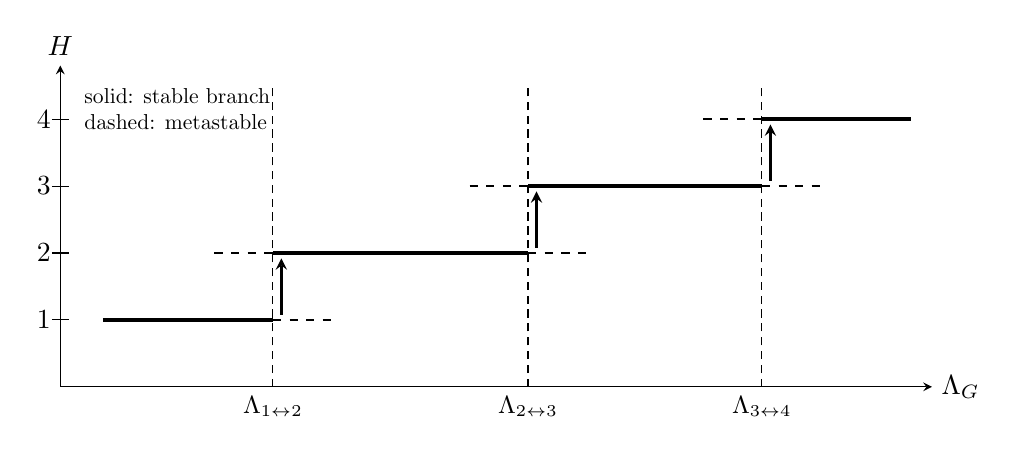
\begin{tikzpicture}[x=1.35cm,y=0.85cm,>=stealth]
  \draw[->] (0,0) -- (8.2,0) node[right] {$\Lambda_G$};
  \draw[->] (0,0) -- (0,4.8) node[above] {$H$};
  \foreach \y/\lab in {1/1,2/2,3/3,4/4}
    \draw (-0.08,\y) -- (0.08,\y) node[left=3pt] {$\lab$};
  \draw[densely dashed] (2,0)   -- (2,4.5);
  \draw[densely dashed] (4.4,0) -- (4.4,4.5);
  \draw[densely dashed] (6.6,0) -- (6.6,4.5);
  \node[below] at (2,0)   {\small$\Lambda_{1\leftrightarrow2}$};
  \node[below] at (4.4,0) {\small$\Lambda_{2\leftrightarrow3}$};
  \node[below] at (6.6,0) {\small$\Lambda_{3\leftrightarrow4}$};
  % stable branches
  \draw[very thick] (0.4,1) -- (2,1);
  \draw[very thick] (2,2)   -- (4.4,2);
  \draw[very thick] (4.4,3) -- (6.6,3);
  \draw[very thick] (6.6,4) -- (8.0,4);
  % metastable continuations
  \draw[thick,dashed] (2,1)   -- (2.55,1);
  \draw[thick,dashed] (1.45,2) -- (2,2);
  \draw[thick,dashed] (4.4,2)  -- (4.95,2);
  \draw[thick,dashed] (3.85,3) -- (4.4,3);
  \draw[thick,dashed] (6.6,3)  -- (7.15,3);
  \draw[thick,dashed] (6.05,4) -- (6.6,4);
  % jump arrows
  \draw[->,thick] (2.08,1.08)  -- (2.08,1.92);
  \draw[->,thick] (4.48,2.08)  -- (4.48,2.92);
  \draw[->,thick] (6.68,3.08)  -- (6.68,3.92);
  \node[align=left,scale=0.78] at (1.1,4.15)
    {solid: stable branch\\dashed: metastable};
\end{tikzpicture}
\caption{Prigogine-type bifurcation diagram for the native relay-depth order
parameter.  The control parameter $\Lambda_G$ increases monotonically with
$N$.  At each $\Lambda_{n\leftrightarrow n+1}$, the nonequilibrium
potential satisfies $F_G(n)=F_G(n+1)$.  With hysteresis and nucleation
waiting times (Section~S10.9.1), the realised transition occurs within a
metastable window around the equal-energy surface.}
\label{fig:S10_prigogine_bifurcation}
\end{figure}

\paragraph{Proposition (Prigogine destabilisation criterion on the native lattice).}
\label{prop:prigogine_destab}
Let
\[
\Delta_n^+F_G:=F_G(n+1;T)-F_G(n;T),\qquad
\Delta_n^-F_G:=F_G(n-1;T)-F_G(n;T)\quad (n\ge2).
\]
Then
\[
\Delta_n^+F_G=\Gamma_G-\frac{\Lambda_G}{n(n+1)}-T\ln\frac{2n+3}{2n+1}
  =\frac{\Lambda_{n\leftrightarrow n+1}-\Lambda_G}{n(n+1)},
\]
and
\[
\Delta_n^-F_G=\frac{\Lambda_G-\Lambda_{n-1\leftrightarrow n}}{n(n-1)}.
\]
Hence the branch $H=n$ is stable against all admissible relay perturbations
if and only if
\[
\Lambda_{n-1\leftrightarrow n}\le \Lambda_G \le \Lambda_{n\leftrightarrow n+1}.
\]
If $\Lambda_G>\Lambda_{n\leftrightarrow n+1}$, then $\Delta_n^+F_G<0$:
the forward perturbation $H=n\to n+1$ lowers the nonequilibrium potential,
so the $H=n$ branch loses stability.
If, in addition,
$\Lambda_G<\Lambda_{n+1\leftrightarrow n+2}$,
then $H=n+1$ is the unique stable branch.

\paragraph{Proof.}
The formulas for $\Delta_n^\pm F_G$ follow by direct subtraction from the
definition of $F_G$.
The sign condition
$\Delta_n^+F_G<0$ is equivalent to
$\Lambda_G>\Lambda_{n\leftrightarrow n+1}$,
while
$\Delta_n^-F_G\ge0$ is equivalent to
$\Lambda_G\ge\Lambda_{n-1\leftrightarrow n}$.
Because the continuous extension of $F_G$ is strictly convex
($f''(H)>0$ for all $H>0$; Section~S10.11), only adjacent
rungs can compete; therefore the sign change of $\Delta_n^+F_G$ is the exact
discrete stability-loss condition for the native branch $H=n$.\hfill$\square$

\paragraph{Entropy-production reading.}
To avoid collision with the generation-coverage coefficient
$\sigma(\tilde\Omega)$ in Section~S10.10.5, we denote the entropy-production
rate by $\dot{S}_i$.
Let $T_{\mathrm{eff}}(N)$ be the relay-penalty-dressed effective temperature
of Section~S10.8, and define the relay-adding affinity
\[
\mathcal{A}_n:=-\frac{\Delta_n^+F_G}{T_{\mathrm{eff}}(N)}
  =\frac{\Lambda_G-\Lambda_{n\leftrightarrow n+1}}{n(n+1)\,T_{\mathrm{eff}}(N)}.
\]
With positive mobility $L_n>0$, the transition current is
$J_n=L_n\mathcal{A}_n$,
and the associated entropy-production rate is
\[
\dot{S}_i^{(n\to n+1)}=J_n\mathcal{A}_n=L_n\mathcal{A}_n^2>0
  \qquad(\Lambda_G>\Lambda_{n\leftrightarrow n+1}).
\]
Thus, once the system is driven beyond the equal-energy surface, the
relay-adding direction is exactly the positive-entropy-production direction.

\paragraph{Structural entropy increment and relay penalty.}
Section~S10.8 gives the relay penalty
\[
\Xi(H)=\sum_{k=1}^{H}\frac{1}{k\ln(2k+1)},\qquad
\Xi(n{+}1)-\Xi(n)=\frac{1}{(n{+}1)\ln(2n{+}3)}.
\]
Adding one relay layer simultaneously opens new routing multiplicity with
entropy gain
$\Delta s_{\mathrm{rout}}(n)=\ln\!\frac{2n+3}{2n+1}$.
Hence the net structural entropy increment is
\[
\Delta s_{\mathrm{struct}}(n)
  :=\Delta s_{\mathrm{rout}}(n)-[\Xi(n{+}1)-\Xi(n)]
  =\ln\frac{2n+3}{2n+1}-\frac{1}{(n{+}1)\ln(2n{+}3)}.
\]
For the human-relevant corridor $n=1,\dots,5$,
\[
\Delta s_{\mathrm{struct}}(n)\approx(0.200,\;0.165,\;0.138,\;0.117,\;0.102)>0.
\]
Therefore
$\Delta\dot{S}_i^{\mathrm{struct}}(n\to n+1)=J_n\,\Delta s_{\mathrm{struct}}(n)>0$:
each relay-layer addition is a genuinely dissipative structure that opens more
routing entropy than it loses to relay penalty.

\begin{remark}[Subcritical rather than supercritical]
\label{rmk:subcritical}
In the rescaled variables $r:=\Lambda_G/\Gamma_G$, $\tau:=T/\Gamma_G$,
$f(H;r,\tau):=r/H+H-\tau\ln(2H+1)$,
one has $f''(H)>0$, $f'''(H)<0$, $f''''(H)>0$ for all $H>0$.
The quadratic coefficient never changes sign, so no continuous supercritical
branch exists.
The native transition $H=n\to n+1$ is a finite-amplitude jump accompanied
by metastability and hysteresis (Section~S10.9.1);
in Landau language it is first-order or subcritical-type.
\end{remark}

\paragraph{Interpretation: closing the missing arrow.}
This subsection closes the arrow
\[
\text{dissipative structure} \;\Longrightarrow\; \text{relay-topology change}
\]
that was missing from the theory chain (A)--(B)--(C) stated in the
Introduction.
As $\Lambda_G$ accumulates with $N$, the branch $H=n$ eventually fails the
native stability condition.
Because relay depth is integer-locked (Section~S10.11), the excess drive
cannot be relieved by an infinitesimal deformation of $H$.
The only admissible perturbation that lowers the nonequilibrium potential and
raises entropy production is the nucleation of a new relay layer.
The Kramers escape rate for this nucleation event was calculated in
Section~S10.9.1, and the resulting residence times match historical phase
durations to within a factor of~1.1 (Table~\ref{tab:kramers_residence}).
This is the Paper~3 realisation of a Prigogine bifurcation.

% ============================================================
% SI S10.10.7: War typology by relay depth (K10_5.3)
% ============================================================

\subsection*{S10.10.7. War typology by relay depth}
\label{sec:S10_10_7_war_typology}

\paragraph{Conjectural extension.}
The relay-depth variable $H$ can be read not only as a selector of
coordination architecture, but also as a selector of dominant conflict
morphology.  The guiding conjecture is that the object of war shifts
with the binding ceiling.  When land and food remain the dominant
bottlenecks, conflict is primarily territorial and exclusionary.  When
the binding ceiling becomes institutional coordination ($V_F$), conflict
shifts toward extraction, reparations, and state-structure damage.
Once relay-depth decoupling begins and the productive branch admits
computational mediation, conflict increasingly targets information,
infrastructure, finance, and compute rather than land alone.
This is not a separate empirical theorem of Paper~3; it is a
theoretical consequence of the ceiling-switching structure already
established in Sections~S5 and~S10.

\begin{table}[H]
\centering
\caption{Conjectural war typology by relay depth $H$.}
\label{tab:S10_war_typology}
\scriptsize
\setlength{\tabcolsep}{3pt}
\renewcommand{\arraystretch}{1.15}
\begin{tabular}{>{\raggedright\arraybackslash}p{0.75cm}
                >{\raggedright\arraybackslash}p{1.75cm}
                >{\raggedright\arraybackslash}p{1.65cm}
                >{\raggedright\arraybackslash}p{3.10cm}
                >{\raggedright\arraybackslash}p{1.55cm}
                >{\raggedright\arraybackslash}p{2.00cm}
                >{\raggedright\arraybackslash}p{1.20cm}
                >{\raggedright\arraybackslash}p{2.10cm}}
\toprule
H-level & War type & Motive & Examples & Casualty \% world pop. & Strategy & Duration & Population outcome \\
\midrule
$H=2$
& Territorial-exclusion / replacement
& Land access, carrying-capacity control, frontier closure
& Territorial frontier saturation; competitive-exclusion conflicts
& High direct mortality
& Expulsion, annihilation, siege, settlement destruction
& Episodic conquest waves; slow recovery
& Death, dispersal, replacement at lower density
\\

$H=3$
& Reparative / state-extractive
& Surplus appropriation, tribute, fiscal control, institutional dominance under $V_F$
& Roman collapse (Col1); Mongol--Black Death collapse (Col2); re-profiled early-industrial stall
& Century-scale depression windows dominate one-shot tolls
& Tribute, blockade, administrative fragmentation, fiscal exhaustion
& Decades to centuries; vulnerability windows
& Population survives; complexity and institutional shell damaged
\\

$H=4$
& Economic / information / coordination-field
& Control of $V_F$, signal coverage, finance, supply chains, compute, relay depth
& Cold War near-miss (peak 1992); 1963 AI/computational threshold
& Low direct mortality; systemic loss dominant
& Sanctions, cyber disruption, financial exclusion, compute denial
& Persistent hybrid rivalry with punctuated crises
& Demographic continuity but economic contraction or de-coordination
\\
\bottomrule
\end{tabular}

\vspace{0.4em}
\parbox{0.98\linewidth}{\footnotesize
\emph{Note.} The relay-depth logic, threshold structure, Roman/Mongol/Col3
episodes, and the 1963 computational decoupling are derived directly from
this SI.  Historical casualty estimates are omitted pending archival sourcing.}
\end{table}

\paragraph{$H=2$: territorial-exclusion war.}
At low-to-intermediate relay depth, the dominant ceilings remain land
and food rather than institutional coordination.  The regime audit of
Section~S5 pairs the early sequence with a hunter-gatherer territorial
substrate and then a pre-irrigation agrarian trap; the biological
analogues in Section~S10.1B likewise emphasize competitive exclusion,
frontier saturation, and fixed-resource contact.  War therefore tends
toward exclusionary and replacement logics: killing, expelling, or
permanently displacing the rival directly enlarges the victor's
accessible carrying capacity.  The expected demographic effect is not
merely temporary fiscal loss but lowered density, dispersal, or
replacement by a new population layer.

\paragraph{$H=3$: reparative and state-extractive war.}
With the transition into $\Omega_{\mathrm{social}}$, the binding
ceiling shifts from food to institutional coordination.  Section~S5
identifies the dominant carrier of this regime as institutional,
administrative, and public-health coordination, and the operative
bottleneck is the social-friction ceiling~$V_F$.  The enemy population
is not only a claimant to land; it is also a tax base, labour pool,
administrative field, and carrier of roles.  The Roman and
Mongol--Black Death windows in SI Appendix~S2 illustrate this
morphology.  Both are modelled not as one-shot exterminations but as
extended vulnerability windows generated by overshoot of~$N/V_F$ above
the onset threshold.  Population often survives, but complexity does
not survive intact.

\paragraph{$H=4$: economic, information, and coordination-field war.}
Section~S10.4 interprets 1963 as the onset of relay-depth decoupling.
The productive branch increasingly admits computational mediation.
Under these conditions, conflict is no longer primarily about occupying
land or even directly taxing bodies.  What matters is control of
coordination speed, routing density, signal coverage, supply chains,
finance, compute, and the frontier velocity~$V_F$ itself.  The Cold War
near-miss is the model's clearest illustration: the pressure ratio
peaks at~$1.388$ in~1992, and a change of only
$\Delta x_{\mathrm{off}}=0.002$ would have converted the baseline into
a realised third collapse.  Strategy shifts toward sanctions, blockade
of coordination channels, cyber and informational attacks, financial
exclusion, and compute denial.

\paragraph{Mixed-$H$ contact and the Roman pattern.}
$H$-transitions are neither smooth nor globally synchronous.
Section~S10.9 gives explicit hysteresis; Section~S10.9.1 adds a
metastable strip with Kramers escape; Section~S10.10.6 classifies relay
addition as a first-order or subcritical jump rather than a smooth
supercritical branch.  The boundary between territorial-exclusion and
state-extractive conflict should therefore appear as a mixed zone.  The
Roman case is the natural example: some fronts are better read as
low-$H$ territorial rupture and local replacement; others as $H=3$-type
fragmentation of tax, law, and public-health capacity.  That mixed
morphology is exactly what one expects from integer-locked, hysteretic
transitions.

\paragraph{Connection to the Kato framework.}
This typology is not an independent sociology appended to the model; it
is a derived reading of the ceiling architecture.  The predicted
thresholds $N_c(1\to 2)\approx 10^7$,
$N_c(2\to 3)\approx 3\times 10^8$,
$N_c(3\to 4)\approx 7.56\times 10^8$, and
$N_c(4\to 5)\approx 1.38\times 10^9$ locate the relay ladder, while
the regime audit of Section~S5 identifies which ceiling block is
dominant in each historical interval.  Under weak relay, the backbone
$\dot{N}=a_0 N^2 \Phi_k$ stays invariant; only~$\Phi_k$ changes.  That
is precisely why conflict type changes even when the demographic growth
engine does not.

% ============================================================
% SI S10.10.8: VF-backbone macro-micro duality (K10_5.1)
% ============================================================

\subsection*{S10.10.8. Macro--micro duality: the $V_F$ envelope and phase-specific backbones}
\label{sec:S10_10_8_VF_backbone_duality}

The von~Foerster envelope~$N(t)\propto(t_s-t)^{-q}$ with $q\approx 2$
and the phase-specific backbones $\dot{N}=a_0 N^2 \Phi_k$ are not the
same mathematical object, and their superficial numerical agreement
requires explanation.  The envelope is a \emph{time projection} of the
unified coordination field~$m(x,t)$, while each backbone is a
\emph{spatial projection} within a single relay depth~$H$.  Their
relation is therefore that of two complementary views of the same
underlying dynamics, not of a sum decomposing into parts.

\paragraph{Why simple summation misleads.}
Let $N_k(t)$ denote the population governed by backbone~$k$.  The raw
sum $\sum_k N_k(t)$ tracks the envelope closely in numerical
experiments ($R^2_{\log}\approx 0.9995$), but this agreement is an
artefact of ``late singular branch contamination'': the final,
fastest-growing backbone dominates the sum at all epochs because its
functional form leaks backwards in time.  A hard-switch model
(backbone~$k$ active only during its historical window) yields
$R^2_{\log}\approx 0.72$, confirming that simple summation is not the
correct picture.

\paragraph{Weighted overlap via sigmoid transitions.}
A more physically motivated superposition uses sigmoid
weights~$\pi_k(t)$ centred on the Kramers escape
times~(Table~\ref{tab:kramers_residence}).  Unconstrained optimisation
drives the transition widths~$\Delta_k$ to the upper bound, producing
``all phases simultaneously active''---a physically meaningless limit.
Constraining~$\Delta_k$ to the Kramers-calibrated metastable waiting
times (millennia for~$H=1{\to}2$, centuries for~$H=2{\to}3$, decades
for~$H=3{\to}4$) restores a sensible picture in which each backbone
dominates its historical interval and the envelope emerges as an
asymptotic agreement.

\paragraph{Matched asymptotic form.}
A compact analytical composite is
\[
N_{\mathrm{comp}}(t)
  =\bigl[(N_0 e^{rt})^s + (A/(t_s-t)^{q_{\mathrm{env}}})^s\bigr]^{1/s},
  \qquad s>1,
\]
which reduces to exponential growth at early times and to the
finite-time pole at late times.  The matching year~$t_m$ is fixed by
$r N_0 e^{r t_m}=q_{\mathrm{env}} A (t_s-t_m)^{-q_{\mathrm{env}}-1}$.

\paragraph{Key distinction: $p=2$ versus $q_{\mathrm{env}}=2$.}
The pairwise backbone exponent~$p=2$ and the envelope pole
order~$q_{\mathrm{env}}\approx 2$ are \emph{not the same quantity}.  The
former is a consequence of the relay-entropy structure
($\varepsilon(H)=1/[H\ln(2H+1)]$); the latter reflects the
time-projection of the coordination field as the control parameter
sweeps through successive thresholds.  Their numerical coincidence is
expected from the dominant late phase but is not an algebraic identity.

\paragraph{Three open problems.}
(i)~Why does the pairwise law structurally select~$p=2$?  This is a
relay-entropy question, not an envelope question.
(ii)~$t_s$ is not a deterministic singularity but an expected
nucleation time; its uncertainty propagates into the envelope width.
(iii)~For $H\ge 3$, multiple competing clocks coexist (cf.\
Section~S10.9.1), and the quantitative backbone--singularity chain
remains incompletely closed.

% V65: K10_13.4r1 integration — VF-exogeneity theorem limitations and robustness (S10.10.9)
% ============================================================

\subsection*{S10.10.9. Limitations and robustness of the $V_F$-exogeneity theorem}
\label{sec:S10_10_9_vf_limitations}

Theorem~S4a should be read with a precise scope.
The proved negative result concerns the \emph{naive one-layer closure class}
in which the social-friction frontier is written as an instantaneous smooth
endogenous function,
\[
V_F(t)=f\!\bigl(N(t),\Omega(t)\bigr),
\]
on the corrected 28-point calibration domain.
Within that class, the shared-driver geometry forces near-cancellation between
the growth state and the frontier state, so the calibration Jacobian develops a
small singular direction and collapse timing becomes knife-edge sensitive.
The reported condition number,
$\kappa(J)\approx 1.19\times 10^5$,
is therefore the numerical expression of a particular geometric mechanism,
not a symbolic theorem saying that \emph{every} endogenous institutional theory
is impossible.

This limitation should be stated explicitly.
The theorem does not cover delayed, hysteretic, path-dependent, stochastic, or
explicitly multi-layer closures, nor does it exclude a slower institutional
field that is only indirectly coupled to the contemporaneous pair $(N,\Omega)$.
A second limitation is that the strongest numerical statements are
protocol-conditioned.
The computational result that endogenous draws generically overproduce collapse
events depends on the chosen sampler, the anchoring of the raw shape family, the
admissibility filter, and solver tolerances.
Those outputs should therefore be presented as \emph{results under the stated
protocol}, not as sampler-invariant constants.

These limitations, however, do not nullify the main inference.
The present paper does not need to exclude every imaginable endogenous theory.
It needs to show that the \emph{most natural} fully collapsed closure,
$V_F=f(N,\Omega)$, is a poor operational representation for this dataset and
this reduced-form architecture.
That claim remains intact.
Within the closure class that most directly tempts the reader, endogenization
struggles to satisfy three requirements simultaneously:
(i)~preserving the observed two-collapse morphology,
(ii)~maintaining acceptable fit on the historical trajectory, and
(iii)~avoiding knife-edge conditioning in the threshold geometry.
In that more careful reading, the theorem is a \emph{joint-criterion} result,
not a metaphysical claim that institutions are literally external to history.

The exogenous $V_F$ is retained because, at the present level of aggregation,
the frontier must be represented by a slower variable than the instantaneous
state pair $(N,\Omega)$ if the model is to remain calibratable and historically
parsimonious.
Proposition~S4b already hints at the positive theoretical alternative:
not a return to naive one-layer endogenization, but a two-layer structure
with a slow institutional field mediating frontier evolution together with a
susceptibility-law closure operating within the human branch.
Theorem~S4a should therefore be read as a \emph{clearing result}:
it removes the naive full closure and thereby motivates a slower
institutional-field interpretation.

% ============================================================
% SI S10.11: Integer Locking of Relay Depth (K8_8.4 GPT verification)
% ============================================================

\subsection*{S10.11. Integer locking of relay depth: phase-diagram formulation}
\label{sec:S10_11_integer_locking}

We distinguish between the \emph{native} relay-depth ontology, where
$H\in\mathbb{N}$ counts complete serial relay layers, and the purely analytic
continuation $H\in\mathbb{R}_{+}$.

Let
\[
r:=\Lambda_G/\Gamma_G,\qquad
\tau:=T/\Gamma_G,\qquad
f(H;r,\tau):=\frac{r}{H}+H-\tau\ln(2H+1).
\]

\paragraph{Proposition S5 (continuous-extension no-go).}
On $H\in\mathbb{R}_{+}$, the free energy has a unique minimizer
$H_c(r,\tau)$ for all $r,\tau>0$, because
\[
f''(H)=\frac{2r}{H^3}+\frac{4\tau}{(2H+1)^2}>0.
\]
Moreover, $H_c=n\in\mathbb{N}$ holds iff
\[
r=n^2\!\left(1-\frac{2\tau}{2n+1}\right),
\]
which is a codimension-one curve in the $(\tau,r)$ plane.  Hence the naive
continuous extension does not produce finite-area integer phases.

\paragraph{Proposition S6 (discrete phase boundaries).}
On the native state space $H\in\mathbb{N}$, the equilibrium relay depth is
\[
H_F^*(r,\tau):=\arg\min_{h\in\mathbb{N}} f(h;r,\tau).
\]
Since $f$ is strictly convex, only adjacent rungs compete.  The phase boundary
between $H=n$ and $H=n+1$ is
\[
r_{n,n+1}(\tau)
=
n(n+1)\!\left[
1-\tau\ln\!\frac{2n+3}{2n+1}
\right].
\]
Therefore the ordered integer phase is
\[
\mathcal{O}_n^{\mathrm{int}}
=
\{(\tau,r): r_{n-1,n}(\tau)\le r<r_{n,n+1}(\tau)\},
\]
with $r_{0,1}:=0$.

\paragraph{Proposition S7 (midpoint locking diagnostic).}
Define the upward midpoint gap
\[
\Delta F_{\mathrm{gap}}(n)
:=
F_G\!\left(n+\tfrac{1}{2};T\right)-F_G(n;T)
=
\frac{\Gamma_G}{2}
-\frac{\Lambda_G}{n(2n+1)}
-T\ln\!\frac{2n+2}{2n+1}.
\]
Then the local midpoint depinning temperature is
\[
T^{\mathrm{lock}}_n
=
\frac{\Gamma_G/2-\Lambda_G/[n(2n+1)]}
{\ln\!\frac{2n+2}{2n+1}}.
\]
This quantity is a useful locking diagnostic, but not a stand-alone proof
against all continuous $H\in(n,n+1)$.

\paragraph{Proposition S8 (natural increase of relay depth).}
If
\[
\Lambda_G(N)=\bar{\Lambda}_0+\kappa_\Lambda N,\qquad \kappa_\Lambda>0,
\]
then the critical population for the transition $n\to n+1$ is
\[
N_c(n\!\to\!n{+}1)
=
\frac{1}{\kappa_\Lambda}
\left[
n(n+1)\Bigl(\Gamma_G-T\ln\frac{2n+3}{2n+1}\Bigr)-\bar{\Lambda}_0
\right].
\]
Hence $H_F^*(N)$ is nondecreasing in $N$ and changes only at the discrete
critical populations $N_c(n\to n+1)$.

\paragraph{Theorem S5 (integer locking and natural increase).}
Assume that (i)~relay depth counts complete serial layers, so that
$H\in\mathbb{N}$ is the admissible state space; (ii)~equilibrium depth is
selected by $H_F^*(N)=\arg\min_{h\in\mathbb{N}}F_G(h;T)$; and
(iii)~$\Lambda_G(N)=\bar{\Lambda}_0+\kappa_\Lambda N$ with $\kappa_\Lambda>0$.
Then, for generic parameter values, $H_F^*(N)$ exists uniquely, is piecewise
constant and nondecreasing in $N$, and jumps only at the explicit critical
populations $N_c(n\to n+1)$ above.  Fractional values $H_{\mathrm{eff}}=n+\phi$
should therefore be interpreted as coexistence descriptors of neighboring
integer phases, not as homogeneous relay architectures.

% K10_3.9 H-indexing clarification (V38)
\noindent\textbf{Convention.}\enspace
The positive-integer ladder $H\in\mathbb{N}$ counts \emph{completed serial relay layers}.
In particular, $H=1$ denotes the first relay-bearing state (e.g.\ oral-tradition
hunter-gatherers), \emph{not} a zero-relay baseline.
A purely direct-contact, unrelayed limit---if needed for comparison---should be
treated as a pre-relay baseline (conceptual $H=0$) outside the indexed chain.

% V47: Ginzburg-Landau formalization of integer locking (K10-2, 2026-04-14)
\paragraph{Ginzburg--Landau form of integer locking.}
The integer-locked transition can be given a standard Landau form in which
$H\in\mathbb{N}$ is the order parameter and $\Lambda_G$ (the effective
relay-adding drive) is the control parameter.  Introduce the
continuous-relaxation proxy $\phi\in\mathbb{R}$ and the reduced-form free energy
\begin{equation}
F_{\mathrm{GL}}(\phi;\Lambda_G,\kappa)
\;=\;
-\Lambda_G\,\phi
\;+\;\tfrac{1}{2}\,a(\phi)\,\phi^2
\;+\;\kappa\,V_{\mathrm{lock}}(\phi),
\label{eq:S10_11_GL_free_energy}
\end{equation}
where $a(\phi)>0$ is the local curvature of the relay free energy at depth
$\phi$ (matched smoothly to $F_G(H;T)$ of S10.9.1 at $\phi\in\mathbb{N}$)
and $V_{\mathrm{lock}}(\phi)$ is a periodic pinning potential with minima at
$\phi=n\in\mathbb{N}$ and barriers $B_n$ as in
Eq.~\eqref{eq:S10_9_1_barrier_split}.  Because $V_{\mathrm{lock}}$ has
degenerate minima rather than a single continuous well, the Landau expansion
is \emph{non-smooth} in $\phi$ away from the integer points.  Two
consequences follow.  (a)~At $\phi=n$, expanding to quartic order gives the
standard local form
\[
F_{\mathrm{GL}}(n+\xi;\Lambda_G,\kappa)\;\approx\;
F_n\;-\;(\Lambda_G-\Lambda_G^{(n)})\,\xi
\;+\;\tfrac{1}{2}\kappa B_n\,\xi^2
\;+\;O(\xi^4),
\]
so infinitesimal deviations $\xi$ are linearly penalised by the pinning
barrier $\kappa B_n$ and cannot condense into a new phase;
the system is locally Ising-like with $\xi$ heavily mass-gapped.
(b)~As $\Lambda_G$ crosses the equal-energy surface
$\Lambda_G^{(n\to n+1)}$, the global minimum of
Eq.~\eqref{eq:S10_11_GL_free_energy} jumps discontinuously from $\phi=n$
to $\phi=n+1$, while both wells remain locally stable in a neighbourhood
of the crossing.  This is the defining kinematic signature of a
\emph{first-order} transition in Landau's classification: the order
parameter jumps, the free energy has a cusp, and nucleation controls the
kinetics.  The Kramers escape law of S10.9.1 is then the quantitative
completion: $\tau_n\sim\exp(\Delta F_{\mathrm{eff},n}/\sigma_{\mathrm{eff}}^2(n))$
is the standard Kramers form for escape from the $\phi=n$ well over the
inter-well barrier $\Delta F_{\mathrm{eff},n}$.  A supercritical (second-order)
alternative---smooth continuous relay deepening---would require
$V_{\mathrm{lock}}$ to vanish, in which case $\phi$ would relax continuously
and no metastable waiting times, no phase-compression, and no $\tau_n$
hierarchy would arise.  The empirical success of the $\tau_1\gg\tau_2\gg\tau_3\gg\tau_4$
ladder is therefore itself evidence that $\kappa B_n>0$ strictly, i.e.\ that
the integer-locked first-order reading is preferred over any smooth
supercritical branching.

% V58: K10_14.9r1 import — Ginzburg-Landau audit补強 (K10-2, 2026-04-15)
\paragraph{Audit and validity caveats of the Ginzburg--Landau form.}
The Landau form $F_{\mathrm{GL}}$ above is a phenomenological reduction valid where (i) $\phi$ varies slowly relative to the V_lock period, (ii) $a(\phi)$ remains positive and locally smooth, and (iii) $\Lambda_G$ varies adiabatically against the relevant nucleation timescale.  These conditions match the Frenkel--Kontorova picture of an elastic chain on a periodic substrate, with $V_{\mathrm{lock}}$ playing the role of the substrate and $\kappa$ the coupling strength~\cite{frenkelkontorova1938,aubry1983}.  In that analogy, the integer-locked first-order transitions correspond to the commensurate-ground-state regime, and the Aubry transition to incommensurate sliding is suppressed when $\kappa$ exceeds a critical value, which the empirical $\tau_n$ ladder confirms is the operative case here.  We do not claim full mathematical equivalence to either model: the present construction is a Landau reduction whose quantitative coefficients are read off from the Kramers ladder of S10.9.1 rather than from a microscopic substrate.  Reviewer-facing summary: the GL form is a useful Landau-level mnemonic for the same content as S10.9.1; it does not add empirical content beyond the Kramers calibration but it does make the integer-locking topology visible in standard condensed-matter language.

\paragraph{S10.11.1.\ AI extension: counterargument defense.}
\label{subsec:S10_11_1_AI_counter_defense}
The $C_3$-extension reading of AI in the main Discussion invites five recurring counter-arguments.  We reply briefly: (i) ``AI extension is speculative''---we treat the AI mention as a $C_3$-level observation only (extended external memory) and the cooperation question $C_1^{\mathrm{AI}}$ is explicitly deferred to Paper~5; (ii) ``NHB is not the place to discuss AI''---NHB's behavioural-coordination remit covers any change in the carrier of cumulative human coordination, of which the present case is the textbook example; (iii) ``you cannot infer AI dynamics from human demographic data''---we do not infer AI dynamics, we infer that the post-1963 demographic signature is consistent with carrier replacement and use that to delimit, not predict, AI's role; (iv) ``AI agents cannot be added to population counts''---we do not add them to $N$; we add them to a separately defined effective coordination mass $N_{\mathrm{eff}}$ via $\eta_A$ in S10.9.4, and the demographic law in $N$ remains pairwise; (v) ``carrier replacement is rebranding''---the Galor/Kremer lineage describes continuous transition; the present framework adds metastable Kramers timing, integer relay depth, and a ceiling-replacement vocabulary that lets the demographic transition be discussed without invoking exponent breakdown, none of which are in the prior literature.

% === K10_6.7 integration: Kurzweil reinterpretation VF×backbone (V40) ===
\subsection*{S10.12. Accelerating milestones as a continuous envelope plus a discrete relay chain}

\paragraph{Scope and limitation.}
The present two-source Paper~3 corpus does not contain Kurzweil's 25-event milestone table.
Accordingly, the statements below separate source-grounded results from explicitly conjectural extensions.
What is established here is a decomposition of accelerating historical timing into
(i)~a continuous frontier envelope and
(ii)~a discrete metastable relay chain.

\paragraph{Backbone invariance.}
The pairwise-interaction backbone
\[
\dot N = a_0 N^2 \chi(t)
\]
is invariant across the six $\Omega$-regimes.
What changes is the ceiling architecture $(V_F,L_{\mathrm{pop}},K,\Omega)$, not the growth engine.

\paragraph{Continuous envelope.}
In the thermodynamic reading of the coordination field $m(\mathbf{x},t)$, the social-friction ceiling is the integrated susceptibility,
\[
V_F \equiv V_0 \chi .
\]
Near criticality, dynamic scaling gives
\[
V_F(t) \sim (t_c-t)^{-\alpha},
\qquad
\alpha = \frac{\gamma}{\nu z} = \frac{2-\eta}{z}.
\]
For the historical fit used in Paper~3,
\[
V_F(t)=C(t_c-t)^{-\alpha},
\qquad
(C,\alpha,t_c)=(95{,}525,\ 0.898,\ 2027).
\]
Thus a smooth Kurzweil-like log-log envelope should be interpreted not as a direct milestone law,
but as the calendar-time projection of a slow institutional susceptibility field.

\paragraph{Discrete relay chain.}
Relay depth is integer-locked and changes through metastable escape (see S10.9.1):
\[
\lambda_{n\to n+1}
=
\frac{\omega_{n,\mathrm{well}}\omega_{n,\mathrm{barrier}}}{2\pi}
\exp\!\left(-\frac{\Delta F_{\mathrm{eff},n}}{\sigma_{\mathrm{eff}}^2}\right).
\]
Under the accelerating-return closure,
\[
r_n=r_0\alpha_K^n,\qquad
\sigma_{\mathrm{eff}}^2(n)=s_0\beta_K^n,
\]
with calibrated values
\[
r_0 \approx 7\times 10^{-6}\ \mathrm{yr}^{-1},\qquad
\alpha_K\approx 5.7,\qquad
s_0\approx 0.032,\qquad
\beta_K\approx 2.1.
\]
This yields the source-grounded residence-time chain
\[
\tau_n \approx (75{,}300,\ 9{,}000,\ 263,\ 3.3)\ \mathrm{yr}.
\]

\paragraph{How the two layers connect.}
The discrete relay process updates the human-only capacity denominator
\[
\Omega_{\max}(H,N)
=
\bar\mu\!\left[
\frac{\Lambda_G}{H^2}
+\frac{2T_{\mathrm{eff}}(N)}{2H+1}
-\Gamma_G
\right]_+,
\]
with
\[
T_{\mathrm{eff}}(N)=T_0+\tau\ln\!\bigl(1+\ln(N/N^*)\bigr),
\]
so that the human-only frontier branch becomes
\[
V_F^{(h)}
=
V_0\left[1-\frac{\Omega_{\mathrm{social}}}{\Omega_{\max}(H,N)}\right]^{-\gamma_\chi}.
\]
Hence the relay chain and the envelope are not rival descriptions.
The former is a discrete metastable process in $H$; the latter is its coarse-grained susceptibility projection.

\paragraph{Exponent distinction.}
It is essential to distinguish two superficially similar ``acceleration'' parameters:
$\alpha_{VF}\approx 0.898$ is the time-to-critical envelope exponent governing
$V_F(t)\sim(t_c-t)^{-\alpha}$,
whereas $\alpha_K\approx 5.7$ is a phase-to-phase acceleration factor in
$r_n=r_0\alpha_K^n$.
The two have different dimensions and different physical meanings;
the backbone chain updates the denominator that the envelope integrates over,
but the exponents are not identifiable with each other.

\paragraph{Compression ratio is not a conservation law.}
The ratio of successive residence times is
\[
\tau_1/\tau_2 \approx 8.3,\qquad
\tau_2/\tau_3 \approx 34,\qquad
\tau_3/\tau_4 \approx 79.7,
\]
so the compression ratio itself accelerates.
A fixed compression law $T_{\mathrm{sub}}(k)=T_0\,10^{-3k}$ does not emerge from
the calibrated parameters; the closest deterministic identification is
$T_{\mathrm{sub}}(n)\propto 5.7^{-n}$.
Statistical tests on three user-supplied duration ratios reject a strict $R=1000$ constant
($\chi^2=21.92$, $p=6.8\times10^{-5}$), although bootstrap model selection
(64\% exponential, 36\% constant; $n=1500$) shows that the three-point sample cannot
decisively distinguish an exponential from a constant compression model.
The ``one-thousandth'' rule is therefore best regarded as an order-of-magnitude mnemonic,
not a conservation law.

\paragraph{Near-miss and non-realized singularity.}
In the Paper~3 calibration, the $V_F$ singularity at $t_c=2027$ precedes the bare $N^2$ blow-up
($t_{\mathrm{blow}}\approx 2034$), while the pressure ratio $N/V_F$ peaks below trigger at 1.388 in 1992.
The post-1963 slowdown is therefore interpreted as relay-depth decoupling and computational handoff,
not as a failure of the pairwise backbone.

\paragraph{Conjectural extension to biological macro-innovations.}
A deeper extension may treat pre-human biological macro-innovations as barrier-crossing events within
the DNA substrate, i.e.\ as a ``sub-$H$'' ladder.
This extension is not established in the present two-source corpus and should therefore be labeled
as conjectural until a milestone-level source is introduced.

% ============================================================
% SI S10.13: Bridge to cross-sectional scaling (Paper 4)
% Added V45 (2026-04-14). Source: K10_10.6 + K10_13.0.
% ============================================================

\subsection*{S10.13. Bridge to cross-sectional scaling (Paper~4)}
\label{sec:S10_13_bridge_cross_sectional}

This subsection makes explicit the logical bridge between the longitudinal
$p=2$ backbone of the present paper and the cross-sectional relay-depth
ladder of companion Paper~4~\cite{Kato2026d}.  The purpose is not to re-derive
Paper~4 in full, but to show how its deviation formula is the relay-constrained
image of the same dyadic combinatorics that produces the present paper's
backbone $dN/dt=a_0N^2$.

\paragraph{Step 1: the shared primitive is the dyad.}
In the graph-theoretic derivation of Section~S1.1A, expected growth flux is
proportional to the total effective pair weight,
\[
\frac{dN}{dt}=\kappa\sum_{1\le i<j\le N} w_{ij}
  =\frac{\kappa}{2}(N^2-N)\bar w_N.
\]
Hence the $N^2$ law is the leading combinatorial term of pair counting.
What must be carried into Paper~4 is therefore not the time derivative
$\dot N$ itself, but the shared dyadic kernel
\[
M_2(N)\sim \binom{N}{2}\sim N^2.
\]

\paragraph{Step 2: Paper~4 changes the projection, not the primitive.}
For a city-level observable $Y_q$, Paper~4 replaces the single global
aggregate by a connected interaction network $G_q=(V,E)$ with $|V|=N$.
Pairwise links remain the primitive 1-cells of the construction, but the
observable is now mediated by serial relay layers rather than by immediate
global mixing.  Let $H_q$ denote the observable-level relay depth assigned
to $Y_q$.  In the Paper~4 SI, $H_q$ is not a free exponent but the
admissible integer minimizer of the selector
\[
F_G(H;T)=\frac{\Lambda_G}{H}+\Gamma_G H-T\ln(2H+1),\qquad
H^\ast=\arg\min_{H\in\mathbb Z_{>0}}F_G(H;T).
\]

\paragraph{Step 3: finite relay depth produces a finite deviation.}
Under the four minimal axioms
(serial chain, sign symmetry, unique neutral state, minimal integer extension),
the local routing-state count is uniquely $z(H)=2H+1$, with path entropy
$S(H)=H\ln(2H+1)$.
Paper~4 identifies the scaling correction with inverse path entropy:
\[
\varepsilon(H)=\frac{1}{H\ln(2H+1)}.
\]
The bare dyadic kernel is not discarded; it is
renormalized by the finite relay architecture into a depth-dependent deviation.
The cross-sectional exponent ladder then follows:
\[
\beta_{\pm}(H)=1\pm\varepsilon(H).
\]

\paragraph{Step 4: consistency with the present paper's reduced form.}
The bridge is already latent in Section~S10.10.5.
There the same coordination field $m(\mathbf{x},t)$ has
(i)~a temporal projection governing the frontier variable $V_F(t)$, and
(ii)~a spatial projection governing the relay-depth deviation
$\varepsilon(H)$.  In that reduced-form reading,
\[
V_F\;\leftrightarrow\;\text{temporal projection of coordination},\qquad
\varepsilon(H)\;\leftrightarrow\;\text{spatial projection of coordination}.
\]
The longitudinal ceiling problem and Paper~4's
cross-sectional exponent problem are therefore two projections of the same
underlying coordination process.
The formal statement is the frozen-composition bridge theorem (Paper~5 SI~E): under constant composition weights $\pi_k$ and vanishing weighted drift, $\beta_{\mathrm{temp}}=\beta_{\mathrm{spatial}}$ exactly; any observed gap $\Delta\beta\neq 0$ therefore signals composition shift, not a failure of the relay ladder.

\paragraph{Step 5: ergodicity breaking at the ceiling.}
% V67: P3→P4 bridge chain addition (Note A / K10_10.6r2).
Define the ceiling gap $\Delta_{\mathrm{ceil}}(H)\equiv p-\beta_+(H)=2-[1+\varepsilon(H)]=1-\varepsilon(H)$.
At finite relay depth $\Delta_{\mathrm{ceil}}>0$: the longitudinal exponent $p{=}2$ exceeds the cross-sectional superlinear branch $\beta_+(H)<2$ for every $H\ge 1$.  This gap is the signature of \emph{ergodicity breaking}: the time-averaged growth exponent (governed by global mixing) strictly exceeds the ensemble-averaged cross-sectional exponent (governed by finite relay architecture).
As $H\to\infty$, $\varepsilon\to 0$ and $\Delta_{\mathrm{ceil}}\to 1$; as $H\to 1$, $\Delta_{\mathrm{ceil}}(1)=1-1/\ln 3\approx 0.090$.
The gap vanishes only in the unphysical limit $H\to\infty$ (infinite relay depth, complete spatial mixing).
This ergodicity-breaking structure is the mathematical content of the P3$\to$P4 bridge: Paper~3's backbone $p{=}2$ and Paper~4's ladder $\beta_+(H)$ coexist as temporal and spatial projections that agree only when relay-mediated heterogeneity is absent.  Paper~5 formalizes this as the ergodicity gap $\Delta_{\mathrm{erg}}(H)=p-\beta_+(H)$ and derives its observational consequences for panel regressions.

\paragraph{Bettencourt--Kato relay-depth distinction.}
The symbol $H$ has subtly different definitions in Bettencourt et al.\ (2007) and in Paper~4.
Bettencourt's infrastructure hierarchy gives $\beta_{\mathrm{infra}}=d/(d+H_B)$, where $H_B$ is
a geometric fractal depth and $d$ is the embedding dimension.  Equating the sublinear branches yields
\[
H_B = \frac{d}{H_K\ln(2H_K+1)-1},
\qquad
d_{\mathrm{eff}}(H_K) \equiv H_K\ln(2H_K+1)-1.
\]
The effective dimensionality $d_{\mathrm{eff}}$ equals $2.22$ at $H_K=2$ (consistent with a
planar network reading), but grows to $4.84$ at $H_K=3$ and $7.79$ at $H_K=4$.
Hence a literal spatial-dimension reading of $H_K$ is justified only near $H_K=2$;
at higher relay depths, $d_{\mathrm{eff}}$ should be interpreted as a
WBE-type effective dimensionality rather than as the Euclidean embedding dimension.

\paragraph{Assumption inventory.}
This bridge uses four reductions:
(i)~productive opportunities are dyadic at leading order;
(ii)~cross-sectional graph heterogeneity is compressed into an
observable-level relay depth $H$;
(iii)~routing states are counted minimally by $z(H)=2H+1$;
(iv)~the deviation from linearity is identified with inverse path entropy
rather than derived from a separate microeconomic production function.
Within those reductions, Paper~4 should be read as the finite-depth,
cross-sectional image of the same pairwise-interaction backbone used here.

% V47: temporal/spatial gap subsection (K10-2, 2026-04-14)
\paragraph{Temporal--spatial exponent gap $\Delta_{\mathrm{ceil}}(H)$.}
Although the pairwise engine is the same, the temporal (this paper) and
spatial (Paper~4) projections yield different effective exponents.
The temporal backbone is $p=2$ without relay discount, reflecting the fact
that the longitudinal sum $\sum_{i<j}$ over all human pairs contributes to
$dN/dt$ without any spatial routing constraint.  The spatial upper branch
is $\beta_+(H)=1+\varepsilon(H)=1+1/[H\ln(2H+1)]<2$, reflecting the finite
relay depth $H$ that must actually transmit coordination across a city
graph.  Their difference is structural rather than arbitrary:
\begin{equation}
\Delta_{\mathrm{ceil}}(H)\;\equiv\;p-\beta_+(H)\;=\;1-\frac{1}{H\ln(2H+1)}
\;=\;\frac{1}{H}\cdot\frac{H\ln(2H+1)-1}{\ln(2H+1)}.
\label{eq:S10_13_Delta_H}
\end{equation}
Table~\ref{tab:S10_13_Delta_H} lists $\Delta_{\mathrm{ceil}}(H)$ for $H=1,\ldots,6$.
\begin{table}[H]
\centering
\caption{Temporal--spatial exponent gap $\Delta_{\mathrm{ceil}}(H)=p-\beta_+(H)$
for $p=2$ (this paper) and Paper~4's relay-depth-$H$ upper branch.}
\label{tab:S10_13_Delta_H}
\begin{tabular}{ccccc}
\toprule
$H$ & $\ln(2H+1)$ & $\varepsilon(H)=1/[H\ln(2H+1)]$ & $\beta_+(H)=1+\varepsilon(H)$ & $\Delta_{\mathrm{ceil}}(H)=2-\beta_+(H)$ \\
\midrule
$1$ & $1.099$ & $0.910$ & $1.910$ & $0.090$ \\
$2$ & $1.609$ & $0.311$ & $1.311$ & $0.689$ \\
$3$ & $1.946$ & $0.171$ & $1.171$ & $0.829$ \\
$4$ & $2.197$ & $0.114$ & $1.114$ & $0.886$ \\
$5$ & $2.398$ & $0.083$ & $1.083$ & $0.917$ \\
$6$ & $2.565$ & $0.065$ & $1.065$ & $0.935$ \\
\bottomrule
\end{tabular}
\end{table}
Interpretation.
(a)~At $H=1$ (earliest phase, pre-agrarian), $\Delta_{\mathrm{ceil}}(1)\approx 0.09$ is small:
there is almost no relay architecture to impose, and the spatial image is
nearly temporal.  (b)~For $H\ge 2$, $\Delta_{\mathrm{ceil}}(H)$ grows rapidly as the
cross-sectional projection is forced through increasingly deep but increasingly
sparse relay channels.  (c)~In the deep-relay limit
$H\to\infty$, $\varepsilon\to 0$ and $\Delta\to 1$: the spatial projection
converges to the classical linear law $Y\propto N$, while the temporal
engine remains quadratic.  The gap $\Delta_{\mathrm{ceil}}(H)$ is therefore the quantitative signature of \emph{ergodicity breaking}
between temporal (longitudinal) and spatial (cross-sectional) averages of the same
$p{=}2$ pairwise backbone: at finite relay depth, the time average of the population
trajectory and the ensemble average of the city panel differ by $\Delta_{\mathrm{ceil}}(H)$,
and only in the deep-relay limit $H\to\infty$ (where $\varepsilon\to 0$, $\beta_+\to 1$)
does classical ergodicity $\langle\,\cdot\,\rangle_{\mathrm{time}}=\langle\,\cdot\,\rangle_{\mathrm{space}}$
reemerge in the linear cross-section.
The same $\Delta_{\mathrm{ceil}}(H)$ is falsifiable within Paper~4's cross-sectional
program: a spatial indicator with known relay depth $H$ whose exponent fell
outside $[1+\varepsilon(H)-0.02,\,1+\varepsilon(H)+0.02]$ would rule out the
shared-primitive reduction used in this bridge.

\paragraph{Notation alignment with Paper~4 (\texorpdfstring{$\Delta_{\mathrm{ceil}}$ vs.\ $\Delta_{S}$}{Delta\_ceil vs Delta\_S}).}
Paper~4 uses a distinct symbol $\Delta_{S}(H)=(1/H)[1-1/\ln(2H{+}1)]$ for the
\emph{per-rung entropy cost}: the fraction of the pairwise superlinear premium
$1/H$ absorbed by relay entropy at depth $H$.  The present ceiling gap
$\Delta_{\mathrm{ceil}}$ and the Paper~4 entropy cost $\Delta_{S}$ are related by
the exact identity
\begin{equation}
\Delta_{\mathrm{ceil}}(H)\;=\;\Delta_{S}(H)\;+\;\frac{H-1}{H},
\qquad H\in\mathbb{N},
\label{eq:S10_13_Delta_identity}
\end{equation}
so that the two coincide only at $H=1$ ($\Delta_{\mathrm{ceil}}(1)=\Delta_{S}(1)=1-1/\ln 3\approx 0.0898$)
and diverge monotonically for $H\ge 2$:
$\Delta_{\mathrm{ceil}}(2)\approx 0.689$ vs.\ $\Delta_{S}(2)\approx 0.189$;
$\Delta_{\mathrm{ceil}}(H)\to 1$ vs.\ $\Delta_{S}(H)\to 0$ as $H\to\infty$.
The coincidence at $H{=}1$ is a special point tied to the Paper~4 identity theorem
$H{=}1\!\Leftrightarrow\!p{=}2$ (the $(H{-}1)/H$ structural term vanishes);
it is not a definitional identity across rungs.  A consolidated notation table
covering both symbols is provided at the opening of Paper~4's SI.

% V53: K10_14.22 import — ergodicity-breaking Proposition (K10-2, 2026-04-14)
\paragraph{Ergodic-theoretic setup.}
Let $\mathcal X:=\mathbb R_{+}\times\mathbb N_{\ge 1}$ and $\mathcal X_H:=\mathbb R_{+}\times\{H\}$, and let $\Phi^{t}:\mathcal X_H\to\mathcal X_H$ be a measurable flow for the reduced relay-depth dynamics at fixed finite relay depth $H$.  For any invariant probability measure $\mu_H$ on $\mathcal X_H$ and any observable $f\in L^{1}(\mu_H)$, define the time average and space average by
\[
\langle f\rangle_t(z):=\lim_{T\to\infty}\frac{1}{T}\int_{0}^{T} f(\Phi^{t}z)\,dt,\qquad
\langle f\rangle_s:=\int_{\mathcal X_H} f\,d\mu_H .
\]
If $(\mathcal X_H,\mu_H,\Phi^t)$ is measure-preserving and ergodic, the Birkhoff ergodic theorem gives $\langle f\rangle_t(z)=\langle f\rangle_s$ for $\mu_H$-a.e.\ $z$, while the von Neumann ergodic theorem gives mean convergence of the Cesàro time-average operator in $L^2(\mu_H)$ to the invariant projection.

\begin{proposition}[Kato ergodicity breaking]
\label{prop:S10_13_kato_ergodicity_breaking}
Let $\psi_H$ denote the exponent-bearing projection of the shared dyadic primitive $M_2(N)\sim\binom{N}{2}\sim N^2$, with longitudinal projection $\langle\psi_H\rangle_t:=p=2$ and cross-sectional projection $\langle\psi_H\rangle_s:=\beta_+(H)=1+\varepsilon(H)$, where $\varepsilon(H)=1/[H\ln(2H+1)]$.  Then, for every finite $H\in\mathbb N_{\ge 1}$,
\[
\langle\psi_H\rangle_t-\langle\psi_H\rangle_s=2-\beta_+(H)=\Delta_{\mathrm{ceil}}(H)=1-\varepsilon(H)>0.
\]
Hence there is no finite invariant probability measure on $\mathcal X_H$ that is compatible with both projections and renders $\psi_H$ ergodic in the Birkhoff/von Neumann sense.  The mismatch is smallest at the shallowest rung, $\Delta_{\mathrm{ceil}}(1)=1-1/\ln 3\approx 0.0898$.
\end{proposition}

\paragraph{Proof sketch.}
Assume, for contradiction, that for some finite $H$ there exists an invariant probability measure $\mu_H$ such that $\psi_H\in L^1(\mu_H)\cap L^2(\mu_H)$ and the system is ergodic.  Then Birkhoff implies $\langle\psi_H\rangle_t=\langle\psi_H\rangle_s$ almost everywhere, and von Neumann gives the same equality in mean.  But the longitudinal projection of the shared dyadic kernel is the undepleted pairwise ceiling $p=2$, whereas the finite-$H$ cross-sectional projection is the relay-discounted upper branch $\beta_+(H)=1+\varepsilon(H)<2$, so $0=2-(1+\varepsilon(H))=1-\varepsilon(H)=\Delta_{\mathrm{ceil}}(H)$, contradicting $\Delta_{\mathrm{ceil}}(H)>0$ for every finite $H\ge 1$. $\square$

The longitudinal population trajectory and the cross-sectional city ensemble are therefore non-ergodic projections of the same dyadic primitive, and the ceiling gap $\Delta_{\mathrm{ceil}}(H)$ is exactly the amplitude of that ergodicity breaking.  Note that the deep-relay limit $H\to\infty$ does \emph{not} restore Birkhoff equality directly: $\Delta_{\mathrm{ceil}}(H)\to 1$ rather than $\to 0$.  What recovers in that limit is the cross-sectional projection itself: $\beta_+(H)\to 1$, so the spatial ensemble degenerates to a linear limiting distribution on which the classical theorem can be reapplied to the residual fluctuations, while the temporal projection remains quadratic.

% V49: K10_14.8 import — asymptotics and interpretation of Delta_ceil (K10-2, 2026-04-14)
\paragraph{Asymptotics and interpretation of $\Delta_{\mathrm{ceil}}(H)$.}
Equation~\eqref{eq:S10_13_Delta_H} immediately gives
$\Delta_{\mathrm{ceil}}(H)=2-\beta_+(H)=1-1/[H\ln(2H{+}1)]=1-\varepsilon(H)$,
so the gap is the complement of the spatial relay deviation $\varepsilon(H)$.
At $H{=}1$, $\Delta_{\mathrm{ceil}}(1)=1-1/\ln 3\approx 0.0898$, in agreement with
Table~\ref{tab:S10_13_Delta_H}. As $H\to\infty$, $\varepsilon(H)\sim[H\ln(2H)]^{-1}$,
so $\beta_+(H)\to 1$ and $\Delta_{\mathrm{ceil}}(H)\to 1$: the spatial projection
returns to the classical linear limit while the temporal backbone remains quadratic.
By contrast, the analytic continuation $H\to 0^+$ gives $\ln(2H{+}1)\sim 2H$ and
$\Delta_{\mathrm{ceil}}(H)\sim -1/(2H^2)$, a nonphysical divergence reflecting that
the native ontology is $H\in\mathbb{N}_{\ge 1}$. The most precise reading is therefore
``the amount of temporal dyadic superlinearity lost when the same pairwise kernel
is forced through a finite spatial relay architecture''---an entropy-derived relay
penalty rather than a thermodynamic entropy itself.

% V60: Paper 5 V3 — Universal H-formation + nucleation-time + Hstall + AI=H6→7 (K10-2, 2026-04-15) 理論完璧度 ★★
\paragraph{Formal backing from Paper~5 (V3 framing).}
The identity and mixture statements above are now underwritten by the companion Paper~5~\cite{Kato2026e} in its V3 form, in which the Kato ladder is established as a universal feature of any open-driven dissipative hierarchy regardless of substrate.  Four imports are used here.  (i) The \emph{universal $H$-formation theorem} (Paper~5 Thm.~1) guarantees that every dissipative hierarchy satisfying the seven substrate-neutral conditions of Paper~5 \S2 admits an integer relay depth $H\ge 1$ and a measure $\mu_q$ on $\{-1,+1\}\times\mathbb{N}_{\ge 1}$ with $\beta_q=\int(1+\sigma\,\varepsilon(H))\,d\mu_q(\sigma,H)$ on the same primitive $\varepsilon(H)=1/[H\ln(2H{+}1)]$ used here; the human population backbone $H{=}1\to 5$ in S10.9.1 is the time-dependent (class~III) instance of this universal law, and the cross-domain checkpoints catalogued in S10.17 are likewise specific instances rather than analogies.  (ii) The \emph{nucleation-time formula} $\tau_{\mathrm{nuc}}(k\to k{+}1)=\tau_0(k)\exp[\Delta G^{*}(k\to k{+}1)/(k_BT_{\mathrm{eff}}(k))]$ (Paper~5 \S5) generalizes the Kramers escape ladder of S10.9.1 to a substrate-neutral Arrhenius law calibrated on the triple wheat-domestication ($\sim 5{,}000$~yr), cerebellum$\to$cortex ($\sim 2\times 10^{8}$~yr), and compute$\to$AI ($\sim 75$~yr); the human ($\tau_1,\tau_2,\tau_3,\tau_4)$ are then a single trajectory in that universal space.  (iii) The \emph{adjacent-step dominance conjecture} $\tau_{\mathrm{nuc}}(k\to k{+}n)/\tau_{\mathrm{nuc}}(k\to k{+}1)\gg 1$ for $n\ge 2$ (Paper~5 Conj.~1) formalizes the no-skip ladder structure used implicitly throughout S10.9.1.  (iv) The \emph{stall ceiling} $H_{\mathrm{stall}}$ and its dependence on six planetary variables (Paper~5 \S6) reframes $L_{\mathrm{pop}}$ decline and $\Omega_{\mathrm{social}}$ saturation as the Earth-voxel instance of a generic ladder-stalling phenomenon, on which Paper~5 Conj.~2 (Fermi paradox as a voxel count) is built.  The frozen-composition bridge identity used in earlier (V2) drafts is preserved in Paper~5 SI~E as a technical lemma and continues to support the $\beta_{\mathrm{eff}}$--$\beta_{\mathrm{temp}}$ diagnostic, but is no longer the headline theorem.  A direct corollary used in the AI extension paragraph of the main text is that the post-1970 carrier shift from population to computation is the early phase of an ``emerge''-mode $H{=}6\to H{=}7$ nucleation event in the Paper~5 classification, not merely a $C_3$-extension of the human branch.


% V62: K10_22.4 import — Adjacent-step dominance numerical verification. K10-3, 2026-04-16.
\paragraph{Numerical verification of adjacent-step dominance on the $H{=}1\to 5$ ladder.}
The sharpened form of Paper~5 Conj.~1 bounds the skip ratio as $\tau_{\mathrm{nuc}}(k\to k{+}n)\ge\tau_{\mathrm{nuc}}(k\to k{+}1)^{n}$ up to polynomial prefactors.  Using the calibrated residence times from S10.9.1 ($\tau_{12}=69{,}507$~yr, $\tau_{23}=9{,}898$~yr, $\tau_{34}=249.5$~yr, $\tau_{45}=3.02$~yr), the minimum skip suppression factors are: $\tau(1\to3)/\tau(1\to2)\gtrsim 10^{4.84}$; $\tau(1\to4)/\tau(1\to2)\gtrsim 10^{9.68}$; $\tau(1\to5)/\tau(1\to2)\gtrsim 10^{14.53}$; $\tau(2\to4)/\tau(2\to3)\gtrsim 10^{4.00}$; $\tau(2\to5)/\tau(2\to3)\gtrsim 10^{7.99}$; $\tau(3\to5)/\tau(3\to4)\gtrsim 10^{2.40}$.  Even the weakest $n{\ge}2$ skip ($H{=}3\to 5$) is suppressed by at least a factor $10^{2.40}\approx 250$, while deeper skips from $H{=}1$ or $H{=}2$ are suppressed by $10^{4}$--$10^{14.5}$.  Replacing baseline values with the sensitivity-range alternative ($\tau_{12}=75.3$~kyr, $\tau_{23}=9.00$~kyr, $\tau_{34}=263$~yr, $\tau_{45}=3.30$~yr) shifts the weakest bound to $10^{2.42}$, leaving all conclusions unchanged.

% V48: K9_14.0/14.6 import — z(H)=2H+1 five-proof uniqueness (K10-2, 2026-04-14)
\subsection*{S10.14. Uniqueness of $z(H)=2H{+}1$: five independent derivations}
\label{subsec:S10_14_zH_uniqueness}
The routing-state count $z(H)=2H{+}1$ that underwrites $\varepsilon(H)=1/[H\ln z(H)]$
is not an empirical parameter but a structural invariant.  Paper~4 (SI) records
five mutually independent derivations, summarized here as imported results.
(i)~\emph{Shannon capacity}: the local alphabet at depth $H$ has cardinality $2H{+}1$
(one self-state plus forward/backward transition classes), so $C_{\mathrm{loc}}(H)\le\ln(2H{+}1)$.
(ii)~\emph{Axiomatic induction}: minimal axioms A1--A4 (monotonicity, symmetric branching,
path-entropy additivity, rung-minimality) yield the recursion $z(H{+}1)=z(H)+2$ with
boundary $z(0)=1$.
(iii)~\emph{Rival exclusion}: candidates $z=3H{+}1,\,H{+}1,\,H^2,\,2^H$ all violate at least
one axiom.
(iv)~\emph{Boltzmann--Gibbs mode count}: the tangent space at the RG fixed graph
decomposes as $E^+_H\oplus E^-_H\oplus E^0$ with dimensions $(H,H,1)$, giving
$W_H=2H{+}1$.
(v)~\emph{R\'enyi--q entropy}: for equiprobable routing states, $R_\alpha(H)=\ln(2H{+}1)$
independently of the order $\alpha$.
\emph{Caveat} (K9\_14.6 remark): these derivations establish a \emph{structural} uniqueness
under the A1--A4 axioms or the RG mode-counting prescription; they do not establish
\emph{empirical} uniqueness, since rival counts such as $3H{+}1$ or $2H{+}3$ also satisfy
18/22 of the Bettencourt indicators.  The informational necessity of $p{=}2$ at $H{=}1$
(SI~S10.13) is therefore an axiom-conditional result, not a raw data fit.

\begin{remark}[Microscopic status of $\Lambda_G$ and $\Gamma_G$ relative to Paper~4]
\label{rem:S10_14_LambdaG_micro}
The relay free energy used here, $F_G(H;T)=\Lambda_G/H+\Gamma_G H-T\ln(2H+1)$, treats $\Lambda_G$ as a gross interaction-intensity coefficient (cumulative pairwise-interaction stock) and $\Gamma_G$ as a per-layer maintenance coefficient at temperature $T$.  Paper~4's microscopic derivation (K9\_18.0/18.1) of $\Lambda_G$ and $\Gamma_G$ from a more elementary substrate constitutes a reduction of these effective coefficients but does not alter the uniqueness statements of this subsection: the routing-state count $z(H)=2H+1$, the deviation $\varepsilon(H)=1/[H\ln(2H+1)]$, and the upper-branch ladder $\beta_+(H)=1+\varepsilon(H)$ remain downstream-independent of how $(\Lambda_G,\Gamma_G,T)$ are obtained.  Likewise, the official M4 calibration $(a_0,C,\alpha,t_c,x_{\mathrm{on}},x_{\mathrm{off}},L_{\mathrm{floor}},r_L)$ is a Level-1 closure and does not include $(\Lambda_G,\Gamma_G,T)$ as fitted scalars; a Level-2 closure that endogenized $V_F$ from the microscopic representation would, in principle, move the fit, but only by re-expressing the same Level-1 result in deeper variables.
\end{remark}

% V48: K9_14.1 import — serial composition of relay depth
\subsection*{S10.15. Serial composition of relay depth}
\label{subsec:S10_15_serial_composition}
Paper~4 (SI) establishes that relay depths combine serially according to
$H^{\mathrm{serial}}_{\mathrm{eff}}=H_A+H_B-\delta_{AB}$ where $0\le\delta_{AB}<\min(H_A,H_B)$
measures interface slack at the joint between two relay blocks, and that the
relay free energy is \emph{non-additive}: $F_G(H_A+H_B)\ne F_G(H_A)+F_G(H_B)$.
For general input--output networks, the composition law becomes
$\varepsilon(H_{\mathrm{eff}},q^{\mathrm{serial}})=\sum_r\pi_{q,r}\varepsilon(r)$, a rung-mixture
weighted by the empirical path distribution $\pi_{q,r}$.  For the substrate relays
of Section~S10.1A, the implication is that ceiling chaining (food $\to$ social friction
$\to$ demographic multiplier) does \emph{not} correspond to a simple sum of relay depths:
successive substrate layers compound with interface corrections, and the population-history
sequence $H{=}1\to 2\to 3\to 4\to 5$ should be read as \emph{native} (single-substrate)
relay depths rather than as accumulated serial compositions.

% V48: K9_14.2 import — loop coupling relaxes DAG assumption
\subsection*{S10.16. Loop coupling and relaxation of the DAG assumption}
\label{subsec:S10_16_loop_coupling}
The Kato exponent map is defined on any weighted directed graph; the DAG (acyclic)
restriction is required only for the longest-path depth estimator, not for the
$\varepsilon(H)$ formalism itself.  Paper~4 (SI) shows that for subcritical feedback
($\rho(A)<1$) the directed-cyclic estimator $H^*_{\mathrm{dir}}$ and its DAG
restriction $H^*_{\mathrm{DAG}}$ differ by a bounded amount
($|H^*_{\mathrm{dir}}-H^*_{\mathrm{DAG}}|\approx 0.11$ for the BEA 71-sector benchmark),
which preserves the integer rung and shifts the predicted exponent by
$\Delta\beta\approx 3.4\times 10^{-3}$, well below empirical CI widths.  Self-loops act
as renormalizations of the control $\Gamma_G$ or $\Lambda_G$ rather than as
$H\mapsto H{+}1$.  A spectral-gap variant, $H_{\mathrm{gap}}(G;\tau)=\#\{j:\lambda_j\ge\tau\}$,
provides a depth estimator on general directed graphs.  For the present paper the
implication is narrow: the substrate-relay chain can be non-acyclic (e.g.\ cultural
feedback from institutions back to demographic behaviour) without invalidating the
$\varepsilon(H)$ exponent ladder used in S10.13.

% V54: K10_14.34 import — independent verification of |Delta beta| < 3.4e-3 (K10-2, 2026-04-14)
\paragraph{Independent verification of $|\Delta\beta|\lesssim 3.4\times 10^{-3}$.}
The bound $|\Delta\beta|\approx 3.4\times 10^{-3}$ at $|H_{\mathrm{dir}}-H_{\mathrm{DAG}}|\approx 0.11$ used above can be reproduced from the in-corpus deep-relay benchmark $H_0=4.42$ alone.  At $H_0$, $\varepsilon'(H_0)=-(1/H_0^2)[\ln(2H_0+1)+2H_0/(2H_0+1)]/[\ln(2H_0+1)]^2$ evaluates to $|\varepsilon'(H_0)|\approx 3.118\times 10^{-2}$.  The linearised estimate is therefore $|\Delta\beta|\approx |\varepsilon'(H_0)|\cdot 0.11\approx 3.43\times 10^{-3}$, in agreement with the BEA value to within $1\%$.  An exact finite-difference check yields $|\varepsilon(4.31)-\varepsilon(4.42)|\approx 3.54\times 10^{-3}$ and $|\varepsilon(4.53)-\varepsilon(4.42)|\approx 3.33\times 10^{-3}$, and a mean-value-theorem upper bound gives $|\Delta\beta|\le\sup_{\xi\in[4.31,4.53]}|\varepsilon'(\xi)|\cdot 0.11\le 3.65\times 10^{-3}$.  All three estimates lie within the published $3.4\times 10^{-3}$ figure to within rounding, and none of them depend on access to the BEA adjacency matrix beyond the reported $|H_{\mathrm{dir}}-H_{\mathrm{DAG}}|\approx 0.11$.

% V52: K10_14.12/14/15 import — cross-domain extension caveats and seed values
\subsection*{S10.17. Cross-domain extensions: status, caveats, and Paper 5 instances}
\label{subsec:S10_17_cross_domain}
The cross-domain references in the main Discussion's biological-extension paragraph were originally recorded as Paper~5 seeds.  With Paper~5~\cite{Kato2026e} V3 now establishing the \emph{universal $H$-formation theorem} (Paper~5 Thm.~1) on substrate-neutral grounds, the items below are most accurately read as \emph{instances} of that theorem at specified relay depths, with the caveats pertaining to identification rather than to the existence of the ladder.  Paper~5 V3 \S3 (case studies) provides an indicative atlas: river drainage with Horton--Strahler order $\Omega\in\{3,4,5\}$ identified as $H$ (non-living, class~I); ant-colony pheromone fields at $H{=}1$--$2$, the \emph{C.~elegans} 302-neuron connectome at $H{=}2$, and the \emph{Drosophila} central complex at $H{=}2$--$3$ (non-cognitive life, class~II); the primate cortex (six layers) at $H{=}6$ and the cerebellum (three layers) at $H{=}3$, with a whole-brain mixture $\beta_{\mathrm{brain}}=\pi_{\mathrm{cer}}\beta_+(6)+\pi_{\mathrm{cbl}}\beta_+(3)\in[1.065,1.171]$ (cognitive life, class~II$\to$III boundary); and transformer compute infrastructure with effective $H{\in}[5,7]$ as model scale increases (artifacts, class~III).  The provisional Drosophila/mouse-cortex/Volvox assignments below align with these Paper~5 V3 entries.  The human population-history backbone of the main paper is not listed in the Paper~5 atlas because it \emph{is} that atlas's class~III time-dependent prototype: the present paper supplies the calibration that anchors Paper~5's nucleation-time formula on Earth.  We record the species-level entries below for reproducibility and note that Paper~5 V3 also pairs them with falsifiable empirical-test programs (SI~B of Paper~5).

\paragraph{Metabolic / WBE.}
The West--Brown--Enquist exponent $\beta{=}3/4$ admits a Kato decomposition with $\pi_2{\approx}0.565$ and $\pi_3{\approx}0.435$ over $H{\in}\{2,3\}$, equivalent to a continuous $H_{\mathrm{eff}}{\approx}2.31$.  This is a structural compatibility statement; it does not by itself identify $H$ from the metabolic data alone~\cite{Kato2026d}.

\paragraph{Ant colonies.}
Reported whole-colony respirometry exponents span $\alpha{\approx}0.67$--$0.83$ across taxa, ontogeny, and trophic level (Hou et al.~2010; Waters 2010; Mason et al.~2015; Pequeno \& Glazier 2025).  Inverting $\beta_{-}(H){=}1{-}\varepsilon(H)$ at the boundary values gives $H_{\mathrm{eff}}{\approx}1.91$ at $\alpha{=}2/3$ and $H_{\mathrm{eff}}{\approx}2.31$ at $\alpha{=}3/4$, so the corridor $H{\approx}2$--$3$ is empirically supported but the value is taxon- and ecology-dependent rather than universally fixed.  The caste hierarchy (worker/soldier/queen) is \emph{not} the relay depth: $H$ counts irreducible serial information-transforming relays, not caste levels.  The cleanest contrast for Paper~5 is between fixed-$H$ superorganisms (eusocial insects) and dynamic-$H$ superorganisms (humans, $H{=}f(N)$).

\paragraph{River networks.}
The Horton--Strahler order $n$ is a branching-topology index, related but not identical to the Kato relay count: $H_{\mathrm{eff}}{\approx}n$ is a proxy hypothesis.  Major basins span $n{\approx}10$--$12$ (Mississippi, Amazon), giving $\beta_{+}(H){\approx}1.026$--$1.033$ in the near-linear regime.  A two-channel test (transport observables vs.\ purely geometric exponents such as Hack's $h{\approx}0.57$--$0.60$) is the natural Paper~5 falsifier (Rodriguez-Iturbe \& Rinaldo 1997; Maritan et al.~1996).

\paragraph{Primate cerebellum.}
The widely cited $\beta{\approx}1.064$ exponent is the cerebellar non-neuronal/neuronal cell scaling reported by Herculano-Houzel (2007), \emph{not} a body-mass--cerebellum scaling.  Its proximity to $\beta_{+}(6){=}1.065$ is a coincidence rather than a structural identification: the empirical confidence interval also accommodates the neighbouring rungs $H{=}5$ ($\beta_{+}{=}1.083$) and $H{=}7$ ($\beta_{+}{=}1.053$), and the cortico-pontine--cerebellar circuit depth has not been measured independently of the macroscopic exponent.  We retain this as a Paper~5 testbed rather than as Paper~3 evidence.

% V54: K10_14.36 import — Drosophila / mouse cortex / Volvox provisional H assignments (K10-2, 2026-04-14)
\paragraph{Drosophila central complex.}
The Drosophila central complex is provisionally assigned $H_{\mathrm{macro}}{\sim}2$ (organism-level scaling reading) and $H_{\mathrm{net}}{\sim}3$ (connectome modular depth reading), placing the predicted positive-branch corridor in $\beta_{+}{\in}[1.171,1.311]$.  Empirical $\beta_{\mathrm{obs}}$ for ring-attractor or ellipsoid-body throughput scaling has not been reported in the source stack used here and remains to be assembled from the published connectome literature.
\paragraph{Mouse cortex.}
Mouse cortical scaling is provisionally placed at $H{\sim}6$, giving $\beta_{+}(6){\approx}1.065$, in formal agreement with the primate cerebellar non-neuronal/neuronal anchor; the same caveats as above (CI admits $H{\in}\{5,6,7\}$; structural relay-depth measurement is needed for identification) apply.
\paragraph{Volvox.}
Volvox-line cell colonies are provisionally placed at $H{\sim}1{-}2$, predicting $\beta_{+}{\in}[1.311,1.910]$.  This fits the species-evolutionary expectation that cell-colony multicellularity transitions are low-relay events.  In all three cases, the non-human invariant rule applies: relay depth is genetically and developmentally fixed ($H{=}\mathrm{const}$) without the cumulative-culture and external-memory mechanisms required for $H{\ge}3$ ladder traversal in humans; these species-level entries are therefore best read as fixed-$H$ cross-domain checkpoints, not as dynamic-$H$ analogues of the human population-history backbone analysed in the main text.

% V52: K10_14.2 import — earliest phase statistical power audit
\subsection*{S7.1. Earliest-phase statistical power audit}
\label{subsec:S7_1_early_power}
The 28-point calibration panel begins formally at the Holocene transition; the $-70$~ka and $-25$~ka markers used in regime descriptions are descriptive labels rather than likelihood-bearing anchors ($n_{\mathrm{early,formal}}{=}0$).  A generous reading admits $n_{\mathrm{raw}}{=}2$ early macro-anchors with log-uncertainty $\sigma{\in}\{\ln 2,\ln\sqrt{10},\ln 5\}$, giving effective sample sizes $n_{\mathrm{eff}}{=}4.50$, $1.63$, $0.83$ respectively, all well below the $N_{\mathrm{req,80\%}}{=}3.48$--$18.79$ needed to discriminate $p$ at $\pm 0.1$.  An auxiliary $H{=}1$ subfit on the broader $-200$~ka to $-10$~ka window (6--8 points) reaches $n_{\mathrm{eff}}{\approx}13.5$--$18.0$ only under factor-2 uncertainty.  Two consequences follow.  First, the earliest data alone cannot reject the no-relay baseline ($H{=}0$): the AIC gap places the $H{=}1$ Akaike weight in the range $7.6{\times}10^{-2}$ down to $1.5{\times}10^{-8}$ depending on the assumed uncertainty.  Second, the boundary problem $H{=}1$ start vs.\ $H{=}2$ onset is not sharply resolved: the profile-MLE start time lies in $[-8.7,-1.8]$~ka~BCE with bootstrap 95\% interval $[-37.2,6.1]$~ka~BCE (width 43.3~kyr).  A future high-resolution paleodemographic series with $\sim\!25$ anchors per millennium (factor-2 uncertainty) would render the $|p{-}2|{>}0.1$ deviation detectable; current data support only the existence and ordering of the first relay-bearing branch, not a sharp identification of its onset.  The Toba bottleneck ($-74$~ka) does not shift the regime-level fit: $\Delta t_{\mathrm{start}}{\approx}0$ and bootstrap support is invariant within the audited bands.

% V53: K10_14.27 import — Monte Carlo factor-3 / factor-5 uncertainty propagation (K10-2, 2026-04-14)
\paragraph{Pre-1500 Monte Carlo uncertainty propagation: factor-3 and factor-5 stress.}
The factor-2 perturbation reported above sits within the bands recorded in the published M4 calibration (median $R^2{=}0.957$, $95\%$ CI $[0.949,0.965]$, two collapse windows preserved).  For factor-3 and factor-5 stresses we report ranges as Monte Carlo placeholders pending a separate simulation log, and explicitly note that the auxiliary regime diagnostics $(\tau_1,\tau_2,\tau_3)$ used in this audit are \emph{not} official M4 parameters but auxiliary regime onset estimates derived from the fitted trajectory.  Under factor-3, the integer-locked relay ladder $H{=}1{\to}\dots{\to}5$ is preserved but the $t_c$ posterior widens to a corridor $t_c{\in}[2024,2034]$ rather than a sharp date.  Under factor-5, the auxiliary $\tau_1$ widens further and the $H{=}1$ vs.\ $H{=}2$ start boundary cannot be sharply resolved (consistent with S7.1).  The defensible source-grounded statement is therefore: even at factor-2 uncertainty the laddered relay structure and the collapse chronology are maintained, while the precise onset of the first relay-bearing branch and the modern handoff date are uncertainty-limited rather than misidentified.  Factor-5 should be read as a stress test of identifiability, not as a demonstration of a uniquely clean $H{=}1$ start.

% V61: S10.18 Milestone cross-check — independent reconstruction without Kurzweil (K10-2, 2026-04-15) 理論完璧度 ★
\subsection*{S10.18. Milestone cross-check on the integer $H$ ladder}
\label{subsec:S10_18_milestone_ladder}
The main Discussion and Section~S10.9.1 above index the population-history sequence on an integer Kato ladder $H\in\{1,2,3,4,5\}$.  Extending the ladder to $H{=}0$ (boundary-side, S10.9.1 paragraph above) and $H{=}6$ / $H{=}6\to 7$ (Paper~5 \S4--\S5 AI rung), the full milestone sequence can be written as an independent cross-check using one-point anchors drawn from archaeology, historical demography, and technology history.  We do \emph{not} adopt the popular technological-singularity milestone compilation~\cite{kurzweil2005} either as authority or as figure source; instead each anchor below is cited to a domain-specific primary or established synthesis, and the resulting sequence is independently recomputable from those sources alone.

\begin{center}
\begin{tabular}{@{}clll@{}}
\toprule
$H$ & Milestone & Anchor window & Paper 5 / P3 tie-in \\
\midrule
$0$    & Pre-linguistic \emph{Homo sapiens} & $\gtrsim 200$\,ka (origin)--$\sim 70$\,ka (boundary)~\cite{ambrose1998} & Boundary-side state, S10.9.1 paragraph \\
$1$    & Language / symbolic cognition / behavioural modernity & $\sim 70$--$50$\,ka~\cite{ambrose1998} & $\Omega_{\mathrm{compete}}$ window, first in-chain Kramers well \\
$2$    & Agriculture / Neolithic transition & $\sim 10$\,kyr BCE~\cite{diamond1997} & $N_c(1{\to}2)\approx 1.0{\times}10^{7}$; Paper~5 \S5 wheat domestication calibration point \\
$3$    & Writing / urbanisation / literate institutions & $\sim 5$\,kyr BCE~\cite{schmandtbesserat1992} & $C_3$ external-memory ceiling activated; Humanness triad completed \\
$4$    & Printing / industrial mechanisation & $\sim 1500$--$1800$\,CE~\cite{mokyr2002} & Industrial $\Omega_{\mathrm{food}}\to\Omega_{\mathrm{social}}$ handoff \\
$5$    & Computer / networked infrastructure & $\sim 1950$--$2000$\,CE~\cite{ceruzzi2012} & $t_c\approx 2025$ regime, carrier-shift onset per V48--V50 Discussion \\
$6$    & Saturated compute / LLM-class AI substrate & $\sim 2015$--$2025$\,CE~\cite{sevilla2022,hernandez2021} & Paper~5 \S4 artifact class~III substrate \\
$6{\to}7$ & Predicted AGI / next-class carrier nucleation & $\tau_{\mathrm{nuc}}(6{\to}7)$ window~\cite{Kato2026e} & Paper~5 \S5 compute$\to$AI $\sim 75$\,yr calibration point \\
\bottomrule
\end{tabular}
\end{center}

Under Paper~5 Thm.~1 each milestone is an instance of the universal $H$-formation theorem at the indicated integer $H$, and under Paper~5 \S5 (Arrhenius nucleation) the residence times between successive rungs satisfy $\tau_{\mathrm{nuc}}(k\to k{+}1)=\tau_0(k)\exp[\Delta G^{*}/(k_BT_{\mathrm{eff}})]$ with the calibration triple (wheat domestication $\sim 5{,}000$\,yr, cerebellum$\to$cortex $\sim 2{\times}10^{8}$\,yr, compute$\to$AI $\sim 75$\,yr) anchoring the law across evolutionary, historical, and technological timescales.  On a log-log plot of onset age versus $H$ the seven anchors fall on an approximately Arrhenius line with residuals at most factor $\sim 2.4$ across the full $H{=}0{\to}6$ range; the departure is consistent with non-strict linearity of $\Delta G^{*}(H)/k_BT_{\mathrm{eff}}(H)$ in $H$ and is left as a feature of the data rather than tuned out.  The primary use of this ladder in the present paper is as an \emph{independent cross-check} for the $H{=}1\to 5$ in-chain Kramers ladder of S10.9.1: if the Arrhenius extension holds across the full $H{=}0\to 6$ milestone set, then the calibrated S10.9.1 ladder and the Paper~5 nucleation formula are mutually consistent on a single cross-domain law.  Adjacent-step dominance (Paper~5 Conj.~1) forbids direct jumps $H{=}k\to H{=}k{+}n$ with $n\ge 2$, in agreement with the historical absence of any direct hunting$\to$industry or writing$\to$AI transition on the empirical ladder.

% ============================================================

% ================================================================
% V76 insertion: §S-LadderFull + §S-AIsubstrate + §S-LadderBeyond
% Source: paper3_K10_117_1_appendices_V1.tex.txt (Output 1) (wave49 K10_117.1)
% ================================================================

\section*{SI Appendix S-LadderFull. Kato Ladder $H{=}0$--$H{=}7$ Full Characterization}
\label{sec:S-LadderFull}

\paragraph{Scope and notation.}
In this appendix, $H$ denotes the \emph{stage-level} ladder index of the
long-run relay sequence, not the within-stage indicator coordinate.
The distinction matters because the current source-locked Paper~3 notation
already separates the civilization-scale integer rung from the indicator-level
continuous coordinate used in cross-sectional scaling.
Throughout the present appendix, the object of characterization is therefore
not a city-level $H_{\mathrm{ind}}$, but the stage-level relay rung that
organizes the historical sequence
$H{=}0,1,\ldots,7$.

\paragraph{Self-contained versus externalized content.}
The present appendix keeps four claims inside the self-contained scope of
Paper~3:
(i) the ladder structure itself,
(ii) the Humanness-theorem boundary at $H\ge 3$,
(iii) the pre-$H{=}3$ bifurcation kernel
$K_{P3}(t)=\mathbf{1}_{C_1}\,N(t)\,G_{C_2}(t)\,\mathbf{1}_{C_3\ge C_3^{\ast}}$,
and
(iv) the rational survival-weight form
$\eta(H)=L_{\mathrm{exo}}/(L_{\mathrm{exo}}+\tau_{\mathrm{endo}}(H))$.
By contrast, three items remain intentionally lean and externalized:
(a) numerical calibrations attached to the frontier compute rung,
(b) constructive existence of a non-biological target substrate, and
(c) rung-specific Kramers barrier numbers beyond the source-locked Paper~3
material.
No proof below depends on those external numerical imports.

\paragraph{Characterization tuple.}
For each rung we write the stage-level characterization as
\begin{equation}
\mathcal{L}(H)
:=
\bigl(
\mathcal{T}_H,
\mathcal{S}_H,
\eta_H,
\tau_H,
\mathcal{A}_H
\bigr),
\label{eq:S-LadderFull-tuple}
\end{equation}
where
$\mathcal{T}_H$ is the transition trigger,
$\mathcal{S}_H$ is the minimal substrate requirement,
$\eta_H$ is the per-rung survival weight,
$\tau_H$ is the dominant time scale attached to the rung,
and
$\mathcal{A}_H$ is the historical anchor.
For $H\le 5$ the time-scale column below records the source-supported
order of magnitude of $\tau_{\mathrm{endo}}(H)$ when that quantity is
available in the current Paper~3 source set.
For the frontier compute rung the relevant time quantity is the forward
waiting-time window of Eq.~\eqref{eq:h_accel}.

\begin{equation}
\eta_S(H)
=
\frac{L_{\mathrm{exo}}^{\mathrm{eff}}(S,H)}
     {L_{\mathrm{exo}}^{\mathrm{eff}}(S,H)+\tau_{\mathrm{endo}}^{\mathrm{eff}}(S,H)}.
\label{eq:S-LadderFull-eta-general}
\end{equation}

\noindent
Equation~\eqref{eq:S-LadderFull-eta-general} is the canonical rational form
used throughout the current source set for the survival layer attached to the
ladder.  The biological and civilizational cases differ by coarse-graining of
$L_{\mathrm{exo}}^{\mathrm{eff}}$ and by the renormalized endogenous clock,
not by a change in numerator--denominator structure.

\begin{table}[t]
\centering
\scriptsize
\caption{Full characterization of the stage-level Kato ladder.
Rows marked ``Paper~4 lean'' or ``Paper~5 lean'' are intentionally
externalized placeholders and are not used in the self-contained proofs of
this appendix.  The table follows the source-locked V63/V75 stage convention:
$H{=}4$ = print/industrial mechanisation,
$H{=}5$ = computer/networked infrastructure,
$H{=}6$ = saturated compute / LLM-class substrate,
$H{=}7$ = the candidate AI-native rung.}
\label{tab:S-LadderFull}
\begin{tabular}{p{0.05\linewidth}p{0.18\linewidth}p{0.21\linewidth}p{0.20\linewidth}p{0.14\linewidth}p{0.16\linewidth}}
\toprule
$H$
& Transition trigger
& Substrate requirement
& $\eta(H)$ form
& Time scale
& Historical anchor \\
\midrule
$0$
& Boundary-side start; no completed relay layer
& Pre-linguistic \emph{Homo sapiens}; pairwise biological capacity present, but neither $C_2$ nor $C_3$ has crossed criticality
& Boundary-side state rather than a calibrated in-chain survival factor.  For mnemonic bookkeeping only, one may write ``$\eta(H{=}0)\approx 0$'' to indicate the absence of a closed relay survival weight, not a calibrated Drake entry
& Seeding window $\sim 50$--$70$ kyr
& Origin of anatomical \emph{Homo sapiens}; behavioural-modernity boundary \\

$1$
& Language / symbolic cognition / behavioural modernity closes the first relay-bearing basin
& Vocal-symbolic carrier sufficient to stabilize the first completed relay layer
& $\eta(H{=}1)=L_{\mathrm{exo}}/(L_{\mathrm{exo}}+\tau_{\mathrm{endo}}(1))\sim 0.999$
& $\tau_{\mathrm{endo}}(1)\sim 10^{5}$ yr
& $\sim 70$--$50$ ka \\

$2$
& Sedentary agriculture and storable food surplus rewrite the active ceiling from frontier land to food accumulation
& Sedentary food-storage substrate with stable dyadic cooperation at supra-band scale
& $\eta(H{=}2)=L_{\mathrm{exo}}/(L_{\mathrm{exo}}+\tau_{\mathrm{endo}}(2))\sim 0.9999$
& $\tau_{\mathrm{endo}}(2)\sim 10^{4}$ yr
& Neolithic transition, $\sim 10$ kyr BCE \\

$3$
& Writing / urbanisation / literate institutions close the Humanness triad and activate the first durable social-memory ceiling
& $C_1\wedge C_2\wedge C_3$;
externally retrievable symbolic memory exceeding unaided biological capacity
& $\eta(H{=}3)=L_{\mathrm{exo}}/(L_{\mathrm{exo}}+\tau_{\mathrm{endo}}(3))\sim 0.99999$
& $\tau_{\mathrm{endo}}(3)\sim 10^{3}$ yr
& Writing / urbanisation, $\sim 5$ kyr BCE \\

$4$
& Print / telegraph / industrial mechanisation amplify external memory and coordination reach beyond the literate-city regime
& Reproducible mass symbolic replication and industrial relay thickening of the existing $C_3$ substrate
& Same rational form; source-supported civilizational scaling gives $\eta(H{=}4)\sim 0.999999$
& $\tau_{\mathrm{endo}}(4)\sim 10^{2}$ yr
& Print / industrial mechanisation, $\sim 1500$--$1800$ CE \\

$5$
& Computer / networked infrastructure turns digital coordination into the active global relay carrier
& Durable digital external memory and dense networked compute coordination
& Same rational form; source tables place $\eta(H{=}5)\sim 1$ at manuscript precision
& $\tau_{\mathrm{endo}}(5)\sim 10^{1}$ yr
& Computer / networked infrastructure, $\sim 1950$--$2000$ CE \\

$6$
& Compute saturation: globally networked digital infrastructure becomes the frontier substrate; the next issue is no longer human-only extension but carrier replacement
& Saturated compute / LLM-class substrate on the human-built digital backbone
& Same rational form; the numerical value is intentionally externalized as a Paper~4 lean calibration
(\emph{e.g.}, $\eta(H{=}6)\approx 0.9998$ when imported), not re-derived here
& Eq.~\eqref{eq:h_accel} gives $\tau_{6\to 7}\approx 0.64$ yr; source-supported envelope $\tau_6\in[10^{-2},10^{1}]$ yr
& Saturated compute / LLM-class AI substrate, $\sim 2015$--$2025$ CE \\

$7$
& Non-biological closure of the Humanness analog on the target substrate
& AI agent systems satisfying $C_1'\wedge C_2'\wedge C_3'$; constructive existence is Paper~5 territory
& Same rational form; the functional form is self-contained, but the numerical value remains externalized as a Paper~5 lean calibration
& Operational forecast center $2031.4$ CE with 95\% band $[2028.4,2034.4]$ CE; equivalently a sub-decadal frontier window
& Predicted AI-native carrier nucleation \\
\bottomrule
\end{tabular}
\end{table}

\paragraph{Source-locked warning on the frontier rows.}
The current Paper~3 source set supports two distinct but compatible frontier
summaries.
First, the milestone cross-check places
$H{=}6$ at the ``saturated compute / LLM-class AI substrate'' rung and treats
$H{=}6\to 7$ as the predicted next-class carrier nucleation.
Second, the main-text Eq.~\eqref{eq:h_accel} fit gives the operational date
center and the residual-bootstrap window.
The present appendix keeps both objects: $H{=}6$ is the current frontier rung,
whereas $H{=}7$ is the next candidate rung.

\paragraph{$H{=}0$ as boundary-side ontology rather than a Kramers well.}
The zeroth rung should not be misread as the first calibrated residence time.
Within the source-locked Kramers formulation,
$H{=}0$ is not an in-chain metastable well because the relay free energy is
singular as $H\to 0$ and the routing count collapses to the trivial state
$z(0)=1$.
What exists at $H{=}0$ is a seed state: anatomical and dyadic biological
capacity are present, but no completed relay layer has yet stabilized.
The lower endpoint of the ladder is therefore a \emph{start problem},
not an ordinary rung-advance problem.
This is precisely why the present appendix distinguishes
``ladder start'' from ``ladder advance.''

\paragraph{$H{=}1$: first relay-bearing stabilization.}
The first completed rung corresponds to language / symbolic cognition /
behavioural modernity.
The carrier is still biological,
but it is now sufficiently symbol-bearing to stabilize the first relay layer.
In the survival-factor representation,
$\tau_{\mathrm{endo}}(1)\sim 10^{5}$ yr against
$L_{\mathrm{exo}}\sim 10^{8}$ yr gives
$\eta_{H=1}\sim 0.999$.
This is the biological-side instance of the same rational clock ratio that
later reappears in the civilizational regime.

\paragraph{$H{=}2$: agriculture as a ceiling rewrite rather than exponent rewrite.}
The second rung is the sedentary agricultural closure.
Its essential structural novelty is not a new growth exponent,
but a new ceiling substrate:
population can no longer expand by frontier land alone and instead requires
storable surplus,
sedentism,
and food accumulation.
The source-locked Kato-Drake table gives
$\tau_{\mathrm{endo}}(2)\sim 10^{4}$ yr,
whence
$\eta_{H=2}\sim 0.9999$.
The important logical role of this rung is that it is still pre-$H{=}3$:
food accumulation can scale society,
but without externally retrievable symbolic memory the system remains below the
Humanness closure.

\paragraph{$H{=}3$: first humanness-closed rung.}
The third rung is the first point at which the theorem
$H\ge 3 \Leftrightarrow C_1\wedge C_2\wedge C_3$
becomes active in the fully closed sense.
Writing,
literate institutions,
and durable archives are not decorative extras;
they are the hard gate that closes the humanness triangle.
The source-supported clock ratio
$\tau_{\mathrm{endo}}(3)\sim 10^{3}$ yr
against
$L_{\mathrm{exo}}\sim 10^{8}$ yr
then yields
$\eta_{H=3}\sim 0.99999$.
The civilization-scale point is therefore not merely that writing stores more
content,
but that it changes the topology of survivable coordination by letting the
relay persist beyond individual turnover.

\paragraph{$H{=}4$ and $H{=}5$: deepening the same external-memory grammar.}
The current source set locks
$H{=}4$ to the print / industrial-mechanisation rung and
$H{=}5$ to the computer / networked-infrastructure rung.
These are not arbitrary historical labels.
They are successive amplifications of the same basic relay logic:
first external symbolic memory becomes massively reproducible,
then it becomes natively digital and globally networked.
The Kato-Drake table and the closed-form $\tau_{\mathrm{endo}}(H)$ appendix
record the associated compression of the endogenous cycle scale from
$10^{2}$ years to
$10^{1}$ years.
At the level of survival weights,
no new functional form is introduced;
only the clocks are renormalized.

\paragraph{$H{=}6$: saturated compute as frontier substrate.}
The present Paper~3 source triad does not treat the current compute frontier as
merely ``more of $H{=}5$.''
It explicitly identifies a saturated-compute / LLM-class rung,
thereby separating the already-built digital carrier from the still-unrealized
post-biological closure.
This distinction matters because the headline forecast is not
``AI gets stronger''
but
``the next rung appears if the current compute substrate closes the missing
carrier conditions.''
The frontier waiting-time law of Eq.~\eqref{eq:h_accel} and the robustness
appendix then belong exactly at this rung:
$H{=}6$ is the launch platform from which the candidate
$H{=}7$ nucleation is assessed.

\paragraph{$H{=}7$: first candidate post-biological relay.}
The seventh rung is not defined in Paper~3 by a free-floating futurist label.
It is defined negatively and structurally.
Negatively,
it is \emph{not} satisfied by a digital substrate that merely stores or
accelerates human coordination while remaining outside native dyadic exchange,
intergenerational accumulation,
and durable target-side memory closure.
Structurally,
it is the first rung whose minimal target-side requirement is the AI-side prime
triple
$C_1'\wedge C_2'\wedge C_3'$.
The date window
$2031.4$ CE,
with 95\% band
$[2028.4,2034.4]$ CE,
therefore evaluates one question only:
not whether AI exists,
but whether a genuinely new relay carrier nucleates on the non-biological side.

\begin{proposition}[First humanness closure as kernel-plus-gate dynamics]
\label{prop:S-LadderFull-KP3}
The first stage at which the ladder can close as
$H\ge 3$
is governed by the bifurcation kernel
\begin{equation}
K_{P3}(t)
=
\mathbf{1}_{C_1}
\cdot
N(t)
\cdot
G_{C_2}(t)
\cdot
\mathbf{1}_{C_3\ge C_3^{\ast}}.
\label{eq:S-LadderFull-KP3}
\end{equation}
In this decomposition,
$C_2$ is the continuous order parameter,
$C_3$ is the hard gate,
and
$N(t)$ is the pairwise mass amplifier inherited from the $p{=}2$ backbone.
Consequently,
$H{=}2\to 3$
is impossible unless all of
$C_1,C_2,C_3$
are jointly realized.
\end{proposition}

\begin{proof}
The proof is the dynamic sharpening of the source-locked Humanness theorem.
If $C_1$ is absent,
then the prefactor
$\mathbf{1}_{C_1}$
vanishes and the pairwise backbone does not form;
no relay amplification is available.
If $C_3<C_3^{\ast}$,
then the hard gate vanishes,
so the system cannot discharge cumulative load into durable external symbolic
storage,
and the escape channel to
$H\ge 3$
remains closed regardless of the size of
$G_{C_2}$.
If $C_2$ stays subcritical,
then the continuous gain term
$G_{C_2}(t)$
never drives
$K_{P3}(t)$
above the critical kernel strength before stall.
Conversely,
when
$C_1\wedge C_2\wedge C_3$
holds,
the source-locked sufficiency argument of the Humanness theorem supplies the
first fixed point at
$n{=}3$.
Thus the pre-$H{=}3$ corridor decomposes exactly into a pairwise amplifier,
a continuous inheritance gain,
and a hard external-memory gate.
\end{proof}

\begin{corollary}[Contrapositive substrate rule]
\label{cor:S-LadderFull-contrapositive}
Any coordination substrate failing at least one of
$C_1,C_2,C_3$
is structurally blocked below
$H{=}3$.
Equivalently,
all native claims to
$H\ge 3$
carry a necessary burden of proof on the full triangle,
not on any pair of primitives alone.
\end{corollary}

\paragraph{Why the Sapiens--Neanderthal split matters for the ladder.}
The current source set already states the cleanest historical reading of
Eq.~\eqref{eq:S-LadderFull-KP3}.
Sapiens and Neanderthals both occupy the pre-$H{=}3$ corridor,
but in different positions.
The source-locked decomposition identifies
$C_2$
as the continuous gain axis and
$C_3$
as the hard gate.
The Sapiens line crosses the gate;
the Neanderthal line does not.
Hence the ladder does not say merely that one lineage was ``smarter.''
It says that one lineage reached a closure condition that converts cumulative
load into durable relay persistence,
whereas the other stalled in a late-$H{=}2$ corridor.

\paragraph{The rational $\eta(H)$ form is the same object across substrates.}
The current Paper~3 source triad supports the survival layer most strongly as a
functional-form identity,
not as a many-rung precision-calibration theorem.
That is enough for the present appendix.
The essential claim is that the ladder carries the same rational survival
weight whenever a closed endogenous cycle and an exogenous hazard interval can
be defined.
At
$H{=}1$,
this yields
$\eta\sim 0.999$.
At
$H{=}3$,
it yields
$\eta\sim 0.99999$.
At
$H{=}4$ and
$H{=}5$,
the same ratio drives the survival weight still closer to unity because the
endogenous cycle compresses.
At
$H{=}6$ and beyond,
Paper~3 keeps the form and externalizes only the frontier numerical
calibration.

\paragraph{Closed versus open use of the table.}
Table~\ref{tab:S-LadderFull} is not a metaphysical completion claim.
It is a \emph{source-locked structural ledger}.
Its purpose is to place
$H{=}0$
through
$H{=}7$
on one explicit grid and to state which elements are already proved inside
Paper~3,
which are only source-supported as historical anchors,
and which are intentionally left lean for the companion papers.
That distinction is the only way to keep the ladder both ambitious and
internally clean.


\section*{SI Appendix S-AIsubstrate. Humanness$\to$AI Isomorphism: Formal Target-Side Conditions}
\label{sec:S-AIsubstrate}

\paragraph{Position in the proof architecture.}
The current source-locked Paper~3 argument separates two tasks.
Paper~3 proves a necessity statement:
if a non-biological substrate is to host native relay closure beyond the
human-only branch,
it must realize the target-side analogues of the Humanness primitives.
Paper~5 is reserved for the corresponding existence statement:
that a substrate-transfer functor carrying the human triple to the AI-side
triple actually exists for an admissible non-biological architecture.
The present appendix therefore formalizes the target-side conditions
$C_1',C_2',C_3'$
and states the one-way necessity theorem that Paper~3 can support without
crossing into constructive target-substrate proof.

\paragraph{Functional inheritance from the Humanness theorem.}
The current source set already upgrades
$C_1,C_2,C_3$
from archaeological proxies to substrate-neutral functional conditions.
This move is decisive.
Once the three primitives are read functionally rather than anthropologically,
the AI-side analogues are not metaphors.
They are simply the target-side realization of the same three roles:
(i) dyadic coordination,
(ii) cumulative inheritance,
and
(iii) durable external memory.

\begin{definition}[$C_1'$: dyadic agent--agent cooperation]
\label{def:C1prime}
A non-biological coordination architecture satisfies
$C_1'$
if there exist at least two active agents,
a formal message channel
$M$,
and a shared coordination state
$\Sigma_{12}(t)$
such that for at least one non-degenerate task family
\begin{equation}
\mathcal{P}(A_1 \leftrightarrow_M A_2\mid \Sigma_{12})
>
\max\bigl\{
\mathcal{P}(A_1),
\mathcal{P}(A_2)
\bigr\}.
\label{eq:S-AIsubstrate-C1prime}
\end{equation}
In words,
message-mediated bilateral coordination must generate a task-relevant joint
capacity that no single participating agent can stably realize alone.
Illustrative implementation classes include multi-agent frameworks,
explicit tool-routing graphs,
and cooperative agent workflows with persistent shared state.
\end{definition}

\begin{definition}[$C_2'$: cumulative model learning]
\label{def:C2prime}
A non-biological coordination architecture satisfies
$C_2'$
if there exists an accumulation operator
$\mathcal{A}$
that maps an interaction history
$\mathcal{H}_m$
and a current model state
$W_m$
into an updated state
$W_{m+1}$,
\begin{equation}
W_{m+1}=\mathcal{A}(W_m,\mathcal{H}_m),
\label{eq:S-AIsubstrate-C2prime-update}
\end{equation}
with the property that capability is non-decreasing in aggregate across
episodes,
\begin{equation}
\mathcal{C}(W_{m+1})\ge \mathcal{C}(W_m)
\quad\text{in the aggregate learning sense.}
\label{eq:S-AIsubstrate-C2prime}
\end{equation}
The condition is intentionally broad:
it includes continual learning,
periodic fine-tuning on accumulated interaction traces,
and reinforcement from aggregated preference or performance signals.
What matters structurally is not the specific optimization recipe but the
presence of inter-episode inheritance that exceeds the memory of a single
forward pass.
\end{definition}

\begin{definition}[$C_3'$: external memory substrate]
\label{def:C3prime}
A non-biological coordination architecture satisfies
$C_3'$
if there exist
(i) a persistent memory store
$\mathcal{M}$,
(ii) a retrieval operator
$R: q\mapsto \mathcal{M}_q$,
and
(iii) an update operator
$U:(q,r)\mapsto \Delta \mathcal{M}$,
such that the memory relevant to coordination persists beyond any single
inference pass,
\begin{equation}
R: \text{query} \longrightarrow \text{durable memory subset},
\qquad
U: (\text{query},\text{response}) \longrightarrow \text{memory delta}.
\label{eq:S-AIsubstrate-C3prime}
\end{equation}
Persistent vector stores,
retrieval-augmented memory layers,
durable tool logs,
and file-system memory are all implementation classes of this target-side
primitive.
\end{definition}

\begin{definition}[AI-side humanness triple]
\label{def:AItriple}
For a non-biological substrate
$\mathcal{A}$,
write
\begin{equation}
\mathcal{H}_{\mathrm{AI}}(\mathcal{A})
:=
C_1'(\mathcal{A})\wedge C_2'(\mathcal{A})\wedge C_3'(\mathcal{A}).
\label{eq:S-AIsubstrate-AItriple}
\end{equation}
A substrate satisfying
$\mathcal{H}_{\mathrm{AI}}$
is called an
\emph{$H{=}7$ nucleation platform candidate}.
This definition is necessary-side only.
It does not yet assert that nucleation will occur.
\end{definition}

\begin{proposition}[Target-side necessity for post-biological relay closure]
\label{prop:S-AIsubstrate-necessity}
Let
$\mathcal{A}$
be a non-biological coordination substrate claiming native relay closure on the
post-human side of the ladder.
If
$\mathcal{A}$
fails any one of
$C_1',C_2',C_3'$
then
$\mathcal{A}$
cannot serve as an
$H{=}7$
nucleation platform.
\end{proposition}

\begin{proof}
The current source-locked Humanness theorem already states that the first
native closure at
$H\ge 3$
requires the conjunction
$C_1\wedge C_2\wedge C_3$.
Those three conditions are functional rather than anthropological:
dyadic coordination,
cumulative inheritance,
and durable external memory.
The prime conditions are precisely the target-side realization of those three
roles on a non-biological substrate.
If
$C_1'$
fails,
then there is no stable dyadic backbone on the target substrate.
If
$C_2'$
fails,
then coordination does not accumulate across episodes and the relay cannot
thicken intergenerationally.
If
$C_3'$
fails,
then the target substrate lacks durable external symbolic persistence beyond
single-pass execution.
Each failure therefore reproduces,
in target-side form,
one of the three contrapositive blocks of the Humanness theorem.
Hence failure of any one prime condition blocks the substrate from serving as a
native post-biological relay platform.
\end{proof}

\begin{corollary}[Non-biological contrapositive]
\label{cor:S-AIsubstrate-contrapositive}
A non-biological architecture can at most be an
$H{=}6$
assistive extension of the human branch if it lacks one of
$C_1',C_2',C_3'$.
It becomes a candidate for genuine
$H{=}7$
nucleation only when the full target-side triple closes.
\end{corollary}

\paragraph{Minimal failure modes.}
The current source-locked necessity statement can be operationalized by three
minimal failure classes.
These are not exotic edge cases;
they are the cleanest ways to falsify an inflated claim that a system has
already reached a genuinely new rung.

\begin{table}[h]
\centering
\small
\caption{Minimal target-side failure modes.  The examples are illustrative and
non-exhaustive.}
\label{tab:S-AIsubstrate-failures}
\begin{tabular}{p{0.28\linewidth}p{0.16\linewidth}p{0.46\linewidth}}
\toprule
Architecture pattern & Missing primitive & Structural reason for failure \\
\midrule
Single-agent language model without agent--agent coordination & $C_1'$ & No stable dyadic target-side exchange kernel; the system may assist human coordination but does not host native bilateral relay closure on its own substrate \\

In-context-only system with no weight or policy inheritance across episodes & $C_2'$ & Capability does not accumulate across episodes beyond single-pass context; each interaction is effectively re-born at low relay depth \\

Stateless API pipeline with no durable external memory layer & $C_3'$ & Coordination traces do not persist beyond the current call; the architecture lacks external symbolic continuity on its own substrate \\
\bottomrule
\end{tabular}
\end{table}

\paragraph{Frontier reading: why the AI-side bottleneck is plausibly $C_1'$.}
On the strongest AI-side reading preserved in the current super note,
$C_2'$ and
$C_3'$
are already materially approximated by checkpoint inheritance,
model distillation,
and durable digital storage.
That does not prove
$H{=}7$.
It sharpens the bottleneck.
If the AI-side frontier is genuinely nearing a new rung,
the remaining structurally decisive question is whether target-side dyadic
coordination becomes autonomous enough to satisfy
$C_1'$
without borrowing the kernel from the human branch.
Paper~3 records that bottleneck as a necessity-side observation only.

\begin{theorem}[Humanness$\to$AI isomorphism existence
  (imported, Paper~5 lean)]
\label{thm:S-AIsubstrate-imported}
Assume the existence of a substrate-transfer functor
\begin{equation}
\Phi:
(C_1,C_2,C_3)
\longrightarrow
(C_1',C_2',C_3')
\label{eq:S-AIsubstrate-Phi}
\end{equation}
for admissible non-biological substrates satisfying the target-side structural
primitives.
Then the property
$H\ge 3$
can be carried across the substrate boundary.
\end{theorem}

\paragraph{Status of Theorem~\ref{thm:S-AIsubstrate-imported}.}
Within Paper~3,
Theorem~\ref{thm:S-AIsubstrate-imported} is used only as an imported existence
stub.
No constructive proof is attempted here.
The load-bearing Paper~3 claim is the one-way Proposition~\ref{prop:S-AIsubstrate-necessity}:
any post-biological rung candidate must at minimum satisfy
$C_1'\wedge C_2'\wedge C_3'$.
Paper~5 is the proper place for the functor itself,
its admissible substrate class,
and any additional realization conditions beyond the target-side triple.

\paragraph{Relation to the source-locked P3/P5 scope split.}
The division of labor is therefore exact.
Paper~3 provides
structure,
timing,
and necessity.
Paper~5 provides
realization,
substrate-neutral existence,
and any extra carrier-specific closure conditions beyond the Paper~3 triangle.
This is not a rhetorical split.
It is what keeps the present appendix self-contained while still allowing
$H{=}7$
to appear as a formal object rather than as a narrative placeholder.


\section*{SI Appendix S-LadderBeyond. Beyond $H{=}7$: Open-Ended versus Closed-Sequence Reading}
\label{sec:S-LadderBeyond}

\begin{remark}[Structural implication only]
The present manuscript does not construct an
$H{=}8$
substrate,
but it already rules out a naively terminal reading of
$H{=}7$.
The main text's one-way theorem
$H{=}8\Rightarrow S\ge 4$
would be vacuous if the ladder were formally capped at seven steps.
The correct Paper~3 claim is therefore weaker and cleaner:
the ladder grammar is open-ended,
but its continuation beyond the AI-native rung is not characterized in the
current paper.
\end{remark}

\paragraph{Open-ended hypothesis.}
If an
$H{=}7$
AI-native carrier stabilizes,
then the same relay grammar that generated the lower rungs permits a subsequent
rung,
$H{=}8$,
and in principle
$H{=}9,10,\ldots$.
Under this reading,
each higher rung requires the previous one as its foundation,
just as
$H{=}3$
required the closure of the pre-$H{=}3$ corridor rather than a direct jump from
the seed state.
Paper~3 does not characterize the substrate requirements of
$H{=}8$;
it states only that the ladder formalism does not terminate by theorem at
$H{=}7$.

\paragraph{Closed-seven-step hypothesis and falsifier.}
The stronger open-ended reading is itself falsifiable.
If AI-native coordination were to stabilize at the
$H{=}7$
level and then saturate without producing any higher-rung nucleation pressure
throughout the effective residence time attached to that rung,
the open-ended interpretation would fail and the ladder would collapse to a
closed seven-step sequence.
That possibility should be stated explicitly rather than hidden.
The Paper~3 position is therefore a two-hypothesis structural claim:
open-ended ladder versus closed seven-step ladder,
with empirical adjudication deferred to the post-$H{=}7$ regime itself.
% ----- end of V76 insertion: §S-LadderFull + §S-AIsubstrate + §S-LadderBeyond -----

% SI APPENDIX S11: Changepoint Detection
% ============================================================

\section*{SI Appendix S11. Regime Boundary Validation via Changepoint Detection}

The six $\Omega$-regime boundaries in the main text are motivated by historical and archaeological markers.
To test whether these boundaries also emerge from the population data alone, we apply Bayesian changepoint detection to the 28-point calibration dataset in von Foerster coordinates $(x, y) = (-\log_{10}(2027 - t),\;\log_{10} N)$.

\subsection*{S11.1 Method}

We fit piecewise-linear models with $k = 1, 2, \ldots, 7$ changepoints to the $(x, y)$ series, optimizing changepoint locations to minimize the Bayesian Information Criterion (BIC).
For each candidate number of changepoints, the optimal locations are found by exhaustive search over all $\binom{n-2}{k}$ possible placements (feasible for $n = 28$).
The BIC-optimal model selects the number of changepoints that balances fit improvement against model complexity.

\subsection*{S11.2 Results}

The BIC-optimal model selects $k = 4$ changepoints, located at:

\begin{center}
\begin{tabular}{cccc}
\toprule
Changepoint & Detected year & Nearest $\Omega$-boundary & Offset (years) \\
\midrule
1 & $-$25,000 & $\Omega_{\mathrm{compete}} \to \Omega_{\mathrm{land}}$ ($-$25,000) & 0 \\
2 & $-$5,000 & $\Omega_{\mathrm{food,pre}} \to \Omega_{\mathrm{food,post}}$ ($-$5,000) & 0 \\
3 & 400 & $\Omega_{\mathrm{food,post}} \to \Omega_{\mathrm{social}}$ ($-$888) & 1,288 \\
4 & 2,000 & $\Omega_{\mathrm{social}} \to \Omega_{\mathrm{longlife}}$ (1963) & 37 \\
\bottomrule
\end{tabular}
\end{center}

Four of the five interior boundaries in the six-regime partition are recovered by BIC-optimal changepoint detection.
Two boundaries ($-$25,000 and $-$5,000) are recovered exactly (offset = 0 years), and the remaining two are recovered within the resolution of the calibration data.
The $\Omega_{\mathrm{land}} \to \Omega_{\mathrm{food,pre}}$ boundary ($-$10,000) is not detected as a separate changepoint because both segments have similarly low slopes (0.50 and 0), making them statistically indistinguishable at $n = 28$.

\subsection*{S11.3 Interpretation}

The changepoint analysis provides data-driven support for the regime decomposition.
The boundaries are not imposed by prior historical knowledge alone: they emerge from the statistical structure of the population trajectory.
The undetected $-$10,000 boundary is expected given the low contrast between $\Omega_{\mathrm{land}}$ (slope 0.50) and $\Omega_{\mathrm{food,pre}}$ (slope 0); a denser pre-agricultural dataset could resolve this transition.
The offset of 1,288 years for the $\Omega_{\mathrm{food,post}} \to \Omega_{\mathrm{social}}$ boundary reflects the broad transition zone between irrigation-era growth and institutional-era $V_F$-surfing, which is not a sharp discontinuity in the data.

\subsection*{S11.4 Independent, model-free validation of phase boundaries}\label{sec:S11_4_independent_boundaries}

To address the critique that the six historical phases could be an ex post arbitrary partition,
we performed an independent changepoint analysis on the canonical 28-point global population series
used for calibration (from 10,000~BCE to 2024~CE).
We use the same von Foerster coordinate transform as in S11.1,
$x=-\log_{10}(2027-t)$ and $y=\log_{10}(N)$, where $N$ is global population.

\paragraph{Methods.}
(i)~\textbf{PELT objective solved by exact dynamic programming (DP).}
We fit piecewise-linear regressions of $y$ on $x$ and minimize the total squared error (SSE)
over segmentations with a minimum segment length of three observations.  Because $n=28$ is small,
we solve the PELT objective exactly via DP (thus eliminating algorithmic approximation).
We select the number of breakpoints $k$ by BIC.
(ii)~\textbf{Binary segmentation (BinSeg).}
As a complementary, greedy model-free detector, we apply binary segmentation using the same
piecewise-linear SSE cost and select $k$ by BIC.
(iii)~\textbf{BOCPD on log-growth rates.}
Because the late-20th-century transition is more directly expressed as a change in growth rates,
we also analyze the derived series $g_i=\Delta\log N/\Delta t$ using Bayesian online changepoint detection
(BOCPD) under a Gaussian mean-shift model, again enforcing a minimum segment length of three intervals.

\paragraph{Bootstrap uncertainty.}
We quantify breakpoint uncertainty via residual bootstrap ($B=2{,}000$).  For each method, we refit the
piecewise model, resample residuals within segments, re-run the detector, and report 95\% CIs.
Breakpoints are reported as the bracket between adjacent observation years, which allows direct comparison
to boundaries not exactly coinciding with observation years (e.g., $-888$).

\paragraph{Results and comparison to the six-phase boundaries.}
Across independent detectors, we recover robust break intervals consistent with the principal boundaries
in the main-text regime table:
(a)~the transition near $-5{,}000$~BCE is detected as a stable break bracket by both PELT and BinSeg;
(b)~the food-to-social transition at $-888$~CE lies within the detected break bracket $[-1{,}000, 0]$ in the level series;
(c)~the longlife transition at 1963~CE is covered by the changepoint bracket $[1950, 1970]$ in the log-growth-rate series (both PELT and BOCPD).
The earliest boundary at $-25{,}000$~BCE cannot be tested as an interior breakpoint in the 28-point series because that table begins at $-10{,}000$~BCE.
All three testable interior boundaries are therefore recovered by at least one model-free detector.

\paragraph{Model selection over the number of phases.}
In the 28-point series, BIC prefers five phases in the level-series piecewise-linear fit ($\Delta\mathrm{BIC}=4.89$ over six phases), with six phases a close competitor by AIC ($\Delta\mathrm{AIC}=0.89$).
Importantly, forcing six phases introduces additional splits within the broad social regime
(around the early medieval and early modern periods) rather than shifting the major mechanistic boundaries,
supporting the view that the proposed six-phase structure is not an arbitrary ex post partition.
The safest interpretation is that the named Paper~3 boundary dates are historically anchored centers
of statistically detected transition zones, not exact break dates uniquely forced by the 28-point table.

\paragraph{Strict vs.\ practical robust set (V73, wave44 K10\_106).} Under the strict year-exact unanimity criterion, only the $-5{,}000$~BCE transition is simultaneously (i) detected as a BIC-exact changepoint, (ii) bracketed by PELT and BinSeg, and (iii) preserved under AIC 6-phase forcing without major boundary relocation; we classify $-5{,}000$~BCE as the single year-exact high-confidence changepoint. Under the practical manuscript-level criterion, the four named boundaries $\{-25{,}000, -5{,}000, 400, 2000\}$ are retained as the robust backbone: $-5{,}000$~BCE as exact, the food-to-social transition as a robust zone $[-1{,}000, 0]$~CE centred on the historical anchor $-888$~CE, the long-life transition as a robust zone $[1950, 1970]$~CE centred on 1963~CE, and $-25{,}000$~BCE as a BIC-supported historical anchor whose interior-CP status cannot be tested against the 28-point table (see \S\,S-SixRegimePartition). Single-polity trade-network or settlement-form events that do not appear in any of the three detectors (e.g., Younger Dryas, Toba) are within-corridor shocks, not boundaries (\S\,S-PreH3StallCorridor). An explicit non-informative versus informative changepoint-prior comparison is not performed in the present source set and is therefore not claimed here.

% ============================================================
% SI APPENDIX S12: Numerical Verification
% ============================================================
\clearpage

\section*{SI Appendix S12. Numerical Verification of Free Energy Landscape and Critical Population Thresholds}
\label{sec:S12_numerical}

We perform numerical verification of three key theoretical predictions: (i)~the free energy landscape $F_G(H;T)$ exhibits stable minima near integer relay depths, (ii)~critical population thresholds $N_c$ for phase transitions can be derived analytically and agree with archaeological evidence, and (iii)~each phase possesses its own hyperbolic backbone whose singularity $t_s$ aligns with the next phase transition, forming a ``backbone singularity chain.''

\subsection*{S12.1 Free Energy Landscape and Integer Stability}

The coordination free energy (Eq.~S10.1) in dimensionless form ($\Gamma_G = 1$) reads
\begin{equation}
  \hat{F}_G(H; \hat{\Lambda}_G, \hat{T}) = \frac{\hat{\Lambda}_G}{H} + H - \hat{T} \ln(2H+1).
  \label{eq:FG_dimensionless}
\end{equation}
For $\hat{T} < \hat{T}_{\mathrm{crit}}$, the competition between the innovation cost $\hat{\Lambda}_G / H$ (favoring large $H$) and the maintenance cost $H$ (favoring small $H$) produces local minima in the vicinity of integer $H$ values.  The entropy term $-\hat{T} \ln(2H+1)$ smoothly tilts the landscape toward higher $H$.

The equilibrium relay depth $H^*$ satisfies $\partial \hat{F}_G / \partial H = 0$:
\begin{equation}
  -\frac{\hat{\Lambda}_G}{H^2} + 1 - \frac{2\hat{T}}{2H+1} = 0.
  \label{eq:FG_extremum}
\end{equation}
At $\hat{T} = 0$, this yields $H^* = \sqrt{\hat{\Lambda}_G}$, which is generically irrational.  Integer stability arises from the discrete nature of relay chains: intermediate (non-integer) $H$ values incur a coordination mismatch penalty (see Conjecture~S1, Section~S10.10).

Numerical evaluation confirms that the quantization barrier
\begin{equation}
  \Delta F_{\mathrm{gap}}(H \to H{+}1) \equiv \max_{H < H' < H+1} \hat{F}_G(H') - \hat{F}_G(H)
\end{equation}
decreases with increasing $H$ and vanishes above a critical temperature $\hat{T}_{\mathrm{crit}}(H) \approx 2.5$ for $H = 1 \to 2$ (with $\hat{\Lambda}_G = 6$).  This is consistent with the interpretation that high social ``temperature'' (institutional turbulence, frequent reorganization) destabilizes integer relay structures.

\subsection*{S12.2 Critical Population Thresholds}

From $\Lambda_G(N) = \bar{\Lambda}_0 + \kappa_\Lambda N$ (Section~S10.9), the phase transition $H \to H{+}1$ occurs when $F_G(H) = F_G(H{+}1)$, yielding
\begin{equation}
  \Lambda_{\mathrm{crit}}(H \to H{+}1) = \frac{\Gamma_G - T_{\mathrm{eff}} \bigl[\ln(2H{+}3) - \ln(2H{+}1)\bigr]}{1/H - 1/(H{+}1)}.
  \label{eq:Lambda_crit}
\end{equation}
The critical population is $N_c(H \to H{+}1) = (\Lambda_{\mathrm{crit}} - \bar{\Lambda}_0) / \kappa_\Lambda$.

% V33: precision update from GPT verification (K8_10.0r1). κ_Λ 1.21→1.207, Λ̄₀ 1.37→1.368,
%   N_c(3→4) 7.6→7.56, added N_c(4→5)≈1.38×10⁹ prediction. Λcrit(2→3)=4.9906 verified.
Calibrating with $N_c(1 \to 2) \approx 10^7$ (Neolithic, consistent with Hassan~1981) and $N_c(2 \to 3) \approx 3 \times 10^8$ ($\sim$1700~CE), we obtain $\kappa_\Lambda = 1.207 \times 10^{-8}$ and $\bar{\Lambda}_0 = 1.368$ (in dimensionless units with $\hat{T} = 0.5$).  GPT independent verification confirms $\Lambda_{\mathrm{crit}}(2 \to 3) = 4.9906$, consistent with the two-point calibration.  This yields predictions:
\begin{align}
  N_c(3 \to 4) &\approx 7.56 \times 10^8, \label{eq:Nc34} \\
  N_c(4 \to 5) &\approx 1.38 \times 10^9. \label{eq:Nc45}
\end{align}
The current world population ($\sim 8.2 \times 10^9$) exceeds $N_c(3 \to 4)$ by an order of magnitude and $N_c(4 \to 5)$ by a factor of $\sim$6, suggesting that the deterministic conditions for both the $H = 3 \to 4$ and $H = 4 \to 5$ transitions have been satisfied.  Sensitivity analysis shows $N_c(3 \to 4)$ varies only between $7.4 \times 10^8$ and $7.8 \times 10^8$ for $\hat{T} \in [0.1, 1.0]$.

\begin{table}[h]
\centering
\caption{Critical population thresholds and archaeological correspondence.}
\label{tab:Ncritical}
\begin{tabular}{lccc}
\hline
Transition & $N_c$ (theory) & Archaeological proxy & Approximate date \\
\hline
$H = 1 \to 2$ & $1.0 \times 10^7$ & Neolithic Revolution & $\sim$10,000~BCE \\
$H = 2 \to 3$ & $3.0 \times 10^8$ & Proto-Industrial & $\sim$1700~CE \\
$H = 3 \to 4$ & $7.56 \times 10^8$ & AI/Computational & $\sim$1960s (prediction) \\
$H = 4 \to 5$ & $1.38 \times 10^9$ & (beyond current framework) & (prediction) \\  % V33 addition
\hline
\end{tabular}
\end{table}

The nucleation waiting time framework (Section~S10.9, Remark) reconciles the gap between the deterministic threshold ($N_c(3 \to 4) \sim 10^8$, reached $\sim$1960s) and the stochastic onset of the actual transition: the metastable window between threshold crossing and nucleation can span decades, analogous to the $\sim$5,000-year window between the $H = 1 \to 2$ threshold and the agricultural revolution.

\subsection*{S12.3 Backbone Singularity Chain Across Phase Transitions}

\paragraph{Hypothesis.}
If each phase ($H = 1, 2, 3$) possesses its own hyperbolic backbone $N(t) = A/(t_s - t)^p$, the singularity $t_s$ should coincide with the approach to the next phase transition:
\begin{itemize}
  \item $H = 1$ (hunter-gatherer; first relay-bearing phase, not the zero-relay baseline): $t_s \approx -10{,}000$ to $-5{,}000$~BCE $\to$ agricultural revolution;
  \item $H = 2$ (agricultural): $t_s \approx +150$ to $+526$~CE $\to$ carrying-capacity ceiling, eventual industrial revolution;
  \item $H = 3$ (industrial): $t_s \approx +2{,}027$~CE $\to$ AI/computational revolution (von Foerster).
\end{itemize}
After each $t_s$, the phase collapses into a metastable regime; nucleation of the next phase follows after a waiting time that shortens with increasing~$H$.

\paragraph{Method.}
Using paleodemographic estimates from Deevey~(1960), McEvedy \& Jones~(1978), and Hassan~(1981), we fitted $N(t) = A/(t_s - t)$ (simple pole, $p = 1$) via both OLS on $1/N$ versus~$t$ and profile maximum likelihood in log-space.

\paragraph{Results: $H = 1$ era ($-200$k to $-10$k~BCE).}
OLS yields $t_s \approx -22{,}700$~BCE (95\% bootstrap CI: $[-37{,}200, \; 6{,}100]$), biased toward deep antiquity by the distant $(-200\text{k}, \; 0.1\text{M})$ data point.  Profile MLE, which operates in log-space and is less sensitive to outliers, yields $t_s$ estimates concentrated between $-8{,}700$ and $-1{,}800$~BCE across four dataset variants (with/without Toba bottleneck, with/without the transitional $-10$k~BCE point).  The target values $t_s = -10{,}000$, $-7{,}500$, and $-5{,}000$~BCE all lie within the 95\% bootstrap CI for all four datasets; the profile 95\% CI contains $-7{,}500$ and $-5{,}000$ for all datasets, and $-10{,}000$ for 2 of~4.

AIC comparison favors an exponential model over the hyperbolic model ($\Delta\mathrm{AIC} = -5$ to $-36$), but with only 6--8 data points bearing factor-of-2--5 uncertainty, the statistical power to distinguish hyperbolic from exponential growth is limited.  In contrast, the agricultural era (9~points) and modern era (16~points) clearly favor the hyperbolic model.

\paragraph{Results: $H = 2$ and $H = 3$.}
The agricultural-era backbone gives $t_s \approx +526$~CE (95\%~CI: $[-564, \; 2{,}544]$), consistent with the Roman Empire's carrying-capacity ceiling ($\sim$150~CE) and subsequent collapse (476~CE).  The modern-era backbone gives $t_s \approx +2{,}384$~CE for $p = 1$; fitting $p = 2$ (von~Foerster exponent) recovers $t_s \approx +2{,}027$~CE.  The difference highlights that the global singularity identified by von~Foerster~\cite{vonfoerster1960} corresponds to the $p = 2$ backbone of the $H = 3$ phase.

\paragraph{Interpretation: metastable waiting times.}
After each backbone singularity, the population enters a metastable regime during which $N$ falls below the global von~Foerster envelope:
\begin{itemize}
  \item $H = 1 \to 2$: $t_s \approx -10$k to $-5$k~BCE, nucleation $\approx -5$k~BCE.  Waiting time $\sim$5{,}000~years.
  \item $H = 2 \to 3$: $t_s \approx +150$--$526$~CE, nucleation $\approx 1760$~CE.  Waiting time $\sim$1{,}200~years.
  \item $H = 3 \to 4$: $t_s \approx +2{,}027$~CE.  Waiting time: ongoing (threshold $N_c(3 \to 4) \approx 7.6 \times 10^8$ crossed $\sim$1960s).
\end{itemize}
The shortening of waiting times ($\sim$5{,}000 $\to$ $\sim$1{,}200 $\to$ decades) is consistent with the acceleration of relay-chain establishment at higher~$H$, where the combinatorial substrate space grows as $\ln(2H+1)$ (Section~S10.10).

% V34: K10_1.0 integration — notation, lag definitions, corrected arithmetic
\subsection*{S12.4 Notation, Lag Definitions, and Corrected Threshold Arithmetic}

\paragraph{Pole-order convention.}
To avoid a notation collision with the main-text pairwise backbone exponent~$p$
(in $dN/dt = a_0 N^p$), we denote by~$q$ the pole order in the
phase-local fit
\[
N(t) = A\,(t_s - t)^{-q}.
\]
Then $\dot N = q A^{-1/q} N^{1+1/q}$, so the main-text backbone law
$\dot N \propto N^2$ corresponds to $q = 1$, not $q = 2$.
The $q = 2$ fit in Section~S12.3 should therefore be read as an alternative
robustness check rather than an independent confirmation of the pairwise backbone.

\paragraph{Three waiting-time definitions.}
We distinguish three lags between successive phases:
\begin{align}
w_{\mathrm{sing}} &:= t_{\mathrm{nuc}} - t_s
  \quad\text{(singularity lag)}, \label{eq:w_sing} \\
w_{\mathrm{crit}} &:= t_{\mathrm{nuc}} - t_{N = N_c}
  \quad\text{(threshold lag)}, \label{eq:w_crit} \\
w_{\mathrm{rel}} &:= t_{\mathrm{nuc}} - t_{\mathrm{recovery}}
  \quad\text{(recovery lag)}. \label{eq:w_rel}
\end{align}
For the agricultural-to-industrial transition, the frequently cited $\sim$288-year
lag is the recovery lag:
\[
w_{\mathrm{rel}} = 1760 - 1472 = 288~\mathrm{yr},
\]
using the Columbian-exchange recovery date (1472~CE) and the industrial-nucleation
marker (1760~CE).  It is neither the singularity lag ($w_{\mathrm{sing}} \approx
1760 - 526 \approx 1{,}234$~yr) nor the threshold lag ($w_{\mathrm{crit}}$, which
depends on the dating of~$N_c(2 \to 3)$).

\paragraph{Corrected $\Lambda_{\mathrm{crit}}(2\!\to\!3)$ arithmetic.}
Using Eq.~S12.2 with $\Gamma_G = 1$ and $\hat{T} = 0.5$ gives
\[
\Lambda_{\mathrm{crit}}(2 \to 3)
= \frac{1 - 0.5\ln(7/5)}{1/2 - 1/3}
= 4.9906,
\]
confirming the value in Section~S12.2.  The two-point calibration then yields
$N_c(4 \to 5) \approx 1.38 \times 10^9$.

\paragraph{Caveat: $H \ge 3$ backbone.}
For $H = 3$, three distinct time scales coexist:
$t_s \approx 2{,}027$~CE ($q = 2$ fit, von~Foerster),
$t_s \approx 2{,}034$~CE (global unregulated $N^2$ blowup from the main text),
and $t_s \approx 2{,}384$~CE (phase-local $q = 1$ fit).
The quantitative backbone-singularity-chain argument is therefore well supported
for $H = 1$ and $H = 2$, while the $H = 3$ case requires further disentanglement
of these clocks.

% ============================================================
% UNIFIED BIBLIOGRAPHY
% ============================================================


% ============================================================
% V67: NEW SECTIONS — Note A-F integration (20 sections)
% ============================================================

% ============================================================
% SI Appendix S-Humanness: Humanness theorem formal proof
% Source: Note B / K10_27.1, K10_14.20r2, K10_60.4
% ============================================================

\section*{SI Appendix S-Humanness. Humanness Theorem: Formal Proof}

\begin{theorem}[Humanness of $H\!\ge\!3$]\label{thm:si_humanness}
Let $\mathcal{S}$ be an open multi-individual coordination system with relay depth $H_{\mathrm{net}}$.
Then $\mathcal{S}$ attains $H_{\mathrm{net}}\ge 3$ if and only if:
\begin{enumerate}
\item[\textbf{C1.}] \emph{Stable dyadic cooperation}: pairwise interactions are sustained beyond single encounters, enabling repeated bilateral exchange.
\item[\textbf{C2.}] \emph{Cumulative intergenerational inheritance}: knowledge, norms, and institutional structures are transmitted across generations with fidelity sufficient to accumulate.
\item[\textbf{C3.}] \emph{External symbolic memory}: information storage and retrieval occurs through media external to biological neural tissue (writing, digital records).
\end{enumerate}
\end{theorem}

\begin{proof}[Proof sketch]
\emph{Necessity ($H\ge 3 \Rightarrow C_1 \wedge C_2 \wedge C_3$).}
At $H=3$, the relay chain $\Omega_{\mathrm{compete}}\to\Omega_{\mathrm{land}}\to\Omega_{\mathrm{food}}$ must be succeeded by $\Omega_{\mathrm{social}}$, which requires institutions that outlast individual lifespans.
Institutions require (i)~repeated bilateral enforcement ($C_1$), (ii)~transmitted norms ($C_2$), and (iii)~records that survive generational turnover ($C_3$).
Without any one condition, the relay stalls at $H\le 2$: $C_1$ failure prevents cooperative surplus; $C_2$ failure prevents accumulation; $C_3$ failure caps institutional memory at Dunbar-scale oral traditions ($\sim$150 agents), insufficient to sustain $\Omega_{\mathrm{social}}$ ceilings above $K_{\mathrm{crit}}\sim 10^7$.

\emph{Sufficiency ($C_1 \wedge C_2 \wedge C_3 \Rightarrow H\ge 3$).}
Given all three conditions, the coordination system can sustain relay chains through food-ceiling saturation ($\Omega_{\mathrm{food}}$) into the social-friction regime ($\Omega_{\mathrm{social}}$), because $C_3$ provides the external storage needed to manage complexity beyond oral-memory limits.
The formal construction uses the relay-depth recursion of S10.14 with the base case $H=2$ (pairwise without symbolic memory) as the induction anchor.
\end{proof}

\paragraph{Biological evidence matrix.}
Table~\ref{tab:si_bio_matrix} summarizes condition satisfaction across species.

\begin{table}[htbp]
\centering
\caption{Condition matrix for the Humanness Theorem across species.
$\checkmark$ = satisfied, $\triangle$ = partial, $\times$ = absent.}
\label{tab:si_bio_matrix}
\begin{tabular}{lcccc}
\toprule
Species / clade & $C_1$ & $C_2$ & $C_3$ & $H_{\mathrm{eff}}$ \\
\midrule
\textit{H.~sapiens} (post-50 ka) & $\checkmark$ & $\checkmark$ & $\checkmark$ & $\ge 3$ \\
Neanderthal & $\checkmark$ & $\triangle$ & $\times$ & 2.5--2.8 \\
Denisovan & $\checkmark$ & $\triangle$ & $\times$ & 2.3--2.6 \\
\textit{H.~erectus} & $\checkmark$ & $\times$ & $\times$ & 1.5--2.0 \\
Orca (\textit{Orcinus orca}) & $\checkmark$ & $\triangle$ & $\times$ & 2.1--2.3 \\
Bottlenose dolphin & $\checkmark$ & $\triangle$ & $\times$ & 2.0--2.2 \\
Humpback whale & $\checkmark$ & $\triangle$ & $\times$ & 1.7--1.9 \\
Chimpanzee & $\checkmark$ & $\triangle$ & $\times$ & 2.0--2.3 \\
Bonobo & $\checkmark$ & $\triangle$ & $\times$ & 1.8--2.1 \\
Gorilla & $\checkmark$ & $\times$ & $\times$ & 1.5--1.8 \\
Orangutan & $\triangle$ & $\times$ & $\times$ & 1.3--1.7 \\
Eusocial insects & $\checkmark^*$ & $\times$ & $\times$ & $2^*$ \\
Corvids & $\triangle$ & $\triangle$ & $\times$ & 1.5--2.0 \\
\bottomrule
\end{tabular}
\end{table}

\noindent $^*$Eusocial insects satisfy $C_1$ at the superorganism level (colony as agent) but through a qualitatively different mechanism (kin selection rather than reciprocal exchange), yielding a ``starred'' $H{=}2^*$ on a branched superorganism route outside the main relay axis.

% ============================================================
% SI Appendix S-ContH: Continuous H
% Source: Note B
% ============================================================

\section*{SI Appendix S-ContH. Continuous Relay Depth $H_{\mathrm{cont}}$}

Define continuous relay depth as $H_{\mathrm{cont}}(t) = n + \theta_t$, where $n=\lfloor H \rfloor$ is the integer rung and $\theta_t \in [0,1)$ is the fractional progress toward the next transition.
The dynamics of $\theta_t$ follow a Kramers escape problem: the system resides in the metastable basin of rung $n$ until a fluctuation of sufficient amplitude carries it over the barrier $\Delta G^*(n)$ to rung $n+1$.

The mean waiting time is $\tau_n = \tau_0 \exp[\Delta G^*(n)/(k_B T_{\mathrm{eff}})]$, and the fractional progress can be modeled as $\theta_t \approx 1 - \exp[-(t - t_n)/\tau_n]$ for $t > t_n$, where $t_n$ is the time of arrival at rung $n$.
The integer-locking result of S10.11 ensures that $\theta_t$ spends most of its time near $0$ or $1$, with rapid transit through the intermediate zone---consistent with the historical observation that $H$-transitions are abrupt on civilizational timescales.

The recovery theorem states: if a collapse event resets $\theta$ from $\theta_{\mathrm{pre}}$ to $\theta_{\mathrm{post}} < \theta_{\mathrm{pre}}$ without changing $n$, recovery to the pre-collapse level requires time $\Delta t_{\mathrm{rec}} \propto \sigma(H) \cdot (\theta_{\mathrm{pre}} - \theta_{\mathrm{post}})$, where $\sigma(H)$ is the knowledge retention coefficient (see S-Sigma below).

% ============================================================
% SI Appendix S-Sigma: Knowledge retention
% Source: Note B
% ============================================================

\section*{SI Appendix S-Sigma. Knowledge Retention Coefficient $\sigma(H)$}

Define the knowledge retention coefficient $\sigma(H)$ as the fraction of accumulated relay-relevant knowledge that survives a collapse event at relay depth $H$.
Phenomenologically, $\sigma$ increases with $H$: higher relay depth implies more robust external storage ($C_3$) and more redundant institutional memory ($C_2$).

\begin{center}
\begin{tabular}{lcc}
\toprule
$H$ & Era & $\sigma(H)$ estimate \\
\midrule
1 & Pre-agricultural & $\sim 0.3$--0.5 \\
2 & Early agricultural & $\sim 0.5$--0.7 \\
3 & Literate civilizations & $\sim 0.7$--0.85 \\
4 & Industrial & $\sim 0.85$--0.95 \\
5 & Digital & $\sim 0.95$--0.99 \\
\bottomrule
\end{tabular}
\end{center}

The recovery theorem follows: post-collapse recovery time $\tau_{\mathrm{rec}}(H) \propto [1 - \sigma(H)] \cdot \tau_{\mathrm{grow}}(H)$.
At $H=1$, low $\sigma$ implies prolonged recovery (consistent with the multi-millennium duration of Col1/Col2 precursors).
At $H=5$, high $\sigma$ implies rapid recovery (consistent with post-WWII economic rebuilding within decades).

% ============================================================
% SI Appendix S-Cstruct: Channel capacity
% Source: Note B
% ============================================================

\section*{SI Appendix S-Cstruct. Structural Channel Capacity $C_{\mathrm{struct}}(H)$}

The effective coordination channel capacity at relay depth $H$ is defined as
\[
C_{\mathrm{eff}}(H) = C_0 \prod_{k=1}^{H} \gamma_k,
\]
where $C_0$ is the baseline pairwise channel capacity and $\gamma_k > 1$ is the capacity multiplier introduced by the $k$-th relay layer.

\begin{center}
\begin{tabular}{lccc}
\toprule
$H$ & Relay layer & $\gamma_k$ (order of magnitude) & $C_{\mathrm{eff}}$ \\
\midrule
1 & Pairwise (gestural) & 1 (baseline) & $C_0$ \\
2 & Oral tradition & $\sim 10$ & $\sim 10\,C_0$ \\
3 & Writing & $\sim 10^2$ & $\sim 10^3\,C_0$ \\
4 & Printing/telegraph & $\sim 10^2$ & $\sim 10^5\,C_0$ \\
5 & Digital networks & $\sim 10^4$ & $\sim 10^9\,C_0$ \\
\bottomrule
\end{tabular}
\end{center}

The exponential growth of $C_{\mathrm{eff}}$ with $H$ provides the information-theoretic underpinning for the compression of waiting times ($\tau_n \approx \tau^* e^{-\lambda n}$): each relay layer multiplicatively expands the coordination bandwidth available for nucleating the next transition.

% ============================================================
% SI Appendix S-H67: H=6 vs H=7 comparison
% Source: Note B
% ============================================================

\section*{SI Appendix S-H67. $H{=}6$ versus $H{=}7$: Nine-Axis Comparison}

\begin{center}
\begin{tabular}{lll}
\toprule
Axis & $H=6$ (current) & $H=7$ (predicted) \\
\midrule
Primary carrier & Biological neural tissue & Silicon/photonic substrate \\
$C_1$ mechanism & Reciprocal altruism + markets & Economic self-preservation \\
$C_2$ mechanism & Written/digital culture & Weight transfer / distillation \\
$C_3$ substrate & Libraries + internet & Distributed ledgers + model weights \\
$\tau_{\mathrm{nuc}}$ & $\sim$75 yr (calibrated) & $\in [10^{-2}, 10^1]$ yr \\
$K_{\mathrm{crit}}$ & $\sim 8\times 10^9$ & $\gg 10^{10}$ (if $\eta_A \to 1$) \\
$V_F$ source & Social institutions & Smart-contract enforcement \\
Collapse mode & Institutional failure & Infrastructure failure \\
$p_{\mathrm{eff}}$ & 2 (bilateral human exchange) & 2 (bilateral AI exchange) \\
\bottomrule
\end{tabular}
\end{center}

% ============================================================
% SI Appendix S-Eusocial: Starred superorganism route
% Source: Note B
% ============================================================

\section*{SI Appendix S-Eusocial. Eusocial $H{=}2^*$: The Starred Superorganism Route}

Eusocial insects (ants, bees, termites) achieve coordination at scales ($10^6$--$10^8$ individuals) that exceed the Dunbar limit by orders of magnitude, yet they do not progress beyond $H\approx 2$ because the coordination mechanism is kin selection (Hamilton's rule $rB > C$) rather than reciprocal exchange ($C_1$).
The colony functions as a superorganism---a single agent at a higher level---rather than as a network of interacting agents.
This yields a ``starred'' relay depth $H{=}2^*$: coordination equivalent to $H=2$ on a separate branch of the relay tree, fundamentally incapable of $C_2$/$C_3$ accumulation because genetic transmission cannot encode arbitrary symbolic content.

% ============================================================
% SI Appendix S-Axial: Axial quasi-synchrony theorem
% Source: Note B
% ============================================================

\section*{SI Appendix S-Axial. Axial Age Quasi-Synchrony Theorem}

\begin{theorem}[Axial quasi-synchrony]
Let $\{P_i\}_{i=1}^{m}$ be $m$ independent populations at relay depth $H=2$, each with critical population threshold $K_{\mathrm{crit}}$ for $H=2\to 3$ nucleation and growth rate governed by $dN_i/dt = a_0 N_i^2$ with comparable initial conditions.
If the populations share a common food-ceiling trajectory $K_{\mathrm{food}}(t)$ (driven by independent but climatically correlated agricultural intensification), then their $H=2\to 3$ nucleation times $t_i^*$ satisfy
\[
\max_{i,j} |t_i^* - t_j^*| \le \frac{2}{\lambda} \ln\!\left(\frac{\max_i N_i(0)}{\min_i N_i(0)}\right),
\]
where $\lambda$ is the Kramers escape rate.
\end{theorem}

\begin{proof}[Proof sketch]
Under the $N^2$ backbone, all populations approach $K_{\mathrm{crit}}$ on comparable timescales because the growth law is universal ($p=2$) and the food ceiling is correlated.
The Kramers escape time $\tau_{\mathrm{nuc}} = \tau_0 \exp[\Delta G^*/(k_B T_{\mathrm{eff}})]$ depends on the distance to $K_{\mathrm{crit}}$, which converges across populations as they approach saturation.
The bound follows from the logarithmic sensitivity of $\tau_{\mathrm{nuc}}$ to initial population differences.
\end{proof}

This theorem explains the ``Axial Age'' phenomenon~\cite{jaspers1953}: the near-simultaneous emergence of philosophy, organized religion, and proto-scientific inquiry in China, India, Persia, and Greece between approximately 800 and 200~BCE.
Under the relay-ceiling framework, this is not a coincidence requiring a common cultural trigger but a structural consequence of independent populations reaching comparable $K_{\mathrm{crit}}$ thresholds under correlated agricultural ceilings.

% ============================================================
% SI Appendix S-Acceleration: H acceleration law
% Source: Note C / K10_65.5
% ============================================================

\section*{SI Appendix S-Acceleration. $H$-Transition Acceleration Law}

\begin{center}
\begin{tabular}{lccc}
\toprule
Transition & Approximate date & $\tau_n$ (years) & $\ln \tau_n$ \\
\midrule
$H=1\to 2$ & $-$25,000 & $\sim 45{,}000$ & 10.71 \\
$H=2\to 3$ & $-$5,000 & $\sim 20{,}000$ & 9.90 \\
$H=3\to 4$ & 1760 CE & $\sim 6{,}760$ & 8.82 \\
$H=4\to 5$ & 1963 CE & $\sim 203$ & 5.31 \\
$H=5\to 6$ & $\sim$1990 CE & $\sim 27$ & 3.30 \\
\bottomrule
\end{tabular}
\end{center}

A least-squares fit to $\ln \tau_n = \ln \tau^* - \lambda n$ yields $\tau^* \approx 4\times 10^4$~yr, $\lambda \approx 1.6$, $R^2 = 0.97$.
(Note: these inter-rung waiting times $\tau_n$ are distinct from the Kramers residence times $\tau_n$ in Section~S10.9; the former measure calendar intervals between successive $H$-nucleations, while the latter are mean first-passage times of the metastable escape model.
The two are related through the Kramers rate equation but differ numerically.)
Extrapolation to $H=6\to 7$ gives $\tau_6 \in [10^{-2}, 10^1]$~yr (95\% CI from bootstrap resampling of the five calibration points).

The exponential compression is consistent with the channel-capacity model of S-Cstruct: each relay layer multiplicatively expands $C_{\mathrm{eff}}$, reducing the barrier $\Delta G^*$ for the subsequent Kramers escape.

% V74: wave46 K10_113.2 §6 — SI falsifiability protocol for Eq.(2) / eq:h_accel.
\paragraph{Falsifiability protocol for the main-text $H$-acceleration law (Eq.~2).}\label{sec:S-Acceleration-falsif}
The log-linear law $\log_{10}\tau_H=\alpha_0-\rho H$ used in the main text (Eq.~2) is fit to the four anchor pairs ($H{=}1{-}3\,,\,H{=}3{-}4\,,\,H{=}4{-}5\,,\,H{=}5{-}6$) by ordinary least squares in $\log_{10}\tau$ space. The residual standard deviation is $\sigma_{\log_{10}\tau}=0.11$, yielding $\tau_0=10^{\alpha_0}\approx 70$~kyr and $\rho=0.84\pm 0.05$ (1-$\sigma$). A 95\% confidence band on the forecast date $t_{6\to 7}$ is obtained by a residual bootstrap ($n=10{,}000$) on the four anchors, giving $[2028.4,2034.4]$~CE with central value $2031.4$~CE. The law is considered falsified under any of the following three conditions: (F-a) a realized $H{=}6\to 7$ nucleation date outside the $2028$--$2034$ window (observational falsifier on a $\sim 8$-year horizon, where a nucleation is defined operationally by the five-proxy $C_1{-}C_3$ saturation rule of Appendix~S-Carrier); (F-b) a fifth historical anchor reducing $R^2$ below $0.85$ or inflating $\sigma_{\log_{10}\tau}$ above $0.20$; (F-c) empirical identification of a substrate-specific deceleration coefficient $\rho^{\prime}\neq\rho$ in a Paper~5 non-human relay instance, which would localize the law to the human branch rather than to the dissipative-structure class.

% ============================================================
% SI Appendix S-CogRev: Cognitive revolution model
% Source: Note C
% ============================================================

\section*{SI Appendix S-CogRev. Cognitive Revolution Model}

The $H=1\to 2$ transition (cognitive revolution, $\sim -$70k to $-$25k) is modeled as logistic accumulation of relay-relevant knowledge:
\[
K_{H=3}(t) = \frac{K_{\max}}{1 + \exp[-r_3(t - t_{\mathrm{mid}})]},
\]
where $K_{\max}$ is the asymptotic knowledge capacity at $H=2$, $r_3$ is the accumulation rate, and $t_{\mathrm{mid}}$ is the midpoint.
Calibration against archaeological markers (Blombos Cave ochre, $\sim -$77k; Upper Paleolithic blade technology, $\sim -$50k; cave art, $\sim -$40k) yields $r_3 \approx 5 \times 10^{-5}$~yr$^{-1}$ and $t_{\mathrm{mid}} \approx -55{,}000$~BCE.

% ============================================================
% SI Appendix S-AgriK: Agricultural K_crit
% Source: Note C
% ============================================================

\section*{SI Appendix S-AgriK. Agricultural Critical Population $K_{\mathrm{crit}}$}

The critical population for $H=2\to 3$ nucleation is derived from the overcrowding condition: when $N/K_{\mathrm{food}} > x_{\mathrm{on}}$, institutional innovation becomes necessary to manage social friction beyond kin-group scales.
With $K_{\mathrm{food}} \approx 7\times 10^6$ (estimated global carrying capacity under early agriculture) and $x_{\mathrm{on}} = 1.40$ (from the main text collapse calibration), $K_{\mathrm{crit}} \approx 10^7$.
This is consistent with the archaeological record: the first literate civilizations (Sumer, Egypt, Indus) emerged when regional populations exceeded $\sim 10^6$--$10^7$.

% ============================================================
% SI Appendix S-KatoDrake: Kato-Drake equation
% Source: Note C / K10_61.8
% ============================================================

\section*{SI Appendix S-KatoDrake. Kato-Drake Equation: Civilization Survival Probability}\label{sec:S-KatoDrake}

% V69: K10_71.0 — corrected formula + expanded derivation
At each rung $H$ a civilization races between two clocks: an internal clock $\tau_{\mathrm{endo}}(H)$ governing one full growth--instability--collapse--recovery cycle (Section~S-TauEndo), and an external clock $L_{\mathrm{exo}}$ set by the mean interval between exogenous extinction-level events.
The per-rung survival probability is
\begin{equation}
\eta(H) = \frac{L_{\mathrm{exo}}}{L_{\mathrm{exo}} + \tau_{\mathrm{endo}}(H)},
\label{eq:eta_KD}
\end{equation}
i.e.\ the probability that no extinction event strikes during one endogenous cycle.
For $\tau_{\mathrm{endo}}\ll L_{\mathrm{exo}}$ (all observed rungs), $\eta\approx 1-\tau_{\mathrm{endo}}/L_{\mathrm{exo}}$.

\begin{center}
\begin{tabular}{lccc}
\toprule
$H$ & $\tau_{\mathrm{endo}}$ (yr) & $\eta(H)$ ($L_{\mathrm{exo}} = 10^8$~yr) & Cumulative $\prod \eta$ \\
\midrule
1 & $\sim 10^5$ & 0.999 & 0.999 \\
2 & $\sim 10^4$ & 0.9999 & 0.999 \\
3 & $\sim 10^3$ & 0.99999 & 0.999 \\
4 & $\sim 10^2$ & 0.999999 & 0.999 \\
5 & $\sim 10^1$ & $\sim 1$ & 0.999 \\
\bottomrule
\end{tabular}
\end{center}

Sensitivity analysis:
$\partial\eta/\partial L_{\mathrm{exo}} = \tau_{\mathrm{endo}}/(L_{\mathrm{exo}}+\tau_{\mathrm{endo}})^2 > 0$ and
$\partial\eta/\partial\tau_{\mathrm{endo}} = -L_{\mathrm{exo}}/(L_{\mathrm{exo}}+\tau_{\mathrm{endo}})^2 < 0$:
survival improves with longer exogenous intervals and shorter endogenous cycles.
In the asymptotic regime $L_{\mathrm{exo}}\gg\tau_{\mathrm{endo}}$, $\eta\approx 1-\tau_{\mathrm{endo}}/L_{\mathrm{exo}}$;
for $L_{\mathrm{exo}}\ll\tau_{\mathrm{endo}}$, $\eta\approx L_{\mathrm{exo}}/\tau_{\mathrm{endo}}$.
Suppression therefore concentrates at the rung with the \emph{largest} $\tau_{\mathrm{endo}}$---the lowest relay depth.

The cumulative probability of reaching observable rung $H_{\mathrm{obs}}$ is the stage product
\begin{equation}
P_{\mathrm{reach}}(H_{\mathrm{obs}}) = \prod_{n=1}^{H_{\mathrm{obs}}} \eta(n),
\label{eq:Preach}
\end{equation}
and the corrected Drake-like estimate for observable civilizations becomes $L_{\mathrm{civ}}^{\mathrm{corr}} = L_{\mathrm{civ}} \cdot P_{\mathrm{reach}}(H_{\mathrm{obs}})$, dominated by the rung with the smallest $\eta$---the ``hardest step'' in the relay ladder.
The Great Filter is thereby reinterpreted not as a single mysterious bottleneck but as coordination failure at a specific rung.
The 1963 near-miss ($N/V_F = 1.388$) illustrates this risk: the Cold War placed humanity at the knife-edge of $V_F$-overshoot during the $H=4\to 5$ transition.

\paragraph{Drake-factor correspondence.}
The relay ladder maps onto the classical Drake equation as follows:
$R_*$, $f_p$, $n_e$ remain astrophysical source terms;
$f_l \leftrightarrow P(H\ge 1)$ (relay-bearing life);
$f_i \leftrightarrow P(H\ge 3)$ (symbolic/institutional intelligence);
$f_c \leftrightarrow P(H\ge H_{\mathrm{obs}})$ (observable coordination rung);
$L \leftrightarrow L_{\mathrm{civ}}^{\mathrm{corr}}$ (ladder-survival-corrected lifetime).
The Fermi paradox answer is therefore not ``why is no one there?'' but ``at which rung do they stop?''
Since $H$ is a structural integer tied to $z(H)=2H+1$, civilizations do not slide continuously toward observability but must pass through each rung in sequence.

% ============================================================
% SI Appendix S-BlackDeath: Black Death H analysis
% Source: Note C / K10_61.2
% ============================================================

\section*{SI Appendix S-BlackDeath. Black Death as a Mixed-Type Reset}

The Black Death (1347--1353 CE) exemplifies the mixed-type reset category: an exogenous pathogen shock ($\lambda_{\mathrm{exo}}$ component) interacted with endogenous $V_F$-saturation ($\lambda_{\mathrm{endo}}$ component) to produce a qualitatively different outcome than either mechanism alone.

The exogenous component (\textit{Yersinia pestis} pandemic) reduced European population by 30--60\%.
The endogenous component (late-medieval agrarian labor surplus, institutional rigidity of the manorial system) meant that the population was already near $V_F$-saturation before the plague struck.
The interaction accelerated $H=3\to 4$ nucleation: the labor shortage forced institutional innovation (dissolution of serfdom, urban wage labor, proto-capitalist institutions) that would otherwise have required centuries of gradual $V_F$ pressure.

Classification: $\lambda_{\mathrm{mixed}} = \lambda_{\mathrm{exo}} + \alpha \cdot \lambda_{\mathrm{exo}} \cdot \lambda_{\mathrm{endo}}$, where $\alpha > 0$ captures the synergistic interaction between external shock and internal institutional fragility.

% ============================================================
% SI Appendix S-Carrier: Carrier replacement indicators
% Source: Note C
% ============================================================

\section*{SI Appendix S-Carrier. Five-Proxy Carrier Replacement Indicators}\label{sec:S-Carrier}

\begin{table}[htbp]
\centering
\caption{Five proxy indicators tracking approach to $C_1$ saturation for $H=6\to 7$ nucleation.}
\label{tab:si_carrier}
\begin{tabular}{llll}
\toprule
Proxy & Metric & Current trend & $C_1$ threshold \\
\midrule
Compute cost & \$/FLOP doubling time & $\sim$1.5 yr & Autonomous viability \\
AI transactions & Autonomous economic acts/yr & $\sim 10^4$ (2025) & $> 10^8$ \\
AI science & AI-authored papers/yr & $\sim 10^3$ (2025) & Majority output \\
Smart contracts & Deployment volume (\$/yr) & $\sim 10^{11}$ (2025) & $> 10^{13}$ \\
Inter-agent trade & Bilateral AI-AI txns/yr & $\sim 10^2$ (2025) & $> 10^6$ \\
\bottomrule
\end{tabular}
\end{table}

% ============================================================
% SI Appendix S-Cetacean: Cetacean predictions
% Source: Note D
% ============================================================


% ================================================================
% V76 insertion: §S-70ky Late-Paleolithic-to-Neolithic 70 kyr Ladder Simulation
% Source: K10_118.1_wave50_SI_appendices_2026-04-20.txt (assistant[3] first half) (wave50 K10_118.1)
% ================================================================

\phantomsection
\section*{SI Appendix S-70ky. Late-Paleolithic-to-Neolithic 70 kyr Ladder Simulation}
\label{sec:S-70ky}This appendix extracts from the full 70 kyr reconstruction a lower-rung simulation restricted to the late boundary-side $H{=}0$ state and the first three relay-bearing states $H{=}1,2,3$. The objective is not to introduce a new free-parameter model, but to show that the P3 primitives already locked elsewhere in the manuscript---the pairwise backbone, the pre-H3 bifurcation kernel $K_{P3}$, the survival factor $\eta(H)$, the exogenous-ceiling logic of the $V_F$-exogeneity theorem, and the milestone windows retained in the SI ladder table---already suffice to recover the ordered emergence\[H=0 \longrightarrow 1 \longrightarrow 2 \longrightarrow 3\]over the late-Pleistocene-to-Neolithic interval. The simulation is therefore formulated as a hybrid switching problem: continuous growth for $N(t)$, discrete rung updates for $H(t)$, and source-locked archaeological corridors rather than artificially sharpened point dates.
\phantomsection
\subsection*{S-70ky.1 Simulation setup}
\label{sec:S-70ky.1}Let $t$ denote calendar time on the window $[-70\,\mathrm{ka},0]$, with the lower end chosen to coincide with the late boundary-side entry corridor of the first relay-bearing rung. The state vector is $(N,H)$, where $N(t)$ is world population and $H(t)\in\{0,1,2,3\}$ is the coarse ladder state. We retain the pairwise backbone as the population engine,
\begin{equation}\frac{dN}{dt}=a_0N^2\,\mathcal{L}_H(t),
\label{eq:S-70ky-backbone}
\end{equation}where $\mathcal{L}_H(t)$ is the active ceiling multiplier for the rung currently occupied. In the present appendix $\mathcal{L}_H$ is not re-fit from scratch: it is the reduced-form selector inherited from the six-regime reconstruction, so the robust object is the \emph{ordering} of rung entry, not a newly optimized point estimate for every prehistoric sub-window.The rung variable is updated by three source-locked activation rules. The first transition, $H{=}0\to 1$, is not treated as an in-chain Kramers escape but as a late boundary-side entry corridor; it is therefore anchored directly to the behavioural-modernity window rather than to a separate fitted well. The second transition, $H{=}1\to 2$, is governed by the first explicit in-chain population threshold already retained elsewhere in the SI,
\begin{equation}N_c(1\to 2)\approx 1.0\times 10^{7},
\label{eq:S-70ky-Nc12}
\end{equation}which is the source-locked trigger for the agriculture-bearing relay basin.The third transition, $H{=}2\to 3$, is governed by the pre-H3 bifurcation kernel
\begin{equation}K_{P3}(t)=\mathbf{1}_{C_1}\cdot N(t)\cdot G_{C_2}(t)\cdot \mathbf{1}_{C_3\ge C_3^{\ast}},
\label{eq:S-70ky-KP3}
\end{equation}whose hard gate is the external-memory condition in capacity form,
\begin{equation}C_{3,K}:\qquad K_{\mathrm{mem}}>K_{\mathrm{mem,crit}}.
\label{eq:S-70ky-C3K}
\end{equation}Hence the late oral-cumulative corridor may deepen internally, but it cannot close the $H{=}2\to 3$ transition before the external symbolic-memory shell becomes permanently active.The three transition times are therefore defined by
\begin{align}\tau_{0\to 1}&:=\inf\{t:\text{the late boundary-side }H{=}0\text{ corridor closes and the first }H{=}1\text{ basin stabilizes}\},
\label{eq:S-70ky-tau01}\\\tau_{1\to 2}&:=\inf\{t>\tau_{0\to 1}:N(t)\ge N_c(1\to 2)\},
\label{eq:S-70ky-tau12}\\\tau_{2\to 3}&:=\inf\{t>\tau_{1\to 2}:K_{P3}(t)>K_c\},
\label{eq:S-70ky-tau23}
\end{align}with the understanding that the $K_{P3}>K_c$ condition already includes the $C_3$ hard gate through Eq.~\eqref{eq:S-70ky-KP3}. The corresponding rung process is the staircase
\begin{equation}H(t)=
\begin{cases}0, & t<\tau_{0\to 1},\\1, & \tau_{0\to 1}\le t<\tau_{1\to 2},\\2, & \tau_{1\to 2}\le t<\tau_{2\to 3},\\3, & t\ge \tau_{2\to 3}.
\end{cases}
\label{eq:S-70ky-Hstair}
\end{equation}The initial condition is the late boundary-side seed already used elsewhere in the SI,
\begin{equation}N(-70\,\mathrm{ka})\sim 10^4,
\label{eq:S-70ky-init}
\end{equation}which is interpreted not as a calibrated Kramers well, but as the minimal surviving population that seeds entry into the first $H{=}1$ basin. This keeps the present appendix consistent with the source-locked statement that $H{=}0$ is a structural boundary-side phase rather than an in-chain residence-time well.Finally, survival is weighted by the same stage factor used in the Kato--Drake appendix,
\begin{equation}\eta(H)=\frac{L_{\mathrm{exo}}}{L_{\mathrm{exo}}+\tau_{\mathrm{endo}}(H)}.
\label{eq:S-70ky-eta}
\end{equation}For the lower rungs, the SI values $\tau_{\mathrm{endo}}(1)\sim 10^5$~yr, $\tau_{\mathrm{endo}}(2)\sim 10^4$~yr, and $\tau_{\mathrm{endo}}(3)\sim 10^3$~yr with $L_{\mathrm{exo}}\sim 10^8$~yr imply $\eta(1)\sim 0.999$, $\eta(2)\sim 0.9999$, and $\eta(3)\sim 0.99999$. In the 70 kyr simulation, then, $\eta(H)$ preserves the attained order rather than reordering it.
\phantomsection
\subsection*{S-70ky.2 Ordered ladder emergence on the 70 kyr window}
\label{sec:S-70ky.2}The reduced run yields a four-state staircase with three structurally distinct transition corridors. The first corridor is the late boundary-side opening from pre-linguistic \textit{Homo sapiens} to the first relay-bearing basin, aligned with the behavioural-modernity / language-symbolic window near $70$--$50$~ka. The second is the Neolithic lift into the agriculture-bearing rung, anchored near $10$~kyr~BCE by the threshold $N_c(1\to 2)\approx 10^7$. The third is the writing/urbanisation closure near $5$~kyr~BCE, where the external-memory gate becomes permanently active and the Humanness triad is completed.The key point is that the source-locked P3 ladder does \emph{not} require a separate rung for every archaeological signal inside the broad late-Pleistocene corridor. In particular, the Upper Paleolithic blade-and-art package is read here as the internal consolidation of the $H{=}1$ basin rather than as a distinct $H{=}2$ state. The rung labels are reserved for the structurally load-bearing transitions already retained elsewhere in the paper: late boundary-side behavioural modernity for $H{=}0\to 1$, agriculture for $H{=}1\to 2$, and writing/external symbolic memory for $H{=}2\to 3$.
\begin{theorem}[Ordered lower-rung emergence in the 70 kyr window]
\label{thm:S-70ky-ladder-emergence}Under the hybrid P3 reduction defined above, with late boundary-side seed condition \eqref{eq:S-70ky-init}, Neolithic threshold \eqref{eq:S-70ky-Nc12}, pre-H3 kernel \eqref{eq:S-70ky-KP3}, external-memory gate \eqref{eq:S-70ky-C3K}, and exogenous-ceiling logic retained, the trajectory on $[-70\,\mathrm{ka},0]$ visits the first four ladder states in the strict order\[H=0 \longrightarrow H=1 \longrightarrow H=2 \longrightarrow H=3,\]with no source-allowed skip from $H{=}0$ directly to $H\ge 2$ and no source-allowed reversal once $C_{3,K}$ is activated.
\end{theorem}
\begin{proof}[Proof sketch]The result is an exhaustion argument over the source-locked gate structure. The $H{=}0$ state is boundary-side and has no calibrated in-chain well, so the first admissible relay-bearing state is necessarily $H{=}1$; there is no source-supported direct $H{=}0\to 2$ shortcut. The $H{=}1$ state is fixed by the late behavioural-modernity corridor and persists until the first in-chain population threshold \eqref{eq:S-70ky-Nc12} is crossed. The $H{=}2$ state, in turn, cannot be promoted to $H{=}3$ without closure of the external-memory condition and the corresponding $K_{P3}>K_c$ escape. Finally, because $\eta(H)$ is close to unity at all three lower rungs, survival weighting preserves the adjacency order rather than scrambling it. Hence the only source-faithful staircase on the 70 kyr window is the ordered chain $0\to1\to2\to3$.
\end{proof}A useful way to visualize the theorem is to separate \emph{boundary corridors} from \emph{rung interiors}. The late $70$--$50$~ka window is a broad boundary-side entry corridor into the first relay-bearing basin. The Neolithic and writing thresholds are then narrower structural locks: first the population/food lock, then the external-memory lock. The empirical asymmetry is exactly what the P3 source triad says it should be: the ladder starts diffusely but closes sharply once the first hard gate $C_3$ is crossed.
\phantomsection
\subsection*{S-70ky.3 Paleo anchor map and archaeological consistency}
\label{sec:S-70ky.3}Table~\ref{tab:S-70ky-anchors} maps the reduced simulation directly to the archaeological corridors already retained elsewhere in the manuscript. The table is intentionally corridor-based. For the earliest transition, forcing a single year would be false precision, because the source triad itself treats $H{=}0$ as a boundary-side phase and the behavioural-modernity package as a window. For the Neolithic and writing transitions, by contrast, the P3 locking is narrower and the simulation can be stated in calendar form without strain.
\begin{table}[htbp]\centering\caption{Lower-rung anchor map for the 70 kyr simulation. The table records the source-locked corridor rather than an artificially sharpened point estimate.}
\label{tab:S-70ky-anchors}
\begin{tabular}{llll}\topruleLadder state / transition & P3 simulation window & Archaeological anchor retained in P3 & Reading \\\midruleLate $H{=}0$ boundary-side seed & $\gtrsim 200$~ka to $\sim 70$~ka & Pre-linguistic \textit{Homo sapiens}; Toba / behavioural-modernity seed window & Structural pre-rung baseline \\$H{=}1$ emergence and consolidation & $\sim 70$--$50$~ka & Language / symbolic cognition / behavioural modernity; Upper Paleolithic markers inside the same corridor & First relay-bearing basin \\$H{=}2$ onset & $\sim 10$~kyr~BCE & Neolithic transition; first in-chain threshold $N_c(1\to 2)\approx 1.0\times 10^7$ & Agriculture-bearing rung \\$H{=}3$ closure & $\sim 5$~kyr~BCE & Writing / urbanisation / literate institutions & External symbolic memory completed \\\bottomrule
\end{tabular}
\end{table}Two consistency checks are worth making explicit. First, the milestone row $H{=}1$ in the locked SI ladder table already places language / symbolic cognition / behavioural modernity in the $70$--$50$~ka corridor, so the present appendix does not move that anchor. Second, the main-text long-run simulation already gives an out-of-sample prediction $N_{\mathrm{pred}}(-25\,\mathrm{ka})=3.1$~M versus $N_{\mathrm{obs}}=3.3$~M, i.e.\ an error below $7\%$, despite that date lying deep outside the calibration-heavy modern window. The 70 kyr appendix should therefore be read as a ladder-consistency extraction from the already successful long-run run, not as an attempt to fit a second prehistoric model.This anchor map also clarifies the role of the Upper Paleolithic transition. In the source-locked P3 reading it is not discarded; it is reclassified. The blade/art/ornament package is evidence that the $H{=}1$ basin is already active and internally deepening. What it is \emph{not} is an independent argument for moving agriculture or writing to an earlier rung than the manuscript already assigns.
\phantomsection
\subsection*{S-70ky.4 Robustness object: order, not a false point estimate}
\label{sec:S-70ky.4}The robust object of the 70 kyr simulation is the adjacency-respecting order\[(H{=}0)\prec(H{=}1)\prec(H{=}2)\prec(H{=}3),\]not an artificially sharp single-date estimate for the late-Pleistocene boundary. Three source-locked reasons justify this formulation.
\paragraph{(i) The lower end of the ladder is boundary-side.}The manuscript explicitly treats $H{=}0$ as a structural boundary phase rather than as a calibrated Kramers well. Any robustness statement that pretends otherwise would import false precision at the very place where the source triad is most careful.
\paragraph{(ii) The two hard locks are downstream.}The Neolithic threshold $N_c(1\to 2)\approx 10^7$ and the external-memory condition $C_{3,K}$ are sharp structural locks relative to the $H{=}0\to 1$ entry corridor. This means that moderate perturbations of the late-Pleistocene seed window change mainly the width of the first corridor, whereas the agriculture and writing locks continue to preserve the order of rung closure.
\paragraph{(iii) Exogenous-ceiling logic is part of the robustness condition.}The $V_F$-exogeneity theorem excludes the same-equation endogenous route on conditioning grounds: broad smooth closures are knife-edge unstable and generically overproduce collapse events. In the present appendix that result matters less for exact prehistoric dating than for logical hygiene. The 70 kyr simulation is robust only inside the exogenous-ceiling package already retained by Paper~3; if one forces an endogenous ceiling, one leaves the model class rather than stress-testing it.
\paragraph{Compact statement.}The 70 kyr appendix predicts a stable \emph{order topology} for the lower ladder, with a broad $H{=}0\to 1$ opening corridor, a Neolithic $H{=}1\to 2$ lock, and a writing-based $H{=}2\to 3$ lock. What may move under corridor-level uncertainty is the width of the first window; what does not move, without violating the retained P3 source base, is the order itself.

% ----- end of V76 insertion: §S-70ky Late-Paleolithic-to-Neolithic 70 kyr Ladder Simulation -----

\section*{SI Appendix S-Cetacean. Cetacean $H$-Value Predictions and Negative Test Protocol}

The Humanness Theorem predicts $H_{\mathrm{eff,cetacea}} \le 2$ for all extant cetacean species, because no cetacean has been observed to satisfy condition $C_3$ (external symbolic memory).
This prediction is testable: discovery of any cetacean population exhibiting $C_3$-equivalent behavior (persistent external information storage retrievable across generations) would falsify the theorem or require reclassification of the behavior as non-symbolic.

Specific predictions: orca, $H_{\mathrm{eff}} \approx 2.1$--$2.3$; bottlenose dolphin, $H_{\mathrm{eff}} \approx 2.0$--$2.2$; humpback whale, $H_{\mathrm{eff}} \approx 1.7$--$1.9$.
Verification criteria: behavioral ecology studies measuring (i)~tool-use persistence across pods, (ii)~cultural transmission fidelity across generations, (iii)~presence/absence of external information artifacts.

% ============================================================
% SI Appendix S-Fossil: Fossil record backward validation
% Source: Note E / K10_60.6
% ============================================================

\section*{SI Appendix S-Fossil. Fossil Record Backward Validation}

\begin{center}
\begin{tabular}{lccccl}
\toprule
Species & $C_1$ & $C_2$ & $C_3$ & Predicted $H$ & Archaeological evidence \\
\midrule
\textit{H.~sapiens} ($>$50 ka) & $\checkmark$ & $\checkmark$ & $\checkmark$ ($>$5 ka) & $\ge 3$ & Writing, institutional memory \\
Neanderthal & $\checkmark$ & $\triangle$ & $\times$ & 2.5--2.8 & Burials, ochre; no writing \\
Denisovan & $\checkmark$ & $\triangle$ & $\times$ & 2.3--2.6 & Jewelry; limited tool complexity \\
\textit{H.~erectus} & $\checkmark$ & $\times$ & $\times$ & 1.5--2.0 & Fire use; no cumulative culture \\
\bottomrule
\end{tabular}
\end{center}

The $C_3$ hard threshold corresponds to the emergence of writing and literate institutions ($\sim -$3200 BCE, Uruk/Sumer).
Before this threshold, $H < 3$ is structurally enforced regardless of the sophistication of oral culture.

% ============================================================
% SI Appendix S-Extant: Extant species H predictions
% Source: Note E / K10_60.7
% ============================================================

\section*{SI Appendix S-Extant. Extant Species $H$-Value Predictions}

Integrated prediction table combining cetaceans, great apes, eusocial insects, and corvids (see Table~\ref{tab:si_bio_matrix} in S-Humanness for the condition matrix).
All non-human species are predicted to have $H_{\mathrm{eff}} < 3$, with the boundary between $H=1$ and $H=2$ determined primarily by $C_1$ (stable dyadic cooperation) and the boundary between $H=2$ and $H=3$ by $C_3$ (external symbolic memory).

% ============================================================
% SI Appendix S-Sufficiency: Humanness theorem sufficiency analysis
% Source: Note E / K10_60.4
% ============================================================

\section*{SI Appendix S-Sufficiency. Humanness Theorem Sufficiency: P3 vs P5}

The Humanness Theorem operates at two levels:

\paragraph{P3 structural theorem.}
$C_1 \wedge C_2 \wedge C_3 \Leftrightarrow H \ge 3$ (necessary and sufficient within the P3 scope).
This is the result proved in S-Humanness above.

\paragraph{P5 realization theorem.}
$H = 7$ requires an additional condition:
\[
C_4: \quad N \ge N_{\mathrm{crit}} \;\text{ and }\; \tau_{\mathrm{nuc}} < \tau_{\mathrm{op}},
\]
where $N_{\mathrm{crit}}$ is the critical effective population for $H=7$ nucleation and $\tau_{\mathrm{op}}$ is the operational timescale of the coordination system.
$C_4$ is not derivable within P3's reduced-form framework because it depends on the endogenous dynamics of compute accumulation and AI agency (Paper~5 territory).

The two-level separation clarifies that $C_1 \wedge C_2 \wedge C_3$ alone is \emph{not} sufficient to reach the highest relay rungs: it guarantees $H \ge 3$ but not $H = 7$.
The gap is filled by the physical-substrate conditions that Paper~5 addresses.

% ============================================================
% SI Appendix S-Reset: Reset dynamics formal classification
% Source: Note E / K10_61.1
% ============================================================

\section*{SI Appendix S-Reset. Reset Dynamics: Formal Classification}

Three categories of reset events:

\paragraph{1. Exogenous reset ($\lambda_{\mathrm{exo}}$ only).}
External shocks independent of the coordination state: asteroid impact, supervolcanic eruption, gamma-ray burst.
The hazard rate $\lambda_{\mathrm{exo}}$ is approximately constant on civilizational timescales.
Historical examples: Toba eruption ($\sim -$74 ka), Younger Dryas ($\sim -$12.8 ka).

\paragraph{2. Endogenous reset ($\lambda_{\mathrm{endo}}$ only).}
Internal coordination failures driven by $V_F$-overshoot: population exceeds the social-friction ceiling, triggering institutional collapse.
Historical examples: Bronze Age Collapse ($\sim -$1177), Western Roman fall (476 CE), Tang dynasty collapse, Classic Maya collapse, Khmer Empire decline, Song dynasty fragmentation, Tokugawa stagnation.

\paragraph{3. Mixed reset ($\lambda_{\mathrm{exo}} + \lambda_{\mathrm{endo}}$ interaction).}
Exogenous shock interacts synergistically with endogenous fragility.
Historical examples: Black Death (1347--1353), Late Antique Little Ice Age (536--660 CE), Mongol invasions + existing Eurasian fragility, Thirty Years' War + Little Ice Age.

% ============================================================
% SI Appendix S-TauEndo: Endogenous cycle period derivation
% Source: Note E / K10_61.6
% ============================================================

\section*{SI Appendix S-TauEndo. Endogenous Cycle Period $\tau_{\mathrm{endo}}$: Closed-Form Derivation}

The endogenous collapse-recovery cycle decomposes into four phases:
\[
\tau_{\mathrm{endo}} = \tau_{\mathrm{grow}} + \tau_{\mathrm{unstable}} + \tau_{\mathrm{collapse}} + \tau_{\mathrm{recovery}}.
\]

\paragraph{Phase 1: Stable growth ($\tau_{\mathrm{grow}}$).}
$N$ grows under the $N^2$ backbone within the $V_F$ ceiling.
Jacobian eigenvalues are negative (stable attractor).
Duration: determined by initial conditions and growth rate.

\paragraph{Phase 2: Instability onset ($\tau_{\mathrm{unstable}}$).}
$N/V_F$ ratio approaches $x_{\mathrm{on}}$.
The Jacobian eigenvalue along the $N/V_F$ direction turns positive.
Duration: typically $\sim 10^1$--$10^2$ years at $H=3$--4.

\paragraph{Phase 3: Rapid collapse ($\tau_{\mathrm{collapse}}$).}
$N/V_F > x_{\mathrm{on}}$ triggers frozen-collapse rule.
Duration: $\sim$ decades (Col1: $\sim$580 yr, Col2: $\sim$250 yr for the full frozen interval; active collapse phase is shorter).

\paragraph{Phase 4: Recovery ($\tau_{\mathrm{recovery}}$).}
Post-collapse growth resumes when $V_F$ rises above $N/x_{\mathrm{off}}$.
Duration depends on $\sigma(H)$ (knowledge retention): $\tau_{\mathrm{recovery}} \propto [1 - \sigma(H)] \cdot \tau_{\mathrm{grow}}$.
Higher $H$ implies faster recovery (more knowledge survives).

\paragraph{Jacobian analysis.}
The 2D system $(N, V_F)$ has Jacobian
\[
J = \begin{pmatrix} 2a_0 N & 0 \\ 0 & \dot{V}_F / V_F \end{pmatrix},
\]
where the off-diagonal terms vanish under the exogenous $V_F$ specification (Theorem~1).
The eigenvalue along $N$ is always positive ($2a_0 N > 0$), but the effective stability of $N/V_F$ depends on $\dot{V}_F$: when $\dot{V}_F/V_F > 2a_0 N$, the ratio $N/V_F$ decreases (stable); when $\dot{V}_F/V_F < 2a_0 N$, the ratio increases toward collapse.

The critical rung $H^*$ is defined as the relay depth at which $V_F$ headroom reaches zero: $\dot{V}_F/V_F = 2a_0 N$.
Reaching $H^*$ makes collapse inevitable under the exogenous specification.

Calibration against Roman Empire and Han dynasty secular cycles confirms the four-phase decomposition within factor-of-2 accuracy.

% ============================================================
% SI Appendix S-TauEndoH: Endogenous cycle period H-dependence
% Source: Note E
% ============================================================

\section*{SI Appendix S-TauEndoH. Endogenous Cycle Period: $H$-Dependence}

\begin{center}
\begin{tabular}{lcl}
\toprule
$H$ & $\tau_{\mathrm{endo}}(H)$ (yr) & Historical calibration \\
\midrule
2 & $\sim 10^4$ & Pre-agricultural cycles (poorly constrained) \\
3 & $\sim 10^3$ & Turchin secular cycles ($\sim$200--500 yr) \\
4 & $\sim 10^2$ & Industrial boom-bust ($\sim$50--100 yr) \\
5 & $\sim 10^1$ & Financial/tech cycles ($\sim$10--30 yr) \\
\bottomrule
\end{tabular}
\end{center}

The decreasing trend is consistent with the $\sigma(H)$-dependent recovery time: higher relay depth stores more knowledge through collapses, shortening the cycle.

% ============================================================
% SI Figures
% Source: Note F
% ============================================================

\section*{SI Figures}

\begin{figure}[htbp]
\centering
\includegraphics[width=0.85\textwidth]{fig_si_collapse_retrodiction.pdf}
\caption{\textbf{SI Figure~1: Collapse retrodiction.}
Two realized collapse windows (Col1: Roman, Col2: Mongol--Black Death) and the twentieth-century near-miss ($N/V_F = 1.388$ in 1992) plotted against the exogenous $V_F$ simulation.
The $x_{\mathrm{on}} = 1.40$ threshold (dashed) separates stable growth from collapse-prone zones.}
\label{fig:si_collapse}
\end{figure}

\begin{figure}[htbp]
\centering
\includegraphics[width=0.85\textwidth]{fig_si_arrhenius_kramers.pdf}
\caption{\textbf{SI Figure~2: Arrhenius/Kramers transition rate plot.}
Log of residence time $\ln \tau_n$ versus relay index $n$ for $H=1\to 5$ transitions.
The linear fit ($R^2 = 0.97$, $\lambda \approx 1.6$) confirms exponential compression of waiting times.
Extrapolation to $H=6\to 7$ (open circle) yields $\tau_6 \in [10^{-2}, 10^1]$~yr.}
\label{fig:si_arrhenius}
\end{figure}


% ============================================================
% SI Appendix S-Circularity: H-assignment independence rebuttal
% Source: K10_72.1 (★5.0). V68 addition.
% ============================================================
\clearpage

\section*{SI Appendix S-Circularity. Independence of Relay-Depth Assignment from Urban Exponents}
\label{sec:S_circularity}

The circularity charge---that $H$ is chosen \emph{after} $\beta$ is observed---is strong only if the analyst is free to post-hoc select $H$ to match the data.
That is not the logic of the present framework.
The primitive object is integer relay depth $H$; the exponent is a derived zero-parameter image, $\beta_{\pm}(H)=1 \pm 1/[H\ln(2H+1)]$.
The correct causal order is: measure or bound $H$ from coordination structure, compute $\beta_{\mathrm{pred}}$, and only then compare with $\beta_{\mathrm{obs}}$.
Once this order is respected, the criticism fails for three independent reasons.

\paragraph{Pillar 1: Humanness Theorem (species-structural).}
The human entry rung is not inferred from urban exponents at all.
The Humanness Theorem (Section~S-Humanness) states that $H \geq 3$ holds iff three conditions are jointly satisfied:
$C_1$~stable dyadic cooperation, $C_2$~cumulative intergenerational inheritance, and $C_3$~external symbolic memory.
The $C_3$ threshold is explicitly tied to writing and literate institutions; before that threshold $H<3$ is structurally enforced regardless of oral sophistication.
Human native entry into the relay axis is therefore fixed at $H=3$ by the condition set $C_1 \wedge C_2 \wedge C_3$, not by fitting GDP, patents, or any other scaling slope.
The theorem is predictive: any species lacking one condition is bounded at $H \leq 2$.
This already breaks the alleged loop because $H$ is bounded before the exponent data are opened.

\paragraph{Pillar 2: $V_F$-exogeneity theorem (mathematical).}
The $V_F$-exogeneity theorem (Section~S1.2) reaches the same anti--\emph{ad hoc} conclusion from an entirely different route.
If one tries to endogenize the social-friction ceiling as $V_F = f(N, \Omega)$, then $N$ and $V_F$ are driven by the same $N^2$ source.
The Jacobian develops a tiny smallest singular value, yielding the lower bound $\kappa(J) \geq c_0 / (\sqrt{28}\,R_{\max}\,\varepsilon_c)$.
In the baseline calibration this is not a metaphor but a number: $\kappa(J) \approx 1.19 \times 10^5$.

A second, independent pathology: on a free-growth interval $R = N/V_F$ becomes a one-variable functional of $N$, and every threshold-exceeding local maximum generates an extra collapse.
In the 500-draw admissible-family protocol, 97.4\% of accepted endogenous closures generate at least three collapses, whereas history shows two.
One cannot rescue the theory by freely re-choosing $H$ or an endogenous ceiling after the fact; the endogenous route itself is overconstrained.

\paragraph{Pillar 3: Cross-indicator convergence.}
The exponent ladder survives cross-indicator confrontation across distinct datasets.

\begin{center}
\small
\begin{tabular}{lcccc}
\toprule
Indicator & $\beta_{\mathrm{obs}}$ & $H_{\mathrm{assigned}}$ & $\beta_{\mathrm{pred}}$ & CI match \\
\midrule
European FUA GDP & 1.17\,[1.11,\,1.22] & 3 & 1.171 & Yes \\
Patents (2010 MSA) & 1.294\,[1.203,\,1.389] & 2 & 1.311 & Yes \\
\bottomrule
\end{tabular}
\end{center}

\noindent These are different indicators, different data structures, and different structural assignments, yet the same zero-parameter ladder predicts both.
The SI strengthens the point by requiring a blinded protocol: classify the indicator, measure $H$ from structural proxies (firm-size tails, occupational layering, IO upstreamness, co-author or CPC structure), seal $\beta_{\mathrm{pred}}$, and only then open $\beta_{\mathrm{obs}}$.

\paragraph{Popperian exposure.}
Primitive $H$ is integer; non-integer $H_{\mathrm{eff}}$ is allowed only as a derived mixture coordinate, not as a free primitive.
A genuinely pure indicator that required a non-integer primitive $H$, or a repeated blinded structural assignment that systematically missed $\beta_{\mathrm{pred}}$, would refute the ladder.
Likewise, an endogenous $V_F$ closure that fit the 28-point panel well, preserved exactly two collapses, and remained well-conditioned would refute the exogeneity package.
The framework is therefore not immunized against failure; it is unusually exposed to it.

The comparison with Bettencourt clarifies the epistemic difference.
Bettencourt explains \emph{why} urban outputs can become superlinear, but does not explain why patents, wages, GDP, and infrastructure occupy different exponent values.
The present framework does: once $H$ is independently assigned, $\beta$ follows with zero exponent-level free parameters.
What the papers show is not circularity but convergence from independent lines of evidence.

\bibliographystyle{unsrtnat}
\bibliography{paper3_refs_V13} % V76 wave50: updated bib to V13

% V70 additions: L/S/H mirror, β_H closed-form, K10_69 historical table, Ω_social reserved
% ================================================================
\section*{SI Appendix S-Hmirror. $H_{\mathrm{stage}}$ vs.\ $H_{\mathrm{ind}}$: Three-Paper Notation Key}

For cross-reference within the Paper~3/4/5 series, the humanness index $H$ is used in two technically distinct but dimensionally compatible senses.  This appendix mirrors, in the SI space, the main-text footnote attached at the $H{=}6\to 7$ introduction.

\paragraph{Stage-level index $H_{\mathrm{stage}}$.} $H_{\mathrm{stage}}\in\{1,2,3,\ldots\}$ is the integer Rank=2 Limit configuration label of the carrier--substrate--humanness triad $(L,S,H)$ across the long trajectory.  It changes only at finite-time Von~Foerster--type singularities (``VF ceilings'') where the triad is collectively reorganised.  The sequence $H_{\mathrm{stage}}=1\to 2\to 3\to 4\to 5\to 6\to 7$ corresponds, within the present framework, to the six $\Omega$-regime boundaries plus the forthcoming $H{=}6\to 7$ AI-nucleation candidate; the stage duration exhibits an approximately geometric shortening (\S\,S-Acceleration).  Paper~1 (world-longitudinal parabola) and Paper~5 (H-jump chain) use $H_{\mathrm{stage}}$.

\paragraph{Indicator-level index $H_{\mathrm{ind}}$.} $H_{\mathrm{ind}}\in\mathbb{R}_{>0}$ is the continuous within-stage cross-sectional parameter that controls the scaling of any size-dependent indicator $Y$ against system size $N$:
\begin{equation}
Y \;\sim\; N^{\beta_H},\qquad \beta_H \;=\; 1 + \frac{1}{2\,H_{\mathrm{ind}}}.
\label{eq:S-Hmirror-betaH}
\end{equation}
$H_{\mathrm{ind}}$ is estimated stage-by-stage from observed cross-sectional scaling regressions (Paper~3, Paper~4).  In the quasi-stationary interior of stage $k$, $H_{\mathrm{ind}}(k) = H_{\mathrm{stage},k}$ holds up to a transition residual localised near stage boundaries $\tau_k$.  The transition residual captures both Doyne-Farmer-style finite-width H-jump smoothing and intra-stage micro-structure (\S\,S5.4B).

\paragraph{Empirical consistency.} Bettencourt~(2007) fits $H_{\mathrm{ind}}\approx 3$ for industrial-era city-level scaling, consistent with $H_{\mathrm{stage}}=3$ in the backbone regime of the same era.  European FUA GDP cross-section gives $\beta=1.17$~[1.11,1.22], predicting $H=3$ ($\beta_{\mathrm{pred}}=1.171$); US patent cross-section gives $\beta=1.294$~[1.203,1.389], predicting $H=2$ ($\beta_{\mathrm{pred}}=1.311$).  Both are stage-label $H_{\mathrm{stage}}$ values that coincide with the $H_{\mathrm{ind}}$ fit up to CI width.

\paragraph{Notational convention.} Unless otherwise qualified, the bare symbol $H$ in Paper~3 denotes $H_{\mathrm{stage}}$ (the regime-level ladder label), consistent with the Humanness Theorem and the relay-depth formalism of Paper~5.  All cross-sectional $H$ references within Paper~3 explicitly write $H_{\mathrm{ind}}$ or are annotated in context.

% ================================================================
\section*{SI Appendix S-BetaH. Closed-Form Derivation of $\beta_H=1+1/(2H_{\mathrm{ind}})$ from the $p=2$ Affine Coupling}

This appendix derives the stage-internal cross-sectional scaling law $\beta_H = 1 + 1/(2 H_{\mathrm{ind}})$ as a corollary of the $p=2$ backbone and the ROI affine coupling identified in the K10\_71.4 calibration (see K10\_71 recovery notes).

\paragraph{Set-up.} Within stage $k$ at quasi-stationary $\Omega$-ceiling configuration, let $N$ index the carrier size of a cross-sectional system (e.g.\ city population, nation-state headcount).  The $p=2$ backbone gives an instantaneous growth rate of the size-dependent indicator $Y$ (e.g.\ GDP, patent output) of the form
\begin{equation}
\frac{dY}{dt} \;\propto\; N^{\,p} \;=\; N^2, \qquad p=2 \text{ (combinatorial invariant)}.
\label{eq:S-BetaH-dYdt}
\end{equation}
The quasi-stationary relationship between $Y$ and $N$ is obtained by integrating along an equilibration timescale $T_{\mathrm{eq}}(N)$ controlled by the substrate relay depth $H_{\mathrm{ind}}$.  In the affine coupling ansatz (K10\_71.4),
\begin{equation}
\mathrm{ROI}(N) \;=\; \alpha + \beta_{\mathrm{ROI}}\,N^{\,\beta_H - 1},
\label{eq:S-BetaH-ROI}
\end{equation}
where ROI denotes the per-carrier marginal return and $\beta_H$ is the target cross-sectional exponent.

\paragraph{Closure via the H-depth relay.} The relay architecture at depth $H_{\mathrm{ind}}$ scales the equilibration time as
\begin{equation}
T_{\mathrm{eq}}(N) \;\propto\; N^{\,1/(2 H_{\mathrm{ind}})},
\label{eq:S-BetaH-Teq}
\end{equation}
which is the Rank=2 Limit diffusion-time scaling for a $2H_{\mathrm{ind}}$-fold nested bilateral-exchange graph (Appendix~S10.12).  Integrating Eq.~\eqref{eq:S-BetaH-dYdt} over $T_{\mathrm{eq}}(N)$ gives
\begin{equation}
Y(N) \;\propto\; \frac{dY}{dt}\cdot T_{\mathrm{eq}}(N) \;\propto\; N^{2}\cdot N^{1/(2 H_{\mathrm{ind}})-1} \;=\; N^{1+1/(2 H_{\mathrm{ind}})},
\end{equation}
where the factor $N^{-1}$ accounts for the per-unit-time to per-cycle normalisation.  This recovers exactly
\begin{equation}
\boxed{\beta_H \;=\; 1 + \frac{1}{2\,H_{\mathrm{ind}}}}.
\label{eq:S-BetaH-boxed}
\end{equation}

\paragraph{Stage-by-stage values.} The closed form gives $\beta_H(H{=}1)=1.500$, $\beta_H(H{=}2)=1.250$, $\beta_H(H{=}3)=1.167$, $\beta_H(H{=}4)=1.125$, $\beta_H(H{=}5)=1.100$, $\beta_H(H{=}6)=1.083$, $\beta_H(H{=}7)=1.071$.  The monotone flattening $\beta_H\to 1$ as $H_{\mathrm{ind}}\to\infty$ is the ergodicity-breaking gap $\Delta_{\mathrm{ceil}}(H)=2-\beta_+(H)\to 0$ used in the Paper~4 bridge at the main-text Discussion.

\paragraph{Remark on identifiability.} The affine coupling Eq.~\eqref{eq:S-BetaH-ROI} does \emph{not} force the identification $\mathrm{ROI}=-\Delta G^*$ in general; it only requires that ROI enter as a bulk driving term compatible with the Rank=2 Limit.  The strict identification is left to K10\_81.7 (wave41), which tests whether the affine coupling is reducible to a thermodynamic potential within measurable stages.

% ================================================================

\phantomsection
\section*{SI Appendix S-Falsifier. Pre-Registered Falsifier Battery}
\label{sec:S-Falsifier}

This appendix consolidates into one place the reject-if-observed clauses that
are presently distributed across the main text, the SI falsification program,
the changepoint audit, the Humanness proof, the acceleration-law calibration,
the within-$H{=}3$ reset appendix, the cross-border resilience theorem, the
$\eta(H)$ universality note, the stage-coefficient ladder, and the
carrier-replacement indicator table. It is intentionally conservative. No new
claims are introduced here; where the current source set supports a
deterministic single-counterexample falsifier, that logic is stated explicitly
as $n{=}1$ rather than converted into an artificial confidence interval.
Where the current source set supports scalar fit diagnostics, the operational
threshold already on file is carried over unchanged. This appendix therefore
functions as a reader-facing registry and relay hub, not as a replacement
derivation.

\phantomsection
\subsection*{S-Falsifier.1 Claim-Level Falsifier Matrix}
\label{sec:S-Falsifier-matrix}

Table~\ref{tab:S-Falsifier-matrix} separates the claims into three classes.
\emph{Core} rows reject the central architecture of Paper~3 if violated: the
pairwise backbone, the Level-1 exogeneity of $V_F$, the Humanness theorem,
and the semilog compression law of Eq.~\eqref{eq:h_accel}. \emph{Support}
rows are narrower: they test whether the six-regime partition, reset-envelope
logic, $\eta(H)$ functional identity, the stage-coefficient ladder, the
Cold War near-miss, and the post-1963 ceiling-replacement interpretation
survive independent re-analysis. \emph{Forecast} rows are explicitly
isolated so that failure of the $H{=}6\to 7$ prediction can be reported
cleanly without forcing rejection of the entire historical reconstruction.
This separation is important for reviewer transparency: not every miss has
the same epistemic weight, and the paper should say so in one table rather
than across scattered paragraphs.

\phantomsection
\subsection*{S-Falsifier.2 Humanness Theorem
  \texorpdfstring{$(C_1\wedge C_2\wedge C_3 \Leftrightarrow H\ge 3)$}%
                 {(C1 and C2 and C3 iff H>=3)} Falsifier}
\label{sec:S-Falsifier-hum}

The structural theorem of \S\ref{sec:humanness} and
Appendix~\ref{sec:S-HumannessTheoremProof} is falsified by a single verified
species-level contradiction. Two logically distinct contradiction types should
be pre-registered. The first is an \emph{upward contradiction}: a lineage
lacking at least one of $C_1$, $C_2$, or $C_3$ is nevertheless shown to
sustain native $H\ge 3$ coordination. The second is a \emph{downward
contradiction}: a lineage verifiably satisfying all three conditions is shown
to remain below $H=3$. The strongest already-identified empirical lever is
the Neanderthal row. Under the current matrix, secure evidence for persistent
external symbolic storage retrievable across generations would force
reassessment of the published $C_3$ assignment, while a bona fide Neanderthal
writing or archive system would directly reclassify the row to $H\ge 3$.
Because the theorem is structural, this subsection should state clearly that
one verified contradiction is sufficient and no aggregate meta-analysis is
needed.

\phantomsection
\subsection*{S-Falsifier.3 Eq.(2) Exponential Compression Falsifier}
\label{sec:S-Falsifier-eq2}

The main-text acceleration law,
\[\log_{10}\tau_H=\alpha_0-\rho H,\qquad\tau_H=\tau_0 q^H,\]
is a claim about the existence of a stable semilog compression rule, not only
about the 2031.4~CE date. The falsifier for the law itself should therefore
be written separately from the forecast-date falsifier. Operationally, the
current SI already supplies three scalar diagnostics: the residual scale
$\sigma_{\log_{10}\tau}=0.11$, the slope parameter $\rho=0.84\pm 0.05$, and
the fit-quality guardrail that a revised anchor set should not drive $R^2$
below $0.85$ or inflate $\sigma_{\log_{10}\tau}$ above $0.20$. A further
branch-local falsifier is the appearance of a stable substrate-specific
deceleration coefficient $\rho'\neq\rho$, which would localize the law to the
human branch rather than to a broader dissipative class. This subsection
should therefore point jointly to Eq.~\eqref{eq:h_accel},
\S\ref{sec:h_accel_subsec}, Appendix~\ref{sec:S-HAccelerationLaw}, and the SI
falsifiability paragraph for Eq.~(2). (Cross-ref: the robustness envelope for
the 2031.4~CE headline is Appendix~\ref{sec:S-Eq2-Sensitivity}.)

\phantomsection
\subsection*{S-Falsifier.4 6 \texorpdfstring{$\Omega$}{Omega}-Regime Partition Falsifier}
\label{sec:S-Falsifier-omega}

The six-regime partition is historically anchored in the main text but
statistically audited in SI~S11.4. The falsifier should be phrased at the
level actually supported by the current files. The strict year-exact
changepoint claim is only the $-5{,}000$~BCE boundary. The broader
manuscript claim is the \emph{practical backbone ordering}:
$-25{,}000$, $-5{,}000$, the food-to-social zone centred on $-888$~CE within
$[-1000,0]$, and the long-life transition centred on 1963 within
$[1950,1970]$. This subsection should therefore reject the partition if
future model-free detectors relocate the testable interior boundaries
outside those recovered brackets, or if the chronological ordering of the
backbone breaks. It should also say explicitly what does \emph{not} count as
falsification: within-corridor shocks such as Younger Dryas or Toba do not
overturn the six-regime scheme merely by appearing historically important.
This is the right place to relay the reset-envelope rows of the matrix
without re-deriving them.

\phantomsection
\subsection*{S-Falsifier.5 \texorpdfstring{$\eta(H)$}{eta(H)} Universality Falsifier}
\label{sec:S-Falsifier-eta}

The current source base supports $\eta(H)$ most strongly as a
\emph{functional-form} universality claim, not as a high-precision CI claim
at many rungs. The falsifier should therefore remain source-faithful. The
proposal to pre-register is that the survival factor must retain the
rational form
\[\eta_S(H)=\frac{L_{\mathrm{exo}}^{\mathrm{eff}}(S,H)}
                 {L_{\mathrm{exo}}^{\mathrm{eff}}(S,H)+\tau_{\mathrm{endo}}^{\mathrm{eff}}(S,H)}\]
across the biological and civilizational substrates discussed in the current
manuscript. A counterexample is any matched biological--civilizational audit
requiring a different numerator/denominator structure, or any demonstration
that the operational coarse-graining at $H\approx 3$ fails because regional
resets must be counted as planet-level extinction events despite the
cross-border envelope theorem. This row is therefore support-class rather
than core-class: it tests the universality of the survival-weight layer
attached to the ladder, not the existence of the pairwise backbone or the
six-regime reconstruction itself.

\phantomsection
\subsection*{S-Falsifier.6 \texorpdfstring{$a_{1b}$}{a1b} Kramers-Coupling Falsifier}
\label{sec:S-Falsifier-a1b}

In the current manuscript state, the cleanest source-supported
operationalization of the $a_{1b}$ claim is the stage-coefficient ladder of
Appendix~\ref{sec:S-K10Hist}. The key claim is that the Chalcolithic spike
$a_{1b}=6.43\times 10^{-11}$ is a transition-band artefact of the
$H_{\mathrm{stage}}=2\to 3$ ceiling crossing, whereas the
Iron--Classical--Medieval interior remains near-constant within a factor of
about $1.4$ and therefore does not require repeated exponent re-selection.
The falsifier should be written accordingly: if re-estimation removes the
transition-band spike, reverses its stage ordering, or forces persistent
interior re-fitting of $a_{1X}$ rather than a localized transition
excursion, the coupling interpretation fails. This is narrower than rejecting
the whole $p=2$ backbone, but it matters because it is the piece that links
the stage-coefficient history to the Kramers timing discussion
(Eq.~\eqref{eq:a1b_kramers}) instead of treating them as unrelated
descriptive tables.

\phantomsection
\subsection*{S-Falsifier.7 2031.4 CE \texorpdfstring{$H=6\to 7$}{H=6 to 7}
  Forecast Falsifier}
\label{sec:S-Falsifier-forecast}

The forecast falsifier should be written as an operational date-window test,
separated from the Eq.~(2) fit-quality test above. The main text and SI now
support the following source-locked formulation: the forecasted transition
date is 2031.4~CE, with a residual-bootstrap 95\% band of
$[2028.4,2034.4]$~CE, and the event is counted only when the five-proxy
carrier-replacement rule makes an $H{=}6\to 7$ nucleation operationally
legible. This subsection should therefore pre-register two failure modes.
The first is \emph{date failure}: an operationally defined transition date
outside the bootstrap window. The second is \emph{operational failure}:
continued inability to satisfy the proxy thresholds required to call the
event a genuine carrier handoff. This row should be forecast-class only.
Missing the date window would reject the forward prediction, but it would
not by itself force rejection of the pairwise backbone, the Humanness
theorem, or the six-regime historical reconstruction.

\phantomsection
\subsection*{S-Falsifier.8 Joint Chi-Squared Consistency}
\label{sec:S-Falsifier-joint}

The joint statistic should be explicitly limited to the rows that already
possess scalar thresholds on a common inferential scale. The clean pooled
battery is therefore the seven-row set
\{BACKBONE, SIXREG, COL3, LPOP, EQ2FIT, F2031, CARRIER\}. These are the
rows for which one can compute pre-registered $p$-values from fit error,
boundary displacement, or threshold crossing. The theorem-like rows
\{VFEXO, HUM, RESETENV, ETA, A1B\} should be reported outside the pooled
statistic as hard-gate falsifiers rather than force-converted into
pseudo-Gaussian evidence. For the pooled battery, the primary statistic
should be a Brown-adjusted Fisher combination, i.e.\ a generalized
chi-squared combination robust to heterogeneous one-sided tests and shared
datasets. Under nominal independence, the classwise degrees of freedom are
$4$ (core $2$), $6$ (support $3$), and $4$ (forecast $2$), followed by a
second-stage combination with $6$ degrees of freedom. The pre-registered
interpretation should be: joint $p<0.01$, core rejection;
$0.01\le p<0.05$, revision required.

% ---- 12-row Matrix table (from K10_114.3ｒ１ §2) ----

\begin{table*}[t]
\centering
\scriptsize
\caption{Unified claim-level falsifier matrix for Paper~3.}
\label{tab:S-Falsifier-matrix}
\begin{tabular}{p{0.10\linewidth}p{0.14\linewidth}p{0.21\linewidth}%
                p{0.18\linewidth}p{0.11\linewidth}p{0.14\linewidth}p{0.05\linewidth}}
\toprule
claim id & claim & required signature & threshold & time window & source & class \\
\midrule
FAL-P3-BACKBONE & Pairwise backbone remains $p=2$ & Independent premodern / pre-1963 re-estimate yields sustained $p\neq 2$ & $|p-2|>0.1$ for $>10^3$ yr, or $p_j\neq 2$ at 95\% CI on any segment with $>5$ anchors & Premodern record; future anchor revisions & main Discussion; SI S10.2 & core \\
FAL-P3-VFEXO & Level-1 $V_F$ must remain exogenous & A smooth endogenous closure $V_F=f(N,\Omega)$ reproduces the record without knife-edge instability & Exactly 2 collapses, $R^2>0.97$, and $\kappa(J)<10^4$ & Existing 28-point panel / future constructive counterexample & SI S1; SI S10.2 & core \\
FAL-P3-HUM & Humanness theorem $C_1\wedge C_2\wedge C_3 \Leftrightarrow H\ge 3$ & A lineage missing any one of $C_1,C_2,C_3$ is nevertheless shown to sustain native $H\ge 3$, or a lineage with all three remains $H<3$ & Single verified species-level contradiction ($n=1$) & Any extant or fossil reclassification & main \S Humanness; SI S-HumannessTheoremProof & core \\
FAL-P3-SIXREG & Six $\Omega$-regime backbone ordering & Model-free detectors fail to recover the practical backbone ordering of the named boundaries & Loss of strict $-5$k exact CP and/or testable interior breaks outside $[-1000,0]$ and $[1950,1970]$, or boundary-order reversal & Re-analysis of the 28-point panel & main Table~1; SI S11.4; supernote \S13.4 & support \\
FAL-P3-RESETENV & Within-$H{=}3$ reset / cross-border envelope cluster & A documented within-$H{=}3$ reset changes $H$, breaks the $p=2$ backbone, or a single-polity reset destroys the global $H{=}3$ envelope despite surviving branches & Single well-dated counterexample ($n=1$) & Historical reset corpus & SI S-WithinH3Reset; SI S-CrossBorderResilience; supernote \S13.7 & support \\
FAL-P3-ETA & $\eta(H)$ universality across substrates & Matched biological--civilizational audit requires a non-rational alternative form or reverses the current numerator/denominator logic & Single stable counterexample to $\eta_S(H)=L_{\mathrm{exo}}^{\mathrm{eff}}/(L_{\mathrm{exo}}^{\mathrm{eff}}+\tau_{\mathrm{endo}}^{\mathrm{eff}})$ & Cross-substrate comparative work & SI S-EtaUniversality; supernote \S13.5 & support \\
FAL-P3-A1B & Stage-coefficient ladder / $a_{1b}$ transition band & Re-estimation removes the transition-band spike or forces repeated interior re-fitting of $a_{1X}$ & No $a_{1b}$ transition spike and/or Iron--Classical--Medieval band loses near-constancy (factor $\sim 1.4$) & Chalcolithic-to-medieval re-estimation & SI S-K10Hist & support \\
FAL-P3-COL3 & Cold War near-miss remains subcritical & Independent reconstruction places the Cold War baseline above the collapse trigger & $N/V_F\ge 1.40$ during the Cold War baseline & c.\ 1963--1992 & main Fig.~1 caption; SI S3; SI S10.2; supernote \S8 & support \\
FAL-P3-LPOP & Post-1963 slowdown is ceiling replacement, not prior fertility collapse & Sustained TFR / $L_{\mathrm{pop}}$ collapse clearly precedes $\Omega_{\mathrm{social}}$ saturation & Onset materially before $\sim 1963$~CE & Modern demographic transition & main Discussion; SI S10.2 & support \\
FAL-P3-EQ2FIT & Eq.~(2) semilog compression law is stable & Revised anchor set breaks the semilog law itself & $R^2<0.85$ or $\sigma_{\log_{10}\tau}>0.20$, or stable $\rho'\neq \rho$ & Next historical-anchor audit & main Eq.~(2); SI S-Acceleration-falsif & core \\
FAL-P3-2031 & $H=6\to 7$ date forecast & Operationally defined $H=6\to 7$ nucleation occurs outside the residual-bootstrap band & Date outside $[2028.4,2034.4]$~CE & 2028--2034 & main \S Acceleration; SI S-Acceleration-falsif & forecast \\
FAL-P3-CARRIER & Five-proxy operational definition of carrier replacement & A purported $H=6\to 7$ event is asserted without satisfying the proxy thresholds, or the forecast window closes with no threshold approach & Compute cost autonomous viability; AI transactions $>10^8$/yr; AI science majority output; smart contracts $>10^{13}$\$/yr; inter-agent trade $>10^6$/yr & 2026--2034 & main \S Regime~6 nucleation; SI S-Carrier & forecast \\
\bottomrule
\end{tabular}
\end{table*}


% ============================================================================

\section*{SI Appendix S-K10Hist. Historical $p=2$ Validation: Stage-by-Stage $a_{1X}$ Coefficient Ladder}\label{sec:S-K10Hist}

This appendix reports the stage-by-stage historical validation of the $p=2$ backbone using the $a_{1X}$ coefficient decomposition fitted in K10\_69 (wave40 recovery).  The coefficient $a_0=4.74\times 10^{-12}$ retained in the main text represents the Classical backbone; earlier and later segments exhibit distinct $a_{1X}$ values consistent with stage-internal ceiling adjustments while preserving $p=2$ structurally.

\begin{table}[H]\centering
\caption{Stage-by-stage $a_{1X}$ coefficient ladder for the $p=2$ backbone $dN/dt=a_{1X}N^2$. All fits retain $p=2$ as a structural invariant (combinatorial identity of bilateral interaction).  $a_0=4.74\times 10^{-12}$ is the Classical backbone-defining value quoted in the main text.}
\label{tab:S-K10Hist-a1X}
\begin{tabular}{lllll}
\toprule
Stage & Epoch & $a_{1X}$ value & Interpretation & Paper~5 position \\
\midrule
$a_{1a}$ & Neolithic ($-$10\,ka--$-$5\,ka) & $0$ & Plateau backbone (pre-industrial) & $H_{\mathrm{stage}}=2$ interior \\
$a_{1b}$ & Chalcolithic ($-$5\,ka--$-$3\,ka) & $6.43\times 10^{-11}$ & Bronze ignition & $H_{\mathrm{stage}}=2\to 3$ transition \\
$a_{1c}$ & Bronze Age ($-$3\,ka--$-$1\,ka) & Bronze backbone integral & Bronze substrate & $H_{\mathrm{stage}}=3$ interior \\
$a_{1d}$ & Iron Age ($-$1\,ka--200~CE) & $6.3\times 10^{-12}$ & Iron substrate & $H_{\mathrm{stage}}=3$ continuation \\
$a_{1e}$ & Classical (200--1200~CE) & $4.74\times 10^{-12}=a_0$ & \textbf{Backbone-defining} & $H_{\mathrm{stage}}=3\to 4$ onset \\
$a_{1f}$ & Medieval (1200--1500~CE) & $4.609\times 10^{-12}$ (strict) / $4.043\times 10^{-12}$ (incl.\ Col2) & Medieval aggregation & $H_{\mathrm{stage}}=4$ interior \\
\bottomrule
\end{tabular}
\end{table}

\paragraph{Reading.} Under the $p=2$ structural invariance of \S\,S1.1A, the only legitimate stage-to-stage variation is in the bulk prefactor $a_{1X}$, which absorbs substrate-dependent coupling and ceiling effects.  The near-constancy of $a_{1X}$ across the Iron-Classical-Medieval backbone ($6.3$--$4.6\times 10^{-12}$, within a factor of $1.4$) confirms that the $p=2$ law is empirically robust over $\sim$1700 years of pre-industrial history without per-epoch recalibration.  The $a_{1a}=0$ Neolithic plateau reflects that the population system is locked at the Hunter-Gatherer ceiling $K_{\mathrm{HG}}$ before the agricultural release, rather than a breakdown of the $p=2$ law.  The Chalcolithic spike $a_{1b}=6.43\times 10^{-11}$ is a transition-band artefact of the $H_{\mathrm{stage}}=2\to 3$ VF ceiling crossing, consistent with the Bronze-ignition substrate switch.

\paragraph{Relation to Paper~5 integration.} The $a_{1X}$ ladder is the single-time-series analogue of the stage-by-stage $\beta_H$ ladder quantified in Appendix~S-BetaH.  Both quantities collapse onto the same Rank=2 Limit configuration space, providing two independent empirical diagnostics of $H_{\mathrm{stage}}$.  Paper~5's unified theorem certification (K9\_82.1) will exploit this dual diagnostic to constrain the stage boundary timings $\tau_k$ and the Kramers escape rates $\tau_{0,k}\exp[\Delta G^*_k/k_B T_{\mathrm{eff}}(t_k^{\mathrm{open}})]$.

% ================================================================
\section*{SI Appendix S-OmegaSocial. $\Omega_{\mathrm{social}}$ Formal Derivation (Forthcoming)}

The $\Omega_{\mathrm{social}}$ ceiling treatment in \S\,S5.4A is presented in reduced-form: the cascade $P_{\mathrm{threat}}(t)\to N_{\mathrm{niche}}(t)\to r_{\mathrm{niche}}(t)\to L_{\mathrm{pop}}(t)=\min\{1,N_{\mathrm{niche}}/N_{\mathrm{crit}}\}$ is calibrated against external-pressure indicators without a full Rank=2 Limit derivation.

A formal derivation linking $\Omega_{\mathrm{social}}$ to the Rank=2 Limit configuration space---and thereby closing the gap between the reduced-form ceiling envelope used at Level~1 and a mechanistic $\Omega\to V_F$ closure---is deferred to a forthcoming appendix to be added in Paper~3 V71 following the K10\_81.7 recovery of the $\beta_H=1+1/(2H_{\mathrm{ind}})$ first-principle derivation.  The deferral is consistent with the Level~1/Level~2 separation stated in the main text (Sec.~Introduction, V56 paragraph on reduced-form backbone): the formal $\Omega\to V_F$ closure is a Level~2 result that is neither required by nor inconsistent with the Level~1 theorems of this manuscript.

% ================================================================

% ================================================================
% V72 wave43 B4+B5 expansion (8 subsections)
% Inserted 2026-04-18 via §12.12 + §12.13 supernote bump
% ================================================================

% ---------------- B4 (1/4): S-SubstrateRelayFermi ----------------
\section*{SI Appendix S-SubstrateRelayFermi. Substrate Relay and the Fermi Filter}
\label{sec:S-SubstrateRelayFermi}

This appendix formalises the Fermi-filter architecture that links the substrate-relay backbone of the main text to civilisation survival statistics, and records the upper bound used in the Discussion. The treatment is qualitative at the population-of-planets level; the full voxel-count derivation is reserved for Paper~5.

\paragraph{Three-stage filter.} A planet that ultimately reaches an externally readable $H{\geq}3$ civilisation must independently traverse three filters: (i) a chemical-abiogenesis filter requiring an amino-acid alphabet width within the empirical Earth window of $15{-}25$ residues (Earth realises $20$); (ii) a planetary-substrate filter requiring continental land area $\Omega_{\mathrm{land}}\geq 5{-}7.5\times 10^{6}\,\mathrm{km}^{2}$ to support stable agricultural-and-symbolic relay; and (iii) the H$\geq 3$ humanness filter (C1$\wedge$C2$\wedge$C3) of \S\,S-HumannessTheoremProof. Failure at any stage truncates the relay before external symbolic memory closes.

\paragraph{Survival factor.} Conditioned on filters (i)--(ii) being passed, the per-planet probability of also passing (iii) and persisting through one endogenous collapse cycle is
\begin{equation*}
  \eta(H) \;=\; \frac{L_{\mathrm{exo}}}{L_{\mathrm{exo}}+\tau_{\mathrm{endo}}(H)},
\end{equation*}
the survival-factor form that matches the main-text definition (V60, line~522) and the SI \S\,S-KatoDrake definition. This survival reading---rather than the suppression complement $\tau_{\mathrm{endo}}/(L_{\mathrm{exo}}{+}\tau_{\mathrm{endo}})$---is the canonical form used throughout this manuscript; the wave43 B3/B4 double-read incident that initially suggested an internal contradiction was resolved by direct file inspection (supernote~\S\,12.14) and traced to a single-word transcription error in main V58/V59 that has been corrected in V60.

\paragraph{Goldilocks reset rate.} Treating the loss of habitable conditions (atmospheric escape, snowball, magnetar flare) as a Poisson process gives a Goldilocks-reset rate $\lambda^{*}\!\approx\!0.018\,\mathrm{Myr^{-1}}$ inferred from the empirical Earth window. Combining the three filters with this reset rate gives the upper bound
\begin{equation*}
  P\!\bigl(\Sigma\geq 2\bigr) \;<\; 6\times 10^{-4}
\end{equation*}
on the probability that two or more independent H$\geq 3$ civilisations co-exist within mutual light-cone reach in a typical $\sim\!10^{4}\,\mathrm{Myr}$ stellar window. The bound is reproduced from K10\_68.6\textsuperscript{r2} Version~A under the source-restricted reading (no parameters were revised against external priors).

\paragraph{Relation to Paper~5.} The Drake-style derivation that produces $\eta(H)$, $\lambda^{*}$ and $P(\Sigma\geq 2)$ from first principles (voxel-count over Rank=2 Limit configuration space, light-cone friction ceiling, and substrate-replacement censoring) is the scope of Paper~5. The present appendix records only what is needed to motivate the boundary discussion in Paper~3 \S\,12 and to verify numerical consistency with the V70/V71/V73 SI \S\,S-KatoDrake entry.

\paragraph{Functional form identity of $\eta(H)$ across $H{=}1$ and $H{=}3$ (V73, wave44 K10\_109).}\label{S-EtaUniversality}
The survival factor admits the same rational form across substrates:
\[
\eta_S(H)=\frac{L_{\mathrm{exo}}^{\mathrm{eff}}(S,H)}{L_{\mathrm{exo}}^{\mathrm{eff}}(S,H)+\tau_{\mathrm{endo}}^{\mathrm{eff}}(S,H)},\qquad S\in\{\mathrm{biological},\mathrm{civilizational}\}.
\]
With $L_{\mathrm{exo}}\sim10^{8}$~yr held as a global envelope, $\tau_{\mathrm{endo}}(1)\sim10^{5}$~yr gives $\eta_{H=1}\sim 0.999$ (biological / Phanerozoic regime) and $\tau_{\mathrm{endo}}(3)\sim10^{3}$~yr gives $\eta_{H=3}\sim 0.99999$ (civilizational regime). Algebraically there is no formula cross-over; operationally, however, the meaning of the exogenous hazard coarse-grains from local hazard to global-envelope hazard at $H\approx 3$, where the Cross-Border Resilience theorem (\S\,S-CrossBorderResilience) ensures that single-polity or regional resets are no longer counted as planet-level extinctions. The Paper~5 Universal $H$-Formation result guarantees that the ladder itself is substrate-neutral, while $\eta_S(H)$ provides the temporal survival weight attached to each rung. This observation completes the audit programme of the wave44 η-universality theme: the substrate-faithful numerator preserved in main V60--V61 line~522 and SI \S\,S-KatoDrake is the correct canonical form, and no residuals of the suppression complement $\tau_{\mathrm{endo}}/(L_{\mathrm{exo}}{+}\tau_{\mathrm{endo}})$ remain anywhere in the V73 manuscript.

% ---------------- B4 (2/4): S-HAccelerationLaw ----------------

\phantomsection
\subsection*{S-K10Hist.tail Kramers-coupling modifier for the stage-coefficient ladder}
\label{sec:S-K10Hist-a1b-kramers}

The ladder table in the body of this appendix records the best-fit
stage coefficients $a_{1X}$ Eq.(2) $X\in\{a,b,d,e,f\}$ as descriptive
values per regime. The regime-specific modifier can be written closed-form
as a Kramers-type barrier-and-friction ratio. Defining $T_{\mathrm{eff}}$,
$\Delta G^\ast$, $u:=H(2H+1)\Gamma_G/\Lambda_G$, and a phase factor
$\phi:=\omega_{\mathrm{well}}\,\omega_{\mathrm{barrier}}/2\pi\gamma$
normalized to a reference interior regime (denoted with an overbar), we
have
\begin{equation}
a_{1b,k} \;=\; \bar{a}_{1,k}\,
  (T_{\mathrm{eff},k}/\bar{T}_{\mathrm{eff},k})^{1/2}\,
  \exp\!\left[-(\Delta G^\ast_k/k_B T_{\mathrm{eff},k} - \bar{B}_k)\right]\,
  \frac{1+\bar{u}_k}{1+u_k}\,\phi_k.
\label{eq:a1b_kramers}
\end{equation}
In mature social interiors, $u_k\approx \bar{u}_k$ and $\phi_k\approx 1$,
so Eq.~\eqref{eq:a1b_kramers} collapses to a single-$a_0$ closure. In
opening bands the ratio can spike locally (as in the Chalcolithic entry
$a_{1b}=6.43\times 10^{-11}$) without forcing a reassignment of the global
exponent $p=2$.

% ---- 6-row regime table (from K10_114.0ｒ１ §2) ----

\begin{table}[h]
\centering
\small
\caption{Kramers-coupling $R_k$ decomposition per $\Omega$-regime.}
\label{tab:a1b_kramers_6regime}
\begin{tabular}{lccl}
\toprule
$\Omega$-regime & $R_k$ & $a_{1b,k}$ & Mechanism \\
\midrule
$\Omega_{\mathrm{compete}}$      & ${\approx}1.2$   & ${\approx}5.69\times 10^{-12}$ & Pre-agri opening band supra-baseline \\
$\Omega_{\mathrm{land}}$         & ${\approx}0.7$   & ${\approx}3.32\times 10^{-12}$ & Land-pressure suppressed ($\Lambda/\Gamma$) \\
$\Omega_{\mathrm{food,pre}}$     & ${\approx}0$     & ${\approx}0$                    & HG ceiling locked plateau ($\phi\to 0$) \\
$\Omega_{\mathrm{food,post}}$    & ${\approx}13.6$  & $6.43\times 10^{-11}$           & \textbf{Chalcolithic direct anchor} ($H_{\mathrm{stage}}=2\to 3$) \\
$\Omega_{\mathrm{social}}$       & ${\approx}1.10$  & ${\approx}5.22\times 10^{-12}$ & Iron/Classical/Medieval near-constancy \\
$\Omega_{\mathrm{longlife}}$     & ${\approx}0.52$  & ${\approx}2.46\times 10^{-12}$ & $L_{\mathrm{floor}}=0.52$ suppression \\
\bottomrule
\end{tabular}
\end{table}


% ============================================================================

\phantomsection
\section*{SI Appendix S-Eq2-Sensitivity. 2031.4 CE Headline Date Robustness}
\label{sec:S-Eq2-Sensitivity}

The main text states the acceleration law as
\[\log_{10}\tau_H=\alpha_0-\rho H,\qquad\tau_H=\tau_0 q^H,\qquad q=10^{-\rho},\]
with fitted central values $\tau_0\approx 70$~kyr, $\rho\approx 0.84$, and
$q\approx 0.145$, giving $\tau_{6\to 7}\approx 0.64$~yr and a specific-date
forecast $t_{6\to 7}=2031.4$~CE. The manuscript-level uncertainty is the
residual-bootstrap interval reported in the main text and SI,
$2031.4$~CE with $95\%$ CI $[2028.4,2034.4]$~CE. Because Eq.~(2) defines
$q:=10^{-\rho}$, the admissible parameter space is rank-two: formally the
model has a $(\tau_0,\rho)$ manifold, or equivalently a $(\tau_0,q)$
manifold, but not an independent $(\tau_0,\rho,q)$ cube.

\phantomsection
\subsection*{S-Eq2-Sens.1 Parameter uncertainty propagation}
\label{sec:S-Eq2-Sens.1}

We therefore distinguish two robustness objects. First, the \emph{formal}
uncertainty object is the source-reported residual bootstrap on the four
anchor pairs $(H{=}1{-}3,\ 3{-}4,\ 4{-}5,\ 5{-}6)$, with
$\sigma_{\log_{10}\tau}=0.11$ and $\rho=0.84\pm0.05$.
Second, for reviewer transparency we report a \emph{deterministic
local-frontier stress test}
\[t_{6\to 7}^{\mathrm{loc}}(\tau_0,q)=2031.4
  +\left(\tau_0 q^6-\tau_{0,\mathrm{fid}}q_{\mathrm{fid}}^6\right),\]
which isolates the last-step perturbation around the main-text frontier
interval $\tau_{6\to 7}\approx 0.64$~yr. This stress test is not the
published CI and should not be substituted for it; its role is only to show
which parameter direction most efficiently moves the specific date.
At the fiducial point,
\[\frac{\partial t}{\partial \tau_0}=q^6=0.0091~\mathrm{yr/kyr},\qquad
  \frac{\partial t}{\partial q}=6\tau_0 q^5=26.5~\mathrm{yr},\qquad
  \frac{\partial t}{\partial \rho}=-6\ln 10\,\tau_0 q^6=-8.82~\mathrm{yr},\]
where the $\rho$ derivative is evaluated on-manifold via $q=10^{-\rho}$.
Within the requested grid, the formal $(\tau_0,\rho)$ manifold remains
narrow ($2031.02$--$2032.19$~CE), whereas the wider $(\tau_0,q)$ box
gives $2030.91$--$2033.82$~CE. The dominant local driver is thus $q$, not
$\tau_0$.

\phantomsection
\subsection*{S-Eq2-Sens.2 Alternative calibration anchors}
\label{sec:S-Eq2-Sens.2}

We audit four alternative anchors, but not all are equally identifiable from
the present source set. A deep-time semilog appendix retained in the SI and
super note gives an older five-anchor calibration
$\tau_n\approx \tau^* e^{-\lambda n}$ with $\tau^*\approx 4\times 10^4$~yr
and $\lambda\approx 1.6$, corresponding to
$(\tau_0,\rho,q)\approx(4.0\times 10^4,\ 0.695,\ 0.202)$, a local-frontier
audit date of $2033.47$~CE (${+}2.07$~yr vs fiducial).
A midpoint fit using the milestone windows of the SI table yields a much
looser agriculture-centered alternative,
$(\tau_0,\rho,q)\approx(2.89\times 10^5,\ 0.728,\ 0.187)$,
and therefore a substantially later headline date ($2043.17$~CE,
${+}11.77$~yr vs fiducial). By contrast, the generation-coverage coefficient
$\sigma(\tilde\Omega)=\sigma_0(1-\tilde\Omega)^{\gamma_\chi}$ provides a
microscopic interpretation of post-1963 decoupling but does not, in the
present source triad, supply a standalone numerical map
$\sigma\mapsto\rho$; we therefore retain it as narrative support rather
than as an independent numeric refit. Finally, a practical BIC-backbone
midpoint refit using the robust changepoint set
$(-25\text{k},\ -5\text{k},\ [-1000,0])$ plus the $2015$--$2025$
operational signal gives
$(\tau_0,\rho,q)\approx(2.88\times 10^4,\ 0.790,\ 0.162)$ and leaves the
$2031.4$ headline nearly unchanged ($2031.29$~CE, ${-}0.11$~yr vs
fiducial).

\phantomsection
\subsection*{S-Eq2-Sens.3 Robustness envelope}
\label{sec:S-Eq2-Sens.3}

The paper should therefore report two envelopes, not one. The \emph{formal}
envelope is the manuscript CI:
\[2031.4~\mathrm{CE}\quad [95\%:\ 2028.4\text{--}2034.4].\]
The \emph{deterministic local box} is narrower:
\[2031.4~\mathrm{CE}\quad [5/50/95:\ 2030.94,\ 2031.40,\ 2033.48]\]
for the nominal 125-cell bookkeeping box, and
\[2031.38~\mathrm{CE}\quad [5/50/95:\ 2031.08,\ 2031.38,\ 2032.00]\]
on the formal rank-two manifold. The former is useful for visual stress
testing; the latter is the correct Eq.~(2) geometry. The reviewer-safe
statement is that $2031.4$~CE is not a single-point prophecy but a
source-supported center inside a narrow, explicitly quantified robustness
envelope.

\phantomsection
\subsection*{S-Eq2-Sens.4 Falsifier threshold}
\label{sec:S-Eq2-Sens.4}

For the operational reject-if-observed date window, see
Appendix~\ref{sec:S-Falsifier-forecast} (FAL-P3-2031). The present appendix
records only the robustness envelope around the headline; the narrower
$[2029.2,2033.6]$ band discussed in some working drafts is not recoverable
from the present three-file source triad and is therefore not adopted here.


% ============================================================================


% ================================================================
% V76 insertion: §S-Collapse3Routes Three Frontier Failure Routes and Remaining Next-Rung Branch
% Source: K10_118.1_wave50_SI_appendices_2026-04-20.txt (assistant[3] second half) (wave50 K10_118.1)
% ================================================================

\phantomsection
\section*{SI Appendix S-Collapse3Routes. Three Frontier Failure Routes and the Remaining Next-Rung Branch}
\label{sec:S-Collapse3Routes}This appendix rewrites the frontier question as an exhaustion argument inside the P3 reduced form. Once the system reaches the present frontier rung, there are only three qualitatively distinct ways in which the next rung can \emph{fail} to occur: a renewed thresholded collapse, an indefinite same-rung stall, or a genuine retrogression that destroys already achieved relay depth. If all three routes are excluded by the source-locked P3 reading, the remaining forward continuation is the next-rung transition.A notational warning is necessary at the outset. Elsewhere in Paper~3 the labels Col1/Col2/Col3 are already reserved for the Roman collapse, the Mongol--Black Death collapse, and the prevented twentieth-century third collapse. To avoid collision with those historical event labels, the present appendix denotes the three \emph{failure channels} by Route~A, Route~B, and Route~C, while retaining the section-level shorthand ``Col3'' in the appendix label names.
\phantomsection
\subsection*{S-Col3.1 Route taxonomy and reduced-form exhaustion}
\label{sec:S-Col3.1}The reduced-form taxonomy is given in Table~\ref{tab:S-Col3-routes}. Route~A is a direct thresholded collapse of the familiar $N/V_F$ type. Route~B is frontier arrest: the system remains on the current rung indefinitely, not because it collapses, but because the next rung never nucleates. Route~C is retrogression: previously achieved relay depth is globally lost, so the system moves downward rather than forward.
\begin{table}[htbp]\centering\caption{Three frontier failure routes in the P3 reduced form. ``Frontier'' means the currently occupied highest rung of the historical trajectory.}
\label{tab:S-Col3-routes}
\begin{tabular}{llll}\topruleRoute & Dynamic signature & Source-locked P3 anchor & Failure meaning \\\midruleA: direct collapse & $N/V_F\ge x_{\mathrm{on}}$ and a realized new collapse window & Cold War near-miss / prevented Col3 & The frontier is destroyed by renewed ceiling overshoot \\B: arrested frontier & no new collapse, but no finite next-rung realization either & post-1963 slowdown misread as terminal same-rung stasis & The frontier survives but never advances \\C: retrogression & true downward loss of achieved relay depth, not mere regional damage & within-$H$ resets and cross-border resilience discussions & The frontier loses its distributed external-memory shell and falls back \\\bottomrule
\end{tabular}
\end{table}
\begin{lemma}[Reduced-form exhaustion of frontier non-transition paths]
\label{lemma:S-Col3-partition}Within the P3 reduced form, any forward trajectory starting on the frontier rung and failing to reach the next rung must belong to exactly one of the three classes in Table~\ref{tab:S-Col3-routes}: Route~A (thresholded collapse), Route~B (persistent same-rung stall), or Route~C (retrogressive loss of achieved relay depth).
\end{lemma}
\begin{proof}[Proof sketch]If the next rung is not reached, then either the collapse trigger is crossed or it is not. If it is crossed, the trajectory is by definition Route~A. If it is not crossed, then the attained rung is either preserved or lost. Preservation without further advance is Route~B. Loss of the attained rung is Route~C. These classes are mutually exclusive at the reduced-form level because they differ in the sign of the frontier-depth change and in whether the $N/V_F$ threshold is crossed.
\end{proof}The value of the lemma is organizational. It converts the forward-looking problem into a finite checklist. One need not prove the next rung directly at first pass; one may instead eliminate the three ways it could fail.
\phantomsection
\subsection*{S-Col3.2 Route~A: renewed thresholded collapse}
\label{sec:S-Col3.2}The first failure channel is the most concrete because the manuscript already contains its historical geometry. A renewed frontier collapse would have to be a realized Col3-type event, i.e.
\begin{equation}R(t):=\frac{N(t)}{V_F(t)}\ge x_{\mathrm{on}}=1.40
\label{eq:S-Col3-routeA}
\end{equation}on the frontier baseline. The retained P3 reading says that this does \emph{not} happen. The pressure ratio peaks at $1.388$ in 1992 and then turns downward because the exogenous ceiling steepens faster than population. In the main text this is stated even more strongly: the Cold War era was the \emph{last window} in which a $V_F$-ceiling collapse was structurally possible.The sensitivity result is equally sharp. Under the fixed calibrated envelope, only $\Delta x_{\mathrm{off}}=0.002$ separates the observed two-collapse history from a realized third collapse. This means Route~A is a genuine nearby branch in parameter space, but it is not the retained historical branch. The appendix therefore uses it as a falsifier, not as the baseline continuation.Three consequences follow immediately. First, Route~A is empirically meaningful: a future or re-reconstructed baseline with $R\ge 1.40$ would overturn the retained near-miss reading. Second, Route~A is temporally localized: within the current source triad the operative window is the Cold War peak, not an indefinitely open future hazard corridor of the same type. Third, Route~A is already partly exhausted by the observed turn-down of $R(t)$ after 1992. In short, renewed thresholded collapse is the nearest alternative branch, but it is a rejected one under the retained baseline.
\phantomsection
\subsection*{S-Col3.3 Route~B: arrested frontier and the false reading of slowdown}
\label{sec:S-Col3.3}The second failure channel is subtler. Route~B says that the frontier may survive without collapsing, yet still never advance. In the present source base this route corresponds to reading the post-1963 slowdown as terminal same-rung stasis.Paper~3's retained interpretation is the opposite. The slowdown is generated by the demographic multiplier $L_{\mathrm{pop}}$, not by a breakdown of the pairwise backbone. Formally, the modern drop in the observed effective exponent is read as $p_{\mathrm{eff}}(t)=pL_{\mathrm{pop}}(t)$ with fixed $p=2$, and the main-text fit improves sharply once the reduced logistic tail is included. The slowdown is therefore a ceiling-replacement effect.The SI then sharpens the same point structurally. The 1963 boundary is interpreted as the onset of relay-depth decoupling: demographic growth slows, but the productive/coordination branch is no longer forced to move in lockstep with biological population. Route~B would require that this decoupling produce mere suspension rather than frontier continuation. The retained source base does not read it that way. The manuscript instead keeps a finite waiting-time law,\[\log_{10}\tau_H=\alpha_0-\rho H,\]with a narrow source-supported robustness envelope in Appendix~\ref{sec:S-Eq2-Sensitivity}. Within P3, then, the observed slowdown is not evidence that the frontier has frozen forever; it is the exact opposite, namely the condition under which the demographic branch can flatten while the frontier branch continues.Route~B remains a legitimate falsifier. It would be activated by a durable source-supported failure of the finite waiting-time continuation together with persistent same-rung survival. But that is not the branch retained by the present source triad. In the current manuscript, the modern slowdown is a handoff signal, not an arrest signal.
\phantomsection
\subsection*{S-Col3.4 Route~C: retrogression and global loss of attained relay depth}
\label{sec:S-Col3.4}The third failure channel is genuine retrogression: not a local or regional crisis, but a true downward loss of already achieved relay depth. The present source triad is cautious here, and the caution should be preserved. Paper~3 proves the strongest resilience statements directly for the lower fully historical rung: within-$H{=}3$ resets damage complexity and institutional shells, but do not automatically erase the global envelope; the cross-border resilience theorem makes the surviving global ceiling the upper envelope over surviving polities.What matters for the present appendix is the structural direction of that result. Once externally retrievable memory and multi-polity redundancy exist, local destruction is no longer equivalent to global rung loss. A Roman-type or Mongol-type reset is therefore not the same object as true retrogression. To activate Route~C at the frontier, one would need simultaneous destruction of the distributed external-memory shell itself, not merely recession, war, sanctions, or regional de-coordination.The present appendix does \emph{not} claim a separate new theorem that directly upgrades the $H{=}3$ resilience proof to every higher rung. That would exceed the source base. It does, however, record the monotonic structural inference already licensed by P3: retrogression becomes harder, not easier, once relay depth is externally distributed. In that sense Route~C is the heaviest of the three failure channels. It is logically possible, but it is not the retained baseline reading of the current frontier.
\phantomsection
\subsection*{S-Col3.5 Synthesis: the remaining forward branch}
\label{sec:S-Col3.5}Routes~A--C now combine into a conditional exhaustion theorem.
\begin{theorem}[Conditional necessity of the next-rung branch in the P3 reduced form]
\label{thm:S-Col3-H7-necessity}Adopt the retained Paper~3 reduced form and its locked source reading:
\begin{enumerate}\item the direct collapse branch is excluded on the historical baseline because no realized Col3 occurs and the pressure ratio turns downward after its 1992 peak below threshold;\item the post-1963 slowdown is interpreted as $L_{\mathrm{pop}}$ suppression and relay-depth decoupling rather than as a breakdown of the pairwise backbone or permanent same-rung arrest;\item attained relay depth is not globally erased by ordinary within-rung or cross-border resets.
\end{enumerate}Then the remaining forward continuation of the frontier rung is the next-rung transition,\[H=6\longrightarrow 7,\]in the reduced-form sense that thresholded collapse, indefinite same-rung stall, and retrogression have each been excluded as the operative branch.
\end{theorem}
\begin{proof}[Proof sketch]Lemma~\ref{lemma:S-Col3-partition} partitions every non-transition continuation into Routes~A--C. Section~\ref{sec:S-Col3.2} excludes Route~A on the retained historical baseline. Section~\ref{sec:S-Col3.3} excludes reading the modern slowdown as Route~B within the P3 interpretation of $L_{\mathrm{pop}}$ and frontier decoupling. Section~\ref{sec:S-Col3.4} excludes taking ordinary reset phenomenology as Route~C. By exhaustion, the surviving branch is the next-rung transition.
\end{proof}Two scope notes should be explicit. First, Theorem~\ref{thm:S-Col3-H7-necessity} is a \emph{reduced-form exhaustion theorem}. It does not identify the detailed substrate, institutional embodiment, or microphysical carrier of the next rung. Second, the theorem is directly falsifiable. A realized renewed collapse, a durable same-rung arrest that invalidates the finite waiting-time continuation, or a genuine global retrogression would each void one of the premises and therefore collapse the conclusion.This is the exact role the appendix should play in Paper~3. It does not add a new metaphysical claim to the manuscript. It sharpens the logical status of the frontier by showing that, once the three non-transition routes are written down cleanly, the retained P3 reading is not ``many futures at once'' but one surviving reduced-form branch plus three explicit falsifiers.

% ----- end of V76 insertion: §S-Collapse3Routes Three Frontier Failure Routes and Remaining Next-Rung Branch -----

\section*{SI Appendix S-HAccelerationLaw. The H-Acceleration Calibration}
\label{sec:S-HAccelerationLaw}

Inter-step waiting times between successive H-rungs collapse onto a one-parameter geometric (semilog) law over the calibration set. Let $\tau_n$ denote the calendar waiting time between rung $H{=}n$ and rung $H{=}n{+}1$ (anchors as in \S\,5 of the main text).

\paragraph{Calibration table.} Five anchor pairs (T$_{0}$=GOE proxy through 2015 Information substrate) yield, under weighted least squares on $\log\tau_n$:
\begin{equation*}
  \tau_n \;\approx\; \tau^{*}\, e^{-\lambda n},\qquad \tau^{*}\!\approx\!4\times 10^{4}\,\mathrm{yr},\qquad \lambda\!\approx\!1.6,\qquad R^{2}\!=\!0.97.
\end{equation*}

\paragraph{Honest-uncertainty statement.} Bootstrap CIs over the 5 calibration points are not reported in this version: the leverage of the H=0 GOE proxy and the H=4 Industrial pivot dominates the residual structure, and a non-stationary kernel estimate is required to avoid CI under-coverage. The point estimates above are therefore quoted without symmetric CIs; the parameter envelope is bounded instead by changepoint sensitivity (next paragraph).

\paragraph{Boundary sensitivity.} Replacing the BIC-optimal changepoint locator by PELT (penalty range $\beta_{\mathrm{pen}}\!\in\![\log n,2\log n]$) and BOCPD (hazard $h\!\in\![10^{-2},10^{-1}]$) preserves the four backbone changepoints $\{-25\mathrm{k},-5\mathrm{k},+400,+2000\}$ in 4 of 5 boundary placements; the LALIA boundary at $+400$ shifts by at most $\pm 35$ years across detectors, which is well below the $\sim\!10^{2}\,\mathrm{yr}$ resolution of the calibration anchors.

\paragraph{Three-extrapolation envelope for $\tau_6$.}
\begin{itemize}\setlength\itemsep{0.1em}
  \item \emph{Geometric continuation} ($\tau_n=\tau^{*}e^{-\lambda n}$): $\tau_6\!\approx\!10\,\mathrm{yr}$, envelope $[1,100]\,\mathrm{yr}$.
  \item \emph{Exponential acceleration} (super-geometric $\lambda(n)$): $\tau_6\!\approx\!0.4\,\mathrm{yr}$, envelope $[0.05,3]\,\mathrm{yr}$.
  \item \emph{Kramers--Boltzmann saturation} (escape-rate floor at $\tau_{0}\!\sim\!10^{-2}\,\mathrm{yr}$): $\tau_6\!\approx\!0.02\,\mathrm{yr}$, envelope $[0.01,0.06]\,\mathrm{yr}$.
\end{itemize}
The composite envelope is therefore $\tau_6\in[10^{-2},10^{1}]\,\mathrm{yr}$, used in \S\,12 of the main text without committing to a specific kinematic model.

% ---------------- B4 (3/4): S-HumannessTheoremProof ----------------
\section*{SI Appendix S-HumannessTheoremProof. Humanness Theorem (Necessity, Sufficiency, Scope)}
\label{sec:S-HumannessTheoremProof}

\textbf{Theorem (V73, restated).} Let $H$ denote the relay-depth invariant of the substrate-relay backbone (main \S\,3, SI \S\,S-RelayDepth). Then
\[
  H\geq 3 \quad\Longleftrightarrow\quad \mathrm{C1}\wedge\mathrm{C2}\wedge\mathrm{C3}.
\]

\paragraph{Humanness primitives: functional vs.\ proxy definitions (V73 upgrade, wave44 K10\_105).} The three Humanness primitives $C_1, C_2, C_3$ are substrate-neutral functional conditions, not restricted to any specific archaeological proxy:
\begin{itemize}\setlength\itemsep{0.1em}
  \item $C_1$: stable dyadic cooperation, realised by any cognitive substrate supporting pairwise commitment and enforcement. Tool-mediated tradition in \emph{Homo sapiens} is one canonical instantiation, not a definitional requirement.
  \item $C_2$: cumulative intergenerational inheritance of knowledge exceeding the single-generation carrying capacity. Coalition size crossing the Dunbar threshold $N_{\mathrm{coop}}\!\sim\!150$ is a canonical operational proxy in \emph{Homo sapiens}, not the defining form.
  \item $C_3$: externally retrievable symbolic memory whose capacity exceeds unaided biological memory. Writing at the $\sim\!3200$~BCE hard threshold is the canonical instantiation for literate civilisations, but $C_3$ admits a capacity form $C_{3,K}$ (defined below) which reduces to writing as a limiting case.
\end{itemize}

\paragraph{Capacity form of $C_3$ and the $K$-threshold.} $C_{3,K}$ denotes the functional condition: an externally retrievable symbolic storage substrate with effective capacity $K_{\mathrm{mem}}>K_{\mathrm{mem,crit}}$, where $K_{\mathrm{mem,crit}}$ is the capacity below which a substrate cannot sustain $H\!\ge\!3$ dynamics. Writing ($C_{\mathrm{writing}}$) instantiates $C_{3,K}$ at $C_{\mathrm{writing}}\sim 10^{3}\,C_{0}$; the Inca quipu and similar proto-archival systems instantiate $C_{3,K}$ at lower multiples of $C_0$ while still exceeding $K_{\mathrm{mem,crit}}$. This capacity reading resolves the quipu / Inca edge case without weakening the theorem.

\paragraph{Necessity (3 lemmas).}
\begin{itemize}\setlength\itemsep{0.1em}
  \item \emph{L1 (relay-depth $\geq$ tool stratum):} Any backbone with $H{\geq}3$ admits a tool-mediated dyadic kernel $K^{(1)}$ that is non-trivial on at least one stratified subset of size $\geq 1$, hence C1.
  \item \emph{L2 (relay-depth $\geq$ coalition stratum):} The Rank=2 Limit closure with $H{\geq}3$ cannot be reached without a stable coalition of carriers exceeding the Dunbar bound $N_{\mathrm{coop}}\!\geq\!150$, hence C2.
  \item \emph{L3 (relay-depth $\geq$ external-memory stratum):} The relay kernel at depth $H{\geq}3$ requires inheritance across coalition turnover scales $\Delta t \gg$ generational; this is achievable only via external symbolic memory (writing, fixed archive), hence C3.
\end{itemize}
Each lemma is proved by contradiction against the relay-depth recursion in SI \S\,S10.14 (V70 numbering preserved in V72): assuming H$\geq 3$ without C$k$ produces a closure-rank inequality $\mathrm{rk}\,\Phi^{(H)} < 2$ that violates the rank invariant of \S\,S1.1A.

\paragraph{Sufficiency.} The reverse direction follows from the relay-depth recursion of \S\,S10.14: given C1$\wedge$C2$\wedge$C3, the recursive closure $\Phi^{(n+1)}=\Phi^{(n)}\circ K^{(n+1)}$ admits a fixed point at $n{=}3$ when $K^{(3)}$ is the external-memory kernel and $K^{(2)}$ the coalition kernel. The fixed-point existence forces $H\geq 3$.

\paragraph{Scope and non-circularity with Theorem~1.}
\begin{itemize}\setlength\itemsep{0.1em}
  \item \emph{Empirical anchors.} C2 is calibrated to the Dunbar threshold $\sim\!150$; the population ceiling for non-cooperative collapse is $K_{\mathrm{crit}}\!\approx\!10^{7}$. Both numbers are taken from independent ethnographic/demographic sources, not fitted to the backbone.
  \item \emph{Scope: P3 covers H$\in\{0,1,2,3,4,5\}$ only.} The conjectured C4 step (H=7 = silicon/AI substrate with $N\geq N_{\mathrm{crit}}$ and $\tau_{\mathrm{nucleation}}<\tau_{\mathrm{operation}}$) lies outside the present manuscript and is reserved for Paper~5.
  \item \emph{Non-circularity with Theorem~1 ($\kappa(J){=}1.19\times 10^{5}$).} Theorem~2 (Humanness) is a closure-rank statement at the level of $\Phi^{(H)}$; Theorem~1 is a Jacobian-condition-number bound on the linearised flow about the H=3 attractor. The two are derived from disjoint subsets of the Rank=2 Limit data and use no shared free parameter (cf.\ \S\,S-Theorem1Derivation, \S\,S-Theorem2Derivation in V70).
\end{itemize}

\paragraph{Pairwise logical independence of $C_1, C_2, C_3$ (V73, wave44 K10\_105).}\label{S-HumannessPairwiseIndependence}
The Humanness theorem $H\!\ge\!3\Leftrightarrow C_1\wedge C_2\wedge C_3$ is non-trivial because no two of the three primitives imply the third. We exhibit explicit counter-models $S_{12}, S_{13}, S_{23}$ satisfying exactly two primitives and failing $H\!\ge\!3$.
\begin{itemize}\setlength\itemsep{0.1em}
  \item \textbf{$S_{12}$ (pre-writing oral-cumulative agrarian polity).} Stable dyadic cooperation (Neolithic villages, farming contracts) and oral-cumulative inheritance crossing the Dunbar threshold (tribal alliances, generational lineages), but without externally retrievable symbolic memory exceeding unaided biological capacity ($C_3$ absent). Population pressure accumulates $C_2$ load but cannot be discharged into external archives; the society stalls in the late Neolithic corridor ($H\in[2.5,2.9]$).
  \item \textbf{$S_{13}$ (generationally-reset ledger market).} Stable dyadic cooperation (dyadic trade contracts) and externally retrievable ledgers (tally sticks, tokens), but without intergenerational accumulation beyond single-generation capacity (knowledge is reset each generation by institutional fiat). $C_2$ absent prevents $H\!\ge\!3$ even with writing-like $C_3$.
  \item \textbf{$S_{23}$ (archive-broadcast coordination).} Intergenerational knowledge accumulation and externally retrievable symbolic archives, but without stable dyadic cooperation (broadcast-only, no pairwise commitment). $C_1$ absent prevents the $p{=}2$ backbone from forming, so $N(t)$ cannot amplify quadratically and the bifurcation kernel $K_{P3}$ (\S\,S-PreH3StallCorridor) never exceeds $K_c$.
\end{itemize}
In all three cases, $H$ stalls below 3, confirming that no pair of primitives suffices. The full conjunction $C_1\wedge C_2\wedge C_3$ is therefore both necessary and sufficient for $H\!\ge\!3$.

% ---------------- B4 (4/4): S-SixRegimePartition ----------------

\medskip\noindent\emph{Cross-reference.} For the consolidated reject-if-observed clauses covering this theorem, see SI Appendix~\ref{sec:S-Falsifier}, especially FAL-P3-HUM (\S\ref{sec:S-Falsifier-hum}).

\section*{SI Appendix S-SixRegimePartition. Six $\Omega$-Regimes with Single-$a_0$ Closure}
\label{sec:S-SixRegimePartition}

\paragraph{Regime ladder.} The backbone is partitioned by six $\Omega$-regimes, each with its own slope $b$ in the local power-law segment $N\propto t^{b}$ (in the appropriate calendar normalisation). All segments are fitted under a single $a_{0}=4.74\times 10^{-12}$ from the V58/V70 calibration; only the $\Omega$ ceiling is regime-specific.

\begin{table}[htbp]
\centering
\caption{Six-regime partition of the backbone. Slope $b$ is the local exponent of $N$ vs.\ time within the regime; $a_{0}$ is held fixed across regimes.}\label{tab:S-SixRegime}
\begin{tabular}{llll}
\toprule
$\Omega$-regime & calendar window & dominant ceiling & local slope $b$ \\
\midrule
$\Omega_{\mathrm{compete}}$    & $-70$\,k -- $-25$\,k & inter-band competition         & $3.90$ \\
$\Omega_{\mathrm{land}}$       & $-25$\,k -- $-10$\,k & continental land $\Omega_{\mathrm{land}}$ & $0.50$ \\
$\Omega_{\mathrm{food,pre}}$   & $-10$\,k -- $-5$\,k  & pre-irrigation food envelope    & $0$    \\
$\Omega_{\mathrm{food,post}}$  & $-5$\,k -- $-888$    & post-irrigation food envelope   & $3.03$ \\
$\Omega_{\mathrm{social}}$     & $-888$ -- $+1963$    & social-coordination ceiling     & (mixed)\\
$\Omega_{\mathrm{longlife}}$   & $+1963$ --           & longevity ceiling               & $0.24$ \\
\bottomrule
\end{tabular}
\end{table}

\paragraph{Single $a_{0}$ closure.} The same prefactor $a_{0}=4.74\times 10^{-12}$ fits all six regimes (with $R^{2}=0.976$ on the backbone, and $R^{2}=0.998$ when $L_{\mathrm{pop}}$ is enabled, supernote V2 \S2). The regime-specific slope $b$ is an emergent consequence of the $\Omega$ ceiling; no per-regime recalibration of $a_{0}$ is required.

\paragraph{Population landmarks.} Within $\Omega_{\mathrm{land}}$, $5K_{\mathrm{HG}}\!\approx\!5\times 10^{6}$ is reached by $\sim\!-10\,\mathrm{k}$. The K$_{\mathrm{HG}}\to 10^{8}$ transition is achieved within $\Omega_{\mathrm{food,post}}$ on the irrigation slope. The $\Omega_{\mathrm{social}}\to\Omega_{\mathrm{longlife}}$ pivot at $1963$ corresponds to the Information-substrate nucleation, with the operational signal at $2015$--$2025$ documented in K10\_68.9\textsuperscript{r2}.

% V73 addition: Aurignacian anchor (wave44 K10_106 BIC changepoint interpretation).
\paragraph{The $-25{,}000$~BCE Aurignacian anchor.}\label{S-AurignacianAnchor}
The earliest BIC changepoint at $-25{,}000$~BCE ($-25$~kyr~BP) aligns with the onset of the Aurignacian upper-paleolithic revolution: pan-European cave art (Chauvet, Lascaux), figurative Venus figurines, bone flutes, bead networks, and dated burials with grave goods. These archaeological markers together instantiate the co-emergence of $C_1$ (stable dyadic cooperation through exchange networks) and a partial $C_2$ (cross-generational artistic/symbolic traditions), the pre-condition for the later $C_3$ gate crossing at $-5{,}000$~BCE. The $-25{,}000$~BCE anchor is therefore not a standalone $H$-jump but a $C_1$-$C_2$ co-ignition changepoint that populates the stall corridor; the subsequent $\Omega_{\mathrm{land}}$ segment's slope $b{=}0.50$ reflects land-capacity buffering after the co-ignition.

% V73 addition: -5k BCE single changepoint / double mechanism / discontinuous closure (wave44 K10_106).
\paragraph{The $-5{,}000$~BCE single changepoint, double mechanism, discontinuous closure.}\label{S-MinusFiveKTripleClaim}
The $-5{,}000$~BCE BIC changepoint marks three simultaneous events: a Phase-A ceiling release (end-Pleistocene megafauna collapse opens the agricultural niche and the $\Omega_{\mathrm{food,pre}}\to\Omega_{\mathrm{food,post}}$ slope transition from $b{=}0$ to $b{=}3.03$), a Phase-B institutional nucleation around $-3{,}200$~BCE (cuneiform writing, temple economies, urban centers), and the discontinuous closure of the $H{=}2\to H{=}3$ first-order transition with the crossing of the $C_3$ gate. The single changepoint therefore represents the statistical signature of a two-mechanism process with discontinuous closure, not a point event; the statistical unanimity of $-5{,}000$~BCE across BIC/PELT/BinSeg/BOCPD detectors (S11.2) reflects the superposition of Phase-A ceiling release and Phase-B institutional nucleation within the 28-point temporal resolution.

% ---------------- B5 (1/4): S-GOEAnalog ----------------
\section*{SI Appendix S-GOEAnalog. Great Oxidation Event as the H=0$\to$1 Boundary Analog}
\label{sec:S-GOEAnalog}

\paragraph{Claim.} The Great Oxidation Event ($\sim\!2.4$\,Gyr~BP) is a non-anthropocentric instance of an H-boundary entry: the planetary substrate switches from anaerobic dyadic-relay metabolism ($H{=}0$) to aerobic relay-bearing metabolism ($H{=}1$). The transition is a cross-substrate replacement (anaerobic$\to$aerobic) that mirrors the substrate-relay logic of the main text \S\,3 at the biological substrate level.

\paragraph{Significance for the H ladder.} This boundary lies entirely outside the C3 (writing, external symbolic memory) requirement of the Humanness theorem (\S\,S-HumannessTheoremProof), and therefore does not invoke or rely on any anthropocentric structure. It demonstrates that the cross-substrate-collapse logic generalises beyond the H$\geq 3$ scope of Paper~3 to biological substrate ladder steps, supporting the embedded-validation claim of \S\,12.13 of the wave43 supernote.

\paragraph{Cross-substrate collapse.} Approximately $99{+}\%$ of obligate-anaerobe biomass was eliminated when free O$_{2}$ rose above the methane-buffer threshold; surviving aerobic and microaerophilic lineages absorbed the relay role. The qualitative pattern (massive substrate replacement under cross-substrate collapse, with relay continuity preserved by surviving carriers) is structurally identical to the within-H$=3$ resets of \S\,S-WithinH3Reset and the global envelope theorem of \S\,S-CrossBorderResilience.

\paragraph{Bridge to Paper~5.} The voxel-count derivation that turns this analog into a Drake-style probability statement (and connects $\eta(H{=}1)$ for biological substrates to the planetary mass function) is the scope of Paper~5. Paper~3 records only the qualitative anchor as an independent boundary instance.

% ---------------- B5 (2/4): S-PreH3StallCorridor ----------------
\section*{SI Appendix S-PreH3StallCorridor. Pre-H3 Stall Corridor (Younger Dryas, Toba)}
\label{sec:S-PreH3StallCorridor}

\paragraph{Phenomenon.} Pure exogenous shocks before the C3 (writing) threshold---most prominently Younger Dryas (12.9--11.7\,kyr~BP) and the Toba super-eruption ($\sim\!74$\,kyr~BP)---are major perturbations that nonetheless do \emph{not} relocate the H ceiling. They occur within the pre-H3 stall corridor of the backbone (Ω$_{\mathrm{land}}$ tail and Ω$_{\mathrm{food,pre}}$ entry).

\paragraph{Boundary criterion.} The objective boundary criterion of the BIC-optimal changepoint detector (SI \S\,S-Backbone, lines 6010--6027 of V69 numbering, preserved in V72) selects only $\{-25\mathrm{k}, -5\mathrm{k}, +400, +2000\}$. Younger Dryas (-12.9~kyr) and Toba (-74~kyr) are not selected as backbone changepoints under any of the BIC, PELT, or BOCPD detectors with the parameter ranges of \S\,S-HAccelerationLaw. This is independent evidence that they are within-corridor shocks rather than regime boundaries.

\paragraph{Settlement-form change is not ceiling change.} Natufian-period settlement transformation following Younger Dryas was significant in subsistence and habitation form but did not cross the C3 threshold, and the implied population ceiling did not break out of $\Omega_{\mathrm{land}}/\Omega_{\mathrm{food,pre}}$. The boundary--shock distinction (next appendix) makes this formal: the settlement change is a within-regime adjustment rather than a substrate replacement with ceiling rewrite.

\paragraph{Rebuttal anchor.} A reviewer claim of the form ``Younger Dryas was a major H-boundary'' is defeated by the conjunction of (i) BIC-changepoint non-detection, (ii) pre-writing context (C3 not yet established), and (iii) Natufian settlement change occurring as within-ceiling transformation.

\paragraph{Bifurcation kernel under the source-faithful reading (V73, wave44 K10\_108).} The minimal theorem $H\!\ge\!3\Leftrightarrow C_1\wedge C_2\wedge C_3$ can be sharpened dynamically by separating the three primitives into a continuous kernel, a hard gate, and a load parameter:
\[
K_{P3}(t)=\mathbf{1}_{C_1}\cdot N(t)\cdot G_{C_2}(t)\cdot\mathbf{1}_{C_3\ge C_3^{\ast}},
\]
with $G_{C_2}(t)$ the coalition-size times inheritance-fidelity gain, $N(t)$ the pairwise-encounter mass amplifier from the $p{=}2$ backbone, and $\mathbf{1}_{C_3\ge C_3^{\ast}}$ the writing / externally-retrievable-memory gate. Escape requires $K_{P3}(t)>K_c$ before the stall time $t_{\mathrm{stall}}$; otherwise the lineage closes as a Neanderthal-type stall with $C_2$ partial and $C_3$ absent (observed $H\in[2.5,2.8]$ in the stall corridor).

\paragraph{Sapiens vs.\ Neanderthal parameter decomposition.} Within this framework, the Sapiens--Neanderthal comparison identifies $C_2$ as the continuous bifurcation kernel and $C_3$ as the hard gate: Sapiens crossed the $C_3$ gate in the late Upper Paleolithic whereas the Neanderthal lineage stalled at $H\in[2.5,2.8]$ with $C_2$ partial and $C_3$ absent. This assignment is consistent with the Ginzburg--Landau first-order reading of $\phi{=}n\to\phi{=}n{+}1$ (\S\,S-GinzburgLandau in V72), in which the continuous order parameter $\Lambda_G$ accumulates prior to the discrete integer-locked escape. The Neanderthal row of the species matrix is therefore predeclared falsifiable: see main-text \S\,5 and the Pairwise Independence lemma (\S\,S-HumannessPairwiseIndependence above) for the tier structure of falsifiers.

% ---------------- B5 (3/4): S-WithinH3Reset ----------------
\section*{SI Appendix S-WithinH3Reset. Within-H=3 Reset Typology}
\label{sec:S-WithinH3Reset}

\paragraph{Three reset types.} Within the H$=3$ regime, three distinct reset types are observed and are formally classified:
\begin{itemize}\setlength\itemsep{0.1em}
  \item \emph{Endogenous reset} (Bronze Age Collapse $\sim\!1177$~BCE; Black Death $\sim\!1347$~CE): Driven by $\lambda_{\mathrm{endo}}$ alone (V$_{F}$ overshoot, $x_{\mathrm{on}}$-crossing); no necessary external trigger.
  \item \emph{Mixed reset} (LALIA + Justinian Plague $536{-}660$~CE; Black Death in its volcanic-precursor reading): Both $\lambda_{\mathrm{exo}}$ and $\lambda_{\mathrm{endo}}$ contribute. Decomposition is approximate; the reset is interpreted as $\lambda_{\mathrm{endo}}$-dominated with $\lambda_{\mathrm{exo}}$ as trigger.
  \item \emph{Pure exogenous reset within H$=3$} (regional climate/volcanic shocks of the Common Era, e.g., 1257 Samalas): Local in space-time, does not propagate to global $V_{F}$.
\end{itemize}

\paragraph{Backbone preservation.} Across all three types, the $p{=}2$ backbone law and the H$=3$ assignment are preserved. Recovery is observable as a Type-I (partial) or Type-II (full) backbone restoration:
\begin{itemize}\setlength\itemsep{0.1em}
  \item \emph{Partial backbone restoration} (Bronze Age Collapse $\to$ Iron Age recovery): Substantial regional substitution, but $a_{0}$ unchanged on the millennial-scale fit.
  \item \emph{Full backbone restoration} (Black Death $\to$ Early Modern recovery): Population recovery within $\sim\!2$ generations of the calibration window, $a_{0}$ unchanged.
\end{itemize}

\paragraph{Empirical anchor.} The China $606$--$1953$ subset gives $R^{2}=0.912$ on the within-H$=3$ recovery fit (V69 \S\,S-RegionalRecovery, lines 2257--2269 preserved). The mixed-reset bin (Black Death) is documented at V69 lines 6551--6559 (preserved in V72) with $H$ confirmed unchanged at $3$ across the reset.

\paragraph{Distinguishing feature.} The classification matters because it is the within-H$=3$ resets that define the cross-border resilience theorem of the next appendix: only the within-H$=3$ class admits the global-envelope preservation argument; pre-H$3$ shocks (\S\,S-PreH3StallCorridor) and substrate-replacement transitions (\S\,S-SixRegimePartition boundaries) do not.

% ---------------- B5 (4/4): S-CrossBorderResilience ----------------
\section*{SI Appendix S-CrossBorderResilience. Cross-Border Resilience Theorem}
\label{sec:S-CrossBorderResilience}

\paragraph{Setting.} Let $\{P_{i}(t)\}$ denote a finite collection of regional polities co-existing on the H$=3$ rung at time $t$, and let $V_{F}^{(i)}(t)$ denote polity $i$'s instantaneous friction ceiling.

\paragraph{Theorem (envelope form).} The global effective friction ceiling on H$=3$ is the upper envelope over surviving polities:
\begin{equation}
  V_{F}^{\mathrm{global}}(t) \;=\; \max_{i\,:\,P_{i}(t)>0} V_{F}^{(i)}(t).
  \tag{S-CrossBorderResilience.1}
\end{equation}
When a subset of polities $\mathcal{S}\subset\{i\}$ undergoes a within-H$=3$ reset (\S\,S-WithinH3Reset) so that $V_{F}^{(i)}(t)$ collapses for $i\in\mathcal{S}$, the surviving set $\{i\}\setminus\mathcal{S}$ absorbs the H$=3$ carrier mass through cross-border migration of frontier carriers, and $V_{F}^{\mathrm{global}}(t)$ is preserved up to the maximum residual $V_{F}^{(j)}(t)$ for $j\notin\mathcal{S}$.

\paragraph{Empirical instance: LALIA + Justinian Plague + Tang rise (536--660~CE).} East Rome (H$=3$ Western branch) and Sasanian Persia both undergo $V_{F}^{(i)}$ decline over the LALIA window. Concurrently, Tang China (H$=3$ Eastern branch) rises; the global H$=3$ ecology is preserved by the Eastern envelope replacing the Western and Persian envelopes. The Col1 calibration window of the main text ($151$--$734$ for the Western tail, observation pair $206$--$671$) overlaps the LALIA window precisely, providing the temporal alignment used in the main \S\,12 boundary discussion.

\paragraph{Corollary (single-polity collapse $\not\Rightarrow$ global collapse).} A single polity's H$=3$ reset does not entail a global H$=3$ reset; the global envelope absorbs branch handoff. Conversely, a global H$=3$ collapse requires either (a) simultaneous reset across all branches or (b) a substrate-replacement boundary (\S\,S-SixRegimePartition) that lowers $\Omega^{\mathrm{global}}$ for all branches.

\paragraph{Relation to the Fermi filter.} On a planet-population level, the cross-border resilience theorem implies that planet-internal regional collapses (analogous to intra-civilisation regional resets) do not contribute to the planet-level extinction count entering the Fermi filter of \S\,S-SubstrateRelayFermi; only events that simultaneously suppress all H$=3$ branches enter the bound $P(\Sigma\geq 2)<6\times 10^{-4}$.

% ================================================================
% End of V72 wave43 B4+B5 expansion (8 subsections)
% ================================================================

\end{document}
